\documentclass[
  final,
  babelLanguage=british,
  desktopVersion,
  %showtrims,
  %overleaf,
]{anecdote-reference}

\graphicspath{{./assets/photos/300dpi/}}
%\graphicspath{{./assets/photos/300dpi/}}

% Page size: 210mm x 148mm (A5)
%
% Body text: 12.5 / 18 pt

\usepackage{local}

%% Details of the book
%% ===================

\title{SBS Monk Training Centre}
\subtitle{Pāli/English Recitations}
\author{SBS Saṅgha}
\publisher{Sāsanārakkha Buddhist Sanctuary}
\date{2021-10-30}% chktex 8
\editionInfo{\textit{First edition}, 2021}
\ISBN{000-0-00000-000-0}

% === Metadata ===

\hypersetup{
  pdftitle={\thetitle},
  pdfauthor={\theauthor},
  pdfcopyright={Copyright (C) 2021, \thePublisher},
  pdfsubject={},% TODO subject
  pdfkeywords={},% TODO keywords
  pdflicenseurl={https://creativecommons.org/licenses/by-nc-nd/4.0/},
  pdfcontacturl={},
  pdflang={en},
}

%% === Load further packages ===

%% === Hyphenation exceptions and corrections ===

\hyphenation{London re-lin-quishes de-ter-mines}

\openany%

\begin{document}

\frontmatter

\ifdesktopversion
\desktopCover{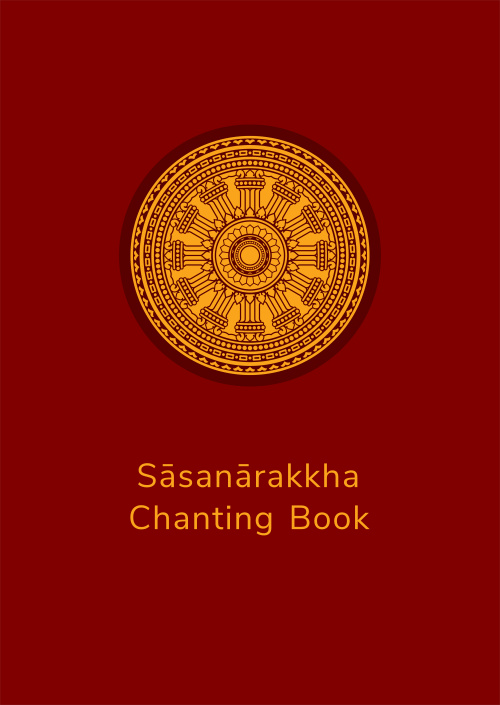
\includegraphics[height=\paperheight]{./reference-desktop-cover.jpg}}
\fi

\cleartorecto
\thispagestyle{empty}
\vspace*{5em}

{\centering

\settowidth{\titleLength}{%
  {\Large\chapterTitleFont\textls*{\MakeUppercase{\thetitle}}}%
}

{\Large\chapterTitleFont\textls*{\MakeUppercase{\thetitle}}}\\[0.3\baselineskip]
\setlength{\xheight}{\heightof{X}}
\raisebox{0.5\xheight}{\color[gray]{0.4}\rule{\titleLength}{0.25pt}}\\[0.3\baselineskip]
{\itshape \thesubtitle}

\vfill

\vspace*{5em}

}


\cleartoverso
\thispagestyle{empty}

\vspace*{-\baselineskip}

{%

\fontsize{9}{11}\selectfont
\centering
\setlength{\parindent}{0pt}%
\setlength{\parskip}{0.8\baselineskip}%

% \thetitle\\
% \thesubtitle

This book is offered for free distribution,\\
please do not sell this book.

Download this book in PDF, EPUB and MOBI formats\\
at the following address:

\href{https://sasanarakkha.org/}{sasanarakkha.org}

\vfill

Project Manager: Ā. Ariyadhammika\\
Editors: Ā. Devamitta, Ā. Pāladhammika, Ā. Pamodadhammika\\
Typesetting: Ā. Gambhiro, Ā. Pāladhammika\\
Translators: Ā. Aggacitta, Ā. Bodhi, Ā. Sujāto\\
Endnotes: Ā. Ariyadhammika

\vfill

This version was created on:\\
\today\\
\currenttime

\vfill

This work is licensed under a Creative Commons\\
Attribution-NonCommercial-NoDerivatives 4.0 International~License.

Produced with the \LaTeX\ typesetting system,\\
set in Libertinus Serif.

\theEditionInfo

}

\cleartorecto
\thispagestyle{empty}

{\setlength{\parskip}{10pt}

{\centering\fontsize{20}{25}\selectfont
\textsc{We Wish To Gratefully Acknowledge}
\par}

The Saṅghas of Wat Pah Nanachat (WPN), Amaravati, and Abhayagiri for allowing the use of material from their respective chanting books, the late Ven. Dr. Saddhātissa and Mr. Maurice Walshe for their English translations, as well as Ven. Bhikkhu Bodhi for granting permission to use and slightly adapt his translations. Further contributions are found on the previous page.

\vspace*{1.5\baselineskip}

Additional information on translations, as well as deviations\pagenote{%
  Due to the balanced and inspiring selction of chants, as well as for the sake of
  compatability, the WPN chanting book has served as the basis for the SBS
  chanting book. Over time, suggestions for the inclusion of additional chants, as
  well as occasional improvements of existing translations were incorporated. Such
  changes were meticulously marked down in the endnotes, so that someone familiar
  with the SBS chanting book can straight away find the relevant differences,
  which can be useful when visiting a branch monastery of the Ajahn Chah lineage,
  in order to know in which places to revert to the original version.}
from WPN Chanting Book (2014), have been annotated by Ven. Ariyadhammika in the endnotes.

\bigskip

{\centering
To Āyasmā Aggacitta, the founding father of\\
Sāsanārakkha Buddhist Sanctuary.

\bigskip


\includegraphics[height=65mm]{SBS_logo_Tuck_Loon_BAedit_2020_small.jpg}

}

}

% \chapter{Abbreviations}
\label{abbreviations}

\begin{tabular}{@{}ll@{}}
  \anglebracketleft\ \hspace{-0.5mm}... \hspace{-0.85mm}\anglebracketright\ & \hspace{7.35mm}Only recited by the leader \\
  \hspace{0.1cm} \abbrbreathmark\ & \hspace{7.35mm}Breathing pause \\
\end{tabular}

\begin{tabular}{@{}ll@{}}
  Vin   & Vinaya Piṭaka                                      \\
  DN    & Dīgha Nikāya                                       \\
  MN    & Majjhima Nikāya                                    \\
  SN    & Saṁyutta Nikāya                                    \\
  AN    & Aṅguttara Nikāya                                   \\
  Khp   & Khuddakapāṭha                                      \\
  Dhp   & Dhammapada                                         \\
  Ud    & Udāna                                              \\
  Snp   & Sutta Nipāta                                       \\
  Thag  & Theragāthā                                         \\
  Ja    & Jātaka                                             \\
  % Ps    & Paṭisambhidāmagga                                \\
  Vibh  & Abhidhamma Vibhaṅga                                \\
  Dhs   & Dhammasaṅganī                                      \\
  A     & Aṭṭhakathā (Commentary)                            \\
  MJG   & Mahā-jaya-maṅgala-gāthā (Sri Lanka)                \\
  Thai  & Composed in Thailand, normally in recent centuries \\
  Sri L & Composed in Sri Lanka                              \\
  Trad  & Traditional verses not found in the original Pāli  \\
  WPN  & Wat Pah Nanachat Buddhist Chanting (2014)           \\
\end{tabular}

\bigskip

Wisdom Publication sources: Nikāya and sutta \# (eg. DN 1)\\
P.T.S. sources: Nikāya, volume \#, page \# (eg. D i 1)


\cleartorecto
\pagestyle{toponerow-frontmatter}
\tableofcontents*

% \clearpage
% \listfirstlines*

\mainmatter
\pagestyle{toponerow}

\cleartorecto
\part{Pāli/English Recitations}

{\raggedright
HELLO
\chapter{Homage to the Triple Gem}

\section{Dedication of Offerings}

[Yo so] bhagavā arahaṁ sammāsambuddho

\begin{cprenglish}
  To the Blessed One the Worthy One who fully attained Perfect Enlightenment
\end{cprenglish}

Svākkhāto yena bhagavatā dhammo

\begin{cprenglish}
  To the Teaching which he expounded so well
\end{cprenglish}

Supaṭipanno yassa bhagavato sāvakasaṅgho

\begin{cprenglish}
  And to the Blessed One’s disciples who have practiced well
\end{cprenglish}

Tam-mayaṁ bhagavantaṁ sadhammaṁ sasaṅghaṁ

\begin{cprenglish}
  To these the Buddha the Dhamma and the Saṅgha
\end{cprenglish}

Imehi sakkārehi yathārahaṁ āropitehi abhipūjayāma

\begin{cprenglish}
  We render with offerings our rightful homage
\end{cprenglish}

Sādhu no bhante bhagavā sucira-parinibbutopi

\begin{cprenglish}
  It is well for us that the Blessed One\\
  Having attained liberation
\end{cprenglish}

Pacchimā-janatānukampa-mānasā

\begin{cprenglish}
  Still had compassion for later generations
\end{cprenglish}

Ime sakkāre duggata-paṇṇākāra-bhūte paṭiggaṇhātu

\begin{cprenglish}
  May these simple offerings be accepted
\end{cprenglish}

Amhākaṁ dīgharattaṁ hitāya sukhāya

\begin{cprenglish}
  For our long-lasting benefit and for the happiness it gives us
\end{cprenglish}

Arahaṁ sammāsambuddho bhagavā

\begin{cprenglish}
  The Worthy One the Perfectly Enlightened and Blessed One
\end{cprenglish}

Buddhaṁ bhagavantaṁ abhivādemi\relax

\begin{cprenglish}
  I render homage to the Buddha the Blessed One (Bow)
\end{cprenglish}

[Svākkhāto] bhagavatā dhammo

\begin{cprenglish}
  The Teaching so completely explained by him
\end{cprenglish}

Dhammaṁ namassāmi\relax

\begin{cprenglish}
  I bow to the Dhamma (Bow)
\end{cprenglish}

[Supaṭipanno] bhagavato sāvakasaṅgho

\begin{cprenglish}
  The Blessed One’s disciples who have practiced well
\end{cprenglish}

Saṅghaṁ namāmi

\begin{cprenglish}
  I bow to the Saṅgha (Bow)
\end{cprenglish}

\section{Preliminary Homage}

\begin{leader}
  [Handa mayaṁ buddhassa bhagavato pubbabhāga-namakāraṁ karomase]
\end{leader}
\begin{leader}
  [Now let us pay preliminary homage to the Buddha.]
\end{leader}

Namo tassa bhagavato arahato sammāsambuddhassa [3x]

\begin{cprenglish}
  Homage to the Blessed Worthy and Perfectly Enlightened One [3x]
\end{cprenglish}

\clearpage

\section{Homage to the Buddha}

\begin{leader}
  [Handa mayaṁ buddhābhitthutiṁ karomase]
\end{leader}
\begin{leader}
  [Now let us recite in praise of the Buddha]
\end{leader}

Yo so tathāgato arahaṁ sammāsambuddho

\begin{cprenglish}
  The Tathāgata is the Worthy One the Perfectly Enlightened One
\end{cprenglish}

Vijjācaraṇa-sampanno

\begin{cprenglish}
  He is impeccable in conduct and understanding
\end{cprenglish}

Sugato

\begin{cprenglish}
  The Accomplished One
\end{cprenglish}

Lokavidū

\begin{cprenglish}
  The Knower of the Worlds
\end{cprenglish}

Anuttaro purisadamma-sārathi

\begin{cprenglish}
  Unsurpassed leader of persons to be tamedi
\end{cprenglish}

Satthā deva-manussānaṁ

\begin{cprenglish}
  He is teacher of gods and humans
\end{cprenglish}

Buddho bhagavā

\begin{cprenglish}
  He is awake and holy
\end{cprenglish}

Yo imaṁ lokaṁ sadevakaṁ samārakaṁ sabrahmakaṁ

\begin{cprenglish}
  In this world with its gods ̓ demons and kind spirits
\end{cprenglish}

Sassamaṇa-brāhmaṇiṁ pajaṁ sadeva-manussaṁ sayaṁ abhiññā sacchikatvā pavedesi

\begin{cprenglish}
  Its seekers and sages  ̓  celestial and human beings\\
  He has by deep insight revealed the truth
\end{cprenglish}

Yo dhammaṁ desesi ādi-kalyāṇaṁ majjhe-kalyāṇaṁ pariyosāna-kalyāṇaṁ

\begin{cprenglish}
  He has pointed out the Dhamma\\
  Beautiful in the beginning\\
  Beautiful in the middle\\
  Beautiful in the end\\
\end{cprenglish}

Sātthaṁ sabyañjanaṁ kevala-paripuṇṇaṁ parisuddhaṁ brahma-cariyaṁ pakāsesi

\begin{cprenglish}
  He has explained the holy life of complete purity\\
  In its essence and conventions
\end{cprenglish}

Tam-ahaṁ bhagavantaṁ abhipūjayāmi tam-ahaṁ bhagavantaṁ sirasā namāmi
\begin{cprenglish}
  I chant my praise to the Blessed One\\
  I bow my head to the Blessed One (Bow)
\end{cprenglish}

\section{Homage to the Dhamma}

\begin{leader}
  [Handa mayaṁ dhammābhitthutiṁ karomase]
\end{leader}
\begin{leader}
  [Now let us recite in praise of the Dhamma]
\end{leader}

Yo so svākkhāto bhagavatā dhammo

\begin{cprenglish}
  The Dhamma is well-expounded by the Blessed One
\end{cprenglish}

Sandiṭṭhiko

\begin{cprenglish}
  Apparent here and now
\end{cprenglish}

Akāliko

\begin{cprenglish}
  Timeless
\end{cprenglish}

Ehipassiko

\begin{cprenglish}
  Encouraging investigation
\end{cprenglish}

Opanayiko

\begin{cprenglish}
  Leading inwards
\end{cprenglish}

Paccattaṁ veditabbo viññūhi

\begin{cprenglish}
  To be experienced individually by the wise
\end{cprenglish}

Tam-ahaṁ dhammaṁ abhipūjayāmi tam-ahaṁ dhammaṁ sirasā namāmi

\begin{cprenglish}
  I chant my praise to this teaching\\
  I bow my head to this truth (Bow)
\end{cprenglish}

\section{Homage to the Saṅgha}

\begin{leader}
  Handa mayaṁ saṅghābhitthutiṁ karomase
\end{leader}
\begin{leader}
  Now let us recite in praise of the Saṅgha
\end{leader}

Yo so supaṭipanno bhagavato sāvakasaṅgho

\begin{cprenglish}
  They are the Blessed One’s disciples who have practiced well
\end{cprenglish}

Ujupaṭipanno bhagavato sāvakasaṅgho

\begin{cprenglish}
  Who have practiced directly
\end{cprenglish}

Ñāyapaṭipanno bhagavato sāvakasaṅgho

\begin{cprenglish}
  Who have practiced correctlyi
\end{cprenglish}

Sāmīcipaṭipanno bhagavato sāvakasaṅgho

\begin{cprenglish}
  Who have practiced properlyi
\end{cprenglish}

Yadidaṁ cattāri purisayugāni aṭṭha purisapuggalā

\begin{cprenglish}
  That is the four pairs the eight kinds of Noble Beings
\end{cprenglish}

Esa bhagavato sāvakasaṅgho

\begin{cprenglish}
  These are the Blessed One’s disciples
\end{cprenglish}

Āhuneyyo

\begin{cprenglish}
  Such ones are worthy of gifts
\end{cprenglish}

Pāhuneyyo

\begin{cprenglish}
  Worthy of hospitality
\end{cprenglish}

Dakkhiṇeyyo

\begin{cprenglish}
  Worthy of offerings
\end{cprenglish}

Añjali-karaṇīyo

\begin{cprenglish}
  Worthy of respect
\end{cprenglish}

Anuttaraṁ puññakkhettaṁ lokassa

\begin{cprenglish}
  They give occasion for incomparable goodness to arise in the world
\end{cprenglish}

Tam-ahaṁ saṅghaṁ abhipūjayāmi tam-ahaṁ saṅghaṁ sirasā namāmi

\begin{cprenglish}
  I chant my praise to this Saṅgha\\
  I bow my head to this Saṅgha (Bow)
\end{cprenglish}


\section{Salutation to the Triple Gem}

\begin{leader}
  [Handa mayaṁ ratanattaya-paṇāma-gāthāyo c'eva saṁvega-parikittana-pāṭhañca bhaṇāmase]
\end{leader}
\begin{leader}
  [Now let us recite our salutation to the Triple Gem and a passage to arouse urgency]
\end{leader}

\firstline{Buddho susuddho karuṇā-mahaṇṇavo}

Buddho susuddho karuṇā-mahaṇṇavo

\begin{cprenglish}
  The Buddha absolutely pure with ocean-like compassion
\end{cprenglish}

Yo'ccanta-suddhabbara-ñāṇa-locano

\begin{cprenglish}
  Possessing the clear sight of wisdom
\end{cprenglish}

Lokassa pāpūpakilesa-ghātako

\begin{cprenglish}
  Destroyer of worldly self-corruption
\end{cprenglish}

Vandāmi buddhaṁ aham-ādarena taṁ

\begin{cprenglish}
  Devotedly indeed  ̓  that Buddha I revere
\end{cprenglish}

Dhammo padīpo viya tassa satthuno

\begin{cprenglish}
  The Teaching of the Lord is like a lamp
\end{cprenglish}

Yo magga-pākāmata-bheda-bhinnako

\begin{cprenglish}
  Divided into path and its fruit  ̓  the Deathless
\end{cprenglish}

Lokuttaro yo ca tad-attha-dīpano

\begin{cprenglish}
  And illuminating that goal  ̓  which is beyond the conditioned worldi
\end{cprenglish}

Vandāmi dhammaṁ aham-ādarena taṁ

\begin{cprenglish}
  Devotedly indeed  ̓  that Dhamma I revere
\end{cprenglish}

Saṅgho sukhettābhyati-khetta-saññito

\begin{cprenglish}
  The Saṅgha the most fertile ground for cultivation
\end{cprenglish}

Yo diṭṭha-santo sugatānubodhako

\begin{cprenglish}
  Those who have realised peace\\
  Awakened after the Accomplished One
\end{cprenglish}

Lolappahīno ariyo sumedhaso

\begin{cprenglish}
  Noble and wise  ̓  all longing abandoned
\end{cprenglish}

Vandāmi saṅghaṁ aham-ādarena taṁ

\begin{cprenglish}
  Devotedly indeed  ̓  that Saṅgha I revere
\end{cprenglish}

Iccevam-ekantabhipūja-neyyakaṁ vatthuttayaṁ vandayatābhisaṅkhataṁ

\begin{cprenglish}
  This salutation should be made\\
  To that triad which is worthy
\end{cprenglish}

Puññaṁ mayā yaṁ mama sabbupaddavā

\begin{cprenglish}
  Through the power of such good action
\end{cprenglish}

Mā hontu ve tassa pabhāva-siddhiyā

\begin{cprenglish}
  May all obstacles disappear
\end{cprenglish}

Idha tathāgato loke uppanno arahaṁ sammāsambuddho

\begin{cprenglish}
  One who knows things as they are  ̓  has arisen in this world\\
  And he is an Arahant  ̓  a perfectly awakened being
\end{cprenglish}

Dhammo ca desito niyyāniko upasamiko parinibbāniko sambodhagāmī sugatappavedito

\begin{cprenglish}
  Teaching the way leading out of delusion\\
  Calming and directing to perfect peace\\
  And leading to enlightenment\\
  This way he has made known\\
\end{cprenglish}

Mayan-taṁ dhammaṁ sutvā evaṁ jānāma

\begin{cprenglish}
  Having heard the Teaching we know this
\end{cprenglish}

Jātipi dukkhā

\begin{cprenglish}
  Birth is dukkha
\end{cprenglish}

Jarāpi dukkhā

\begin{cprenglish}
  Ageing is dukkha
\end{cprenglish}

Maraṇampi dukkhaṁ

\begin{cprenglish}
  And death is dukkha
\end{cprenglish}

Soka-parideva-dukkha-domanass'upāyāsāpi dukkhā

\begin{cprenglish}
  Sorrow lamentation pain displeasurei and despair are dukkha
\end{cprenglish}

Appiyehi sampayogo dukkho

\begin{cprenglish}
  Association with the disliked is dukkha
\end{cprenglish}

Piyehi vippayogo dukkho

\begin{cprenglish}
  Separation from the liked is dukkha
\end{cprenglish}

Yamp'icchaṁ na labhati tampi dukkhaṁ

\begin{cprenglish}
  Not attaining one’s wishes is dukkha
\end{cprenglish}

Saṅkhittena pañcupādānakkhandhā dukkhā

\begin{cprenglish}
  In brief  ̓  the five aggregates of clinging are dukkhai
\end{cprenglish}

Seyyathīdaṁ

\begin{cprenglish}
  These are as follows
\end{cprenglish}

Rūpūpādānakkhandho

\begin{cprenglish}
  Attachment to form
\end{cprenglish}

Vedanūpādānakkhandho

\begin{cprenglish}
  Attachment to feeling
\end{cprenglish}

Saññūpādānakkhandho

\begin{cprenglish}
  Attachment to perception
\end{cprenglish}

Saṅkhārūpādānakkhandho

\begin{cprenglish}
  Attachment to volitional formations
\end{cprenglish}

Viññāṇūpādānakkhandho

\begin{cprenglish}
  Attachment to consciousness
\end{cprenglish}

Yesaṁ pariññāya

\begin{cprenglish}
  For the complete understanding of this
\end{cprenglish}

Dharamāno so bhagavā

\begin{cprenglish}
  The Blessed One in his lifetime
\end{cprenglish}

Evaṁ bahulaṁ sāvake vineti

\begin{cprenglish}
  Frequently instructed his disciples in just this way
\end{cprenglish}

Evaṁ bhāgā ca panassa bhagavato sāvakesu anusāsanī bahulā pavattati

\begin{cprenglish}
  In addition he further instructed
\end{cprenglish}

Rūpaṁ aniccaṁ

\begin{cprenglish}
  Form is impermanent
\end{cprenglish}

Vedanā aniccā

\begin{cprenglish}
  Feeling is impermanent
\end{cprenglish}

Saññā aniccā

\begin{cprenglish}
  Perception is impermanent
\end{cprenglish}

Saṅkhārā aniccā

\begin{cprenglish}
  Volitional formations are impermanent
\end{cprenglish}

Viññāṇaṁ aniccaṁ

\begin{cprenglish}
  Consciousness is impermanent
\end{cprenglish}

Rūpaṁ anattā

\begin{cprenglish}
  Form is not-self
\end{cprenglish}

Vedanā anattā

\begin{cprenglish}
  Feeling is not-self
\end{cprenglish}

Saññā anattā

\begin{cprenglish}
  Perception is not-self
\end{cprenglish}

Saṅkhārā anattā

\begin{cprenglish}
  Volitional formations are not-self
\end{cprenglish}

Viññāṇaṁ anattā

\begin{cprenglish}
  Consciousness is not-self
\end{cprenglish}

Sabbe saṅkhārā aniccā

\begin{cprenglish}
  All conditioned things are impermanent
\end{cprenglish}

Sabbe dhammā anattā't

\begin{cprenglish}
  All things are not-self
\end{cprenglish}

Te mayaṁ otiṇṇāmha jātiyā jarā-maraṇena

\begin{cprenglish}
  All of us are affected by birth  ̓  ageing and deathi
\end{cprenglish}

Sokehi paridevehi dukkhehi domanassehi upāyāsehi

\begin{cprenglish}
  By sorrow lamentation pain displeasure and despair
\end{cprenglish}

Dukkhotiṇṇā dukkha-paretā

\begin{cprenglish}
  Affected by dukkha and afflicted by dukkha
\end{cprenglish}

Appeva nāmimassa kevalassa dukkha-kkhandhassa antakiriyā paññāyethā'ti

\begin{cprenglish}
  Let us all aspire to complete freedom from suffering
\end{cprenglish}

Cira-parinibbutampi taṁ bhagavantaṁ uddissa arahantaṁ sammāsambuddhaṁ

\begin{cprenglish}
  Remembering the Blessed One  ̓  the Worthy One  ̓  and Perfectly Enlightened One\\
  Who long ago attained Parinibbāna
\end{cprenglish}

Saddhā agārasmā anagāriyaṁ pabbajitā

\begin{cprenglish}
  We have gone forth with faith\\
  From home to homelessness
\end{cprenglish}

Tasmiṁ bhagavati brahma-cariyaṁ carāma

\begin{cprenglish}
  And like the Blessed One  ̓  we practice the holy life
\end{cprenglish}

Bhikkhūnaṁ sikkhāsājīva-samāpannā

\begin{cprenglish}
  Possessing the bhikkhus’ training and way of life
\end{cprenglish}

Taṁ no brahma-cariyaṁ imassa kevalassa dukkha-kkhandhassa antakiriyāya saṁvattatu

\begin{cprenglish}
  May this holy life  ̓  lead us to the end of this whole mass of suffering
\end{cprenglish}


\chapter{Verses}

\section{The Buddha's First Exclamation}
\paliTitle{Buddha-paṭhama-bhāsita}

\begin{twochants}
  Aneka-jāti-saṁsāraṁ & Sandhāvissaṁ anibbisaṁ\\
  Gaha-kāraṁ gavesanto & Dukkhā jāti punappunaṁ\\
\end{twochants}

\begin{english}
  For many lifetimes in the round of birth\\
  Wandering on endlessly\\
  For the builder of this house I searched\\
  How painful is repeated birth.
\end{english}

\begin{twochants}
  Gaha-kāraka diṭṭho'si & Puna gehaṁ na kāhasi\\
  Sabbā te phāsukā bhaggā & Gaha-kūṭaṁ visaṅkhataṁ\\
  Visaṅkhāra-gataṁ cittaṁ & Taṇhānaṁ khayam-ajjhagā\\
\end{twochants}

\begin{english}
  House-builder you've been seen\\
  Another home you will not build\\
  All your rafters have been snapped\\
  Dismantled is your ridge-pole\\
  The non-constructing mind\\
  Has come to craving's end
\end{english}

\suttaRef{Dhp 153-154}

\clearpage

\section{Respect for the Dhamma}
\paliTitle{Dhamma-gārava}

\begin{twochants}
  Ye ca atītā sambuddhā & Ye ca buddhā anāgatā \\
  Yo c'etarahi sambuddho & Bahunnaṃ soka-nāsano \\
\end{twochants}

\begin{english}
  All the Buddhas of the past\\
  All the Buddhas yet to come\\
  The Buddha of this current age\\
  Dispellers of much sorrow
\end{english}

\begin{twochants}
  Sabbe saddhamma-garuno & Vihariṃsu viharanti ca\\
  Atho pi viharissanti & Esā buddhāna dhammatā\\
\end{twochants}

\begin{english}
  Those having lived or living now\\
  Those living in the future\\
  All do revere the True Dhamma\\
  That is the nature of all Buddhas
\end{english}

\begin{twochants}
  Tasmā hi atta-kāmena & Mahattam-abhikaṅkhatā\\
  Saddhammo garu-kātabbo & Saraṃ buddhāna sāsanaṃ\\
\end{twochants}

\begin{english}
  Therefore desiring one's own welfare\\
  Pursuing greatest aspirations\\
  One should revere the True Dhamma\\
  Recollecting the Buddha's teaching
\end{english}

\suttaRef{SN 6.2}

\begin{paritta}
  Na hi dhammo adhammo ca\\
  Ubho sama-vipākino\\
  Adhammo nirayaṃ neti\\
  Dhammo pāpeti suggatiṃ
\end{paritta}

\begin{english}
  What is true Dhamma and what's not\\
  Will never have the same results\\
  While wrong Dhamma leads to hell realms\\
  True Dhamma takes one on a good course
\end{english}

\begin{paritta}
  Dhammo have rakkhati dhamma-cāriṃ\\
  Dhammo suciṇṇo sukham-āvahāti\\
  Esānisaṃso dhamme suciṇṇe\\
  Na duggatiṃ gacchati dhamma-cārī
\end{paritta}

\clearpage

\begin{english}
  The Dhamma guards those who live in line with it\\
  And leads to happiness when practised well\\
  This is the blessing of well-practised Dhamma\\
  The Dhamma-farer does not go on a bad course
\end{english}

\suttaRef{Thag 4.10}

\clearpage

\section{Going to True and False Refuges}
\paliTitle{Khemākhema-saraṇa-gamana}

\begin{twochants}
  Bahuṃ ve saraṇaṃ yanti & Pabbatāni vanāni ca\\
  Ārāma-rukkha-cetyāni & Manussā bhaya-tajjitā\\
\end{twochants}

\begin{english}
  To many refuges they go\\
  To mountain slopes and forest glades\\
  To parkland shrines and sacred sites\\
  People overcome by fear
\end{english}

\begin{twochants}
  N'etaṃ kho saraṇaṃ khemaṃ & N'etaṃ saraṇam-uttamaṃ\\
  N'etaṃ saraṇam-āgamma & Sabba-dukkhā pamuccati\\
\end{twochants}

\begin{english}
  Such a refuge is not secure\\
  Such a refuge is not supreme\\
  Such a refuge does not bring\\
  Complete release from all suffering
\end{english}

\begin{twochants}
  Yo ca buddhañ-ca dhammañ-ca & Saṅghañ-ca saraṇaṃ gato\\
  Cattāri ariya-saccāni & Sammappaññāya passati\\
\end{twochants}

\begin{english}
  Whoever goes to refuge\\
  In the Triple Gem\\
  Sees with right discernment\\
  The Four Noble Truths
\end{english}

\begin{twochants}
  Dukkhaṃ dukkha-samuppādaṃ & Dukkhassa ca atikkamaṃ\\
  Ariyañ-c'aṭṭh'aṅgikaṃ maggaṃ & Dukkhūpasama-gāminaṃ\\
\end{twochants}

\begin{english}
  Suffering and its origin\\
  And that which lies beyond\\
  The Noble Eightfold Path\\
  That leads the way to suffering's end.
\end{english}

\begin{twochants}
  Etaṃ kho saraṇaṃ khemaṃ & Etaṃ saraṇam-uttamaṃ\\
  Etaṃ saraṇam-āgamma & Sabba-dukkhā pamuccatī'ti.
\end{twochants}

\begin{english}
  Such a refuge is secure\\
  Such a refuge is supreme\\
  Such a refuge truly brings\\
  Complete release from all suffering.
\end{english}

\suttaRef{Dhp 188-192}

\section{The Pāṭimokkha Exhortation}
\paliTitle{Ovāda-pāṭimokkha-gāthā}

\begin{leader}
  [Handa mayaṃ ovāda-pāṭimokkha-gāthāyo bhaṇāmase]
\end{leader}

Sabba-pāpassa akaraṇaṃ

\begin{cprenglish}
  Not doing any evil
\end{cprenglish}

Kusalassūpasampadā

\begin{cprenglish}
  To be committed to the good
\end{cprenglish}

Sacitta-pariyodapanaṃ

\begin{cprenglish}
  To purify one's mind
\end{cprenglish}

Etaṃ buddhāna sāsanaṃ

\begin{cprenglish}
  These are the teachings of all Buddhas
\end{cprenglish}

Khantī paramaṃ tapo tītikkhā

\begin{cprenglish}
  Patient endurance is the highest practice burning out defilements
\end{cprenglish}

Nibbānaṃ paramaṃ vadanti buddhā

\begin{cprenglish}
  The Buddhas say Nibbāna is supreme
\end{cprenglish}

Na hi pabbajito parūpaghātī

\begin{cprenglish}
  Not a renunciant is one who injures others
\end{cprenglish}

Samaṇo hoti paraṃ viheṭhayanto

\begin{cprenglish}
  Whoever troubles others can't be called a monk
\end{cprenglish}

Anūpavādo anūpaghāto

\begin{cprenglish}
  Not to insult and not to injure
\end{cprenglish}

Pāṭimokkhe ca saṃvaro

\begin{cprenglish}
  To live restrained by training rules
\end{cprenglish}

Mattaññutā ca bhattasmiṃ

\begin{cprenglish}
  Knowing one's measure at the meal
\end{cprenglish}

Pantañca sayan'āsanaṃ

\begin{cprenglish}
  Retreating to a lonely place
\end{cprenglish}

Adhicitte ca āyogo

\begin{cprenglish}
  Devotion to the higher mind
\end{cprenglish}

Etaṃ buddhāna sāsanaṃ

\begin{cprenglish}
  These are the teachings of all Buddhas
\end{cprenglish}

\suttaRef{Dhp 183-185}

\section{The Three Characteristics}
\paliTitle{Ti-lakkhaṇā}

\begin{leader}
  [Handa mayaṁ ti-lakkhaṇ’ādi-gāthāyo bhaṇāmase]
\end{leader}

\begin{twochants}
  Sabbe saṅkhārā aniccā’ti & Yadā paññāya passati\\
  Atha nibbindati dukkhe & Esa maggo visuddhiyā\\
\end{twochants}

\begin{english}
  “All conditioned things are impermanent”\\
  When with wisdom this is seen\\
  One feels weary of all dukkha\\
  This is the path to purity
\end{english}

\begin{twochants}
  Sabbe saṅkhārā dukkhā’ti & Yadā paññāya passati\\
  Atha nibbindati dukkhe & Esa maggo visuddhiyā\\
\end{twochants}

\begin{english}
  “All conditioned things are dukkha”\\
  When with wisdom this is seen\\
  One feels weary of all dukkha\\
  This is the path to purity
\end{english}

\begin{twochants}
  Sabbe dhammā anattā’ti & Yadā paññāya passati\\
  Atha nibbindati dukkhe & Esa maggo visuddhiyā\\
\end{twochants}

\begin{english}
  “All things are not-self”\\
  When with wisdom this is seen\\
  One feels weary of all dukkha\\
  This is the path to purity
\end{english}

\suttaRef{Dhp 183-185}

\begin{twochants}
  Appakā te manussesu & Ye janā pāra-gāmino\\
  Athāyaṁ itarā pajā & Tīram-evānudhāvati\\
\end{twochants}

\begin{english}
  Few amongst humankind\\
  Are those who go beyond\\
  Yet there are the many folks\\
  Ever wandering on this shore
\end{english}

\begin{twochants}
  Ye ca kho sammad-akkhāte & Dhamme dhammānuvattino\\
  Te janā pāram-essanti & Maccu-dheyyaṁ suduttaraṁ\\
\end{twochants}

\begin{english}
  Wherever Dhamma is well-taught\\
  Those who train in line with it\\
  Are the ones who will cross over\\
  The realm of death so hard to flee
\end{english}

\begin{twochants}
  Kaṇhaṁ dhammaṁ vippahāya & Sukkaṁ bhāvetha paṇḍito\\
  Okā anokam-āgamma & Viveke yattha dūramaṁ\\
  Tatrābhiratim-iccheyya & Hitvā kāme akiñcano
\end{twochants}

\begin{english}
  Abandoning the darker states\\
  The wise pursue the bright\\
  Gone from home to homelessness\\
  Living withdrawn so hard to enjoy\\
  Such rare delight one should desire\\
  Sense pleasures cast away\\
  Not having anything
\end{english}

\suttaRef{Dhp 85-87.5}

\clearpage

\section{The Burdens}
\paliTitle{Bhārā}

\begin{leader}
[Handa mayaṁ bhāra-sutta-gāthāyo bhaṇāmase]
\end{leader}

\begin{twochants}
  Bhārā have pañcakkhandhā & Bhāra-hāro ca puggalo \\
  Bhār'ādānaṃ dukkhaṃ loke & Bhāra-nikkhepanaṃ sukhaṃ \\
\end{twochants}

\begin{english}
  The five aggregates indeed are burdens\\
  The beast of burden is the person\\
  In this world to take up burdens is dukkha\\
  Putting them down brings happiness
\end{english}

\begin{twochants}
  Nikkhipitvā garuṃ bhāraṃ & Aññaṃ bhāraṃ anādiya\\
  Samūlaṃ taṇhaṃ abbuyha & Nicchāto parinibbuto\\
\end{twochants}

\begin{english}
  A heavy burden cast away\\
  Not taking on another load\\
  With craving pulled out from the root\\
  Desires stilled, one is released
\end{english}

\suttaRef{SN 22.22}

\clearpage

\section{From the Elder Raṭṭhapāla}
\paliTitle{Raṭṭhapāla-thera-gāthā}

\begin{leader}
[Handa mayaṁ raṭṭhapālatthera-gāthāyo bhaṇāmase]
\end{leader}

\begin{twochants}
Passa cittakataṁ bimbaṁ –Arukāyaṁ samussitaṁ
Āturaṁ bahusaṅkappaṁ – Yassa natthi dhuvaṁ ṭhiti
\end{twochants}

\begin{english}
See this fancy puppet
A body built of sores
Diseased  ̓  obsessed over
Which does not last at all
\end{english}

\begin{twochants}
Passa cittakataṁ rūpaṁ – Maṇinā kuṇḍalena ca
Aṭṭhiṁ tacena onaddhaṁ – Saha vatthehi sobhati
\end{twochants}

\begin{english}
See this fancy figure
With its gems and earrings
It is bones wrapped in skin
Made pretty by its clothes
\end{english}

\begin{twochants}
Alattakakatā pādā – Mukhaṁ cuṇṇakamakkhitaṁ
Alaṁ bālassa mohāya – No ca pāragavesino
\end{twochants}

\begin{english}
Feet adorned with henna dye
And powder smeared upon its face
May be enough to beguile a fool
But not a seeker of the far shore
\end{english}

\begin{twochants}
Aṭṭhapadakatā kesā – Nettā añjanamakkhitā
Alaṁ bālassa mohāya – No ca pāragavesino
\end{twochants}

\begin{english}
Hair in eight braids
And eyeliner
May be enough to beguile a fool
But not a seeker of the far shore
\end{english}

\begin{twochants}
Añjanīva navā cittā – Pūtikāyo alaṅkato
Alaṁ bālassa mohāya – No ca pāragavesino
\end{twochants}

\begin{english}
A rotting body all adorned
Like a freshly painted unguent pot
May be enough to beguile a fool
But not a seeker of the far shore
\end{english}

\begin{twochants}
Passāmi loke sadhane manusse
Laddhāna vittaṁ na dadanti mohā
Luddhā dhanaṁ sannicayaṁ karonti
Bhiyyova kāme abhipatthayanti
\end{twochants}

\begin{english}
I see rich people in the world
Who from delusion give not the wealth they’ve earned
Greedily they hoard their riches
Yearning for ever more sense pleasures
\end{english}

\begin{twochants}
Rājā ca aññe ca bahū manussā
Avītataṇhā maraṇaṁ upenti
Ūnāva hutvāna jahanti dehaṁ
Kāmehi lokamhi na hatthi titti
\end{twochants}

\begin{english}
Not just the king but others too
Reach death not rid of craving
They leave the body still wanting
For in this world sense pleasures never satisfy
\end{english}

\begin{twochants}
Na dīghamāyuṁ labhate dhanena
Na cāpi vittena jaraṁ vihanti
Appaṁ hidaṁ jīvitamāhu dhīrā
Asassataṁ vippariṇāma-dhammaṁ
\end{twochants}

\begin{english}
Longevity is not gained by riches
Nor does wealth banish ageing
For the wise say this life is short
Subject to change  ̓  and not eternal
\end{english}

\begin{twochants}
Tasmā hi paññāva dhanena seyyā
Yāya vosānamidhādhigacchati
Abyositattā hi bhavābhavesu
Pāpāni kammāni karoti mohā
\end{twochants}

\begin{english}
Therefore wisdom is much better than wealth
By which one reaches perfection in this life
People through ignorance do evil deeds
Failing to reach the goal  ̓  from life to life
\end{english}

\begin{twochants}
Kāmā hi citrā madhurā manoramā
Virūparūpena mathenti cittaṁ
Ādīnavaṁ kāmaguṇesu disvā
Tasmā ahaṁ pabbajitomhi rāja
\end{twochants}

\begin{english}
Sense pleasures are diverse  ̓  sweet  ̓  delightful
Appearing in disguise they disturb the mind
Seeing danger in the cords of sense pleasure
Therefore I went forth O King
\end{english}

\begin{twochants}
Dumapphalānīva patanti māṇavā
Daharā ca vuḍḍhā ca sarīrabhedā
Etampi disvā pabbajitomhi rāja
Apaṇṇakaṁ sāmaññameva seyyo
\end{twochants}

\begin{english}
As fruits fall from a tree  ̓  so people fall
Young and old  ̓  when the body breaks up
Seeing this too I went forth O King
Surely the ascetic life is better
\end{english}

\suttaRef{Thag 16.4 / MN 82}

\clearpage

\section{From the Elder Pārāpariya}
\paliTitle{Pārāpariya-thera-gāthā}

\begin{leader}
[Handa mayaṁ pārāpariyatthera-gāthāyo bhaṇāmase]
\end{leader}

\begin{twochants}
Aññathā lokanāthamhi – Tiṭṭhante purisuttame
Iriyaṁ āsi bhikkhūnaṁ – Aññathā dāni dissati
\end{twochants}

\begin{english}
The behavior of the bhikkhus
These days seems different
From when the protector of the world
The best of men was still here
\end{english}

\begin{twochants}
Sītavātaparittāṇaṁ – Hirikopīnachādanaṁ
Mattaṭṭhiyaṁ abhuñjiṁsu – Santuṭṭhā itarītare
\end{twochants}

\begin{english}
Their robes were just for modesty
And protection from cold and wind
They ate in moderation
Content with whatever they were offered
\end{english}

\begin{twochants}
Paṇītaṁ yadi vā lūkhaṁ – Appaṁ vā yadi vā bahuṁ
Yāpanatthaṁ abhuñjiṁsu – Agiddhā nādhimucchitā
\end{twochants}

\begin{english}
Whether food was refined or rough
A little or a lot
They ate only for sustenance
Without greed or gluttony
\end{english}

\begin{twochants}
Jīvitānaṁ parikkhāre – Bhesajje atha paccaye
Na bāḷhaṁ ussukā āsuṁ – Yathā te āsavakkhaye
\end{twochants}

\begin{english}
They were not so eager
For the requisites of life
Such as tonics and other supplies
As they were for destructing the defilements
\end{english}

\begin{twochants}
Araññe rukkhamūlesu – Kandarāsu guhāsu ca
Vivekamanubrūhantā – Vihaṁsu tapparāyaṇā
\end{twochants}

\begin{english}
In the wilderness  ̓  at the foot of a tree
In caves and caverns
Fostering seclusion
They lived with that as their final goal
\end{english}

\begin{twochants}
Nīcā niviṭṭhā subharā – Mudū atthaddhamānasā
Abyāsekā amukharā – Atthacintā vasānugā
\end{twochants}

\begin{english}
They were used to simple things  ̓  easy to look after
Gentle  ̓  not stubborn at heart
Unsullied  ̓  not gossipy
Their thoughts were intent on the goal
\end{english}

\begin{twochants}
Tato pāsādikaṁ āsi – Gataṁ bhuttaṁ nisevitaṁ
Siniddhā teladhārāva – Ahosi iriyāpatho
\end{twochants}

\begin{english}
That’s why they inspired confidence
In their movements eating and practice
Their deportment was as smooth
As a stream of oil
\end{english}

\begin{twochants}
Yathā kaṇṭakaṭṭhānamhi – Careyya anupāhano
Satiṁ upaṭṭhapetvāna – Evaṁ gāme munī care
\end{twochants}

\begin{english}
When barefoot on a thorny path
One would walk
Quite mindfully
That’s how a sage should walk in the village
\end{english}

\begin{twochants}
Saritvā pubbake yogī – Tesaṁ vattamanussaraṁ
Kiñcāpi pacchimo kālo – Phuseyya amataṁ padaṁ
\end{twochants}

\begin{english}
Remembering the meditators of old
And recollecting their conduct
Even in the latter days
The Deathless can still be reached
\end{english}

\suttaRef{Thag 16.10}

\clearpage

\section{On Protection}
\paliTitle{Tāyana-gāthā}

\begin{leader}
[Handa mayaṁ Tāyana-gāthāyo bhaṇāmase]
\end{leader}

\begin{twochants}
Chinda sotaṁ parakkamma – Kāme panūda brāhmaṇa
Nappahāya muni kāme – Nekattam-upapajjati
\end{twochants}

\begin{english}
Exert yourself and cut the stream
Discard sense pleasures holy man
Not letting sensual pleasures go
A sage will not reach unityi
\end{english}

\begin{twochants}
Kayirā ce kayirāthenaṁ – Daḷham-enaṁ parakkame
Sithilo hi paribbājo – Bhiyyo ākirate rajaṁ
\end{twochants}

\begin{english}
Vigorously with all one’s strength
It should be done what should be done
A lax monastic life stirs up
The dust of defilements all the more
\end{english}

\begin{twochants}
Akataṁ dukkaṭaṁ seyyo – Pacchā tappati dukkaṭaṁ
Katañ-ca sukataṁ seyyo – Yaṁ katvā nānutappati
\end{twochants}

\begin{english}
Better is not to do bad deeds
That afterwards would bring remorse
It’s rather good deeds one should do
Which having done one won’t regret
\end{english}

\begin{twochants}
Kuso yathā duggahito – Hattham-evānukantati
Sāmaññaṁ dupparāmaṭṭhaṁ – Nirayāy’ūpakaḍḍhati
\end{twochants}

\begin{english}
As kusa grass when wrongly grasped
Will only cut into one’s hand
So does the monk’s life wrongly led
Indeed drag one to hellish states
\end{english}

\begin{twochants}
Yaṁ-kiñci sithilaṁ kammaṁ – Saṅkiliṭṭhañ-ca yaṁ vataṁ
Saṅkassaraṁ brahma-cariyaṁ – Na taṁ hoti mahapphalan’ti
\end{twochants}

\begin{english}
Whatever deed that’s slackly done
Whatever vow corruptly kept
The holy life led in doubtful ways
All these will never bear great fruits
\end{english}

\suttaRef{SN 2.8}

\clearpage

\section{Misecellaneous Verses}
\paliTitle{Pakiṇṇaka-gāthā}

\begin{leader}
[Handa mayaṁ pakiṇṇaka-gāthāyo bhaṇāmase]
\end{leader}

\begin{twochants}
Attadīpā bhikkhave viharatha attasaraṇā anaññasaraṇā
Dhammadīpā dhammasaraṇā anaññasaraṇā
\end{twochants}

\begin{english}
Bhikkhus dwell with yourselves as an island
With yourselves as a refuge  ̓  with no other refuge
With the Dhamma as an island  ̓  with the Dhamma as a refuge
With no other refuge
\end{english}

\suttaRef{SN 22.43}

\begin{twochants}
Appassutāyaṁ puriso – Balibaddova jīrati
Maṁsāni tassa vaḍḍhanti – Paññā tassa na vaḍḍhati
\end{twochants}

\begin{english}
The man of little learning
Grows old like an ox
He grows only in bulk
But his wisdom does not grow
\end{english}

\suttaRef{Dhp 152}

\begin{twochants}
Uyyuñjanti satīmanto – Na nikete ramanti te
Haṁsāva pallalaṁ hitvā – Okamokaṁ jahanti te
\end{twochants}

\begin{english}
The mindful ones exert themselves
They are not attached to any home
Like swans that abandon the lake
They leave home after home behind
\end{english}

\suttaRef{Dhp 91}

\begin{twochants}
Yaṁ pubbe taṁ visosehi – Pacchā te māhu kiñcanaṁ
Majjhe ce no gahessasi – Upasanto carissasi
\end{twochants}

\begin{english}
Dry up what pertains to the past
Let there be nothing afterward
If you do not grasp in the middle
You will live at peace
\end{english}

\suttaRef{Snp 949}

\begin{twochants}
Uṭṭhahatha nisīdatha – Ko attho supitena vo
Āturānañhi kā niddā – Sallaviddhāna ruppataṁ
\end{twochants}

\begin{english}
Arouse yourselves  ̓  sit up!
What good to you is sleeping?
For what sleep can there be for the afflicted
For those injured  ̓  pierced by the dart?
\end{english}

\begin{twochants}
Uṭṭhahatha nisīdatha – Daḷhaṁ sikkhatha santiyā
Mā vo pamatte viññāya – Maccurājā amohayittha vasānuge
\end{twochants}

\begin{english}
Arouse yourselves  ̓  sit up!
Train vigorously for the state of peace
Let not the King of Death catch you heedless
And delude you when under his control
\end{english}

\begin{twochants}
Yāya devā manussā ca – Sitā tiṭṭhanti atthikā
Tarathetaṁ visattikaṁ – Khaṇo vo mā upaccagā
Khaṇātītā hi socanti – Nirayamhi samappitā
\end{twochants}

\begin{english}
Cross over this attachment
By which devas and human beings
Full of need are held fast
Don’t let the opportunity pass you by
For those who have missed the opportunity
Sorrow when they arrive in hell
\end{english}

\begin{twochants}
Pamādo rajo pamādo – Pamādānupatito rajo
Appamādena vijjāya – Abbahe sallamattanoti
\end{twochants}

\begin{english}
Heedlessness is dust always
Dust follows upon heedlessness
By heedfulness by clear knowledge
Draw out the dart from yourself
\end{english}

\suttaRef{Snp 333-336}

\begin{twochants}
Piyato jāyatī soko – Piyato jāyatī bhayaṁ
Piyato vippamuttassa – Natthi soko kuto bhayaṁ
\end{twochants}

\begin{english}
From endearment springs sorrow
From endearment springs fear
For one who is free from endearment
There is no sorrow  ̓  whence then fear?
\end{english}

\suttaRef{Dhp 212}

\begin{twochants}
Tiṭṭhateva nibbānaṁ
\end{twochants}

\begin{english}
Nibbāna exists
\end{english}

\begin{twochants}
Tiṭṭhati nibbānagāmī maggo
\end{twochants}

\begin{english}
The path leading to nibbāna exists
\end{english}

\begin{twochants}
Maggakkhāyī tathāgato
\end{twochants}

\begin{english}
A Tathāgata is one who shows the path
\end{english}

\suttaRef{MN 107}

\begin{twochants}
Tumhehi kiccam-ātappaṃ
\end{twochants}

\begin{english}
You yourselves must strive
\end{english}

\suttaRef{Dhp 276}

\begin{twochants}
Yaṁ bhikkhave satthārā karaṇīyaṁ sāvakānaṁ
Hitesinā anukampakena anukampaṁ upādāya
\end{twochants}

\begin{english}
Bhikkhus what should be done for his disciples\\
Out of compassion by a teacher\\
Who seek their welfare and has compassion for them
\end{english}

\begin{twochants}
Kataṁ vo taṁ mayā
\end{twochants}

\begin{english}
That I have done for you
\end{english}

\begin{twochants}
Etāni bhikkhave rukkhamūlāni
\end{twochants}

\begin{english}
Bhikkhus these are roots of trees
\end{english}

\begin{twochants}
Etāni suññāgārāni
\end{twochants}

\begin{english}
These are empty huts
\end{english}

\begin{twochants}
Jhāyatha bhikkhave mā pamādattha
\end{twochants}

\begin{english}
Meditate bhikkhus  ̓  do not be negligent
\end{english}

\begin{twochants}
Mā pacchā vippaṭisārino ahuvattha
\end{twochants}

\begin{english}
Lest you regret it later
\end{english}

\begin{twochants}
Ayaṁ vo amhākaṁ anusāsanī’ti
\end{twochants}

\begin{english}
This is my instruction to you
\end{english}

\suttaRef{MN 19}

\chapter{Teachings}

\section*{Setting in Motion the Wheel of Dhamma}
\paliTitle{Dhamma-cakkappavattana}

\begin{leader}
[Handa mayaṁ dhamma-cakkappavattana sutta-pāṭhaṁ bhaṇāmase]
\end{leader}

Dveme bhikkhave antā

\begin{cprenglish}
Bhikkhus there are these two extremes
\end{cprenglish}

Pabbajitena na sevitabbā

\begin{cprenglish}
That should not be pursued  ̓  by one who has gone forth
\end{cprenglish}

Yo cāyaṁ kāmesu kāma-sukh’allikānuyogo

\begin{cprenglish}
That is whatever is tied up to sense pleasures\\
Within the realm of sensuality
\end{cprenglish}

Hīno

\begin{cprenglish}
Which is low
\end{cprenglish}

Gammo

\begin{cprenglish}
Common
\end{cprenglish}

Pothujjaniko

\begin{cprenglish}
The way of the common folk
\end{cprenglish}

Anariyo

\begin{cprenglish}
Not the way of the Noble Ones
\end{cprenglish}

Anattha-sañhito

\begin{cprenglish}
And pointless
\end{cprenglish}

Yo cāyaṁ atta-kilamathānuyogo

\begin{cprenglish}
Then there is whatever is tied up\\
With self-deprivation
\end{cprenglish}

Dukkho

\begin{cprenglish}
Which is painful
\end{cprenglish}

Anariyo

\begin{cprenglish}
Not the way of the Noble Ones
\end{cprenglish}

Anattha-sañhito

\begin{cprenglish}
And pointless
\end{cprenglish}

Ete te bhikkhave ubho ante anupagamma majjhimā paṭipadā tathāgatena abhisambuddhā

\begin{cprenglish}
Bhikkhus without going to either of these extremes\\
The Tathāgata has ultimately awakened\\
To a middle way of practice
\end{cprenglish}

Cakkhu-karaṇī

\begin{cprenglish}
Giving rise to vision
\end{cprenglish}

Ñāṇa-karaṇī

\begin{cprenglish}
Making for insight
\end{cprenglish}

Upasamāya

\begin{cprenglish}
Leading to calm
\end{cprenglish}

Abhiññāya

\begin{cprenglish}
To heightened knowing
\end{cprenglish}

Sambodhāya

\begin{cprenglish}
Awakening
\end{cprenglish}

Nibbānāya saṁvattati

\begin{cprenglish}
And to Nibbāna
\end{cprenglish}

Katamā ca sā bhikkhave majjhimā paṭipadā

\begin{cprenglish}
And what bhikkhus is that middle way of practice?
\end{cprenglish}

Ayam-eva ariyo aṭṭhaṅgiko maggo

\begin{cprenglish}
It is just this Noble Eightfold Path
\end{cprenglish}

Seyyathīdaṁ

\begin{cprenglish}
Which is as follows
\end{cprenglish}

Sammā-diṭṭhi

\begin{cprenglish}
Right View
\end{cprenglish}

Sammā-saṅkappo

\begin{cprenglish}
Right Intention
\end{cprenglish}

Sammā-vācā

\begin{cprenglish}
Right Speech
\end{cprenglish}

Sammā-kammanto

\begin{cprenglish}
Right Action
\end{cprenglish}

Sammā-ājīvo

\begin{cprenglish}
Right Livelihood
\end{cprenglish}

Sammā-vāyāmo

\begin{cprenglish}
Right Effort
\end{cprenglish}

Sammā-sati

\begin{cprenglish}
Right Mindfulness
\end{cprenglish}

Sammā-samādhi

\begin{cprenglish}
Right Concentration
\end{cprenglish}

Ayaṁ kho sā bhikkhave majjhimā paṭipadā tathāgatena abhisambuddhā

\begin{cprenglish}
This bhikkhus is the middle way of practice\\
That the Tathāgata has ultimately awakened to
\end{cprenglish}

Cakkhu-karaṇī

\begin{cprenglish}
Giving rise to vision
\end{cprenglish}

Ñāṇa-karaṇī

\begin{cprenglish}
Making for insight
\end{cprenglish}

Upasamāya

\begin{cprenglish}
Leading to calm
\end{cprenglish}

Abhiññāya

\begin{cprenglish}
To heightened knowing
\end{cprenglish}

Sambodhāya

\begin{cprenglish}
Awakening
\end{cprenglish}

Nibbānāya saṁvattati

\begin{cprenglish}
And to Nibbāna
\end{cprenglish}

Idaṁ kho pana bhikkhave dukkhaṁ ariya-saccaṁ

\begin{cprenglish}
This bhikkhus is the Noble Truth of dukkha
\end{cprenglish}

Jātipi dukkhā

\begin{cprenglish}
Birth is dukkha
\end{cprenglish}

Jarāpi dukkhā

\begin{cprenglish}
Ageing is dukkha
\end{cprenglish}

Byādhipi dukkho

\begin{cprenglish}
Sickness is dukkha
\end{cprenglish}

Maraṇampi dukkhaṁ

\begin{cprenglish}
And death is dukkha
\end{cprenglish}

Soka-parideva-dukkha-domanassupāyāsāpi dukkhā

\begin{cprenglish}
Sorrow lamentation pain displeasure and despair are dukkha
\end{cprenglish}

Appiyehi sampayogo dukkho

\begin{cprenglish}
Association with the disliked is dukkha
\end{cprenglish}

Piyehi vippayogo dukkho

\begin{cprenglish}
Separation from the liked is dukkha
\end{cprenglish}

Yampicchaṁ na labhati tampi dukkhaṁ

\begin{cprenglish}
Not attaining one’s wishes is dukkha
\end{cprenglish}

Saṅkhittena pañcupādānakkhandhā dukkhā

\begin{cprenglish}
In brief  ̓  the five aggregates of clinging are dukkha
\end{cprenglish}

Idaṁ kho pana bhikkhave dukkha-samudayo ariya-saccaṁ

\begin{cprenglish}
This bhikkhus is the Noble Truth of the origin of dukkha
\end{cprenglish}

Yā’yaṁ taṇhā

\begin{cprenglish}
It is this craving
\end{cprenglish}

Ponobbhavikā

\begin{cprenglish}
Which leads to rebirth
\end{cprenglish}

Nandi-rāga-sahagatā

\begin{cprenglish}
Accompanied by delight and lust
\end{cprenglish}

Tatra-tatrābhinandinī

\begin{cprenglish}
Delighting now here now there
\end{cprenglish}

Seyyathīdaṁ

\begin{cprenglish}
Which is as follows
\end{cprenglish}

Kāma-taṇhā

\begin{cprenglish}
Craving for sensuality
\end{cprenglish}

Bhava-taṇhā

\begin{cprenglish}
Craving to become
\end{cprenglish}

Vibhava-taṇhā

\begin{cprenglish}
Craving not to become
\end{cprenglish}

Idaṁ kho pana bhikkhave dukkha-nirodho ariya-saccaṁ

\begin{cprenglish}
This bhikkhus is the Noble Truth of the cessation of dukkha
\end{cprenglish}

Yo tassāy’eva taṇhāya asesa-virāga-nirodho

\begin{cprenglish}
It is the remainderless fading away and cessation\\
Of that very craving
\end{cprenglish}

Cāgo

\begin{cprenglish}
Its relinquishment
\end{cprenglish}

Paṭinissaggo

\begin{cprenglish}
Letting go
\end{cprenglish}

Mutti

\begin{cprenglish}
Release
\end{cprenglish}

Anālayo

\begin{cprenglish}
Without any attachment
\end{cprenglish}

Idaṁ kho pana bhikkhave dukkha-nirodha-gāminī-paṭipadā ariya-saccaṁ

\begin{cprenglish}
This bhikkhus is the Noble Truth of the way of practice\\
Leading to the cessation of dukkha
\end{cprenglish}

Ayam-eva ariyo aṭṭh’aṅgiko maggo

\begin{cprenglish}
It is just this Noble Eightfold Path
\end{cprenglish}

Seyyathīdaṁ

\begin{cprenglish}
Which is as follows
\end{cprenglish}

Sammā-diṭṭhi

\begin{cprenglish}
Right View
\end{cprenglish}

Sammā-saṅkappo

\begin{cprenglish}
Right Intention
\end{cprenglish}

Sammā-vācā

\begin{cprenglish}
Right Speech
\end{cprenglish}

Sammā-kammanto

\begin{cprenglish}
Right Action
\end{cprenglish}

Sammā-ājīvo

\begin{cprenglish}
Right Livelihood
\end{cprenglish}

Sammā-vāyāmo

\begin{cprenglish}
Right Effort
\end{cprenglish}

Sammā-sati

\begin{cprenglish}
Right Mindfulness
\end{cprenglish}

Sammā-samādhi

\begin{cprenglish}
Right Concentration
\end{cprenglish}

Idaṁ dukkhaṁ ariya-saccan’ti me bhikkhave\\
Pubbe ananussutesu dhammesu\\
Cakkhuṁ udapādi\\
Ñāṇaṁ udapādi\\
Paññā udapādi\\
Vijjā udapādi\\
Āloko udapādi

\begin{cprenglish}
Bhikkhus in regard to things unheard of before\\
Vision arose\\
Insight arose\\
Discernment arose\\
Knowledge arose\\
Light arose in me\\
“This is the Noble Truth of dukkha”
\end{cprenglish}

Taṁ kho pan’idaṁ dukkhaṁ ariya-saccaṁ pariññeyyan’ti

\begin{cprenglish}
This Noble Truth of dukkha
Should be completely understood
\end{cprenglish}

Taṁ kho pan’idaṁ dukkhaṁ ariya-saccaṁ pariññātan’ti

\begin{cprenglish}
This Noble Truth of dukkha
Has been completely understood
\end{cprenglish}

Idaṁ dukkha-samudayo ariya-saccan’ti me bhikkhave\\
Pubbe ananussutesu dhammesu\\
Cakkhuṁ udapādi\\
Ñāṇaṁ udapādi\\
Paññā udapādi\\
Vijjā udapādi\\
Āloko udapādi

\begin{cprenglish}
Bhikkhus in regard to things unheard of before\\
Vision arose\\
Insight arose\\
Discernment arose\\
Knowledge arose\\
Light arose in me\\
“This is the Noble Truth of the origin of dukkha”
\end{cprenglish}

Taṁ kho pan’idaṁ dukkha-samudayo ariya-saccaṁ pahātabban’ti

\begin{cprenglish}
This origin of dukkha
Should be abandoned
\end{cprenglish}

Taṁ kho pan’idaṁ dukkha-samudayo ariya-saccaṁ pahīnan’ti

\begin{cprenglish}
This origin of dukkha
Has been abandoned
\end{cprenglish}

Idaṁ dukkha-nirodho ariya-saccan’ti me bhikkhave\\
Pubbe ananussutesu dhammesu\\
Cakkhuṁ udapādi\\
Ñāṇaṁ udapādi\\
Paññā udapādi\\
Vijjā udapādi\\
Āloko udapādi

\begin{cprenglish}
Bhikkhus in regard to things unheard of before\\
Vision arose\\
Insight arose\\
Discernment arose\\
Knowledge arose\\
Light arose in me\\
“This is the Noble Truth of the cessation of dukkha”
\end{cprenglish}

Taṁ kho pan’idaṁ dukkha-nirodho ariya-saccaṁ sacchi-kātabban’ti

\begin{cprenglish}
This cessation of dukkha
Should be experienced directly
\end{cprenglish}

Taṁ kho pan’idaṁ dukkha-nirodho ariya-saccaṁ sacchikatan’ti

\begin{cprenglish}
This cessation of dukkha
Has been experienced directly
\end{cprenglish}

Idaṁ dukkha-nirodha-gāminī-paṭipadā ariya-saccan’ti me bhikkhave
Pubbe ananussutesu dhammesu\\
Cakkhuṁ udapādi\\
Ñāṇaṁ udapādi\\
Paññā udapādi\\
Vijjā udapādi\\
Āloko udapādi

\begin{cprenglish}
Bhikkhus in regard to things unheard of before\\
Vision arose\\
Insight arose\\
Discernment arose\\
Knowledge arose\\
Light arose in me\\
“This is the Noble Truth of the way of practice\\
Leading to the cessation of dukkha”
\end{cprenglish}

Taṁ kho pan’idaṁ dukkha-nirodha-gāminī-paṭipadā ariya-saccaṁ bhāvetabban’ti

\begin{cprenglish}
This way of practice  ̓  leading to the cessation of dukkha
Should be developed
\end{cprenglish}

Taṁ kho pan’idaṁ dukkha-nirodha-gāminī-paṭipadā ariya-saccaṁ bhāvitan’ti

\begin{cprenglish}
This way of practice  ̓  leading to the cessation of dukkha
Has been developed
\end{cprenglish}

Yāva-kīvañ-ca me bhikkhave imesu catūsu ariya-saccesu\\
Evan-ti-parivaṭṭaṁ dvādas’ākāraṁ yathā-bhūtaṁ ñāṇa-dassanaṁ na suvisuddhaṁ ahosi

\begin{cprenglish}
As long bhikkhus as my knowledge and understanding\\
As it actually is\\
Of these Four Noble Truths\\
With their three phases and twelve aspects\\
Was not entirely pure
\end{cprenglish}

N’eva tāvāhaṁ bhikkhave sadevake loke samārake sabrahmake\\
Sassamaṇa-brāhmaṇiyā pajāya sadeva-manussāya\\
Anuttaraṁ sammā-sambodhiṁ abhisambuddhoi paccaññāsiṁ

\begin{cprenglish}
I did not claim bhikkhus\\
In this world of devas\\
Māra and Brahmā\\
Amongst mankind with its priests and renunciants\\
Kings and commoners\\
An ultimate awakening\\
To unsurpassed perfect enlightenment
\end{cprenglish}

Yato ca kho me bhikkhave imesu catūsu ariya-saccesu\\
Evan-ti-parivaṭṭaṁ dvādas’ākāraṁ yathā-bhūtaṁ ñāṇa-dassanaṁ suvisuddhaṁ ahosi

\begin{cprenglish}
But when bhikkhus my knowledge and understanding\\
As it actually is\\
Of these Four Noble Truths\\
With their three phases and twelve aspects\\
Was indeed entirely pure
\end{cprenglish}

Athāhaṁ bhikkhave sadevake loke samārake sabrahmake\\
Sassamaṇa-brāhmaṇiyā pajāya sadeva-manussāya\\
Anuttaraṁ sammā-sambodhiṁ abhisambuddho paccaññāsiṁ

\begin{cprenglish}
Then indeed did I claim bhikkhus\\
In this world of devas\\
Māra and Brahmā\\
Amongst mankind with its priests and renunciants\\
Kings and commoners\\
An ultimate awakening\\
To unsurpassed perfect enlightenment
\end{cprenglish}

Ñāṇañ-ca pana me dassanaṁ udapādi

\begin{cprenglish}
Now knowledge and understanding arose in me
\end{cprenglish}

Akuppā me vimutti

\begin{cprenglish}
My release is unshakeable
\end{cprenglish}

Ayam-antimā jāti

\begin{cprenglish}
This is my last birth
\end{cprenglish}

N’atthidāni punabbhavo’ti

\begin{cprenglish}
There won’t be any further becoming
\end{cprenglish}

\suttaRef{SN 56.11}

\clearpage

\section*{Requisites for Awakening}
\paliTitle{Bodhipakkihya-dhammā}

\begin{leader}
[Handa mayaṁ bodhipakkhiya-dhamma-pāṭhaṁ bhaṇāmase]
\end{leader}

Bhikkhave ye te mayā dhammā abhiññā desitā

\begin{cprenglish}
Bhikkhus those things I have taught you from my direct knowledge
\end{cprenglish}

Te vo sādhukaṁ uggahetvā

\begin{cprenglish}
Having been thoroughly learned by you
\end{cprenglish}

Āsevitabbā bhāvetabbā bahulīkātabbā

\begin{cprenglish}
Should be practiced developed and made much of
\end{cprenglish}

Yathayidaṁ brahmacariyaṁ addhaniyaṁ assa ciraṭṭhitikaṁ

\begin{cprenglish}
So that this holy life may last for a long time
\end{cprenglish}

Tadassa bahujana-hitāya bahujana-sukhāya

\begin{cprenglish}
That would be for the welfare and happiness of many people
\end{cprenglish}

Lokānukampāya

\begin{cprenglish}
Out of compassion for the world
\end{cprenglish}

Atthāya hitāya sukhāya devamanussānaṁ

\begin{cprenglish}
For the benefit welfare and happiness of gods and humans
\end{cprenglish}

Katame ca te bhikkhave dhammā mayā abhiññā desitā

\begin{cprenglish}
And what bhikkhus are those things I have taught you from my direct knowledge?
\end{cprenglish}

Seyyathīdaṁ

\begin{cprenglish}
They are as follows:
\end{cprenglish}

Cattāro satipaṭṭhānā

\begin{cprenglish}
The Four Foundations of Mindfulness
\end{cprenglish}

Cattāro sammappadhānā

\begin{cprenglish}
The Four Right Strivings
\end{cprenglish}

Cattāro iddhipādā

\begin{cprenglish}
The Four Bases of Spiritual Power
\end{cprenglish}

Pañcindriyāni

\begin{cprenglish}
The Five Faculties
\end{cprenglish}

Pañca balāni

\begin{cprenglish}
The Five Powers
\end{cprenglish}

Satta bojjhaṅgā

\begin{cprenglish}
The Seven Factors of Awakening
\end{cprenglish}

Ariyo aṭṭhaṅgiko maggo

\begin{cprenglish}
The Noble Eightfold Path
\end{cprenglish}

\suttaRef{DN 16}

\clearpage

\section*{The Seven Factors of Awakening}
\paliTitle{Satta-sambojjhaṅgā}

\begin{leader}
[Handa mayaṁ satta-sambojjhaṅga-pāṭhaṁ bhaṇāmase]
\end{leader}

Sattime bhikkhave bojjhaṅgā bhāvitā bahulīkatā

\begin{cprenglish}
Bhikkhus when the Seven Factors of Awakening are developed and cultivated
\end{cprenglish}

Ariyā niyyānikā

\begin{cprenglish}
They are noble and emancipating
\end{cprenglish}

Nīyanti takkarassa sammā dukkhakkhayāya

\begin{cprenglish}
Acting them out  ̓  leads to the complete destruction of suffering
\end{cprenglish}

/suttaRef{SN 46.19}

Ye te bhikkhave bhikkhū

\begin{cprenglish}
Bhikkhus those bhikkhus
\end{cprenglish}

Sīlasampannā

\begin{cprenglish}
Who are accomplished in virtue
\end{cprenglish}

Samādhisampannā

\begin{cprenglish}
Accomplished in concentration
\end{cprenglish}

Ñāṇasampannā

\begin{cprenglish}
Accomplished in wisdom
\end{cprenglish}

Vimuttisampannā

\begin{cprenglish}
Accomplished in liberation
\end{cprenglish}

Vimuttiñāṇadassanasampannā

\begin{cprenglish}
Accomplished in the knowledge and vision of liberation:
\end{cprenglish}

Dassanam-pāhaṁ bhikkhave tesaṁ bhikkhūnaṁ bahukāraṁ vadāmi

\begin{cprenglish}
I say even the sight of those bhikkhus is helpful
\end{cprenglish}

Savanam-pāhaṁ

\begin{cprenglish}
Even listening to them
\end{cprenglish}

Upasaṅkamanam-pāhaṁ

\begin{cprenglish}
Even approaching them
\end{cprenglish}

Payirupāsanam-pāhaṁ

\begin{cprenglish}
Even attending on them
\end{cprenglish}

Anussatim-pāhaṁ

\begin{cprenglish}
Even recollecting them
\end{cprenglish}

Anupabbajjam-pāhaṁ

\begin{cprenglish}
Even going forth after them is helpful
\end{cprenglish}

Taṁ kissa hetu

\begin{cprenglish}
For what reason?
\end{cprenglish}

Tathārūpānaṁ bhikkhave bhikkhūnaṁ dhammaṁ sutvā

\begin{cprenglish}
Because when one has heard the Dhamma from such bhikkhus
\end{cprenglish}

Dvayena vūpakāsena vūpakaṭṭho viharati

\begin{cprenglish}
One dwells withdrawn by way of two kinds of withdrawal
\end{cprenglish}

Kāyavūpakāsena ca cittavūpakāsena ca

\begin{cprenglish}
Withdrawal of body and withdrawal of mind
\end{cprenglish}

So tathā vūpakaṭṭho viharanto

\begin{cprenglish}
Dwelling thus withdrawn
\end{cprenglish}

Taṁ dhammaṁ anussarati anuvitakketi

\begin{cprenglish}
One recollects that Dhamma and thinks it over
\end{cprenglish}

So tathā sato viharanto

\begin{cprenglish}
Dwelling thus mindfully
\end{cprenglish}

Taṁ dhammaṁ paññāya pavicinati

\begin{cprenglish}
One discriminates that Dhamma with wisdom
\end{cprenglish}

Pavicarati parivīmaṁsam-āpajjati

\begin{cprenglish}
Examines it  ̓  makes an investigation of it
\end{cprenglish}

Tassa taṁ dhammaṁ paññāya pavicinato

\begin{cprenglish}
For one who discriminates that Dhamma with wisdom
\end{cprenglish}

Pavicarato parivīmaṁsam-āpajjato

\begin{cprenglish}
Examines it  ̓  makes an investigation of it
\end{cprenglish}

Āraddhaṁ hoti vīriyaṁ asallīnaṁ

\begin{cprenglish}
One’s energy is aroused without slackening
\end{cprenglish}

Āraddhavīriyassa uppajjati pīti nirāmisā

\begin{cprenglish}
For one who is energetic\\
Spiritual rapture arises
\end{cprenglish}

Pītimanassa kāyopi passambhati

\begin{cprenglish}
For one whose mind is uplifted by rapture\\
The body becomes tranquil
\end{cprenglish}

Cittampi passambhati

\begin{cprenglish}
And the mind becomes tranquil
\end{cprenglish}

Passaddhakāyassa sukhino

\begin{cprenglish}
For one whose body is tranquil and who is happy
\end{cprenglish}

Cittaṁ samādhiyati

\begin{cprenglish}
The mind becomes concentrated
\end{cprenglish}

So tathāsamāhitaṁ cittaṁ sādhukaṁ ajjhupekkhitā hoti

\begin{cprenglish}
One closely looks on with equanimity
At the mind thus concentrated
\end{cprenglish}

\suttaRef{SN 46.3}

Ime kho bhikkhave satta bojjhaṅgā’ti

\begin{cprenglish}
Bhikkhus these are the Seven Factors of Awakening
\end{cprenglish}

\suttaRef{SN 46.22}

\clearpage

\section*{The Noble Eightfold Path}
\paliTitle{Ariy’aṭṭhaṅgika-magga}

\begin{leader}
[Handa mayaṁ ariyaṭṭhaṅgika-magga-pāṭhaṁ bhaṇāmase]
\end{leader}

Ayam-eva ariyo aṭṭh'aṅgiko maggo

\begin{cprenglish}
This is the Noble Eightfold Path
\end{cprenglish}

Seyyathīdaṁ

\begin{cprenglish}
Which is as follows
\end{cprenglish}

Sammā-diṭṭhi

\begin{cprenglish}
Right View
\end{cprenglish}

Sammā-saṅkappo

\begin{cprenglish}
Right Intention
\end{cprenglish}

Sammā-vācā

\begin{cprenglish}
Right Speech
\end{cprenglish}

Sammā-kammanto

\begin{cprenglish}
Right Action
\end{cprenglish}

Sammā-ājīvo

\begin{cprenglish}
Right Livelihood
\end{cprenglish}

Sammā-vāyāmo

\begin{cprenglish}
Right Effort
\end{cprenglish}

Sammā-sati

\begin{cprenglish}
Right Mindfulness
\end{cprenglish}

Sammā-samādhi

\begin{cprenglish}
Right Concentration
\end{cprenglish}

Katamā ca bhikkhave sammā-diṭṭhi

\begin{cprenglish}
And what bhikkhus is Right View?
\end{cprenglish}

Yaṁ kho bhikkhave dukkhe ñāṇaṁ

\begin{cprenglish}
Knowledge of suffering
\end{cprenglish}

Dukkha-samudaye ñāṇaṁ

\begin{cprenglish}
Knowledge of the origin of suffering
\end{cprenglish}

Dukkha-nirodhe ñāṇaṁ

\begin{cprenglish}
Knowledge of the cessation of suffering
\end{cprenglish}

Dukkha-nirodha-gāminiyā paṭipadāya ñāṇaṁ

\begin{cprenglish}
Knowledge of the way of practice\\
Leading to the cessation of suffering
\end{cprenglish}

Ayaṁ vuccati bhikkhave sammā-diṭṭhi

\begin{cprenglish}
This bhikkhus is called Right View
\end{cprenglish}

Katamo ca bhikkhave sammā-saṅkappo

\begin{cprenglish}
And what bhikkhus is Right Intention?
\end{cprenglish}

Nekkhamma-saṅkappo

\begin{cprenglish}
The intention of renunciation
\end{cprenglish}

Abyāpāda-saṅkappo

\begin{cprenglish}
The intention of non-ill-will
\end{cprenglish}

Avihiṁsā-saṅkappo

\begin{cprenglish}
The intention of non-cruelty
\end{cprenglish}

Ayaṁ vuccati bhikkhave sammā-saṅkappo

\begin{cprenglish}
This bhikkhus is called Right Intention
\end{cprenglish}

Katamā ca bhikkhave sammā-vācā

\begin{cprenglish}
And what bhikkhus is Right Speech?
\end{cprenglish}

Musā-vādā veramaṇī

\begin{cprenglish}
Abstaining from false speech
\end{cprenglish}

Pisuṇāya vācāya veramaṇī

\begin{cprenglish}
Abstaining from malicious speech
\end{cprenglish}

Pharusāya vācāya veramaṇī

\begin{cprenglish}
Abstaining from harsh speech
\end{cprenglish}

Samphappalāpā veramaṇī

\begin{cprenglish}
Abstaining from idle chatter
\end{cprenglish}

Ayaṁ vuccati bhikkhave sammā-vācā

\begin{cprenglish}
This bhikkhus is called Right Speech
\end{cprenglish}

Katamo ca bhikkhave sammā-kammanto

\begin{cprenglish}
And what bhikkhus is Right Action?
\end{cprenglish}

Pāṇātipātā veramaṇī

\begin{cprenglish}
Abstaining from killing living beings
\end{cprenglish}

Adinnādānā veramaṇī

\begin{cprenglish}
Abstaining from taking what is not given
\end{cprenglish}

Kāmesu-micchācārā veramaṇī

\begin{cprenglish}
Abstaining from sexual misconduct
\end{cprenglish}

Ayaṁ vuccati bhikkhave sammā-kammanto

\begin{cprenglish}
This bhikkhus is called Right Action
\end{cprenglish}

Katamo ca bhikkhave sammā-ājīvo

\begin{cprenglish}
And what bhikkhus is Right Livelihood?
\end{cprenglish}

Idha bhikkhave ariya-sāvako\\
Micchā-ājīvaṁ pahāya\\
Sammā-ājīvena jīvitaṁ kappeti

\begin{cprenglish}
Here bhikkhus a noble disciple\\
Having abandoned wrong livelihood\\
Earns his living by right livelihood
\end{cprenglish}

Ayaṁ vuccati bhikkhave sammā-ājīvo

\begin{cprenglish}
This bhikkhus is called Right Livelihood
\end{cprenglish}

Katamo ca bhikkhave sammā-vāyāmo

\begin{cprenglish}
And what bhikkhus is Right Effort?
\end{cprenglish}

Idha bhikkhave bhikkhu\\
Anuppannānaṁ pāpakānaṁ akusalānaṁ dhammānaṁ anuppādāya\\
Chandaṁ janeti\\
Vāyamati\\
Vīriyaṁ ārabhati\\
Cittaṁ paggaṇhāti padahati

\begin{cprenglish}
Here bhikkhus a bhikkhu awakens zeal\\
For the non-arising of unarisen evil unwholesome states\\
He puts forth effort\\
Arouses energy\\
Exerts his mind\\
And strives
\end{cprenglish}

Uppannānaṁ pāpakānaṁ akusalānaṁ dhammānaṁ pahānāya\\
Chandaṁ janeti\\
Vāyamati\\
Vīriyaṁ ārabhati\\
Cittaṁ paggaṇhāti padahati

\begin{cprenglish}
He awakens zeal for the abandoning of arisen evil unwholesome states\\
He puts forth effort\\
Arouses energy\\
Exerts his mind\\
And strives
\end{cprenglish}

Anuppannānaṁ kusalānaṁ dhammānaṁ uppādāya\\
Chandaṁ janeti\\
Vāyamati\\
Vīriyaṁ ārabhati\\
Cittaṁ paggaṇhāti padahati

\begin{cprenglish}
He awakens zeal for the arising of unarisen wholesome states\\
He puts forth effort\\
Arouses energy\\
Exerts his mind\\
And strives
\end{cprenglish}

Uppannānaṁ kusalānaṁ dhammānaṁ ṭhitiyā\\
Asammosāya\\
Bhiyyobhāvāya\\
Vepullāya\\
Bhāvanāya pāripūriyā\\
Chandaṁ janeti\\
Vāyamati\\
Vīriyaṁ ārabhati\\
Cittaṁ paggaṇhāti padahati

\begin{cprenglish}
He awakens zeal for the continuance\\
Non-disappearance\\
Strengthening\\
Increase and fulfillment by development\\
Of arisen wholesome states\\
He puts forth effort\\
Arouses energy\\
Exerts his mind\\
And strives
\end{cprenglish}

Ayaṁ vuccati bhikkhave sammā-vāyāmo

\begin{cprenglish}
This bhikkhus is called Right Effort
\end{cprenglish}

Katamā ca bhikkhave sammā-sati

\begin{cprenglish}
And what bhikkhus is Right Mindfulness?
\end{cprenglish}

Idha bhikkhave bhikkhu kāye kāyānupassī viharati

\begin{cprenglish}
Here bhikkhus a bhikkhu abides\\
Contemplating the body as a body
\end{cprenglish}

Ātāpī sampajāno satimā

\begin{cprenglish}
Ardent  ̓  fully aware  ̓  and mindful
\end{cprenglish}

Vineyya loke abhijjhā-domanassaṁ

\begin{cprenglish}
Having put away
Longing and grief for the worldi
\end{cprenglish}

Vedanāsu vedanānupassī viharati

\begin{cprenglish}
He abides contemplating feelings as feelings
\end{cprenglish}

Ātāpī sampajāno satimā

\begin{cprenglish}
Ardent  ̓  fully aware  ̓  and mindful
\end{cprenglish}

Vineyya loke abhijjhā-domanassaṁ

\begin{cprenglish}
Having put away\\
Longing and grief for the world
\end{cprenglish}

Citte cittānupassī viharati

\begin{cprenglish}
He abides contemplating mind as mind
\end{cprenglish}

Ātāpī sampajāno satimā

\begin{cprenglish}
Ardent  ̓  fully aware  ̓  and mindful
\end{cprenglish}

Vineyya loke abhijjhā-domanassaṁ

\begin{cprenglish}
Having put away\\
Longing and grief for the world
\end{cprenglish}

Dhammesu dhammānupassī viharati

\begin{cprenglish}
He abides contemplating dhammas as dhammas
\end{cprenglish}

Ātāpī sampajāno satimā

\begin{cprenglish}
Ardent  ̓  fully aware  ̓  and mindful
\end{cprenglish}

Vineyya loke abhijjhā-domanassaṁ

\begin{cprenglish}
Having put away\\
Longing and grief for the world
\end{cprenglish}

Ayaṁ vuccati bhikkhave sammā-sati

\begin{cprenglish}
This bhikkhus is called Right Mindfulness
\end{cprenglish}

Katamo ca bhikkhave sammā-samādhi

\begin{cprenglish}
And what bhikkhus is Right Concentration?
\end{cprenglish}

Idha bhikkhave bhikkhu

\begin{cprenglish}
Here bhikkhus a bhikkhu
\end{cprenglish}

Vivicc’eva kāmehi

\begin{cprenglish}
Quite secluded from sense pleasures
\end{cprenglish}

Vivicca akusalehi dhammehi

\begin{cprenglish}
Secluded from unwholesome states
\end{cprenglish}

Savitakkaṁ savicāraṁ viveka-jaṁ pīti-sukhaṁ paṭhamaṁ jhānaṁ upasampajja viharati

\begin{cprenglish}
Enters upon and abides  ̓  in the first Jhāna\\
Accompanied by thought and examination\\
With rapture and pleasure  ̓  born of seclusion
\end{cprenglish}

Vitakka-vicārānaṁ vūpasamā

\begin{cprenglish}
With the stilling of thought and examination
\end{cprenglish}

Ajjhattaṁ sampasādanaṁ\\
Cetaso ekodibhāvaṁ\\
Avitakkaṁ avicāraṁ samādhi-jaṁ pīti-sukhaṁ dutiyaṁ jhānaṁ upasampajja viharati

\begin{cprenglish}
He enters upon and abides  ̓  in the second Jhāna\\
Accompanied by self-confidence  ̓  and singleness of mind\\
Without thought and examination\\
With rapture and pleasure  ̓  born of concentration
\end{cprenglish}

Pītiyā ca virāgā

\begin{cprenglish}
With the fading away as well of rapture
\end{cprenglish}

Upekkhako ca viharati

\begin{cprenglish}
He abides in equanimity
\end{cprenglish}

Sato ca sampajāno

\begin{cprenglish}
Mindful  ̓  and fully aware
\end{cprenglish}

Sukhañ-ca kāyena paṭisaṁvedeti

\begin{cprenglish}
And experiencing pleasure with the body
\end{cprenglish}

Yaṁ taṁ ariyā ācikkhanti
‘Upekkhako satimā sukha-vihārī’tii tatiyaṁ jhānaṁ upasampajja viharat

\begin{cprenglish}
He enters upon and abides  ̓  in the third Jhāna\\
On account of which the Noble Ones announce\\
‘He has a pleasant abiding\\
With equanimity and is mindful’
\end{cprenglish}

Sukhassa ca pahānā

\begin{cprenglish}
With the abandoning of pleasure
\end{cprenglish}

Dukkhassa ca pahānā

\begin{cprenglish}
And the abandoning of pain
\end{cprenglish}

Pubb’eva somanassa domanassānaṁ atthaṅgamā

\begin{cprenglish}
With the previous disappearance of joy and displeasure
\end{cprenglish}

Adukkhamasukhaṁ upekkhā-sati-pārisuddhiṁ catutthaṁ jhānaṁ upasampajja viharati

\begin{cprenglish}
He enters upon and abides  ̓  in the fourth Jhāna\\
Accompanied by neither pain nor pleasure\\
And purity of mindfulness\\
Due to equanimity
\end{cprenglish}

Ayaṁ vuccati bhikkhave sammā-samādhi

\begin{cprenglish}
This bhikkhus is called Right Concentration
\end{cprenglish}

Ayam-eva ariyo aṭṭh'aṅgiko maggo

\begin{cprenglish}
This is the Noble Eightfold Path
\end{cprenglish}

\suttaRef{SN 45.8}

\clearpage

\section*{Mindfulness of Breathing}
\paliTitle{Ānāpānassati}

\begin{leader}
[Handa mayaṁ ānāpānassati-sutta-pāṭhaṁ bhaṇāmase]
\end{leader}

Ānāpānassati bhikkhave bhāvitā bahulī-katā

\begin{cprenglish}
Bhikkhus when mindfulness of breathing is developed and cultivated
\end{cprenglish}

Mahapphalā hoti mahā-nisaṁsā

\begin{cprenglish}
It is of great fruit and great benefit
\end{cprenglish}

Ānāpānassati bhikkhave bhāvitā bahulī-katā

\begin{cprenglish}
When mindfulness of breathing is developed and cultivated
\end{cprenglish}

Cattāro satipaṭṭhāne paripūreti

\begin{cprenglish}
It fulfills the Four Foundations of Mindfulness
\end{cprenglish}

Cattāro satipaṭṭhānā bhāvitā bahulī-katā

\begin{cprenglish}
When the Four Foundations of Mindfulness are developed and cultivated
\end{cprenglish}

Satta-bojjhaṅge paripūrenti

\begin{cprenglish}
They fulfill the Seven Factors of Awakening
\end{cprenglish}

Satta-bojjhaṅgā bhāvitā bahulī-katā

\begin{cprenglish}
When the Seven Factors of Awakening are developed and cultivated
\end{cprenglish}

Vijjā-vimuttiṁ paripūrenti

\begin{cprenglish}
They fulfill true knowledge and deliverance
\end{cprenglish}

Kathaṁ bhāvitā ca bhikkhave ānāpānassati kathaṁ bahulī-katā

\begin{cprenglish}
And how bhikkhus is mindfulness of breathing developed and cultivated
\end{cprenglish}

Mahapphalā hoti mahā-nisaṁsā

\begin{cprenglish}
So that it is of great fruit and great benefit?
\end{cprenglish}

Idha bhikkhave bhikkhu

\begin{cprenglish}
Here bhikkhus a bhikkhu
\end{cprenglish}

Arañña-gato vā

\begin{cprenglish}
Gone to the forest
\end{cprenglish}

Rukkha-mūla-gato vā

\begin{cprenglish}
To the foot of a tree
\end{cprenglish}

Suññāgāra-gato vā

\begin{cprenglish}
Or to an empty hut
\end{cprenglish}

Nisīdati pallaṅkaṁ ābhujitvā

\begin{cprenglish}
Sits down  ̓  having crossed his legs
\end{cprenglish}

Ujuṁ kāyaṁ paṇidhāya parimukhaṁ satiṁ upaṭṭhapetvā

\begin{cprenglish}
Sets his body erect\\
Having established mindfulness in front of him
\end{cprenglish}

So sato’va assasati sato’va passasati

\begin{cprenglish}
Ever mindful he breathes in\\
Mindful he breathes out
\end{cprenglish}

Dīghaṁ vā assasanto dīghaṁ assasāmī’ti pajānāti

\begin{cprenglish}
Breathing in long he knows ‘I breathe in long’
\end{cprenglish}

Dīghaṁ vā passasanto dīghaṁ passasāmī’ti pajānāti

\begin{cprenglish}
Breathing out long he knows ‘I breathe out long’
\end{cprenglish}

Rassaṁ vā assasanto rassaṁ assasāmī’ti pajānāti

\begin{cprenglish}
Breathing in short he knows ‘I breathe in short’
\end{cprenglish}

Rassaṁ vā passasanto rassaṁ passasāmī’ti pajānāti

\begin{cprenglish}
Breathing out short he knows ‘I breathe out short’
\end{cprenglish}

Sabba-kāya-paṭisaṁvedī assasissāmī’ti sikkhati

\begin{cprenglish}
He trains thus:\\
‘I shall breathe in experiencing the whole body’
\end{cprenglish}

Sabba-kāya-paṭisaṁvedī passasissāmī’ti sikkhati

\begin{cprenglish}
He trains thus:\\
‘I shall breathe out experiencing the whole body’
\end{cprenglish}

Passambhayaṁ kāya-saṅkhāraṁ assasissāmī’ti sikkhati

\begin{cprenglish}
He trains thus:\\
‘I shall breathe in tranquillizing the bodily formation’
\end{cprenglish}

Passambhayaṁ kāya-saṅkhāraṁ passasissāmī’ti sikkhati

\begin{cprenglish}
He trains thus:\\
‘I shall breathe out tranquillizing the bodily formation’
\end{cprenglish}

Pīti-paṭisaṁvedī assasissāmī’ti sikkhati

\begin{cprenglish}
He trains thus:\\
‘I shall breathe in experiencing rapture’
\end{cprenglish}

Pīti-paṭisaṁvedī passasissāmī’ti sikkhati

\begin{cprenglish}
He trains thus:\\
‘I shall breathe out experiencing rapture’
\end{cprenglish}

Sukha-paṭisaṁvedī assasissāmī’ti sikkhati

\begin{cprenglish}
He trains thus:\\
‘I shall breathe in experiencing pleasure’
\end{cprenglish}

Sukha-paṭisaṁvedī passasissāmī’ti sikkhati

\begin{cprenglish}
He trains thus:\\
‘I shall breathe out experiencing pleasure’
\end{cprenglish}

TODO: choose cprenglish or english and also find difference between quotes

\begin{english}
  He trains thus: `I shall breathe in experiencing pleasure'
\end{english}

Sukha-paṭisaṃvedī passasissāmī'ti sikkhati

\begin{english}
  He trains thus: `I shall breathe out experiencing pleasure'.
\end{english}

Citta-saṅkhāra-paṭisaṃvedī assasissāmī'ti sikkhati

\begin{english}
  He trains thus: `I shall breathe in experiencing the mental formations'.
\end{english}

Citta-saṅkhāra-paṭisaṃvedī passasissāmī'ti sikkhati

\begin{english}
  He trains thus: `I shall breathe out experiencing the mental formations'.
\end{english}

Passambhayaṃ citta-saṅkhāraṃ assasissāmī'ti sikkhati

\begin{english}
  He trains thus: `I shall breathe in tranquillizing the mental formations'.
\end{english}

Passambhayaṃ citta-saṅkhāraṃ passasissāmī'ti sikkhati

\begin{english}
  He trains thus: `I shall breathe out tranquillizing the mental formations'.
\end{english}

Citta-paṭisaṃvedī assasissāmī'ti sikkhati

\begin{english}
  He trains thus: `I shall breathe in experiencing the mind'.
\end{english}

Citta-paṭisaṃvedī passasissāmī'ti sikkhati

\begin{english}
  He trains thus: `I shall breathe out experiencing the mind'.
\end{english}

Abhippamodayaṃ cittaṃ assasissāmī'ti sikkhati

\begin{english}
  He trains thus: `I shall breathe in gladdening the mind'.
\end{english}

Abhippamodayaṃ cittaṃ passasissāmī'ti sikkhati

\begin{english}
  He trains thus: `I shall breathe out gladdening the mind'.
\end{english}

Samādahaṃ cittaṃ assasissāmī'ti sikkhati

\begin{english}
  He trains thus: `I shall breathe in concentrating the mind'
\end{english}

Samādahaṃ cittaṃ passasissāmī'ti sikkhati

\begin{english}
  He trains thus: `I shall breathe out concentrating the mind'.
\end{english}

Vimocayaṃ cittaṃ assasissāmī'ti sikkhati

\begin{english}
  He trains thus: `I shall breathe in liberating the mind'.
\end{english}

Vimocayaṃ cittaṃ passasissāmī'ti sikkhati

\begin{english}
  He trains thus: `I shall breathe out liberating the mind'.
\end{english}

Aniccānupassī assasissāmī'ti sikkhati

\begin{english}
  He trains thus: `I shall breathe in contemplating impermanence'.
\end{english}

Aniccānupassī passasissāmī'ti sikkhati

\begin{english}
  He trains thus: `I shall breathe out contemplating impermanence'.
\end{english}

Virāgānupassī assasissāmī'ti sikkhati

\begin{english}
  He trains thus: `I shall breathe in contemplating the fading away of passions'.
\end{english}

Virāgānupassī passasissāmī'ti sikkhati

\begin{english}
  He trains thus: `I shall breathe out contemplating the fading away of passions'.
\end{english}

Nirodhānupassī assasissāmī'ti sikkhati

\begin{english}
  He trains thus: `I shall breathe in contemplating cessation'.
\end{english}

Nirodhānupassī passasissāmī'ti sikkhati

\begin{english}
  He trains thus: `I shall breathe out contemplating cessation'.
\end{english}

Paṭinissaggānupassī assasissāmī'ti sikkhati

\begin{english}
  He trains thus: `I shall breathe in contemplating relinquishment'.
\end{english}

Paṭinissaggānupassī passasissāmī'ti sikkhati

\begin{english}
  He trains thus: `I shall breathe out contemplating relinquishment'.
\end{english}

Evaṃ bhāvitā kho bhikkhave ānāpānassati evaṃ bahulīkatā

\begin{english}
  Bhikkhus, that is how mindfulness of breathing is developed and cultivated
\end{english}

Mahapphalā hoti mahānisaṃsā'ti

\begin{english}
  So that it is of great fruit and great benefit.
\end{english}

\suttaRef{MN 118}

\clearpage

\section*{Dependent Origination}
\paliTitle{Paṭicca samuppāda}

\begin{leader}
[Handa mayaṁ paṭicca samuppāda-vibhaṅgaṁ bhaṇāmase]
\end{leader}
\begin{leader}
[Now let us recite the Analysis of Dependent Origination]
\end{leader}

Avijjā-paccayā saṅkhārā

\begin{cprenglish}
From ignorance as a condition arise formations
\end{cprenglish}

Saṅkhāra-paccayā viññāṇaṁ

\begin{cprenglish}
From formations as a condition arises consciousness
\end{cprenglish}

Viññāṇa-paccayā nāmarūpaṁ

\begin{cprenglish}
From consciousness as a condition arises name-and-form
\end{cprenglish}

Nāmarūpa-paccayā saḷāyatanaṁ

\begin{cprenglish}
From name-and-form as a condition arises the sixfold-sense-base
\end{cprenglish}

Saḷāyatana-paccayā phasso

\begin{cprenglish}
From the sixfold-sense-base as a condition arises contact
\end{cprenglish}

Phassa-paccayā vedanā

\begin{cprenglish}
From contact as a condition arises feeling
\end{cprenglish}

Vedanā-paccayā taṇhā

\begin{cprenglish}
From feeling as a condition arises craving
\end{cprenglish}

Taṇhā-paccayā upādānaṁ

\begin{cprenglish}
From craving as a condition arises clinging
\end{cprenglish}

Upādāna-paccayā bhavo

\begin{cprenglish}
From clinging as a condition arises becoming
\end{cprenglish}

Bhava-paccayā jāti

\begin{cprenglish}
From becoming as a condition arises birth
\end{cprenglish}

Jāti-paccayā jarāmaraṇaṁ soka parideva dukkha domanssupāyāsā sambhavanti

\begin{cprenglish}
From birth as a condition arise ageing-and-death\\
Sorrow lamentation pain displeasure and despair
\end{cprenglish}

Evametassa kevalassa dukkhakkhandhassa samudayo hoti

\begin{cprenglish}
Such is the origin of this whole mass of suffering
\end{cprenglish}

Tattha katamā avijjā

\begin{cprenglish}
Therein what is ignorance?
\end{cprenglish}

Dukkhe aññāṇaṁ dukkhasamudaye aññāṇaṁ dukkhanirodhe aññāṇaṁ dukkhanirodhagāminiyā paṭipadāya aññāṇaṁ

\begin{cprenglish}
Not knowing suffering  ̓  not knowing the origin of suffering  ̓  not knowing the cessation of suffering  ̓  not knowing the way of practice leading to the cessation of suffering
\end{cprenglish}

Ayaṁ vuccati avijjā

\begin{cprenglish}
This is called 'ignorance'
\end{cprenglish}

Tattha katame avijjā-paccayā saṅkhārā

\begin{cprenglish}
Therein what are 'formations'  ̓  arising from ignorance as a condition?
\end{cprenglish}

Puññābhisaṅkhāro apuññābhisaṅkhāro āneñjābhisaṅkhāro\\
Kāyasaṅkhāro vacīsaṅkhāro cittasaṅkhāro

\begin{cprenglish}
Heightened formation of wholesomeness\\
Heightened formation of unwholesomeness\\
Heightened formation of imperturbability\\
The bodily formation  ̓  the verbal formation  ̓  the mental formation
\end{cprenglish}

Tattha katamo puññābhisaṅkhāro

\begin{cprenglish}
Therein what is 'heightened formation of wholesomeness'?
\end{cprenglish}

Kusalā cetanā kāmāvacarā rūpāvacarā dānamayā sīlamayā bhāvanāmayā

\begin{cprenglish}
Skillful volition of the sense-sphere  ̓  of the form-sphere  ̓  connected with giving  ̓  connected with virtue  ̓  connected with meditation
\end{cprenglish}

Ayaṁ vuccati puññābhisaṅkhāro

\begin{cprenglish}
This is called 'heightened formation of wholesomeness'
\end{cprenglish}

Tattha katamo apuññābhisaṅkhāro

\begin{cprenglish}
Therein what is 'heightened formation of unwholesomeness'?
\end{cprenglish}

Akusalā cetanā kāmāvacarā

\begin{cprenglish}
Unskillful volition of the sense-sphere
\end{cprenglish}

Ayaṁ vuccati apuññābhisaṅkhāro

\begin{cprenglish}
This is called 'heightened formation of unwholesomeness'
\end{cprenglish}

Tattha katamo āneñjābhisaṅkhāro

\begin{cprenglish}
Therein what is 'heightened formation of imperturbability'?
\end{cprenglish}

Kusalā cetanā arūpāvacarā

\begin{cprenglish}
Skillful volition of the formless-sphere
\end{cprenglish}

Ayaṁ vuccati āneñjābhisaṅkhāro

\begin{cprenglish}
This is called 'heightened formation of imperturbability'
\end{cprenglish}

Tattha katamo kāyasaṅkhāro

\begin{cprenglish}
Therein what is 'the bodily formation'?
\end{cprenglish}

Kāyasañcetanā kāyasaṅkhāro vacīsañcetanā vacīsaṅkhāro manosañcetanā cittasaṅkhāro

\begin{cprenglish}
Volition associated with the body is the bodily formation\\
Volition associated with speech is the verbal formation\\
Volition associated with the mind is the mentali formation
\end{cprenglish}

Ime vuccanti avijjā-paccayā saṅkhārā

\begin{cprenglish}
These are called 'formations'  ̓  arising from ignorance as a condition
\end{cprenglish}

Tattha katamaṁ saṅkhāra-paccayā viññāṇaṁ

\begin{cprenglish}
Therein what is 'consciousness'  ̓  arising from formations as a condition?
\end{cprenglish}

Cakkhuviññāṇaṁ sotaviññāṇaṁ ghānaviññāṇaṁ jivhāviññāṇaṁ kāyaviññāṇaṁ manoviññāṇaṁ

\begin{cprenglish}
Eye-consciousness ear-consciousness nose-consciousness tongue-consciousness body-consciousness mind-consciousness
\end{cprenglish}

Idaṁ vuccati saṅkhāra-paccayā viññāṇaṁ

\begin{cprenglish}
This is called 'consciousness'  ̓  arising from formations as a condition
\end{cprenglish}

Tattha katamaṁ viññāṇa-paccayā nāmarūpaṁ

\begin{cprenglish}
Therein what is 'name-and-form'  ̓  arising from consciousness as a condition?
\end{cprenglish}

Atthi nāmaṁ atthi rūpaṁ

\begin{cprenglish}
There is name  ̓  there is form
\end{cprenglish}

Tattha katamaṁ nāmaṁ

\begin{cprenglish}
Therein what is name?
\end{cprenglish}

Vedanā saññā cetanā phasso manasikāro

\begin{cprenglish}
Feeling perception volition contact and attention
\end{cprenglish}

Idaṁ vuccati nāmaṁ

\begin{cprenglish}
This is called 'name'
\end{cprenglish}

Tattha katamaṁ rūpaṁ

\begin{cprenglish}
Therein what is form?
\end{cprenglish}

Cattāro mahābhūtā catunnañca mahābhūtānaṁ upādāya rūpaṁ

\begin{cprenglish}
The four great elements and form dependent on the four great elements
\end{cprenglish}

Idaṁ vuccati rūpaṁ

\begin{cprenglish}
This is called 'form'
\end{cprenglish}

Iti idañca nāmaṁ idañca rūpaṁ

\begin{cprenglish}
Thus is this name and this form
\end{cprenglish}

Idaṁ vuccati viññāṇa-paccayā nāmarūpaṁ

\begin{cprenglish}
This is called 'name-and-form'  ̓  arising from consciousness as a condition
\end{cprenglish}

Tattha katamaṁ nāmarūpa-paccayā saḷāyatanaṁ

\begin{cprenglish}
Therein what is 'the sixfold-sense-base'  ̓  arising from name-and-form as a condition?
\end{cprenglish}

Cakkhāyatanaṁ sotāyatanaṁ ghānāyatanaṁ jivhāyatanaṁ kāyāyatanaṁ manāyatanaṁ

\begin{cprenglish}
The eye-base ear-base nose-base tongue-base body-base mind-base
\end{cprenglish}

Idaṁ vuccati nāmarūpa-paccayā saḷāyatanaṁ

\begin{cprenglish}
This is called 'the sixfold-sense-base'  ̓  arising from name-and-form as a condition
\end{cprenglish}

Tattha katamo saḷāyatana-paccayā phasso

\begin{cprenglish}
Therein what is 'contact'  ̓  arising from the sixfold-sense-base as a condition?
\end{cprenglish}

Cakkhusamphasso sotasamphasso ghānasamphasso jivhāsamphasso kāyasamphasso manosamphasso

\begin{cprenglish}
Eye-contact ear-contact nose-contact tongue-contact body-contact mind-contact
\end{cprenglish}

Ayaṁ vuccati saḷāyatana-paccayā phasso

\begin{cprenglish}
This is called 'contact'  ̓  arising from the sixfold-sense-base as a condition
\end{cprenglish}

Tattha katamā phassa-paccayā vedanā

\begin{cprenglish}
Therein what is 'feeling'  ̓  arising from contact as a condition?
\end{cprenglish}

Cakkhusamphassajā vedanā sotasamphassajā vedanā ghānasamphassajā vedanā jivhāsamphassajā vedanā kāyasamphassajā vedanā manosamphassajā vedanā

\begin{cprenglish}
Feeling born of eye-contact  ̓  feeling born of ear-contact  ̓
feeling born of nose-contact  ̓  feeling born of tongue-contact  ̓  feeling born of body-contact  ̓  feeling born of mind-contact
\end{cprenglish}

Ayaṁ vuccati phassa-paccayā vedanā

\begin{cprenglish}
This is called 'feeling'  ̓  arising from contact as a condition
\end{cprenglish}

Tattha katamā vedanā-paccayā taṇhā

\begin{cprenglish}
Therein what is 'craving'  ̓  arising from feeling as a condition?
\end{cprenglish}

Rūpataṇhā saddataṇhā gandhataṇhā rasataṇhā phoṭṭhabbataṇhā dhammataṇhā

\begin{cprenglish}
Craving for forms  ̓  craving for sounds  ̓  craving for odours  ̓  craving for flavours  ̓  craving for tangibles  ̓  craving for mind-objects
\end{cprenglish}

Ayaṁ vuccati vedanā-paccayā taṇhā

\begin{cprenglish}
This is called 'craving'  ̓  arising from feeling as a condition
\end{cprenglish}

Tattha katamaṁ taṇhā-paccayā upādānaṁ

\begin{cprenglish}
Therein what is 'clinging'  ̓  arising from craving as a condition?
\end{cprenglish}

Kāmupādānaṁ diṭṭhupādānaṁ sīlabbatupādānaṁ attavādupādānaṁ

\begin{cprenglish}
Clinging to sensuality  ̓  clinging to views  ̓  clinging to rules and rituals  ̓  clinging to a sense of selfi
\end{cprenglish}

Idaṁ vuccati taṇhā-paccayā upādānaṁ

\begin{cprenglish}
This is called 'clinging'  ̓  arising from craving as a condition
\end{cprenglish}

Tattha katamo upādāna-paccayā bhavo

\begin{cprenglish}
Therein what is 'becoming'  ̓  arising from clinging as a condition?
\end{cprenglish}

Kāmabhavo rūpabhavo arūpabhavo

\begin{cprenglish}
Sense-sphere becoming form-sphere becoming formless-sphere becoming
\end{cprenglish}

Ayaṁ vuccati upādāna-paccayā bhavo

\begin{cprenglish}
This is called 'becoming'  ̓  arising from clinging as a condition
\end{cprenglish}

Tattha katamā bhava-paccayā jāti

\begin{cprenglish}
Therein what is 'birth'  ̓  arising from becoming as a condition?
\end{cprenglish}

Yā tesaṁ tesaṁ sattānaṁ tamhi tamhi sattanikāye jāti  ̓  sañjāti okkanti abhinibbatti khandhānaṁ pātubhāvo āyatanānaṁ paṭilābho

\begin{cprenglish}
The birth of various beings among the various classes of beings  ̓  their being born  ̓  descent  ̓  production  ̓  appearance of the aggregates  ̓  obtaining of the sense-bases
\end{cprenglish}

Ayaṁ vuccati bhava-paccayā jāti

\begin{cprenglish}
This is called 'birth'  ̓  arising from becoming as a condition
\end{cprenglish}

Tattha katamaṁ jāti-paccayā jarāmaraṇaṁ

\begin{cprenglish}
This is called 'ageing-and-death'  ̓  arising from birth as a condition
\end{cprenglish}

Tattha katamo soko

\begin{cprenglish}
Therein what is sorrow?
\end{cprenglish}

Ñātibyasanena vā phuṭṭhassa bhogabyasanena vā phuṭṭhassa rogabyasanena vā phuṭṭhassa sīlabyasanena vā phuṭṭhassa diṭṭhibyasanena vā phuṭṭhassa  ̓  aññataraññatarena byasanena samannāgatassa aññataraññatarena dukkhadhammena phuṭṭhassa  ̓  soko socanā socitattaṁ  ̓  antosoko antoparisoko cetaso parijjhāyanā domanassaṁ sokasallaṁ

\begin{cprenglish}
Affected by the loss of relatives  ̓  or loss of wealth  ̓  or misfortune of sickness  ̓  or loss of virtue  ̓  or loss of right viewi  ̓  by whatever misfortune one encounters  ̓  by whatever painful thing one is affected  ̓  the sorrow  ̓  sorrowing  ̓  sorrowfulness  ̓  inner sorrow  ̓  extensive inner sorrow  ̓  the mind’s thorough burning  ̓  displeasure  ̓  the dart of sorrow
\end{cprenglish}

Ayaṁ vuccati soko

\begin{cprenglish}
This is called 'sorrow'
\end{cprenglish}

Tattha katamo paridevo

\begin{cprenglish}
Therein what is lamentation?
\end{cprenglish}

Ñātibyasanena vā phuṭṭhassa bhogabyasanena vā phuṭṭhassa rogabyasanena vā phuṭṭhassa sīlabyasanena vā phuṭṭhassa diṭṭhibyasanena vā phuṭṭhassa  ̓  aññataraññatarena byasanena samannāgatassa aññataraññatarena dukkhadhammena phuṭṭhassa  ̓  ādevo paridevo ādevanā paridevanā ādevitattaṁ paridevitattaṁ  ̓  vācā palāpo vippalāpo lālappo lālappanā lālappitattaṁ

\begin{cprenglish}
Affected by the loss of relatives  ̓  or loss of wealth  ̓  or misfortune of sickness  ̓  or loss of virtue  ̓  or loss of right view  ̓  by whatever misfortune one encounters  ̓  by whatever painful thing one is affected  ̓  the wail and lament  ̓  wailing and lamenting  ̓  bewailing and lamentation  ̓  sorrowful talk  ̓  senseless  ̓  confused  ̓  sorrowful murmur  ̓  sorrowful murmuring  ̓  sorrowful murmuration
\end{cprenglish}

Ayaṁ vuccati paridevo

\begin{cprenglish}
This is called 'lamentation'
\end{cprenglish}

Tattha katamaṁ dukkhaṁ?

\begin{cprenglish}
Therein what is pain?
\end{cprenglish}

Yaṁ kāyikaṁ asātaṁ kāyikaṁ dukkhaṁ  ̓  kāyasamphassajaṁ asātaṁ dukkhaṁ vedayitaṁ  ̓  kāyasamphassajā asātā dukkhā vedanā

\begin{cprenglish}
The bodily discomfort  ̓  bodily pain  ̓  what is felt as uncomfortable  ̓  painful  ̓  that is born of body-contact  ̓  the uncomfortable painful feeling that is born of body-contact
\end{cprenglish}

Idaṁ vuccati dukkhaṁ

\begin{cprenglish}
This is called 'pain'
\end{cprenglish}

Tattha katamaṁ domanassaṁ

\begin{cprenglish}
Therein what is displeasure?
\end{cprenglish}

Yaṁ cetasikaṁ asātaṁ cetasikaṁ dukkhaṁ  ̓  cetosamphassajaṁ asātaṁ dukkhaṁ vedayitaṁ  ̓  cetosamphassajā asātā dukkhā vedanā

\begin{cprenglish}
The mental discomfort  ̓  mental pain  ̓  what is felt as uncomfortable  ̓  painful  ̓  that is born of mind-contact  ̓  the uncomfortable painful feeling that is born of mind-contact
\end{cprenglish}

Idaṁ vuccati domanassaṁ

\begin{cprenglish}
This is called 'displeasure'
\end{cprenglish}

Tattha katamo upāyāso

\begin{cprenglish}
Therein what is despair?
\end{cprenglish}

Ñātibyasanena vā phuṭṭhassa bhogabyasanena vā phuṭṭhassa rogabyasanena vā phuṭṭhassa sīlabyasanena vā phuṭṭhassa diṭṭhibyasanena vā phuṭṭhassa  ̓  aññataraññatarena byasanena samannāgatassa aññataraññatarena dukkhadhammena phuṭṭhassa  ̓  āyāso upāyāso āyāsitattaṁ upāyāsitattaṁ

\begin{cprenglish}
Affected by the loss of relatives  ̓  or loss of wealth  ̓  or misfortune of sickness  ̓  or loss of virtue  ̓  or loss of right view  ̓  by whatever misfortune one encounters  ̓  by whatever painful thing one is affected  ̓  the trouble and despair  ̓  tribulation and desperation
\end{cprenglish}

Ayaṁ vuccati upāyāso

\begin{cprenglish}
This is called 'despair'
\end{cprenglish}

Evametassa kevalassa dukkhakkhandhassa samudayo hotī’ti:

\begin{cprenglish}
“Such is the origin of this whole mass of suffering” means this:
\end{cprenglish}

Evametassa kevalassa dukkhakkhandhassa saṅgati hoti  ̓  samāgamo hoti samodhānaṁ hoti pātubhāvo hoti

\begin{cprenglish}
Such is the combination  ̓  composition  ̓  collocation  ̓  manifestation  ̓  of this whole mass of suffering
\end{cprenglish}

Tena vuccati evametassa kevalassa dukkhakkhandhassa samudayo hotī’ti

\begin{cprenglish}
Therefore it is called\\
“Such is the origin of this whole mass of suffering”
\end{cprenglish}

\suttaRef{Vibh 130 / SN 12.2}

\clearpage

\section*{}
\paliTitle{}

\begin{leader}
[Handa mayaṁ saṅkhitta-sutta-pāṭhaṁ bhaṇāmase]
\end{leader}

Mahāpajāpatī Gotamī yena bhagavā tenupasaṅkami  ̓  upasaṅkamitvā bhagavantaṁ abhivādetvā ekamantaṁ aṭṭhāsi. Ekamantaṁ ṭhitā kho sā mahāpajāpatī gotamī bhagavantaṁ etadavoca:

\begin{cprenglish}
Mahāpajāpatī Gotamī approached the Blessed One  ̓  paid homage to him  ̓  then standing to one side she said:
\end{cprenglish}

Sādhu me bhante bhagavā saṅkhittena dhammaṁ desetu

\begin{cprenglish}
Bhante it would be good if the Blessed One\\
Would teach me the Dhamma in brief
\end{cprenglish}

Yamahaṁ bhagavato dhammaṁ sutvā

\begin{cprenglish}
Having heard the Dhamma from the Blessed One
\end{cprenglish}

Ekā vūpakaṭṭhā appamattā ātāpinī pahitattā vihareyyan’ti

\begin{cprenglish}
I might dwell alone  ̓  withdrawn  ̓  heedful  ̓  ardent and resolute
\end{cprenglish}

Ye kho tvaṁ gotamī dhamme jāneyyāsi:

\begin{cprenglish}
Gotamī those things of which you might know:
\end{cprenglish}

Ime dhammā virāgāya saṁvattanti no sarāgāya

\begin{cprenglish}
‘They lead to dispassion  ̓  not to passion
\end{cprenglish}

Visaṁyogāya saṁvattanti no saṁyogāya

\begin{cprenglish}
To detachment  ̓  not to bondage
\end{cprenglish}

Apacayāya saṁvattanti no ācayāya

\begin{cprenglish}
To dismantling  ̓  not to building up
\end{cprenglish}

Appicchatāya saṁvattanti no mahicchatāya

\begin{cprenglish}
To fewness of desires  ̓  not to strong desires
\end{cprenglish}

Santuṭṭhiyā saṁvattanti no asantuṭṭhiyā

\begin{cprenglish}
To contentment  ̓  not to discontent
\end{cprenglish}

Pavivekāya saṁvattanti no saṅgaṇikāya

\begin{cprenglish}
To solitude  ̓  not to company
\end{cprenglish}

Vīriyārambhāya saṁvattanti no kosajjāya

\begin{cprenglish}
To the arousing of energy  ̓  not to laziness
\end{cprenglish}

Subharatāya saṁvattanti no dubbharatāyā’ti

\begin{cprenglish}
To being easy to support  ̓  not to being difficult to support’
\end{cprenglish}

Ekaṁsena gotami dhāreyyāsi:

\begin{cprenglish}
Gotamī you should definitely recognize:
\end{cprenglish}

Eso dhammo eso vinayo etaṁ satthusāsanan’ti

\begin{cprenglish}
‘This is the Dhamma\\
This is the Vinaya\\
This is the Teacher’s teaching’
\end{cprenglish}

\suttaRef{AN 8.53}

\clearpage

\section*{The Four Great References}
\paliTitle{Cattāro mahāpadesā}

\begin{leader}
[Handa mayaṁ mahāpadesa-sutta-pāṭhaṁ bhaṇāmase]
\end{leader}

Katame bhikkhave cattāro mahāpadesā

\begin{cprenglish}
What bhikkhus are the four great references?
\end{cprenglish}

Idha bhikkhave bhikkhu evaṁ vadeyya:

\begin{cprenglish}
Here bhikkhus a bhikkhu might say:
\end{cprenglish}

Sammukhā metaṁ āvuso bhagavato sutaṁ

\begin{cprenglish}
In the presence of the Blessed One I heard this
\end{cprenglish}

Sammukhā paṭiggahitaṁ

\begin{cprenglish}
In his presence I learned this
\end{cprenglish}

Asukasmiṁ nāma āvāse

\begin{cprenglish}
Or in such and such a residence
\end{cprenglish}

Saṅgho viharati sathero sapāmokkho

\begin{cprenglish}
A Saṅgha is dwelling with elders and prominent monks
\end{cprenglish}

Tassa me saṅghassa sammukhā sutaṁ

\begin{cprenglish}
In the presence of that Saṅgha I heard this
\end{cprenglish}

Sammukhā paṭiggahitaṁ

\begin{cprenglish}
In its presence I learned this
\end{cprenglish}

Asukasmiṁ nāma āvāse

\begin{cprenglish}
Or in such and such a residence
\end{cprenglish}

Sambahulā therā bhikkhū viharanti

\begin{cprenglish}
Many elder bhikkhus are dwelling
\end{cprenglish}

Bahussutā āgatāgamā

\begin{cprenglish}
Who are learned  ̓  heirs to the heritage
\end{cprenglish}

Dhammadharā vinayadharā mātikādharā

\begin{cprenglish}
Experts on the Dhamma  ̓  experts on the Vinaya  ̓  experts on the outlines
\end{cprenglish}

Tesaṁ me therānaṁ sammukhā sutaṁ

\begin{cprenglish}
In the presence of those elders I heard this
\end{cprenglish}

Sammukhā paṭiggahitaṁ

\begin{cprenglish}
In their presence I learned this
\end{cprenglish}

Asukasmiṁ nāma āvāse

\begin{cprenglish}
Or in such and such a residence
\end{cprenglish}

Eko thero bhikkhu viharati

\begin{cprenglish}
One elder bhikkhu is dwelling
\end{cprenglish}

Bahussuto āgatāgamo

\begin{cprenglish}
Who is learned  ̓  an heir to the heritage
\end{cprenglish}

Dhammadharo vinayadharo mātikādharo

\begin{cprenglish}
An expert on the Dhamma  ̓  an expert on the Vinaya  ̓  an expert on the outlines
\end{cprenglish}

Tassa me therassa sammukhā sutaṁ

\begin{cprenglish}
In the presence of that elder I heard this
\end{cprenglish}

Sammukhā paṭiggahitaṁ

\begin{cprenglish}
In his presence I learned this
\end{cprenglish}

Ayaṁ dhammo ayaṁ vinayo idaṁ satthusāsanan’ti

\begin{cprenglish}
“This is the Dhamma  ̓  this is the Vinaya
This is the Teacher’s teaching!”
\end{cprenglish}

Tassa bhikkhave bhikkhuno bhāsitaṁ

\begin{cprenglish}
That bhikkhu’s statement
\end{cprenglish}

Neva abhinanditabbaṁ nappaṭikkositabbaṁ

\begin{cprenglish}
Should neither be approved nor rejected
\end{cprenglish}

Anabhinanditvā appaṭikkositvā

\begin{cprenglish}
Without approving or rejecting it
\end{cprenglish}

Padabyañjanāni sādhukaṁ uggahetvā

\begin{cprenglish}
Having thoroughly learned those words and phrases
\end{cprenglish}

Sutte otāretabbāni

\begin{cprenglish}
They ought to be found in the suttas
\end{cprenglish}

Vinaye sandassetabbāni

\begin{cprenglish}
And seen in the Vinaya
\end{cprenglish}

Na ceva sutte otaranti na vinaye sandissanti

\begin{cprenglish}
If they are neither found in the suttas  ̓  nor seen in the Vinaya
\end{cprenglish}

Niṭṭhamettha gantabbaṁ:

\begin{cprenglish}
You should draw the conclusion:
\end{cprenglish}

Addhā idaṁ na ceva tassa bhagavato vacanaṁ arahato sammāsambuddhassa

\begin{cprenglish}
Surely this is not the word of the Blessed One\\
The Worthy One  ̓  the Perfectly Enlightened One
\end{cprenglish}

Tassa ca therassa duggahitan’ti

\begin{cprenglish}
It has been badly learned by that elder
\end{cprenglish}

Iti hetaṁ bhikkhave chaḍḍeyyātha

\begin{cprenglish}
Thus you should discard it
\end{cprenglish}

Sutte ceva otaranti vinaye ca sandissanti

\begin{cprenglish}
But if they are found in the suttas  ̓  and seen in the Vinaya
\end{cprenglish}

Niṭṭhamettha gantabbaṁ

\begin{cprenglish}
You should draw the conclusion:
\end{cprenglish}

Addhā idaṁ tassa bhagavato vacanaṁ arahato sammāsambuddhassa

\begin{cprenglish}
Surely this is the word of the Blessed One\\
The Worthy One  ̓  the Perfectly Enlightened One
\end{cprenglish}

Imassa ca bhikkhuno suggahitaṁ

\begin{cprenglish}
It has been well-learned by that bhikkhu
\end{cprenglish}

Tassa ca saṅghassa suggahitaṁ

\begin{cprenglish}
It has been well-learned by that Saṅgha
\end{cprenglish}

Tesañca therānaṁ suggahitaṁ

\begin{cprenglish}
It has been well-learned by those elders
\end{cprenglish}

Tassa ca therassa suggahitan’ti

\begin{cprenglish}
It has been well-learned by that elder
\end{cprenglish}

Ime kho bhikkhave cattāro mahāpadesā’ti

\begin{cprenglish}
Bhikkhus these are the four great references
\end{cprenglish}

\suttaRef{AN 4.180}

\clearpage

\section*{Principles of Cordiality}
\paliTitle{Cha sāraṇīya-dhammā}

\begin{leader}
[Handa mayaṁ sāraṇīyā-dhammā-pāṭhaṁ bhaṇāmase]
\end{leader}

Chayime bhikkhave dhammā sāraṇīyā

\begin{cprenglish}
Bhikkhus there are these six principles of cordiality
\end{cprenglish}

Piyakaraṇā garukaraṇā

\begin{cprenglish}
That create endearment and respect
\end{cprenglish}

Saṅgahāya

\begin{cprenglish}
And conduce to cohesion
\end{cprenglish}

Avivādāya

\begin{cprenglish}
To non-dispute
\end{cprenglish}

Sāmaggiyā ekībhāvāya saṁvattanti

\begin{cprenglish}
To concord and unity
\end{cprenglish}

Katame cha

\begin{cprenglish}
What are the six?
\end{cprenglish}

Idha bhikkhave bhikkhuno

\begin{cprenglish}
Here bhikkhus a bhikkhu
\end{cprenglish}

Mettaṁ kāyakammaṁ vacīkammaṁ manokammaṁ paccupaṭṭhitaṁ hoti

\begin{cprenglish}
Maintains bodily  ̓  verbal  ̓  and mental acts of loving-kindness
\end{cprenglish}

Sabrahmacārīsu āvi ceva raho ca

\begin{cprenglish}
Both in public and in private  ̓  towards his spiritual companions
\end{cprenglish}

Bhikkhu ye te lābhā

\begin{cprenglish}
Whatever a bhikkhu gains
\end{cprenglish}

Dhammikā dhammaladdhā

\begin{cprenglish}
That accords with the Dhamma  ̓  and has been righteously obtained
\end{cprenglish}

Antamaso patta-pariyāpanna-mattampi

\begin{cprenglish}
Even including the mere contents of his bowl
\end{cprenglish}

Tathārūpehi lābhehi appaṭivibhatta-bhogī hoti

\begin{cprenglish}
Such gains he does not use without sharing
\end{cprenglish}

Sīlavantehi sabrahmacārīhi sādhāraṇabhogī

\begin{cprenglish}
But uses them in common  ̓  with his virtuous spiritual companions
\end{cprenglish}

Bhikkhu yāni tāni sīlāni

\begin{cprenglish}
A bhikkhu dwells possessing the virtues
\end{cprenglish}

Akhaṇḍāni acchiddāni asabalāni akammāsāni bhujissāni

\begin{cprenglish}
That are unbroken  ̓  untorn  ̓  unblotched  ̓  unmottled  ̓  liberating
\end{cprenglish}

Viññuppasatthāni aparāmaṭṭhāni samādhi-saṁvattanikāni

\begin{cprenglish}
Commended by the wise  ̓  not misapprehended  ̓  and conducive to concentration
\end{cprenglish}

Tathārūpesu sīlesu sīlasāmaññagato viharati

\begin{cprenglish}
Endowed with such virtues he dwells
\end{cprenglish}

Sabrahmacārīsu āvi ceva raho ca

\begin{cprenglish}
Both in public and in private  ̓  towards his spiritual companions
\end{cprenglish}

Bhikkhu yāyaṁ diṭṭhi

\begin{cprenglish}
A bhikkhu dwells possessing a view
\end{cprenglish}

Ariyā niyyānikā

\begin{cprenglish}
That is noble and emancipating
\end{cprenglish}

Niyyāti takkarassa sammā dukkhakkhayāya

\begin{cprenglish}
Acting it out  ̓  leads to the complete destruction of suffering
\end{cprenglish}

Tathārūpāya diṭṭhiyā diṭṭhisāmaññagato viharati

\begin{cprenglish}
Endowed with such a view he dwells
\end{cprenglish}

Sabrahmacārīsu āvi ceva raho ca

\begin{cprenglish}
Both in public and in private  ̓  towards his spiritual companions
\end{cprenglish}

Ime kho bhikkhave cha sāraṇīyā dhammā

\begin{cprenglish}
Bhikkhus these are the six principles of cordiality
\end{cprenglish}

Piyakaraṇā garukaraṇā

\begin{cprenglish}
That create endearment and respect
\end{cprenglish}

Saṅgahāya

\begin{cprenglish}
And conduce to cohesion
\end{cprenglish}

Avivādāya

\begin{cprenglish}
To non-dispute
\end{cprenglish}

Sāmaggiyā ekībhāvāya saṁvattanti

\begin{cprenglish}
To concord and unity
\end{cprenglish}

\suttaRef{MN 48}

Ime ce tumhe cha sāraṇīye dhamme samādāya vatteyyātha

\begin{cprenglish}
If you undertake and maintain  ̓  these six principles of cordiality
\end{cprenglish}

Passatha no tumhe taṁ vacana-pathaṁ

\begin{cprenglish}
Do you see any course of speech
\end{cprenglish}

Aṇuṁ vā thūlaṁ vā yaṁ tumhe nādhivāseyyāthā’ti

\begin{cprenglish}
Trivial or gross  ̓  that you could not endure?
\end{cprenglish}

No hetaṁ bhante

\begin{cprenglish}
No venerable sir
\end{cprenglish}

Tasmātiha ime cha sāraṇīyesāra dhamme samādāya vattatha

\begin{cprenglish}
Therefore undertake and maintain  ̓  these six principles of cordiality
\end{cprenglish}

Taṁ vo bhavissati dīgharattaṁ hitāya sukhāyā’ti

\begin{cprenglish}
That will lead to your welfare and happiness for a long time
\end{cprenglish}

\suttaRef{MN 104}

\clearpage

\section*{Principles of Non-Decline}
\paliTitle{Aparihāniya-dhammā}

\begin{leader}
[Handa mayaṁ aparihāniya-dhamma-pāṭhaṁ bhaṇāmase]
\end{leader}

Katame bhikkhave satta aparihāniyā dhammā

\begin{cprenglish}
What bhikkus are the seven principles of non-decline?
\end{cprenglish}

Yāvakīvañca bhikkhave bhikkhū

\begin{cprenglish}
As long as the bhikkhus
\end{cprenglish}

Abhiṇhaṁ sannipātā bhavissanti sannipātabahulā

\begin{cprenglish}
Assemble often and hold frequent assemblies
\end{cprenglish}

Vuddhiyeva bhikkhave bhikkhūnaṁ pāṭikaṅkhā no parihāni

\begin{cprenglish}
Only growth is to be expected for the bhikkhus  ̓  not decline
\end{cprenglish}

Yāvakīvañca bhikkhave bhikkhū

\begin{cprenglish}
As long as the bhikkhus
\end{cprenglish}

Samaggā sannipatissanti

\begin{cprenglish}
Assemble in harmony
\end{cprenglish}

Samaggā vuṭṭhahissanti

\begin{cprenglish}
Adjorn in harmony
\end{cprenglish}

Samaggā saṅghakaraṇīyāni karissanti

\begin{cprenglish}
And conduct the affairs of the Saṅgha in harmony
\end{cprenglish}

Vuddhiyeva bhikkhave bhikkhūnaṁ pāṭikaṅkhā no parihāni

\begin{cprenglish}
Only growth is to be expected for the bhikkhus  ̓  not decline
\end{cprenglish}

Yāvakīvañca bhikkhave bhikkhū

\begin{cprenglish}
As long as the bhikkhus
\end{cprenglish}

Apaññattaṁ na paññāpessanti

\begin{cprenglish}
Do not decree anything that has not been decreed
\end{cprenglish}

Paññattaṁ na samucchindissanti

\begin{cprenglish}
Or abolish anything that has already been decreed
\end{cprenglish}

Yathāpaññattesu sikkhāpadesu samādāya vattissanti

\begin{cprenglish}
But undertake and follow the training rules  ̓  as they have been decreed
\end{cprenglish}

Vuddhiyeva bhikkhave bhikkhūnaṁ pāṭikaṅkhā no parihāni

\begin{cprenglish}
Only growth is to be expected for the bhikkhus  ̓  not decline
\end{cprenglish}

Yāvakīvañca bhikkhave bhikkhū

\begin{cprenglish}
As long as the bhikkhus
\end{cprenglish}

Ye te bhikkhū therā rattaññū

\begin{cprenglish}
Venerate those bhikkhus who are elders  ̓  of long standing
\end{cprenglish}

Cirapabbajitā

\begin{cprenglish}
Long gone forth
\end{cprenglish}

Saṅghapitaro saṅghapariṇāyakā

\begin{cprenglish}
Fathers and guides of the Saṅgha
\end{cprenglish}

Te sakkarissanti garuṁ karissanti mānessanti pūjessanti

\begin{cprenglish}
Honour  ̓  respect  ̓  esteem them
\end{cprenglish}

Tesañca sotabbaṁ maññissanti

\begin{cprenglish}
And think they should be heeded
\end{cprenglish}

Vuddhiyeva bhikkhave bhikkhūnaṁ pāṭikaṅkhā no parihāni

\begin{cprenglish}
Only growth is to be expected for the bhikkhus  ̓  not decline
\end{cprenglish}

Yāvakīvañca bhikkhave bhikkhū

\begin{cprenglish}
As long as the bhikkhus
\end{cprenglish}

Uppannāya taṇhāya ponobhavikāya na vasaṁ gacchissanti

\begin{cprenglish}
Do not come under the control of arisen craving  ̓  that leads to renewed existence
\end{cprenglish}

Vuddhiyeva bhikkhave bhikkhūnaṁ pāṭikaṅkhā no parihāni

\begin{cprenglish}
Only growth is to be expected for the bhikkhus  ̓  not decline
\end{cprenglish}

Yāvakīvañca bhikkhave bhikkhū

\begin{cprenglish}
As long as the bhikkhus
\end{cprenglish}

Āraññakesu senāsanesu sāpekkhā bhavissanti

\begin{cprenglish}
Are intent on forest lodgings
\end{cprenglish}

Vuddhiyeva bhikkhave bhikkhūnaṁ pāṭikaṅkhā no parihāni

\begin{cprenglish}
Only growth is to be expected for the bhikkhus  ̓  not decline
\end{cprenglish}

Yāvakīvañca bhikkhave bhikkhū

\begin{cprenglish}
As long as the bhikkhus
\end{cprenglish}

Paccattaññeva satiṁ upaṭṭhāpessanti:

\begin{cprenglish}
Establish mindfulness within themselves  ̓  thinking thus:
\end{cprenglish}

‘Kinti anāgatā ca pesalā sabrahmacārī āgaccheyyuṁ

\begin{cprenglish}
‘How can well-behaved fellow monks come  ̓  who have not yet come
\end{cprenglish}

Āgatā ca pesalā sabrahmacārī phāsuṁ vihareyyun’ti

\begin{cprenglish}
And how can well-behaved fellow monks who are here  ̓  dwell at ease?’
\end{cprenglish}

Vuddhiyeva bhikkhave bhikkhūnaṁ pāṭikaṅkhā no parihāni

\begin{cprenglish}
Only growth is to be expected for the bhikkhus  ̓  not decline
\end{cprenglish}

Yāvakīvañca bhikkhave ime satta aparihāniyā dhammā bhikkhūsu ṭhassanti

\begin{cprenglish}
Bhikkhus as long as these seven principles of non-decline  ̓  continue among the bhikkhus
\end{cprenglish}

Imesu ca sattasu aparihāniyesu dhammesu bhikkhū sandississanti

\begin{cprenglish}
And the bhikkhus are seen established in them
\end{cprenglish}

Vuddhiyeva bhikkhave bhikkhūnaṁ pāṭikaṅkhā no parihāni

\begin{cprenglish}
Only growth is to be expected for the bhikkhus  ̓  not decline
\end{cprenglish}

\suttaRef{AN 7.23}

Yāvakīvañca bhikkhave bhikkhū

\begin{cprenglish}
As long as the bhikkhus
\end{cprenglish}

Aniccasaññaṁ bhāvessanti anattasaññaṁ bhāvessanti

\begin{cprenglish}
Develop the perception of impermanence  ̓  the perception of not-self
\end{cprenglish}

Asubhasaññaṁ bhāvessanti ādīnavasaññaṁ bhāvessanti

\begin{cprenglish}
The perception of unattractiveness  ̓  the perception of danger
\end{cprenglish}

Pahānasaññaṁ bhāvessanti virāgasaññaṁ bhāvessanti nirodhasaññaṁ bhāvessanti

\begin{cprenglish}
The perception of abandoning  ̓  the perception of dispassion  ̓
the perception of cessation
\end{cprenglish}

Vuddhiyeva bhikkhave bhikkhūnaṁ pāṭikaṅkhā no parihāni

\begin{cprenglish}
Only growth is to be expected for the bhikkhus  ̓  not decline
\end{cprenglish}

Yāvakīvañca bhikkhave bhikkhū

\begin{cprenglish}
As long as the bhikkhus
\end{cprenglish}

Hirimanto bhavissanti ottappino bhavissanti bahussutā bhavissanti

\begin{cprenglish}
Develop moral shame  ̓  moral dread  ̓  learnedness
\end{cprenglish}

Āraddhavīriyā bhavissanti satimanto bhavissanti paññavanto bhavissanti

\begin{cprenglish}
Become energetic  ̓  mindful and wise
\end{cprenglish}

Na oramattakena visesādhigamena antarāvosānaṁ āpajjissanti

\begin{cprenglish}
Do not stop midway on account of some minor achievement of distinction
\end{cprenglish}

Vuddhiyeva bhikkhave bhikkhūnaṁ pāṭikaṅkhā no parihāni

\begin{cprenglish}
Only growth is to be expected for the bhikkhus  ̓  not decline
\end{cprenglish}

\suttaRef{AN 7.23-27}

Ime bhikkhave dhammā sekhassa bhikkhuno aparihānāya saṁvattanti

\begin{cprenglish}
Bhikkhus these qualities lead to the non-decline of a bhikkhu who is a trainee
\end{cprenglish}

Na kammārāmatā na bhassārāmatā na niddārāmatā na saṅgaṇikārāmatā

\begin{cprenglish}
Not taking delight in work  ̓  in talk  ̓  in sleep  ̓  in company
\end{cprenglish}

Indriyesu guttadvāratā bhojane mattaññutā

\begin{cprenglish}
Guarding the doors of the sense faculties  ̓  moderation in eating
\end{cprenglish}

Asaṁsaggārāmatā nippapañcārāmatā

\begin{cprenglish}
Not taking delight in bonding  ̓  not taking delight in proliferation
\end{cprenglish}

Sovacassatā kalyāṇamittatā

\begin{cprenglish}
Being easy to correct and good friendship
\end{cprenglish}

Ime kho bhikkhave dhammā sekhassa bhikkhuno aparihānāya saṁvattantī"ti

\begin{cprenglish}
Bhikkhus these qualities lead to the non-decline of a bhikkhu who is a trainee.
\end{cprenglish}

\suttaRef{AN 6.22 \& 8.79}

\section*{Striving According to the Dhamma}
\paliTitle{Dhamma-pahaṁsāna}

\begin{leader}
[Handa mayaṁ dhamma-pahaṁsāna-pāṭhaṁ bhaṇāmase]
\end{leader}

Evaṁ svākkhāto bhikkhave mayā dhammo

\begin{cprenglish}
Bhikkhus the Dhamma has thus been well-expounded by me
\end{cprenglish}

Uttāno

\begin{cprenglish}
Elucidated
\end{cprenglish}

Vivaṭo

\begin{cprenglish}
Disclosed
\end{cprenglish}

Pakāsito

\begin{cprenglish}
Revealed
\end{cprenglish}

Chinna-pilotiko

\begin{cprenglish}
And stripped of patchwork
\end{cprenglish}

Alam-eva saddhā-pabbajitena kula-puttena vīriyaṁ ārabhituṁ

\begin{cprenglish}
This is enough for a clansman\\
Who has gone forth out of faith\\
To arouse his energy thus
\end{cprenglish}

Kāmaṁ taco ca nahāru ca aṭṭhi ca avasissatu

\begin{cprenglish}
“Willingly let only my skin  sinews  and bones remain
\end{cprenglish}

Sarīre upasussatu maṁsa-lohitaṁ

\begin{cprenglish}
And let the flesh and blood in this body wither away
\end{cprenglish}

Yaṁ taṁ purisa-thāmena purisa-vīriyena purisa-parakkamena pattabbaṁ\\
Na taṁ apāpuṇitvā\\
Vīriyassa saṇṭhānaṁ bhavissatī’ti

\begin{cprenglish}
As long as whatever is to be attained\\
By manly strength\\
By manly energy\\
By manly effort\\
Has not been attained\\
Let not my efforts stand still”
\end{cprenglish}

Dukkhaṁ bhikkhave kusīto viharati

\begin{cprenglish}
Bhikkhus the lazy person dwells in suffering
\end{cprenglish}

Vokiṇṇo pāpakehi akusalehi dhammehi

\begin{cprenglish}
Soiled by evil unwholesome states
\end{cprenglish}

Mahantañ-ca sadatthaṁ parihāpeti

\begin{cprenglish}
And great is the personal good that he neglects
\end{cprenglish}

Āraddha-vīriyo ca kho bhikkhave sukhaṁ viharati

\begin{cprenglish}
The energetic person though dwells happily
\end{cprenglish}

Pavivitto pāpakehi akusalehi dhammehi

\begin{cprenglish}
Well withdrawn from evil unwholesome states
\end{cprenglish}

Mahantañ-ca sadatthaṁ paripūreti

\begin{cprenglish}
And great is the personal good that he achieves
\end{cprenglish}

Na bhikkhave hīnena aggassa patti hoti

\begin{cprenglish}
Bhikkhus it is not by lower means that the supreme is attained
\end{cprenglish}

Aggena ca kho bhikkhave aggassa patti hoti

\begin{cprenglish}
But bhikkhus it is by the supreme that the supreme is attained
\end{cprenglish}

Maṇḍapeyyam-idaṁ bhikkhave brahmacariyaṁ

\begin{cprenglish}
Bhikkhus this holy life is like the cream of the milk
\end{cprenglish}

Satthā sammukhī-bhūto

\begin{cprenglish}
The Teacher is present
\end{cprenglish}

Tasmā’tiha bhikkhave vīriyaṁ ārabhatha

\begin{cprenglish}
Therefore bhikkhus  ̓  start to arouse your energy
\end{cprenglish}

Appattassa pattiyā

\begin{cprenglish}
For the attainment of the as yet unattained
\end{cprenglish}

Anadhigatassa adhigamāya

\begin{cprenglish}
For the achievement of the as yet unachieved
\end{cprenglish}

Asacchikatassa sacchikiriyāya

\begin{cprenglish}
For the realization of the as yet unrealized
\end{cprenglish}

‘Evaṁ no ayaṁ amhākaṁ pabbajjā\\
Avaṅkatā avañjhāi bhavissati

\begin{cprenglish}
Thinking thus:\\
“Our going forth will not be crooked and barren
\end{cprenglish}

Saphalā sa-udrayā

\begin{cprenglish}
But will become fruitful and fertile
\end{cprenglish}

Yesaṁ mayaṁ paribhuñjāma\\
Cīvara-piṇḍapāta\\
Senāsana-gilānappaccaya bhesajja-parikkhāraṁ\\
Tesaṁ te kārā amhesu

\begin{cprenglish}
And all our use of robes\\
Almsfood\\
Lodgings\\
Supports for the sick and medicinal requisites\\
Given by others for our support
\end{cprenglish}

Mahapphalā bhavissanti mahā-nisaṁsā'ti

\begin{cprenglish}
Will reward them with great fruit and great benefit”
\end{cprenglish}

Evaṁ hi vo bhikkhave sikkhitabbaṁ

\begin{cprenglish}
Bhikkhus you should train yourselves thus
\end{cprenglish}

Att’atthaṁ vā hi bhikkhave sampassamānena

\begin{cprenglish}
Considering your own good
\end{cprenglish}

Alam-eva appamādena sampādetuṁ

\begin{cprenglish}
It is enough to strive for the goal without negligence
\end{cprenglish}

Par’atthaṁ vā hi bhikkhave sampassamānena

\begin{cprenglish}
Bhikkhus considering the good of others
\end{cprenglish}

Alam-eva appamādena sampādetuṁ

\begin{cprenglish}
It is enough to strive for the goal without negligence
\end{cprenglish}

Ubhaya’tthaṁ vā hi bhikkhave sampassamānena

\begin{cprenglish}
Bhikkhus considering the good of both
\end{cprenglish}

Alam-eva appamādena sampādetun'ti

\begin{cprenglish}
It is enough to strive for the goal without negligence
\end{cprenglish}

\suttaRef{SN 12.22}

\clearpage

\section*{The Buddha's Final Instruction}
\paliTitle{Buddha-pacchima-ovāda}

\begin{leader}
[Handa mayaṁ buddha-pacchima-ovāda bhaṇāmase]
\end{leader}

Siyā kho tumhākaṁ evamassa

\begin{cprenglish}
Now if it occurs to you
\end{cprenglish}

Atītasatthukaṁ pāvacanaṁ natthi no satthā’ti

\begin{cprenglish}
“The Teacher’s word has passed  ̓  we are without a teacher”
\end{cprenglish}

Na kho panetaṁ evaṁ daṭṭhabbaṁ

\begin{cprenglish}
You should not view it this way
\end{cprenglish}

Yo vo mayā dhammo ca vinayo ca desito paññatto\\
So vo mamaccayena satthā

\begin{cprenglish}
Whatever Dhamma and Vinaya\\
I have pointed out and formulated for you\\
That will be your teacher when I am gone
\end{cprenglish}

Handa dāni bhikkhave āmantayāmi vo

\begin{cprenglish}
Now bhikkhus I declare to you
\end{cprenglish}

Vaya-dhammā saṅkhārā

\begin{cprenglish}
Conditioned things are of ceasing nature
\end{cprenglish}

Appamādena sampādetha

\begin{cprenglish}
Perfect yourselves not being negligent
\end{cprenglish}

Ayaṁ tathāgatassa pacchimā vācā

\begin{cprenglish}
These are the Tathāgata’s final words
\end{cprenglish}

\suttaRef{DN 16}

\clearpage

\chapter{Reflections}

\section{The Four Requisites}
\paliTitle{Cattaro parrikhārā}

\begin{leader}
  [Handa mayaṃ taṅkhaṇika-paccavekkhaṇa-pāṭhaṃ bhaṇāmase]
\end{leader}

Paṭisaṅkhā yoniso cīvaraṁ paṭisevāmi\\
Yāvadeva sītassa paṭighātāya\\
Uṇhassa paṭighātāya\\
Ḍaṁsa-makasa-vātātapa-siriṁsapa-samphassānaṁ paṭighātāya\\
Yāvadeva hirikopina-paṭicchādanatthaṁ

\begin{english}
Wisely reflecting  ̓  I use the robe\\
Only to ward off cold  ̓  to ward off heat  ̓  to ward off the touch of flies  ̓  mosquitoes wind burning and creeping things\\
Only for the sake of modesty
\end{english}

Paṭisaṅkhā yoniso piṇḍapātaṁ paṭisevāmi\\
Neva davāya na madāya na maṇḍanāya na vibhūsanāya\\
Yāvadeva imassa kāyassa ṭhitiyā yāpanāya\\
Vihiṁsūparatiyā brahmacariyānuggahāya\\
Iti purāṇañca vedanaṁ paṭihaṅkhāmi\\
Navañca vedanaṁ na uppādessāmi\\
Yātrā ca me bhavissati anavajjatā ca phāsuvihāro cā’ti

\begin{english}
Wisely reflecting  ̓  I use almsfood\\
Not for fun  ̓  not for pleasure  ̓  not for fattening  ̓  not for beautification\\
Only for the maintenance and nourishment of this body\\
For keeping it healthy  ̓  for helping with the holy life\\
Thinking thus: “I will allay hunger without overeating\\
So that I may continue to live blamelessly and at ease”
  \end{english}

Paṭisaṅkhā yoniso senāsanaṁ paṭisevāmi\\
Yāvadeva sītassa paṭighātāya\\
Uṇhassa paṭighātāya\\
Ḍaṁsa-makasa-vātātapa-siriṁsapa-samphassānaṁ paṭighātāya\\
Yāvadeva utuparissaya-vinodanaṁ paṭisallānārāmatthaṁ

\begin{english}
Wisely reflecting  ̓  I use the lodging\\
Only to ward off cold  ̓  to ward off heat  ̓  to ward off the touch of flies  ̓  mosquitoes wind burning and creeping things\\
Only to remove the danger from weather  ̓  and for living in seclusion
\end{english}

Paṭisaṅkhā yoniso gilāna-paccaya-bhesajja-parikkhāraṁ paṭisevāmi\\
Yāvadeva uppannānaṁ veyyābādhikānaṁ vedanānaṁ paṭighātāya\\
Abyāpajjha-paramatāyā’ti

\begin{english}
Wisely reflecting  ̓  I use supports for the sick and medicinal requisites\\
Only to ward off painful feelings that have arisen\\
For the maximum freedom from disease
\end{english}

\suttaRef{MN 2}

\clearpage

\section{The Repulsiveness of Food}
\paliTitle{Āhāra-paṭikūla-paccavekkhaṇa-pāṭho}

\begin{leader}
[Handa mayaṁ āhāra-paṭikūla-paccavekkhaṇa-pāṭhaṁ bhaṇāmase]
\end{leader}

Āhāre paṭikūlasaññāparicitena bhikkhave  ̓  bhikkhuno cetasā bahulaṁ viharato

\begin{english}
When a bhikkhu often dwells with a mind\\
Accustomed to the perception of the repulsiveness of food
\end{english}

Rasataṇhāya cittaṁ patilīyati

\begin{english}
His mind shrinks away from craving for tastes
\end{english}

Patikuṭati pativattati na sampasāriyati

\begin{english}
Turns back from it\\
Rolls away from it\\
And is not drawn towards it
\end{english}

Upekkhā vā pāṭikulyatā vā saṇṭhāti

\begin{english}
Either equanimity or disgust become settled in him
\end{english}

\suttaRef{AN 7.49}

Sabbo panāyaṁ piṇḍa-pāto ajigucchanīyo

\begin{english}
None of this almsfood is innately repulsive
\end{english}

Imaṁ pūti-kāyaṁ patvā

\begin{english}
But touching this unclean body
\end{english}

Ativiya jigucchanīyo jāyati

\begin{english}
It becomes disgusting indeed
\end{english}

\suttaRef{Trad}

\clearpage

\section{Universal Well-Being}
\paliTitle{Mettā-pharaṇa}

\begin{leader}
[Handa mayaṁ mettāpharaṇaṁ karomase]
\end{leader}

Ahaṁ sukhito homi\\
Niddukkho homi\\
Avero homi\\
Abyāpajjho homi\\
Anīgho homi\\
Sukhī attānaṁ pariharāmi\\
Sabbe sattā sukhitā hontu\\
Sabbe sattā averā hontu\\
Sabbe sattā abyāpajjhā hontu\\
Sabbe sattā anīghā hontu\\
Sabbe sattā sukhī attānaṁ pariharantu\\
Sabbe sattā sabbadukkhā pamuccantu\\
Sabbe sattā laddha-sampattito mā vigacchantu

Sabbe sattā kammassakā kammadāyādā kammayonī kammabandhū kammapaṭisaraṇā\\
Yaṁ kammaṁ karissanti\\
Kalyāṇaṁ vā pāpakaṁ vā\\
Tassa dāyādā bhavissanti

\begin{leader}
[Now let us recite the reflections on universal well-being]
\end{leader}

\begin{english}
May I abide in well-being\\
In freedom from affliction\\
In freedom from hostility\\
In freedom from ill-will\\
In freedom from anxiety\\
And may I maintain well-being in myself\\
May everyone abide in well-being\\
In freedom from hostility\\
In freedom from ill-will\\
In freedom from anxiety\\
And may they maintain well-being in themselves\\
May all beings be released from all suffering\\
And may they not be parted from the good fortune they have attainedi

All beings are the owners of their kamma\\
Heirs to their kamma\\
Born of their kamma\\
Related to their kamma\\
Abide supported by their kamma\\
Whatever kamma they shall do\\
Either skillful or harmful\\
Of such acts  ̓  they will be the heirs\\
\end{english}

\suttaRef{AN 3.65 \& 5.57}

\clearpage

\section{The Divine Abidings}
\paliTitle{Brahmavihārā}

\begin{leader}
[Handa mayaṁ caturappamaññā obhāsanaṁ karomase]
\end{leader}

Mettā-sahagatena cetasā ekaṃ disaṃ pharitvā viharati tathā dutiyaṃ tathā tatiyaṃ tathā catutthaṃ iti uddhamadho tiriyaṃ sabbadhi sabbattatāya sabbāvantaṃ lokaṃ mettā-sahagatena cetasā vipulena mahaggatena appamāṇena averena abyāpajjhena pharitvā viharati

Karuṇā-sahagatena cetasā ekaṃ disaṃ pharitvā viharati tathā dutiyaṃ tathā tatiyaṃ tathā catutthaṃ
Iti uddhamadho tiriyaṃ sabbadhi sabbattatāya sabbāvantaṃ lokaṃ karuṇā-sahagatena cetasā vipulena mahaggatena appamāṇena averena abyāpajjhena pharitvā viharati

Muditā-sahagatena cetasā ekaṃ disaṃ pharitvā viharati tathā dutiyaṃ tathā tatiyaṃ tathā catutthaṃ iti uddhamadho tiriyaṃ sabbadhi sabbattatāya sabbāvantaṃ lokaṃ muditā-sahagatena cetasā vipulena mahaggatena appamāṇena averena abyāpajjhena pharitvā viharati

Upekkhā-sahagatena cetasā ekaṃ disaṃ pharitvā viharati tathā dutiyaṃ tathā tatiyaṃ tathā catutthaṃ iti uddhamadho tiriyaṃ sabbadhi sabbattatāya sabbāvantaṃ lokaṃ upekkhā-sahagatena cetasā vipulena mahaggatena appamāṇena averena abyāpajjhena pharitvā viharatī'ti

\begin{leader}
  [Now let us make the Four Boundless Qualities shine forth]
\end{leader}

I will abide pervading one quarter with a heart imbued with loving-kindness\\
Likewise the second likewise the third likewise the fourth\\
So above and below around and everywhere and to all as to myself\\
I will abide pervading the all-encompassing world with a heart imbued with loving-kindness\\
Abundant exalted immeasurable without hostility and without ill-will

I will abide pervading one quarter with a heart imbued with compassion\\
Likewise the second likewise the third likewise the fourth\\
So above and below around and everywhere and to all as to myself\\
I will abide pervading the all-encompassing world with a heart imbued with compassion\\
Abundant exalted immeasurable without hostility and without ill-will

I will abide pervading one quarter with a heart imbued with gladness\\
Likewise the second likewise the third likewise the fourth\\
So above and below around and everywhere and to all as to myself\\
I will abide pervading the all-encompassing world with a heart imbued with gladness\\
Abundant exalted immeasurable without hostility and without ill-will

I will abide pervading one quarter with a heart imbued with equanimity\\
Likewise the second likewise the third likewise the fourth\\
So above and below around and everywhere and to all as to myself\\
I will abide pervading the all-encompassing world with a heart imbued with equanimity\\
Abundant exalted immeasurable without hostility and without ill-will

\suttaRef{DN 13}

\clearpage

\section{Five Subjects for Frequent Recollection}

\begin{leader}
  [Handa mayaṃ abhiṇha-paccavekkhaṇa-pāṭhaṃ bhaṇāmase]
\end{leader}

Jarā-dhammomhi jaraṃ anatīto

\begin{english}
  I am of the nature to age\\
  I have not gone beyond ageing
\end{english}

Byādhi-dhammomhi byādhiṃ anatīto

\begin{english}
  I am of the nature to sicken\\
  I have not gone beyond sickness
\end{english}

Maraṇa-dhammomhi maraṇaṃ anatīto

\begin{english}
  I am of the nature to die\\
  I have not gone beyond dying
\end{english}

Sabbehi me piyehi manāpehi nānābhāvo vinābhāvo

\begin{english}
  All that is mine beloved and pleasing\\
  Will become otherwise\\
  Will become separated from me
\end{english}

Kammassakomhi kammadāyādo kammayoni kammabandhu kammapaṭisaraṇo\\
Yaṃ kammaṃ karissāmi\\
Kalyāṇaṃ vā pāpakaṃ vā\\
Tassa dāyādo bhavissāmi

\begin{english}
I am the owner of my kamma\\
Heir to my kamma\\
Born of my kamma\\
Related to my kamma\\
Abide supported by my kamma\\
Whatever kamma I shall do\\
Either skillful or harmful\\
Of such acts  ̓  I will be the heir
\end{english}

Evaṃ amhehi abhiṇhaṃ paccavekkhitabbaṃ

\begin{english}
  Thus we should frequently recollect
\end{english}

\suttaRef{AN 5.57}

\clearpage

\section{Ten Subjects for Frequent Recollection}
\paliTitle{Dasadhammā pabbajita-abhiṇha-paccavekkhaṇā}

\begin{leader}
[Handa mayaṁ pabbajita-abhiṇha-paccavekkhaṇa-pāṭhaṁ bhaṇāmase]
\end{leader}

Dasa ime bhikkhave dhammā\\
Pabbajitena abhiṇhaṁ paccavekkhitabbā\\
Katame dasa

\begin{english}
Bhikkhus there are these ten dhammas  ̓  which should be reflected upon again and again by one who has gone forth\\
What are these ten?
\end{english}

Vevaṇṇiyamhi ajjhūpagato'ti pabbajitena abhiṇhaṃ paccavekkhitabbaṃ

\begin{english}
“I have reached a state of castelessness”\\
This should be reflected upon again and again by one who has gone forth
\end{english}

Parapaṭibaddhā me jīvikā’ti\\
Pabbajitena abhiṇhaṁ paccavekkhitabbaṁ

\begin{english}
“My very life is sustained through the gifts of others”
This should be reflected upon again and again by one who has gone forth
\end{english}

Añño me ākappo karaṇīyo'ti\\
Pabbajitena abhiṇhaṃ paccavekkhitabbaṃ

\begin{english}
“Now my conduct should be different from before”\\
This should be reflected upon again and again by one who has gone forth
\end{english}

Kacci nu kho me attā sīlato na upavadatī'ti\\
Pabbajitena abhiṇhaṃ paccavekkhitabbaṃ

\begin{english}
“Does regret over my conduct arise in my mind?”\\
This should be reflected upon again and again by one who has gone forth
\end{english}

Kacci nu kho maṃ anuvicca viññū sabrahmacārī sīlato na upavadantī'ti\\
Pabbajitena abhiṇhaṃ paccavekkhitabbaṃ

\begin{english}
“Could my spiritual companions find fault with my conduct?”\\
This should be reflected upon again and again by one who has gone forth
\end{english}

Sabbehi me piyehi manāpehi nānābhāvo vinābhāvo'ti\\
Pabbajitena abhiṇhaṃ paccavekkhitabbaṃ

\begin{english}
“All that is mine beloved and pleasing\\
Will become otherwise\\
Will become separated from me”\\
This should be reflected upon again and again by one who has gone forth
\end{english}

Kammassakomhi kammadāyādo kammayoni kammabandhu kammapaṭisaraṇo\\
Yaṃ kammaṃ karissāmi\\
Kalyāṇaṃ vā pāpakaṃ vā\\
Tassa dāyādo bhavissāmī'ti\\
Pabbajitena abhiṇhaṃ paccavekkhitabbaṃ

\begin{english}
“I am the owner of my kamma\\
Heir to my kamma\\
Born of my kamma\\
Related to my kamma\\
Abide supported by my kamma\\
Whatever kamma I shall do\\
Either skillful or harmful\\
Of such acts  ̓  I will be the heir”\\
This should be reflected upon again and again by one who has gone forth
\end{english}

`Kathambhūtassa me rattindivā vītipatantī'ti\\
Pabbajitena abhiṇhaṃ paccavekkhitabbaṃ

\begin{english}
“The days and nights are relentlessly passing\\
How well am I spending my time?”\\
This should be reflected upon again and again by one who has gone forth
\end{english}

Kacci nu kho'haṃ suññāgāre abhiramāmī'ti\\
Pabbajitena abhiṇhaṃ paccavekkhitabbaṃ

\begin{english}
“Do I delight in solitude or not?”\\
This should be reflected upon again and again by one who has gone forth by one who has gone forth
\end{english}

Atthi nu kho me uttari-manussa-dhammā alamariya-ñāṇa-dassana viseso adhigato\\
So’haṁ pacchime kāle sabrahmacārīhi puṭṭho na maṅku bhavissāmī’ti\\
Pabbajitena abhiṇhaṁ paccavekkhitabbaṁ

\begin{english}
“Has my practice borne fruit with freedom or insight\\
So that at the end of my life  ̓  I need not feel ashamed when questioned by my spiritual companions?”\\
This should be reflected upon again and again by one who has gone forth
\end{english}

Ime kho bhikkhave dasa dhammā\\
Pabbajitena abhiṇhaṃ paccavekkhitabbā'ti

\begin{english}
Bhikkhus these are the ten dhammas  ̓  which should be reflected upon again and again by one who has gone forth
\end{english}

\suttaRef{AN 10.48}

\clearpage

\section{Reflection on the Thirty-Two Parts}

\begin{leader}
  [Handa mayaṃ dvattiṃsākāra-pāṭhaṃ bhaṇāmase]
\end{leader}

Ayaṁ kho me kāyo uddhaṁ pādatalā adho kesamatthakā tacapariyanto pūro nānappakārassa asucino

\begin{english}
This which is my body\\
From the soles of the feet up\\
And down from the crown of the head\\
Is a sealed bag of skin\\
Filled with unattractive things
\end{english}

Atthi imasmiṃ kāye

\begin{english}
  In this body there are
\end{english}

{\centering
\setArrayStretch{1}

\begin{tabular}{ r l }
kesā            & \tr{hair of the head} \\
lomā            & \tr{hair of the body} \\
nakhā           & \tr{nails} \\
dantā           & \tr{teeth} \\
taco            & \tr{skin} \\
\end{tabular}

\begin{tabular}{ r l }
maṃsaṃ          & \tr{flesh} \\
nahārū          & \tr{sinews} \\
aṭṭhī           & \tr{bones} \\
aṭṭhimiñjaṃ     & \tr{bone marrow} \\
vakkaṃ          & \tr{kidneys} \\
hadayaṃ         & \tr{heart} \\
yakanaṃ         & \tr{liver} \\
kilomakaṃ       & \tr{membranes} \\
pihakaṃ         & \tr{spleen} \\
papphāsaṃ       & \tr{lungs} \\
antaṃ           & \tr{bowels} \\
antaguṇaṃ       & \tr{entrails} \\
udariyaṃ        & \tr{undigested food} \\
karīsaṃ         & \tr{excrement} \\
pittaṃ          & \tr{bile} \\
semhaṃ          & \tr{phlegm} \\
pubbo           & \tr{pus} \\
lohitaṃ         & \tr{blood} \\
sedo            & \tr{sweat} \\
medo            & \tr{fat} \\
assu            & \tr{tears} \\
vasā            & \tr{grease} \\
kheḷo           & \tr{spittle} \\
siṅghāṇikā      & \tr{mucus} \\
lasikā          & \tr{oil of the joints} \\
muttaṃ          & \tr{urine} \\
matthaluṅgan'ti & \tr{brain} \\
\end{tabular}

\restoreArrayStretch
}

Evam-ayaṁ me kāyo uddhaṁ pādatalā adho kesamatthakā tacapariyanto pūro nānappakārassa asucino

\begin{english}
  This then which is my body from the soles of the feet up and down from the crown of the head is a sealed bag of skin filled with unattractive things 
\end{english}

\suttaRef{DN 22}

\clearpage

\section{Recollection After Using the Requisites}

\begin{leader}
  [Handa mayaṃ atīta-paccavekkhaṇa-pāṭhaṃ bhaṇāmase]
\end{leader}

\firstline{Ajja mayā apaccavekkhitvā yaṃ cīvaraṃ}

Ajja mayā apaccavekkhitvā yaṃ cīvaraṃ paribhuttaṃ taṃ yāvadeva sītassa
paṭighātāya uṇhassa paṭighātāya ḍaṃsa-makasa-vātātapa-siriṃsapa-samphassānaṃ
paṭighātāya yāvadeva hirikopina paṭicchādan'atthaṃ

\begin{english}
  Whatever robe I used today without consideration was only to ward off cold
  to ward off heat to ward off the touch of flies mosquitoes wind burning
  and creeping things only for the sake of modesty
\end{english}

Ajja mayā apaccavekkhitvā yo piṇḍapāto paribhutto so n'eva davāya na madāya
na maṇḍanāya na vibhūsanāya yāvad-eva imassa kāyassa ṭhitiyā yāpanāya
vihiṃsūparatiyā brahmacariyānuggahāya iti purāṇañca vedanaṃ paṭihaṅkhāmi
navañca vedanaṃ na uppādessāmi yātrā ca me bhavissati anavajjatā ca phāsuvihāro
cā'ti

\begin{english}
  Whatever alms-food I used today without consideration was not for fun not
  for pleasure not for fattening not for beautification only for the
  maintenance and nourishment of this body for keeping it healthy for helping
  with the Holy Life thinking thus `I will allay hunger without overeating so
  that I may continue to live blamelessly and at ease'
\end{english}

Ajja mayā apaccavekkhitvā yaṃ senāsanaṃ paribhuttaṃ taṃ yāvadeva sītassa
paṭighātāya uṇhassa paṭighātāya ḍaṃsa-makasa-vātātapa-siriṃsapa-samphassānaṃ
paṭighātāya yāvadeva utuparissaya vinodanaṃ paṭisallānārāmatthaṃ

\begin{english}
  Whatever lodging I used today without consideration was only to ward off
  cold to ward off heat to ward off the touch of flies mosquitoes wind
  burning and creeping things only to remove the danger from weather and for
  living in seclusion
\end{english}

Ajja mayā apaccavekkhitvā yo gilāna-paccayabhesajja-\\ parikkhāro paribhutto so
yāvadeva uppannānaṃ veyyābādhikānaṃ vedanānaṃ paṭighātāya
abyāpajjha-paramatāyā'ti

\begin{english}
  Whatever medicinal requisite for supporting the sick I used today without
  consideration was only to ward off painful feelings that have arisen for the
  maximum freedom from disease\\
  \suttaRef{MI10}
\end{english}

\section[Reflection on the Off-Putting Qualities]{Reflection on the Off-Putting Qualities of the Requisites}

% Pali title Dhātu-paṭikūla-paccavekkhaṇa-pāṭho

% This seems to be a modern compilation somewhat based on the MN 28 sub-commentary

\begin{leader}
  [Handa mayaṃ dhātu-paṭikūla-\\ paccavekkhaṇa-pāṭhaṃ bhaṇāmase]
\end{leader}

\firstline{Yathā paccayaṃ pavattamānaṃ dhātu-mattam}

[Yathā paccayaṃ] pavattamānaṃ dhātu-mattam-ev'etaṃ

\packedtrline{Composed of only elements according to causes and conditions}

Yad idaṃ cīvaraṃ tad upabhuñjako ca puggalo

\packedtrline{Are these robes and so is the person wearing them}

Dhātu-mattako nissatto nijjīvo suñño

\packedtrline{Merely elements not a being without a soul\\ and empty of self}

Sabbāni pana imāni cīvarāni ajigucchanīyāni

\packedtrline{None of these robes are innately repulsive}

Imaṃ pūti-kāyaṃ patvā ativiya jigucchanīyāni jāyanti

\packedtrline{But touching this unclean body they become disgusting~indeed}

Yathā paccayaṃ pavattamānaṃ dhātu-mattam-ev'etaṃ

\packedtrline{Composed of only elements according to causes and conditions}

Yad idaṃ piṇḍapāto tad upabhuñjako ca puggalo

\packedtrline{Is this almsfood and so is the person eating it}

Dhātu-mattako nissatto nijjīvo suñño

\packedtrline{Merely elements not a being without a soul\\ and empty of self}

Sabbo panāyaṃ piṇḍapāto ajigucchanīyo

\packedtrline{None of this almsfood is innately repulsive}

Imaṃ pūti-kāyaṃ patvā ativiya jigucchanīyo jāyati

\packedtrline{But touching this unclean body it becomes disgusting~indeed}

Yathā paccayaṃ pavattamānaṃ dhātu-mattam-ev'etaṃ

\packedtrline{Composed of only elements according to causes and conditions}

Yad idaṃ senāsanaṃ tad upabhuñjako ca puggalo

\packedtrline{Is this dwelling and so is the person using it}

Dhātu-mattako nissatto nijjīvo suñño

\packedtrline{Merely elements not a being without a soul\\ and empty of self}

Sabbāni pana imāni senāsanāni ajigucchanīyāni

\packedtrline{None of these dwellings are innately repulsive}

Imaṃ pūti-kāyaṃ patvā ativiya jigucchanīyāni jāyanti

\packedtrline{But touching this unclean body they become disgusting~indeed}

Yathā paccayaṃ pavattamānaṃ dhātu-mattam-ev'etaṃ

\packedtrline{Composed of only elements according to causes and conditions}

Yad idaṃ gilāna-paccaya-bhesajja-parikkhāro tad upabhuñjako ca puggalo

\packedtrline{Is this medicinal requisite and so is the person that takes it}

Dhātu-mattako nissatto nijjīvo suñño

\packedtrline{Merely elements not a being without a soul\\ and empty of self}

Sabbo panāyaṃ gilāna-paccaya-bhesajja-parikkhāro ajigucchanīyo

\packedtrline{None of this medicinal requisite is innately repulsive}

Imaṃ pūti-kāyaṃ patvā ativiya jigucchanīyo jāyati

\packedtrline{But touching this unclean body it becomes disgusting~indeed}

\section{Mettāpharaṇa}

\begin{leader}
  [Handa mayam mettāpharaṇaṃ karomase]
\end{leader}

\firstline{Ahaṃ sukhito homi niddukkho homi}

[Ahaṃ sukhito homi] niddukkho homi avero homi abyāpajjho homi anīgho homi
sukhī attānaṃ pariharāmi

Sabbe sattā sukhitā hontu sabbe sattā averā hontu sabbe sattā abyāpajjhā
hontu sabbe sattā anīghā hontu sabbe sattā sukhī attānaṃ pariharantu

Sabbe sattā sabbadukkhā pamuccantu

Sabbe sattā laddha-sampattito mā vigacchantu

Sabbe sattā kammassakā kammadāyādā kammayonī kammabandhū kammapaṭisaraṇā
yaṃ kammaṃ karissanti kalyāṇaṃ vā pāpakaṃ vā tassa dāyādā bhavissanti

\suttaRef{MI288 AV88}

\section[The Unconditioned]{Reflection on the Unconditioned}

\begin{leader}
  [Handa mayaṃ nibbāna-sutta-pāṭhaṃ bhaṇāmase]
\end{leader}

\firstline{Atthi bhikkhave ajātaṃ abhūtaṃ akataṃ}

Atthi bhikkhave ajātaṃ abhūtaṃ akataṃ asaṅkhataṃ

\begin{english}
  There is an Unborn Unoriginated Uncreated and Unformed
\end{english}

No cetaṃ bhikkhave abhavissa ajātaṃ abhūtaṃ akataṃ asaṅkhataṃ

\begin{english}
  If there was not this Unborn this Unoriginated this Uncreated this~Unformed
\end{english}

Na yidaṃ jātassa bhūtassa katassa saṅkhatassa nissaraṇaṃ paññāyetha

\begin{english}
  Freedom from the world of the born the originated the created the formed would not be possible
\end{english}

Yasmā ca kho bhikkhave atthi ajātaṃ abhūtaṃ akataṃ asaṅkhataṃ

\begin{english}
  But since there is an Unborn Unoriginated Uncreated and Unformed
\end{english}

Tasmā jātassa bhūtassa katassa saṅkhatassa nissaraṇaṃ paññāyati

\begin{english}
  Therefore is freedom possible from the world of the born the originated the created and the formed \suttaRef{Ud83}
\end{english}

\section{Reflection on the Thirty-Two Parts}

\begin{leader}
  [Handa mayaṃ dvattiṃsākāra-pāṭhaṃ bhaṇāmase]
\end{leader}

\firstline{Ayaṃ kho me kāyo uddhaṃ pādatalā}

[Ayaṃ kho] me kāyo uddhaṃ pādatalā adho kesamatthakā\\
tacapariyanto pūro nānappakārassa asucino

\begin{english}
  This which is my body from the soles of the feet up and down from the crown of the head is a sealed bag of skin filled with unattractive things
\end{english}

Atthi imasmiṃ kāye

\begin{english}
  In this body there are
\end{english}

{\centering
\setArrayStretch{1}

\begin{tabular}{ r l }
kesā            & \tr{hair of the head} \\
lomā            & \tr{hair of the body} \\
nakhā           & \tr{nails} \\
dantā           & \tr{teeth} \\
taco            & \tr{skin} \\
\end{tabular}

\begin{tabular}{ r l }
maṃsaṃ          & \tr{flesh} \\
nahārū          & \tr{sinews} \\
aṭṭhī           & \tr{bones} \\
aṭṭhimiñjaṃ     & \tr{bone marrow} \\
vakkaṃ          & \tr{kidneys} \\
hadayaṃ         & \tr{heart} \\
yakanaṃ         & \tr{liver} \\
kilomakaṃ       & \tr{membranes} \\
pihakaṃ         & \tr{spleen} \\
papphāsaṃ       & \tr{lungs} \\
antaṃ           & \tr{bowels} \\
antaguṇaṃ       & \tr{entrails} \\
udariyaṃ        & \tr{undigested food} \\
karīsaṃ         & \tr{excrement} \\
pittaṃ          & \tr{bile} \\
semhaṃ          & \tr{phlegm} \\
pubbo           & \tr{pus} \\
lohitaṃ         & \tr{blood} \\
sedo            & \tr{sweat} \\
medo            & \tr{fat} \\
assu            & \tr{tears} \\
vasā            & \tr{grease} \\
kheḷo           & \tr{spittle} \\
siṅghāṇikā      & \tr{mucus} \\
lasikā          & \tr{oil of the joints} \\
muttaṃ          & \tr{urine} \\
matthaluṅgan'ti & \tr{brain} \\
\end{tabular}

\restoreArrayStretch
}

Evam-ayaṃ me kāyo uddhaṃ pādatalā adho kesamatthakā\\
tacapariyanto pūro nānappakārassa asucino

\begin{english}
  This then which is my body from the soles of the feet up and down from the crown of the head is a sealed bag of skin filled with unattractive things
\end{english}

\suttaRef{MI57}

\clearpage

\section{Recollection of Impermanence}
\paliTitle{Aniccānussati}

\begin{leader}
  [Handa mayaṃ aniccānussati-pāṭhaṃ bhaṇāmase]
\end{leader}

Sabbe saṅkhārā anicca

\begin{english}
All conditioned things are impermanent
\end{english}

Sabbe saṅkhārā dukkhā

\begin{english}
All conditioned things are dukkha
\end{english}

Sabbe dhammā anattā

\begin{english}
All things are not-self
\end{english}

\suttaRef{Dhp 277-279}

Addhuvaṁ jīvitaṁ

\begin{english}
Life is not for sure
\end{english}

Dhuvaṁ maraṇaṁ

\begin{english}
Death is for sure
\end{english}

Avassaṁ mayā maritabbaṁ

\begin{english}
It is inevitable that I’ll die
\end{english}

Maraṇa-pariyosānaṁ me jīvitaṁ

\begin{english}
Death is the culmination of my life
\end{english}

Jīvitaṁ me aniyataṁ

\begin{english}
My life is uncertain
\end{english}

Maraṇaṁ me niyataṁ

\begin{english}
My death is certain
\end{english}

\suttaRef{Dhp A}

Vata

\begin{english}
Indeed
\end{english}

Ayaṁ kāyo

\begin{english}
  This body
\end{english}

Aciraṁ

\begin{english}
  Will soon
\end{english}

Apeta-viññāṇo

\begin{english}
Be void of consciousness
\end{english}

Chuḍḍho

\begin{english}
And cast away
\end{english}

Adhisessati

\begin{english}
It will lie
\end{english}

Paṭhaviṁ

\begin{english}
On the ground
\end{english}

Kaliṅgaraṁ iva

\begin{english}
Just like a rotten log
\end{english}

Niratthaṁ

\begin{english}
Useless
\end{english}

\suttaRef{Dhp 41}

Aniccā vata saṅkhārā

\begin{english}
Indeed  ̓  conditioned things cannot last
\end{english}

Uppāda-vaya-dhammino

\begin{english}
Their nature is to rise and ceasei
\end{english}

Uppajjitvā nirujjhanti

\begin{english}
Having arisen things must cease
\end{english}

Tesaṁ vūpasamo sukho

\begin{english}
Their stilling is true happiness
\end{english}

\suttaRef{???}

\clearpage

\chapter{Suttas}

\section{Dhammacakkappavattana-sutta}

\firstline{Anuttaraṃ abhisambodhiṃ sambujjhitvā tathāgato}

\soloinstr{Solo introduction}

\begin{solotwochants}
Anuttaraṃ abhisambodhiṃ & sambujjhitvā tathāgato\\
Pathamaṃ yaṃ adesesi & dhammacakkaṃ anuttaraṃ\\
Sammadeva pavattento & loke appativattiyaṃ\\
Yatthākkhātā ubho antā & paṭipatti ca majjhimā\\
Catūsvāriyasaccesu & visuddhaṃ ñāṇadassanaṃ\\
Desitaṃ dhammarājena & sammāsambodhikittanaṃ\\
Nāmena vissutaṃ suttaṃ & dhammacakkappavattanaṃ\\
Veyyākaraṇapāthena & saṅgītantam bhaṇāma se\\
\end{solotwochants}

[Evaṃ me sutaṃ]

Ekaṃ samayaṃ bhagavā bārāṇasiyaṃ viharati isipatane migadāye. Tatra kho
bhagavā pañcavaggiye bhikkhū āmantesi:

Dve'me, bhikkhave, antā pabbajitena na sevitabbā: yo cāyaṃ kāmesu
kāma-sukh'allikānuyogo, hīno, gammo, pothujjaniko, anariyo,
anattha-sañhito; yo cāyaṃ atta-kilamathānuyogo, dukkho, anariyo,
anattha-sañhito.

Ete te, bhikkhave, ubho ante anupagamma majjhimā paṭipadā tathāgatena
abhisambuddhā cakkhukaraṇī, ñāṇakaraṇī, upasamāya, abhiññāya,
sambodhāya, nibbānāya saṃvattati.

Katamā ca sā, bhikkhave, majjhimā paṭipadā tathāgatena abhisambuddhā
cakkhukaraṇī, ñāṇakaraṇī, upasamāya, abhiññāya, sambodhāya, nibbānāya
saṃvattati.

Ayam-eva ariyo aṭṭhaṅgiko maggo seyyathīdaṃ:

Sammā-diṭṭhi, sammā-saṅkappo, sammā-vācā, sammā-kammanto, sammā-ājīvo,
sammā-vāyāmo, sammā-sati, sammā-samādhi.

Ayaṃ kho sā, bhikkhave, majjhimā paṭipadā tathāgatena abhisambuddhā
cakkhukaraṇī, ñāṇakaraṇī, upasamāya, abhiññāya, sambodhāya, nibbānāya
saṃvattati.

Idaṃ kho pana, bhikkhave, dukkhaṃ ariya-saccaṃ:

Jātipi dukkhā, jarāpi dukkhā, maranampi dukkhaṃ,
soka-parideva-dukkha-domanass'upāyāsāpi dukkhā, appiyehi sampayogo
dukkho, piyehi vippayogo dukkho, yamp'icchaṃ na labhati tampi dukkhaṃ,
saṅkhittena pañcupādānakkhandā dukkhā.

Idaṃ kho pana, bhikkhave, dukkha-samudayo ariya-saccaṃ:

Yā'yaṃ taṇhā ponobbhavikā nandi-rāga-sahagatā tatra-tatrābhinandinī
seyyathīdaṃ: kāma-taṇhā, bhava-taṇhā, vibhava-taṇhā.

Idaṃ kho pana, bhikkhave, dukkha-nirodho ariya-saccaṃ:

Yo tassā yeva taṇhāya asesa-virāga-nirodho, cāgo, paṭinissaggo, mutti,
anālayo.

Idaṃ kho pana, bhikkhave, dukkha-nirodha-gāminī paṭipadā ariya-saccaṃ:

Ayam-eva ariyo aṭṭhaṅgiko maggo seyyathīdam: sammā-diṭṭhi,
sammā-saṅkappo, sammā-vācā, sammā-kammanto, sammā-ājīvo, sammā-vāyāmo,
sammā-sati, sammā-samādhi.

[Idaṃ dukkhaṃ] ariya-saccan'ti me bhikkhave, pubbe ananussutesu dhammesu
cakkhuṃ udapādi, ñāṇaṃ udapādi, paññā udapādi, vijjā udapādi, āloko
udapādi.

Taṃ kho pan'idaṃ dukkhaṃ ariya-saccaṃ pariññeyyan'ti me bhikkhave, pubbe
ananussutesu dhammesu cakkhuṃ udapādi, ñāṇaṃ udapādi, paññā udapādi,
vijjā udapādi, āloko udapādi.

Taṃ kho pan'idaṃ dukkhaṃ ariya-saccaṃ pariññātan'ti me bhikkhave, pubbe
ananussutesu dhammesu cakkhuṃ udapādi, ñāṇaṃ udapādi, paññā udapādi,
vijjā udapādi, āloko udapādi.

Idaṃ dukkha-samudayo ariya-saccan'ti me bhikkhave, pubbe ananussutesu
dhammesu cakkhuṃ udapādi, ñāṇaṃ udapādi, paññā udapādi, vijjā udapādi,
āloko udapādi.

Taṃ kho pan'idaṃ dukkhasamudayo ariyasaccaṃ pahātabban'ti me bhikkhave,
pubbe ananussutesu dhammesu cakkhuṃ udapādi, ñāṇaṃ udapādi, paññā
udapādi, vijjā udapādi, āloko udapādi.

Taṃ kho pan'idaṃ dukkha-samudayo ariya-saccaṃ pahīnan'ti me bhikkhave, pubbe
ananussutesu dhammesu cakkhuṃ udapādi, ñāṇaṃ udapādi, paññā udapādi,
vijjā udapādi, āloko udapādi.

Idaṃ dukkha-nirodho ariya-saccan'ti me bhikkhave, pubbe ananussutesu
dhammesu cakkhuṃ udapādi, ñāṇaṃ udapādi, paññā udapādi, vijjā udapādi,
āloko udapādi.

Taṃ kho pan'idaṃ dukkha-nirodho ariya-saccaṃ sacchikātabban'ti me bhikkhave,
pubbe ananussutesu dhammesu cakkhuṃ udapādi, ñāṇaṃ udapādi, paññā
udapādi, vijjā udapādi, āloko udapādi.

Taṃ kho pan'idaṃ dukkha-nirodho ariya-saccaṃ sacchikatan'ti me bhikkhave,
pubbe ananussutesu dhammesu cakkhuṃ udapādi, ñāṇaṃ udapādi, paññā
udapādi, vijjā udapādi, āloko udapādi.

Idaṃ dukkha-nirodha-gāminī paṭipadā ariya-saccan'ti me bhikkhave, pubbe
ananussutesu dhammesu cakkhuṃ udapādi, ñāṇaṃ udapādi, paññā udapādi,
vijjā udapādi, āloko udapādi.

Taṃ kho pan'idaṃ dukkha-nirodha-gāminī paṭipadā ariya-saccaṃ bhāvetabban'ti
me bhikkhave, pubbe ananussutesu dhammesu cakkhuṃ udapādi, ñāṇaṃ
udapādi, paññā udapādi, vijjā udapādi, āloko udapādi.

Taṃ kho pan'idaṃ dukkha-nirodha-gāminī paṭipadā ariya-saccaṃ bhāvitan'ti me
bhikkhave, pubbe ananussutesu dhammesu cakkhuṃ udapādi, ñāṇaṃ udapādi,
paññā udapādi, vijjā udapādi, āloko udapādi.

[Yāva kīvañca me bhikkhave] imesu catūsu ariya-saccesu evan-ti-parivaṭṭaṃ
dvādas'ākāraṃ yathā-bhūtaṃ ñāṇa-dassanaṃ na suvisuddhaṃ ahosi, n'eva tāv'āhaṃ
bhikkhave, sadevake loke samārake sabrahmake sassamaṇa-brāhmaṇiyā pajāya
sadeva-manussāya anuttaraṃ sammā-sambodhiṃ abhisambuddho paccaññāsiṃ.

Yato ca kho me bhikkhave, imesu catūsu ariya-saccesu evan-ti-parivaṭṭaṃ
dvādas'ākāraṃ yathā-bhūtaṃ ñāṇa-dassanaṃ suvisuddham ahosi, ath'āham
bhikkhave, sadevake loke samārake sabrahmake sassamaṇa-brāhmaṇiyā pajāya
sadeva-manussāya anuttaraṃ sammā-sambodhiṃ abhisambuddho paccaññāsiṃ.

Ñāṇañca pana me dassanaṃ udapādi, akuppā me vimutti ayam-antimā jāti,
natthi dāni punabbhavo'ti.

Idam-avoca bhagavā. Attamanā pañcavaggiyā bhikkhū bhagavato bhāsitaṃ
abhinanduṃ.

Imasmiñca pana veyyākaraṇasmiṃ bhaññamāne āyasmato koṇḍaññassa virajaṃ
vītamalaṃ dhammacakkhuṃ udapādi: yaṃ kiñci samudaya-dhammaṃ sabban-taṃ
nirodha-dhamman'ti.

[Pavattite ca bhagavatā] dhammacakke bhummā devā saddamanussāvesuṃ:

Etaṃ bhagavatā bārāṇasiyaṃ isipatane migadāye anuttaraṃ dhammacakkaṃ
pavattitaṃ appaṭivattiyaṃ samaṇena vā brāhmaṇena vā devena vā mārena vā
brahmunā vā kenaci vā lokasmin'ti.

\subsubsection{Bhummānaṃ devānaṃ}

\firstline{Bhummānaṃ devānaṃ saddaṃ sutvā}

Bhummānaṃ devānaṃ saddaṃ sutvā, cātummahārājikā devā
saddamanussāvesuṃ\ldots

Cātummahārājikānaṃ devānaṃ saddaṃ sutvā, tāvatiṃsā devā
saddamanussāvesuṃ\ldots

Tāvatiṃsānaṃ devānaṃ saddaṃ sutvā, yāmā devā saddamanussāvesuṃ\ldots

Yāmānaṃ devānaṃ saddaṃ sutvā, tusitā devā saddamanussāvesuṃ\ldots

Tusitānaṃ devānaṃ saddaṃ sutvā, nimmānaratī devā saddamanussāvesuṃ\ldots

Nimmānaratīnaṃ devānaṃ saddaṃ sutvā, paranimmitavasavattī devā
saddamanussāvesuṃ\ldots

Paranimmitavasavattīnaṃ devānaṃ saddaṃ sutvā, brahmakāyikā devā
saddamanussāvesuṃ:

Etaṃ bhagavatā bārāṇasiyaṃ isipatane migadāye anuttaraṃ dhammacakkaṃ
pavattitaṃ appaṭivattiyaṃ samaṇena vā brāhmaṇena vā devena vā mārena vā
brahmunā vā kenaci vā lokasmin'ti.

Iti'ha tena khaṇena, tena muhuttena, yāva brahmalokā saddo abbhuggacchi.
Ayañca dasa-sahassī lokadhātu saṅkampi sampakampi sampavedhi, appamāṇo ca
oḷāro obhāso loke pāturahosi atikkammeva devānaṃ devānubhāvaṃ.

Atha kho bhagavā udānaṃ udānesi:

Aññāsi vata bho koṇḍañño, aññāsi vata bho koṇḍañño ti. Iti hidaṃ āyasmato
koṇḍaññassa aññā-koṇḍañño tveva nāmaṃ ahosī ti.

Dhammacakkappavattana-suttaṃ niṭṭhitaṃ.

\suttaRef{S.V.420; Vin.I.10f}



\clearpage

\section{Setting in Motion the Wheel of Dhamma}

\begin{leader}
\soloinstr{Solo introduction}

This is the first teaching of the Tathāgata on attaining to unexcelled,
perfect enlightenment.

Here is the perfect turning of the incomparable wheel of Truth,
inestimable wherever it is expounded in the world.

Disclosed here are the two extremes, and the Middle Way, with the Four Noble
Truths and the purified knowledge and vision pointed out by the Lord of
Dhamma.

Let us chant together this Sutta proclaiming the supreme, independent
enlightenment that is widely renowned as ‘The~Turning of the Wheel of
the Dhamma.’

\end{leader}

Thus have I heard.

Once when the Blessed One was staying in the deer sanctuary at
Isipatana, near Benares, he spoke to the group of five bhikkhus:

‘These two extremes, bhikkhus, should not be followed by one who has
gone forth: sensual indulgence, which is low, coarse, vulgar, ignoble,
and unprofitable; and self-torture, which is painful, ignoble, and
unprofitable.

‘Bhikkhus, by avoiding these two extremes, the Tathāgata has realized
the Middle Way, which gives vision and understanding, which leads to
calm, penetration, enlightenment, to Nibbāna.

‘And what, bhikkhus, is the Middle Way realized by the Tathāgata, which
gives vision and understanding, which leads to calm, penetration,
enlightenment, to Nibbāna?

‘It is just this Noble Eightfold Path, namely:

‘Right View, Right Intention, Right Speech, Right Action, Right
Livelihood, Right Effort, Right Mindfulness, and Right Concentration.

‘Truly, bhikkhus, this Middle Way understood by the Tathāgata produces
vision, produces knowledge, and leads to calm, penetration,
enlightenment, to Nibbāna.

‘This, bhikkhus, is the Noble Truth of dukkha:

‘Birth is dukkha, ageing is dukkha, death is dukkha, grief,
lamentation, pain, sorrow and despair are dukkha, association with the
disliked is dukkha, separation from the liked is dukkha, not to get what
one wants is dukkha. In brief, clinging to the five khandhas is dukkha.

‘This, bhikkhus, is the Noble Truth of the cause of dukkha:

‘The craving which causes rebirth and is bound up with pleasure and
lust, ever seeking fresh delight, now here, now there; namely, craving
for sense pleasure, craving for existence, and craving for annihilation.

‘This, bhikkhus, is the Noble Truth of the cessation of dukkha:

‘The complete cessation, giving up, abandonment of that craving,
complete release from that craving, and complete detachment from it.

‘This, bhikkhus, is the Noble Truth of the way leading to the cessation
of dukkha:

‘Only this Noble Eightfold Path; namely, Right View, Right Intention,
Right Speech, Right Action, Right Livelihood, Right Effort, Right
Mindfulness, and Right Concentration.

‘With the thought, “This is the Noble Truth of dukkha,” there arose in
me, bhikkhus, vision, knowledge, insight, wisdom, light, concerning
things unknown before.

‘With the thought, “This is the Noble Truth of dukkha, and this dukkha
has to be understood,” there arose in me, bhikkhus, vision, knowledge,
insight, wisdom, light, concerning things unknown before.

‘With the thought, “This is the Noble Truth of dukkha, and this dukkha
has been understood,” there arose in me, bhikkhus, vision, knowledge,
insight, wisdom, light, concerning things unknown before.

‘With the thought, “This is the Noble Truth of the cause of dukkha,”
there arose in me, bhikkhus, vision, knowledge, insight, wisdom, light,
concerning things unknown before.

‘With the thought, “This is the Noble Truth of the cause of dukkha, and
this cause of dukkha has to be abandoned,” there arose in me, bhikkhus,
vision, knowledge, insight, wisdom, light, concerning things unknown
before.

‘With the thought, “This is the Noble Truth of the cause of dukkha, and
this cause of dukkha has been abandoned,” there arose in me, bhikkhus,
vision, knowledge, insight, wisdom, light, concerning things unknown
before.

‘With the thought, “This is the Noble Truth of the cessation of dukkha,”
there arose in me, bhikkhus, vision, knowledge, insight, wisdom, light,
concerning things unknown before.

‘With the thought, “This is the Noble Truth of the cessation of dukkha,
and this cessation of dukkha has to be realized,” there arose in me,
bhikkhus, vision, knowledge, insight, wisdom, light, concerning things
unknown before.

‘With the thought, “This is the Noble Truth of the cessation of dukkha,
and this cessation of dukkha has been realized,” there arose in me,
bhikkhus, vision, knowledge, insight, wisdom, light, concerning things
unknown before.

‘With the thought, “This is the Noble Truth of the way leading to the
cessation of dukkha,” there arose in me, bhikkhus, vision, knowledge,
insight, wisdom, light, concerning things unknown before.

‘With the thought, “This Noble Truth of the way leading to the cessation
of dukkha has to be developed,” there arose in me, bhikkhus, vision,
knowledge, insight, wisdom, light, concerning things unknown before.

‘With the thought, “This Noble Truth of the way leading to the cessation
of dukkha has been developed,” there arose in me, bhikkhus, vision,
knowledge, insight, wisdom, light, concerning things unknown before.

‘So long, bhikkhus, as my knowledge and vision of reality regarding
these Four Noble Truths, in their three phases and twelve aspects, was
not fully clear to me, I did not declare to the world of spirits,
demons, and gods, with its seekers and sages, celestial and human
beings, the realization of incomparable, perfect enlightenment.

‘But when, bhikkhus, my knowledge and vision of reality regarding these
Four Noble Truths, in their three phases and twelve aspects, was fully
clear to me, I declared to the world of spirits, demons, and gods, with
its seekers and sages, celestial and human beings, that I had realized
incomparable, perfect enlightenment.

‘Knowledge and vision arose: “Unshakeable is my deliverance; this is
the last birth, there will be no more renewal of being.”\thinspace ’

Thus spoke the Blessed One. Glad at heart, the group of five bhikkhus
approved of the words of the Blessed One.

As this exposition was proceeding, the spotless, immaculate vision of
the Dhamma appeared to the Venerable Koṇḍañña and he knew: ‘Everything
that has the nature to arise has the nature to cease.’

When the Blessed One had set in motion the Wheel of Dhamma, the
Earthbound devas proclaimed with one voice,

‘The incomparable Wheel of Dhamma has been set in motion by the Blessed
One in the deer sanctuary at Isipatana, near Benares, and no seeker,
brahmin, celestial being, demon, god, or any other being in the world
can stop it.’

Having heard what the Earthbound devas said, the devas of the Four Great
Kings proclaimed with one voice\ldots

Having heard what the devas of the Four Great Kings said, the devas of
the Thirty-three proclaimed with one voice\ldots

Having heard what the devas of the Thirty-three said, the Yāma devas
proclaimed with one voice\ldots

Having heard what the Yāma devas said, the Devas of Delight proclaimed
with one voice\ldots

Having heard what the Devas of Delight said, the Devas Who Delight in
Creating, proclaimed with one voice\ldots

Having heard what the Devas Who Delight in Creating said, the Devas Who
Delight in the Creations of Others proclaimed with one voice\ldots

Having heard what the Devas Who Delight in the Creations of Others said,
the Brahma gods proclaimed in one voice,

‘The incomparable Wheel of Dhamma has been set in motion by the Blessed
One in the deer sanctuary at Isipatana, near Benares, and no seeker,
brahmin, celestial being, demon, god, or any other being in the world
can stop it.’

Thus in a moment, an instant, a flash, word of the Setting in Motion of
the Wheel of Dhamma went forth up to the Brahma world, and the
ten-thousandfold universal system trembled and quaked and shook, and a
boundless, sublime radiance surpassing the power of devas appeared on
earth.

\ifreferenceedition
\enlargethispage{\baselineskip}
\fi

Then the Blessed One made the utterance,
‘Truly, Koṇḍañña has understood, Koṇḍañña has understood!’ Thus it was
that the Venerable Koṇḍañña got the name Aññā-Koṇḍañña: ‘Koṇḍañña Who
Understands.’

Thus ends the discourse on Setting in Motion the Wheel of Dhamma.



\clearpage

\section{Anatta-lakkhaṇa-sutta}

[Evaṁ me sutaṁ] ekaṁ samayaṁ bhagavā bārāṇasiyaṁ viharati isipatane migadāye. Tatra kho bhagavā pañcavaggiye bhikkhū āmantesi: “Bhikkhavo”ti  ̓  “Bhadante”ti te bhikkhū bhagavato paccassosuṁ. Bhagavā etadavoca.

Rūpaṁ bhikkhave anattā  ̓  rūpañca hidaṁ bhikkhave attā abhavissa  ̓  nayidaṁ rūpaṁ ābādhāya saṁvatteyya  ̓  labbhetha ca rūpe  ̓  “Evaṁ me rūpaṁ hotu  ̓  evaṁ me rūpaṁ mā ahosī”ti.

Yasmā ca kho bhikkhave rūpaṁ anattā  ̓  tasmā rūpaṁ ābādhāya saṁvattati  ̓  na ca labbhati rūpe  ̓  “Evaṁ me rūpaṁ hotu  ̓  evaṁ me rūpaṁ mā ahosī”ti.

Vedanā anattā  ̓  vedanā ca hidaṁ bhikkhave attā abhavissa  ̓  nayidaṁ vedanā ābādhāya saṁvatteyya  ̓  labbhetha ca vedanāya  ̓  “Evaṁ me vedanā hotu  ̓  evaṁ me vedanā mā ahosī”ti.

Yasmā ca kho bhikkhave vedanā anattā  ̓  tasmā vedanā ābādhāya saṁvattati  ̓  na ca labbhati vedanāya  ̓  “Evaṁ me vedanā hotu  ̓  evaṁ me vedanā mā ahosī”ti.

Saññā anattā  ̓  saññā ca hidaṁ bhikkhave attā abhavissa  ̓  nayidaṁ saññā ābādhāya saṁvatteyya  ̓  labbhetha ca saññāya  ̓  “Evaṁ me saññā hotu  ̓  evaṁ me saññā mā ahosī”ti.
>>>>>>> main

Yasmā ca kho bhikkhave saññā anattā  ̓  tasmā saññā ābādhāya saṁvattati  ̓  na ca labbhati saññāya  ̓  “Evaṁ me saññā hotu  ̓  evaṁ me saññā mā ahosī”ti.

Saṅkhārā anattā  ̓  saṅkhārā ca hidaṁ bhikkhave attā abhavissaṁsu  ̓  nayidaṁ saṅkhārā ābādhāya saṁvatteyyuṁ  ̓  labbhetha ca saṅkhāresu  ̓  “Evaṁ me saṅkhārā hontu  ̓  evaṁ me saṅkhārā mā ahesun”ti.

Yasmā ca kho bhikkhave saṅkhārā anattā  ̓  tasmā saṅkhārā ābādhāya saṁvattanti  ̓  na ca labbhati saṅkhāresu  ̓  “Evaṁ me saṅkhārā hontu  ̓  evaṁ me saṅkhārā mā ahesun”ti.

Viññāṇaṁ anattā  ̓  viññāṇañca hidaṁ bhikkhave attā abhavissa  ̓  nayidaṁ viññāṇam ābādhāya saṁvatteyya  ̓  labbhetha ca viññāṇe  ̓  “Evaṁ me viññāṇaṁ hotu  ̓  evaṁ me viññāṇaṁ mā ahosī”ti.

Yasmā ca kho bhikkhave viññāṇaṁ anattā  ̓  tasmā viññāṇaṁ ābādhāya saṁvattati  ̓  na ca labbhati viññāṇe  ̓  “Evaṁ me viññāṇaṁ hotu  ̓  evaṁ me viññāṇaṁ mā ahosī”ti.

[Taṁ kiṁ maññatha bhikkhave] rūpaṁ niccaṁ vā aniccaṁ vāti? Aniccaṁ bhante.

Yam panāniccaṁ dukkhaṁ vā taṁ sukhaṁ vāti?

Dukkhaṁ bhante.

Yam panāniccaṁ dukkhaṁ viparināmadhammaṁ kallaṁ nu taṁ samanupassituṁ  ̓  “Etaṁ mama esohamasmi eso me attā”ti?

No hetaṁ bhante.

Taṁ kiṁ maññatha bhikkhave vedanā niccā vā aniccā vāti?

Aniccā bhante.

Yam panāniccaṁ dukkhaṁ vā taṁ sukhaṁ vāti?

Dukkhaṁ bhante.

Yam panāniccaṁ dukkhaṁ viparināmadhammaṁ kallaṁ nu taṁ samanupassituṁ  ̓  “Etaṁ mama esohamasmi eso me attā”ti?

No hetaṁ bhante.

Taṁ kiṁ maññatha bhikkhave saññā niccā vā aniccā vāti?

Aniccā bhante.

Yam panāniccaṁ dukkhaṁ vā taṁ sukhaṁ vāti?

Dukkhaṁ bhante.

Yam panāniccaṁ dukkhaṁ viparināmadhammaṁ kallaṁ nu taṁ samanupassituṁ  ̓  “Etaṁ mama esohamasmi eso me attā”ti?

No hetaṁ bhante.

Taṁ kiṁ maññatha bhikkhave saṅkhārā niccā vā aniccā vāti?

Aniccā bhante.

Yam panāniccaṁ dukkhaṁ vā taṁ sukhaṁ vāti?

Dukkhaṁ bhante.

Yam panāniccaṁ dukkhaṁ viparināmadhammaṁ kallaṁ nu taṁ samanupassituṁ  ̓  “Etaṁ mama esohamasmi eso me attā”ti?

No hetaṁ bhante.

Taṁ kiṁ maññatha bhikkhave viññāṇaṁ niccaṁ vā aniccaṁ vāti?

Aniccaṁ bhante.

Yam panāniccaṁ dukkhaṁ vā taṁ sukhaṁ vāti?

Dukkhaṁ bhante.

Yam panāniccaṁ dukkhaṁ viparināmadhammaṁ kallaṁ nu taṁ samanupassituṁ  ̓  “Etaṁ mama esohamasmi eso me attā”ti?

No hetaṁ bhante.

[Tasmātiha bhikkhave] yaṅkiñci rūpaṁ atītānāgata-paccuppannaṁ  ̓  ajjhattaṁ vā bahiddhā vā  ̓  oḷārikaṁ vā sukhumaṁ vā  ̓  hīnaṁ vā paṇītaṁ vā  ̓  yaṁ dūre santike vā  ̓  sabbaṁ rūpaṁ:  ̓  “Netaṁ mama nesohamasmi na m’eso attā”ti  ̓  evametaṁ yathābhūtaṁ sammappaññāya daṭṭhabbaṁ.

Yā kāci vedanā atītānāgata-paccuppannā  ̓  ajjhattā vā bahiddhā vā  ̓  oḷārikā vā sukhumā vā  ̓  hīnā vā paṇītā vā  ̓  yā dūre santike vā  ̓  sabbā vedanā:  ̓  “Netaṁ mama nesohamasmi na m’eso attā”ti  ̓  evametaṁ yathābhūtaṁ sammappaññāya daṭṭhabbaṁ.

Yā kāci saññā atītānāgata-paccuppannā  ̓  ajjhattā vā bahiddhā vā  ̓  oḷārikā vā sukhumā vā  ̓  hīnā vā paṇītā vā  ̓  yā dūre santike vā  ̓  sabbā saññā:  ̓  “Netaṁ mama nesohamasmi na m’eso attā”ti  ̓  evametaṁ yathābhūtaṁ sammappaññāya daṭṭhabbaṁ.

Ye keci saṅkhārā atītānāgata-paccuppannā  ̓  ajjhattā vā bahiddhā vā  ̓  oḷārikā vā sukhumā vā  ̓  hīnā vā paṇītā vā  ̓  yā dūre santike vā  ̓  sabbe saṅkhārā:  ̓  “Netaṁ mama nesohamasmi na m’eso attā”ti  ̓  evametaṁ yathābhūtaṁ sammappaññāya daṭṭhabbaṁ.

Yaṅkiñci viññāṇaṁ atītānāgata-paccuppannaṁ  ̓  ajjhattaṁ vā bahiddhā vā  ̓  oḷārikaṁ vā sukhumaṁ vā  ̓  hīnaṁ vā paṇītaṁ vā  ̓  yaṁ dūre santike vā  ̓  sabbaṁ viññāṇaṁ:  ̓  “Netaṁ mama nesohamasmi na m’eso attā”ti  ̓  evametaṁ yathābhūtaṁ sammappaññāya daṭṭhabbaṁ.

[Evaṁ passaṁ bhikkhave] sutvā ariyasāvako rūpasmim-pi nibbindati  ̓  vedanāya-pi nibbindati  ̓  saññāya-pi nibbindati  ̓  saṅkhāresu-pi nibbindati  ̓  viññāṇasmim-pi nibbindati  ̓  nibbindaṁ virajjati  ̓  virāgā vimuccati  ̓  vimuttasmiṁ “Vimuttam” iti ñāṇaṁ hoti  ̓  “Khīṇā jāti vusitaṁ brahmacariyaṁ kataṁ karaṇīyaṁ nāparaṁ itthattāyā”ti pajānātī’ti.

Idamavoca bhagavā. Attamanā pañcavaggiyā bhikkhū bhagavato bhāsitaṁ abhinanduṁ. Imasmiñca pana veyyākaraṇasmiṁ bhaññamāne pañcavaggiyānaṁ bhikkhūnaṁ anupādāya āsavehi cittāni vimucciṁsū’ti.

\suttaRef{SN 22.59}


\clearpage

\section{The Characteristic of Not-Self}

\begin{leader}
  \soloinstr{Solo introduction}

  All beings should take pains to understand the characteristic of
  not-self, which provides matchless deliverance from self-view and
  self-perception, as taught by the supreme Buddha.

  This teaching is given so that those who meditate on experienceable
  realities may arrive at perfect comprehension;

  It is for the development of perfect understanding of these phenomena,
  and for the investigation of all defiled mind-moments.

  The consequence of this practice is total deliverance, so, desirous of
  bringing this teaching forth with its great benefit, let us now recite
  this Sutta.

\end{leader}

Thus have I heard.

At one time the Blessed One was dwelling at Benares in the deer park.
There he addressed the group of five bhikkhus:

‘Form, bhikkhus, is not-self. If, bhikkhus, form were self, then form
would not lead to affliction, and one might be able to say in regard to
form, “Let my form be thus, let my form not be thus.” But since,
bhikkhus, form is not-self, form therefore leads to affliction, and one
is not able to say in regard to form, “Let my form be thus, let my form
not be thus.”

‘Feeling is not-self. If, bhikkhus, feeling were self, feeling would
not lead to affliction, and one might be able to say in regard to
feeling, “Let my feeling be thus, let my feeling not be thus.” But
since, bhikkhus, feeling is not-self, feeling therefore leads to
affliction, and one is not able to say in regard to feeling, “Let my
feeling be thus, let my feeling not be thus.”

‘Perception is not-self. If, bhikkhus, perception were self, perception
would not lead to affliction, and one might be able to say in regard to
perception, “Let my perception be thus, let my perception not be thus.”
But since, bhikkhus, perception is not-self, perception therefore leads
to affliction, and one is not able to say in regard to perception, “Let
my perception be thus, let my perception not be thus.”

‘Mental formations are not-self. If, bhikkhus, mental formations were
self, mental formations would not lead to affliction, and one might be
able to say in regard to mental formations, “Let my mental formations be
thus, let my mental formations not be thus.” But since, bhikkhus, mental
formations are not-self, mental formations therefore lead to affliction,
and one is not able to say in regard to mental formations, “Let my
mental formations be thus, let my mental formations not be thus.”

‘Consciousness is not-self. If, bhikkhus, consciousness were self,
consciousness would not lead to affliction, and one might be able to say
in regard to consciousness, “Let my consciousness be thus, let my
consciousness not be thus.” But since, bhikkhus, consciousness is
not-self, consciousness therefore leads to affliction, and one is not
able to say in regard to consciousness, “Let my consciousness be thus,
let my consciousness not be thus.”

‘What do you think about this, bhikkhus? Is form permanent or
impermanent?’

‘Impermanent, Venerable Sir.’

‘But is that which is impermanent painful or pleasurable?’

‘Painful, Venerable Sir.’

‘But is it fit to consider that which is impermanent, painful, of a
nature to change, as “This is mine, I am this, this is my self”?’

‘It is not, Venerable Sir.’

‘What do you think about this, bhikkhus? Is feeling permanent or
impermanent?’

‘Impermanent, Venerable Sir.’

‘But is that which is impermanent painful or pleasurable?’

‘Painful, Venerable Sir.’

‘But is it fit to consider that which is impermanent, painful, of a
nature to change, as “This is mine, I am this, this is my self”?’

‘It is not, Venerable Sir.’

‘What do you think about this, bhikkhus? Is perception permanent or
impermanent?’

‘Impermanent, Venerable Sir.’

‘But is that which is impermanent painful or pleasurable?’

‘Painful, Venerable Sir.’

‘But is it fit to consider that which is impermanent, painful, of a
nature to change, as “This is mine, I am this, this is my self”?’

‘It is not, Venerable Sir.’

‘What do you think about this, bhikkhus? Are mental formations
permanent or impermanent?’

‘Impermanent, Venerable Sir.’

‘But is that which is impermanent painful or pleasurable?’

‘Painful, Venerable Sir.’

‘But is it fit to consider that which is impermanent, painful, of a
nature to change, as “This is mine, I am this, this is my self”?’

‘It is not, Venerable Sir.’

‘What do you think about this, bhikkhus? Is consciousness permanent or
impermanent?’

‘Impermanent, Venerable Sir.’

‘But is that which is impermanent painful or pleasurable?’

‘Painful, Venerable Sir.’

‘But is it fit to consider that which is impermanent, painful, of a
nature to change, as “This is mine, I am this, this is my self”?’

‘It is not, Venerable Sir.’

‘Wherefore, bhikkhus, whatever form there is, past, future, present,
internal or external, gross or subtle, inferior or superior, whether it
is far or near, all form should, by means of right wisdom, be seen as it
really is, thus: “This is not mine, I am not this, this is not my self.”

‘Whatever feeling there is, past, future, present, internal or
external, gross or subtle, inferior or superior, whether it is far or
near, all feeling should, by means of right wisdom, be seen as it really
is, thus: “This is not mine, I am not this, this is not my self.”

‘Whatever perception there is, past, future, present, internal or
external, gross or subtle, inferior or superior, whether it is far or
near, all perception should, by means of right wisdom, be seen as it really
is, thus: “This is not mine, I am not this, this is not my self.”

‘Whatever mental formations there are, past, future, present, internal
or external, gross or subtle, inferior or superior, whether they are far
or near, all mental formations should, by means of right wisdom, be seen
as they really are, thus: “This is not mine, I am not this, this is not
my self.”

‘Whatever consciousness there is, past, future, present, internal or
external, gross or subtle, inferior or superior, whether far or near,
all consciousness should, by means of right wisdom, be seen as it really
is, thus: “This is not mine, I am not this, this is not my self.”

‘Seeing in this way, bhikkhus, the wise noble disciple becomes
disenchanted with form, becomes disenchanted with feeling, becomes
disenchanted with perception, becomes disenchanted with mental
formations, becomes disenchanted with consciousness. Becoming
disenchanted, their passions fade away; with the fading of passion the
heart is liberated; with liberation there comes the knowledge: “It is
liberated,” and they know: “Destroyed is birth, the Holy Life has been
lived out, done is what had to be done, there is no more coming into any
state of being.”\thinspace ’

Thus spoke the Blessed One. Delighted, the group of five bhikkhus
rejoiced in what the Blessed One had said. Moreover, while this discourse was
being delivered, the minds of the five bhikkhus were freed from the
defilements, through clinging no more.

Thus ends the discourse on The Characteristic of Not-self.



\clearpage

\section{Āditta-pariyāya-sutta}

[Evaṁ me sutaṁ] ekaṁ samayaṁ bhagavā gayāyaṁ viharati gayāsīse saddhiṁ bhikkhusahassena. Tatra kho bhagavā bhikkhū āmantesi:

Sabbaṁ bhikkhave ādittaṁ!

Kiñca bhikkhave sabbaṁ ādittaṁ?

Cakkhuṁ bhikkhave ādittaṁ  ̓  rūpā ādittā  ̓  cakkhuviññāṇaṁ ādittaṁ  ̓  cakkhusamphasso āditto  ̓  yampidaṁ cakkhusamphassapaccayā uppajjati vedayitaṁ sukhaṁ vā dukkhaṁ vā adukkhamasukhaṁ vā tam pi ādittaṁ.

Kena ādittaṁ?

Ādittaṁ rāgagginā dosagginā mohagginā  ̓  ādittaṁ jātiyā jarāya maraṇena  ̓  sokehi paridevehi dukkhehi domanassehi upāyāsehi ādittan’ti vadāmi.

Sotaṁ ādittaṁ  ̓  saddā ādittā  ̓  sotaviññāṇaṁ ādittaṁ  ̓  sotasamphasso āditto  ̓  yampidaṁ sotasamphassapaccayā uppajjati vedayitaṁ sukhaṁ vā dukkhaṁ vā adukkhamasukhaṁ vā tam pi ādittaṁ.

Kena ādittaṁ?

Ādittaṁ rāgagginā dosagginā mohagginā  ̓  ādittaṁ jātiyā jarāya maraṇena  ̓  sokehi paridevehi dukkhehi domanassehi upāyāsehi ādittan’ti vadāmi.

Ghānaṁ ādittaṁ  ̓  gandhā ādittā  ̓  ghānaviññāṇaṁ ādittaṁ  ̓  ghānasamphasso āditto  ̓  yampidaṁ ghānasamphassapaccayā uppajjati vedayitaṁ sukhaṁ vā dukkhaṁ vā adukkhamasukhaṁ vā tam pi ādittaṁ.

Kena ādittaṁ?

Ādittaṁ rāgagginā dosagginā mohagginā  ̓  ādittaṁ jātiyā jarāya maraṇena  ̓  sokehi paridevehi dukkhehi domanassehi upāyāsehi ādittan’ti vadāmi.

Jivhā ādittā  ̓  rasā ādittā  ̓  jivhāviññāṇaṁ ādittaṁ  ̓  jivhāsamphasso āditto  ̓  yampidaṁ jivhāsamphassapaccayā uppajjati vedayitaṁ sukhaṁ vā dukkhaṁ vā adukkhamasukhaṁ vā tam pi ādittaṁ.

Kena ādittaṁ?

Ādittaṁ rāgagginā dosagginā mohagginā  ̓  ādittaṁ jātiyā jarāya maraṇena  ̓  sokehi paridevehi dukkhehi domanassehi upāyāsehi ādittan’ti vadāmi.

Kāyo āditto  ̓  phoṭṭhabbā ādittā  ̓  kāyaviññāṇaṁ ādittaṁ  ̓  kāyasamphasso āditto  ̓  yampidaṁ kāyasamphassapaccayā uppajjati vedayitaṁ sukhaṁ vā dukkhaṁ vā adukkhamasukhaṁ vā tam pi ādittaṁ.

Kena ādittaṁ?

Ādittaṁ rāgagginā dosagginā mohagginā  ̓  ādittaṁ jātiyā jarāya maraṇena  ̓  sokehi paridevehi dukkhehi domanassehi upāyāsehi ādittan’ti vadāmi.

Mano āditto  ̓  dhammā ādittā  ̓  manoviññāṇaṁ ādittaṁ  ̓  manosamphasso āditto  ̓  yampidaṁ manosamphassapaccayā uppajjati vedayitaṁ sukhaṁ vā dukkhaṁ vā adukkhamasukhaṁ vā tam pi ādittaṁ.

Kena ādittaṁ?

Ādittaṁ rāgagginā dosagginā mohagginā  ̓  ādittaṁ jātiyā jarāya maraṇena  ̓  sokehi paridevehi dukkhehi domanassehi upāyāsehi ādittan’ti vadāmi.

[Evaṁ passaṁ bhikkhave] sutvā ariyasāvako cakkhusmimpi nibbindati  ̓  rūpesu pi nibbindati  ̓  cakkhuviññāṇe pi nibbindati  ̓  cakkhusamphassepi nibbindati  ̓  yampidaṁ cakkhusamphassapaccayā uppajjati vedayitaṁ sukhaṁ vā dukkhaṁ vā adukkhamasukhaṁ vā tasmimpi nibbindati.

Sotasmimpi nibbindati  ̓  saddesu pi nibbindati  ̓  sotaviññāṇe pi nibbindati  ̓  sotasamphassepi nibbindati  ̓  yampidaṁ sotasamphassapaccayā uppajjati vedayitaṁ sukhaṁ vā dukkhaṁ vā adukkhamasukhaṁ vā tasmimpi nibbindati.

Ghānasmimpi nibbindati  ̓  gandhesu pi nibbindati  ̓  ghānaviññāṇe pi nibbindati  ̓  ghānasamphassepi nibbindati  ̓  yampidaṁ ghānasamphassapaccayā uppajjati vedayitaṁ sukhaṁ vā dukkhaṁ vā adukkhamasukhaṁ vā tasmimpi nibbindati.

Jivhāya pi nibbindati  ̓  rasesu pi nibbindati  ̓  jivhāviññāṇe pi nibbindati  ̓  jivhāsamphassepi nibbindati  ̓  yampidaṁ jivhāsamphassapaccayā uppajjati vedayitaṁ sukhaṁ vā dukkhaṁ vā adukkhamasukhaṁ vā tasmimpi nibbindati.

Kāyasmimpi nibbindati  ̓  phoṭṭhabbesu pi nibbindati  ̓  kāyaviññāṇe pi nibbindati  ̓  kāyasamphassepi nibbindati  ̓  yampidaṁ kāyasamphassapaccayā uppajjati vedayitaṁ sukhaṁ vā dukkhaṁ vā adukkhamasukhaṁ vā tasmimpi nibbindati.

Manasmimpi nibbindati  ̓  dhammesu pi nibbindati  ̓  manoviññāṇe pi nibbindati  ̓  manosamphasse pi nibbindati  ̓  yampidaṁ manosamphassapaccayā uppajjati vedayitaṁ sukhaṁ vā dukkhaṁ vā adukkhamasukhaṁ vā tasmimpi nibbindati.

Nibbindaṁ virajjati  ̓  virāgā vimuccati  ̓  vimuttasmiṁ ‘Vimuttam’ iti ñāṇaṁ hoti:

‘Khīṇā jāti vusitaṁ brahmacariyaṁ kataṁ karaṇīyaṁ nāparaṁ itthattāyā’ti pajānātī’ti.

Idamavoca bhagavā. Attamanā te bhikkhū bhagavato bhāsitaṁ abhinanduṁ. Imasmiñca pana veyyākaraṇasmiṁ bhaññamāne tassa bhikkhusahassassa anupādāya āsavehi cittāni vimucciṁsū’ti.

\suttaRef{SN 35.28}


\clearpage

\section{The Fire Sermon}

\begin{leader}
  \soloinstr{Solo introduction}

  With his skill in training the trainable, the All-transcendent Buddha,
  lucid speaker, teacher of the highest knowledge,

  He who expounds to the people the Dhamma and Vinaya that is fitting and
  worthy, teaching with this wonderful parable about fire, meditators of
  the highest skill;

  He has liberated those who listen with the liberation that is utterly
  complete, through true investigation, with wisdom\\ and attention.

  Let us now recite this Sutta which describes the characteristics\\ of dukkha.

\end{leader}

Thus have I heard.

At one time the Blessed One was staying near Gayā at Gayā Head together
with a thousand bhikkhus. There the Blessed One addressed the bhikkhus
thus:

‘Bhikkhus, everything is burning. And what, bhikkhus, is everything
that is burning?

‘The eye, bhikkhus, is burning, forms are burning, eye consciousness is
burning, eye contact is burning, the feeling that arises from eye
contact, whether it is pleasant, painful, or neutral, that too is
burning. With what is it burning? I declare that it is burning with the
fires of passion, hatred, and delusion; it is burning with birth,
ageing, and death, with sorrow, lamentation, pain, grief, and despair.

‘The ear is burning, sounds are burning, ear consciousness is burning,
ear contact is burning, the feeling that arises from ear contact,
whether it is pleasant, painful, or neutral, that too is burning. With
what is it burning? I declare that it is burning with the fires of
passion, hatred, and delusion; it is burning with birth, ageing, and
death, with sorrow, lamentation, pain, grief, and despair.

‘The nose is burning, odours are burning, nose consciousness is burning,
nose contact is burning, the feeling that arises from nose contact,
whether it is pleasant, painful, or neutral, that too is burning. With
what is it burning? I declare that it is burning with the fires of
passion, hatred, and delusion; it is burning with birth, ageing, and
death, with sorrow, lamentation, pain, grief, and despair.

‘The tongue is burning, tastes are burning, tongue consciousness is
burning, tongue contact is burning, the feeling that arises from tongue
contact, whether it is pleasant, painful, or neutral, that too is
burning. With what is it burning? I declare that it is burning with the
fires of passion, hatred, and delusion; it is burning with birth,
ageing, and death, with sorrow, lamentation, pain, grief, and despair.

‘The body is burning, tangible objects are burning, body consciousness
is burning, body contact is burning, the feeling that arises from body
contact, whether it is pleasant, painful, or neutral, that too is
burning. With what is it burning? I declare that it is burning with the
fires of passion, hatred, and delusion; it is burning with birth,
ageing, and death, with sorrow, lamentation, pain, grief, and despair.

‘The mind is burning, mental states are burning, mind consciousness is
burning, mind contact is burning, the feeling that arises through mind
contact, whether it is pleasant, painful, or neutral, that too is
burning. With what is it burning? I declare that it is burning with the
fires of passion, hatred, and delusion; it is burning with birth,
ageing, and death, with sorrow, lamentation, pain, grief, and despair.

‘Seeing thus, bhikkhus, the wise noble disciple becomes disenchanted
with the eye, disenchanted with forms, disenchanted with eye
consciousness, disenchanted with eye contact, and the feeling that
arises from eye contact --- whether it is pleasant, painful, or
neutral --- that too they become disenchanted with.

‘They become disenchanted with the ear, disenchanted with sounds,
disenchanted with ear consciousness, disenchanted with ear contact, and
the feeling that arises from ear contact --- whether it is pleasant,
painful, or neutral --- that too they become disenchanted with.

‘They become disenchanted with the nose, disenchanted with odours,
disenchanted with nose consciousness, disenchanted with nose contact,
and the feeling that arises from nose contact --- whether it is pleasant,
painful, or neutral --- that too they become disenchanted with.

‘They become disenchanted with the tongue, disenchanted with tastes,
disenchanted with tongue consciousness, disenchanted with tongue
contact, and the feeling that arises from tongue contact --- whether it is
pleasant, painful, or neutral --- that too they become disenchanted with.

‘They become disenchanted with the body, disenchanted with tangible
objects, disenchanted with body consciousness, disenchanted with body
contact, and the feeling that arises from body contact --- whether it is
pleasant, painful, or neutral --- that too they become disenchanted with.

‘They become disenchanted with the mind, disenchanted with mental
states, disenchanted with mind consciousness, disenchanted with mind
contact, and the feeling that arises from mind contact --- whether it is
pleasant, painful, or neutral --- that too they become disenchanted with.

‘Becoming disenchanted, their passions fade away; with the fading of
passion the heart is liberated; with liberation there comes the
knowledge: “It is liberated,” and they know: “Destroyed is birth, the
Holy Life has been lived out, done is what had to be done, there is no
more coming into any state of being.”\thinspace ’

Thus spoke the Blessed One; delighted, the bhikkhus rejoiced in what the
Blessed One had said. Moreover, while this discourse was being uttered, the
minds of those thousand bhikkhus were freed from the defilements,
without any further attachment.

Thus ends The Fire Sermon.



\clearpage

\section{Ānāpānassati-sutta}

\firstline{Ānāpānassati bhikkhave bhāvitā bahulīkatā}

\begin{leader}
  [Handa mayam ānāpānassati-sutta-pāṭhaṃ bhaṇāmase]
\end{leader}

Ānāpānassati bhikkhave bhāvitā bahulīkatā

\begin{english}
  Bhikkhus, when mindfulness of breathing is developed and cultivated
\end{english}

Mahapphalā hoti mahānisaṃsā

\begin{english}
  It is of great fruit and great benefit;
\end{english}

Ānāpānassati bhikkhave bhāvitā bahulīkatā

\begin{english}
  When mindfulness of breathing is developed and cultivated
\end{english}

Cattāro satipaṭṭhāne paripūreti

\begin{english}
  It fulfills the Four Foundations of Mindfulness;
\end{english}

Cattāro satipaṭṭhānā bhāvitā bahulīkatā

\begin{english}
  When the Four Foundations of Mindfulness are developed and cultivated
\end{english}

Satta-bojjhaṅge paripūrenti

\begin{english}
  They fulfill the Seven Factors of Awakening;
\end{english}

Satta-bojjhaṅgā bhāvitā bahulīkatā

\begin{english}
  When the Seven Factors of Awakening are developed and cultivated
\end{english}

Vijjā-vimuttiṃ paripūrenti

\begin{english}
  They fulfill true knowledge and deliverance.
\end{english}

Kathaṃ bhāvitā ca bhikkhave ānāpānassati kathaṃ bahulīkatā

\begin{english}
  And how, bhikkhus, is mindfulness of breathing developed and cultivated
\end{english}

Mahapphalā hoti mahānisaṃsā

\begin{english}
  So that it is of great fruit and great benefit?
\end{english}

Idha bhikkhave bhikkhu

\begin{english}
  Here, bhikkhus, a bhikkhu,
\end{english}

Arañña-gato vā

\begin{english}
  Gone to the forest,
\end{english}

Rukkha-mūla-gato vā

\begin{english}
  To the foot of a tree
\end{english}

Suññāgāra-gato vā

\begin{english}
  Or to an empty hut.
\end{english}

Nisīdati pallaṅkaṃ ābhujitvā

\begin{english}
  Sits down having crossed his legs,
\end{english}

Ujuṃ kāyaṃ paṇidhāya parimukhaṃ satiṃ upaṭṭhapetvā

\begin{english}
  Sets his body erect, having established mindfulness in front of him.
\end{english}

So sato'va assasati sato'va passasati

\begin{english}
  Ever mindful he breathes in; mindful he breathes out.
\end{english}

Dīghaṃ vā assasanto dīghaṃ assasāmī'ti pajānāti

\begin{english}
  Breathing in long, he knows `I breathe in long';
\end{english}

Dīghaṃ vā passasanto dīghaṃ passasāmī'ti pajānāti

\begin{english}
  Breathing out long, he knows `I breathe out long';
\end{english}

Rassaṃ vā assasanto rassaṃ assasāmī'ti pajānāti

\begin{english}
  Breathing in short, he knows `I breathe in short';
\end{english}

Rassaṃ vā passasanto rassaṃ passasāmī'ti pajānāti

\begin{english}
  Breathing out short, he knows `I breathe out short'.
\end{english}

Sabba-kāya-paṭisaṃvedī assasissāmī'ti sikkhati

\begin{english}
  He trains thus: `I shall breathe in experiencing the whole body'.
\end{english}

Sabba-kāya-paṭisaṃvedī passasissāmī'ti sikkhati

\begin{english}
  He trains thus: `I shall breathe out experiencing the whole body'.
\end{english}

Passambhayaṃ kāya-saṅkhāraṃ assasissāmī'ti sikkhati

\begin{english}
  He trains thus: `I shall breathe in tranquillizing the bodily formations'.
\end{english}

Passambhayaṃ kāya-saṅkhāraṃ passasissāmī'ti sikkhati

\begin{english}
  He trains thus: `I shall breathe out tranquillizing the bodily formations'.
\end{english}

Pīti-paṭisaṃvedī assasissāmī'ti sikkhati

\begin{english}
  He trains thus: `I shall breathe in experiencing rapture'.
\end{english}

Pīti-paṭisaṃvedī passasissāmī'ti sikkhati

\begin{english}
  He trains thus: `I shall breathe out experiencing rapture'.
\end{english}

Sukha-paṭisaṃvedī assasissāmī'ti sikkhati

\begin{english}
  He trains thus: `I shall breathe in experiencing pleasure'
\end{english}

Sukha-paṭisaṃvedī passasissāmī'ti sikkhati

\begin{english}
  He trains thus: `I shall breathe out experiencing pleasure'.
\end{english}

Citta-saṅkhāra-paṭisaṃvedī assasissāmī'ti sikkhati

\begin{english}
  He trains thus: `I shall breathe in experiencing the mental formations'.
\end{english}

Citta-saṅkhāra-paṭisaṃvedī passasissāmī'ti sikkhati

\begin{english}
  He trains thus: `I shall breathe out experiencing the mental formations'.
\end{english}

Passambhayaṃ citta-saṅkhāraṃ assasissāmī'ti sikkhati

\begin{english}
  He trains thus: `I shall breathe in tranquillizing the mental formations'.
\end{english}

Passambhayaṃ citta-saṅkhāraṃ passasissāmī'ti sikkhati

\begin{english}
  He trains thus: `I shall breathe out tranquillizing the mental formations'.
\end{english}

Citta-paṭisaṃvedī assasissāmī'ti sikkhati

\begin{english}
  He trains thus: `I shall breathe in experiencing the mind'.
\end{english}

Citta-paṭisaṃvedī passasissāmī'ti sikkhati

\begin{english}
  He trains thus: `I shall breathe out experiencing the mind'.
\end{english}

Abhippamodayaṃ cittaṃ assasissāmī'ti sikkhati

\begin{english}
  He trains thus: `I shall breathe in gladdening the mind'.
\end{english}

Abhippamodayaṃ cittaṃ passasissāmī'ti sikkhati

\begin{english}
  He trains thus: `I shall breathe out gladdening the mind'.
\end{english}

Samādahaṃ cittaṃ assasissāmī'ti sikkhati

\begin{english}
  He trains thus: `I shall breathe in concentrating the mind'
\end{english}

Samādahaṃ cittaṃ passasissāmī'ti sikkhati

\begin{english}
  He trains thus: `I shall breathe out concentrating the mind'.
\end{english}

Vimocayaṃ cittaṃ assasissāmī'ti sikkhati

\begin{english}
  He trains thus: `I shall breathe in liberating the mind'.
\end{english}

Vimocayaṃ cittaṃ passasissāmī'ti sikkhati

\begin{english}
  He trains thus: `I shall breathe out liberating the mind'.
\end{english}

Aniccānupassī assasissāmī'ti sikkhati

\begin{english}
  He trains thus: `I shall breathe in contemplating impermanence'.
\end{english}

Aniccānupassī passasissāmī'ti sikkhati

\begin{english}
  He trains thus: `I shall breathe out contemplating impermanence'.
\end{english}

Virāgānupassī assasissāmī'ti sikkhati

\begin{english}
  He trains thus: `I shall breathe in contemplating the fading away of passions'.
\end{english}

Virāgānupassī passasissāmī'ti sikkhati

\begin{english}
  He trains thus: `I shall breathe out contemplating the fading away of passions'.
\end{english}

Nirodhānupassī assasissāmī'ti sikkhati

\begin{english}
  He trains thus: `I shall breathe in contemplating cessation'.
\end{english}

Nirodhānupassī passasissāmī'ti sikkhati

\begin{english}
  He trains thus: `I shall breathe out contemplating cessation'.
\end{english}

Paṭinissaggānupassī assasissāmī'ti sikkhati

\begin{english}
  He trains thus: `I shall breathe in contemplating relinquishment'.
\end{english}

Paṭinissaggānupassī passasissāmī'ti sikkhati

\begin{english}
  He trains thus: `I shall breathe out contemplating relinquishment'.
\end{english}

Evaṃ bhāvitā kho bhikkhave ānāpānassati evaṃ bahulīkatā

\begin{english}
  Bhikkhus, that is how mindfulness of breathing is developed and cultivated
\end{english}

Mahapphalā hoti mahānisaṃsā'ti

\begin{english}
  So that it is of great fruit and great benefit.
\end{english}

\suttaRef{M.III.78}



\clearpage

\section{Dhaj'agga Sutta}

\ifhandbookedition
\enlargethispage{\baselineskip}
\fi

[Evam-me sutaṃ.] Ekaṃ samayaṃ Bhagavā, Sāvatthiyaṃ viharati, Jeta-vane
Anāthapiṇḍikassa ārāme. Tatra kho Bhagavā bhikkhū āmantesi: “bhikkhavo-ti”.
“Bhadante-ti,” te bhikkhū Bhagavato paccassosuṃ. Bhagavā etad avoca:

“Bhūta-pubbaṃ bhikkhave devāsura-saṅgāmo samupabbūḷho ahosi. Atha kho bhikkhave
Sakko devānamindo deve tāva-tiṃse āmantesi: ‘Sace mārisā devānaṃ saṅgāma-gatānaṃ
uppajjeyya bhayaṃ vā chambhitattaṃ vā lomahaṃso vā, mameva tasmiṃ samaye
dhaj’aggaṃ ullokeyyātha. Mamaṃ hi vo dhaj’aggaṃ ullokayataṃ yaṃ bhavissati
bhayaṃ vā chambhitattaṃ vā loma-haṃso vā, so pahīyissati.’

‘No ce me dhaj’aggaṃ ullokeyyātha, atha Pajāpatissa deva-rājassa dhaj’aggaṃ
ullokeyyātha. Pajāpatissa hi vo deva-rājassa dhaj’aggaṃ ullokayataṃ yaṃ
bhavissati bhayaṃ vā chambhitattaṃ vā loma-haṃso vā, so pahīyissati’.

‘No ce Pajāpatissa deva-rājassa dhaj’aggaṃ ullokeyyātha, atha Varuṇassa
deva-rājassa dhaj’aggaṃ ullokeyyātha. Varuṇassa hi vo deva-rājassa dha’jaggaṃ
ullokayataṃ yaṃ bhavissati bhayaṃ vā chambhitattaṃ vā lomahaṃso vā, so
pahīyissati’.

‘No ce Varuṇassa deva-rājassa dhaj’aggaṃ ullokeyyātha, atha Īsānassa
deva-rājassa dhaj’aggaṃ ullokeyyātha. Īsānassa hi vo devarājassa dhaj’aggaṃ
ullokayataṃ yaṃ bhavissati bhayaṃ vā chambhitattaṃ vā loma-haṃso vā, so
pahīyissatī-ti.’

“Taṃ kho pana bhikkhave Sakkassa vā devānam indassa dhaj’aggaṃ ullokayataṃ,
Pajāpatissa vā deva-rājassa dhaj’aggaṃ ullokayataṃ, Varuṇassa vā deva-rājassa
dhaj’aggaṃ ullokayataṃ, Īsānassa vā devarājassa dhaj’aggaṃ ullokayataṃ yaṃ
bhavissati bhayaṃ vā chambhitattaṃ vā loma-haṃso vā, so pahīyethāpi no’pi
pahīyetha.

“Taṃ kissa hetu? Sakko hi, bhikkhave, devānam indo avītarāgo avītadoso avītamoho
bhīru chambhī utrāsī palāyī-ti.

“Ahañ-ca kho, bhikkhave, evaṃ vadāmi: Sace tumhākaṃ, bhikkhave, arañña-gatānaṃ
vā rukkha-mūla-gatānaṃ vā suññāgāra-gatānaṃ vā uppajjeyya bhayaṃ vā
chambhitattaṃ vā loma-haṃso vā, mam eva tasmiṃ samaye anussareyyātha:

‘Iti pi so bhagavā arahaṃ sammā-sambuddho, vijjā-caraṇa-sampanno sugato
loka-vidū, anuttaro purisa-damma-sārathi satthā devamanussānaṃ Buddho
Bhagavā-ti. Mamaṃ hi vo bhikkhave anussarataṃ, yaṃ bhavissati bhayaṃ vā
chambhitattaṃ vā loma-haṃso vā, so pahīyissati.

“No ce maṃ anussareyyātha, atha dhammaṃ anussareyyātha:

‘Svākkhāto Bhagavatā dhammo, sandiṭṭhiko akāliko ehi-passiko, opanayiko
paccattaṃ veditabbo viññūhī-ti. Dhammaṃ hi vo bhikkhave anussarataṃ, yaṃ
bhavissati bhayaṃ vā chambhitattaṃ vā loma-haṃso vā, so pahīyissati.

“No ce dhammaṃ anussareyyātha, atha saṅghaṃ anussareyyātha:

‘Supaṭipanno Bhagavato sāvaka-saṅgho, uju-paṭipanno Bhagavato sāvaka-saṅgho,
ñāya-paṭipanno Bhagavato sāvaka-saṅgho, sāmīci-paṭipanno Bhagavato
sāvaka-saṅgho, yad-idaṃ cattāri purisa-yugāni aṭṭha purisapuggalā, esa Bhagavato
sāvaka-saṅgho, āhuneyyo pāhuneyyo dakkhiṇeyyo añjalikaraṇīyo, anuttaraṃ
puññakkhettaṃ lokassā-ti. Saṅghaṃ hi vo bhikkhave anussarataṃ yaṃ bhavissati
bhayaṃ vā chambhitattaṃ vā lomahaṃso vā, so pahīyissati.

“Taṃ kissa hetu? Tathāgato hi bhikkhave arahaṃ sammā-sambuddho, vītarāgo
vītadoso vītamoho, abhīru acchambhī anutrāsī apalāyīti.”

Idam avoca Bhagavā. Idaṃ vatvā sugato athāparaṃ etad avoca satthā:

“Araññe rukkha-mūle vā,\\
Suññ’āgāre va bhikkhavo;\\
Anussaretha Sambuddhaṃ,\\
Bhayaṃ tumhāka no siyā.\\
No ce Buddhaṃ sareyyātha,\\
Loka-jeṭṭhaṃ narāsabhaṃ;\\
Atha dhammaṃ sareyyātha,\\
Niyyānikaṃ sudesitaṃ.\\
No ce dhammaṃ sareyyātha,\\
Niyyānikaṃ sudesitaṃ;\\
Atha saṅghaṃ sareyyātha,\\
Puññakkhettaṃ anuttaraṃ.\\
Evaṃ-Buddhaṃ sarantānaṃ,\\
Dhammaṃ saṅghañ-ca bhikkhavo;\\
Bhayaṃ vā chambhitattaṃ vā,\\
Loma-haṃso na hessatī-ti.”

Dhaj’agga Suttaṃ Niṭṭhitaṃ.

\suttaRef{S.I.218}



\clearpage

\section{Girimānanda-suttaṃ}

[Evaṃ me sutaṃ] 
Ekaṃ samayaṃ bhagavā sāvatthiyaṃ viharati jetavane
Anāthapiṇḍikassa ārāme. Tena kho pana samayena āyasmā Girimānando ābādhiko hoti
dukkhito bāḷha-gilāno. Atha kho āyasmā Ānando yena bhagavā ten’upasaṅkami,
upasaṅkamitvā Bhagavantaṃ abhivādetvā ekam-antaṃ nisīdi. Ekam-antaṃ nisinno kho
āyasmā Ānando bhagavantaṃ etad-avoca:

Āyasmā bhante Girimānando ābādhiko hoti dukkhito bāḷha-gilāno. Sādhu bhante
bhagavā yen’āyasmā Girimānando ten’upasaṅkamatu anukampaṃ upādāyā ti.

Sace kho tvaṃ Ānanda Girimānandassa bhikkhuno dasa saññā bhāseyyāsi, ṭhānaṃ kho
pan’etaṃ vijjati yaṃ Girimānandassa bhikkhuno dasa saññā sutvā so ābādho ṭhānaso
paṭipassambheyya.

Katamā dasa? Anicca-saññā, anatta-saññā, asubha-saññā, ādīnava-saññā,
pahāna-saññā, virāga-saññā, nirodha-saññā, sabba-loke anabhirata-saññā,
sabba-saṅkhāresu anicchāsaññā, ānāpānassati.

Katamā c’Ānanda anicca-saññā? Idh’Ānanda, bhikkhu arañña-gato vā
rukkhamūla-gato vā suññāgāra-gato vā iti paṭisañcikkhati: rūpaṃ aniccaṃ, vedanā
aniccā, saññā aniccā, saṅkhārā aniccā, viññāṇaṃ aniccan’ti. Iti imesu pañcasu
upādānakkhandhesu aniccānupassī viharati. Ayaṃ vuccat’Ānanda anicca-saññā.

Katamā c’Ānanda anatta-saññā? Idh’Ānanda, bhikkhu arañña-gato vā
rukkhamūla-gato vā suññāgāra-gato vā iti paṭisañcikkhati: cakkhuṃ anattā, rūpā
anattā, sotaṃ anattā, saddā anattā, ghānaṃ anattā, gandhā anattā, jivhā anattā,
rasā anattā, kāyo anattā, phoṭṭhabbā anattā, mano anattā, dhammā anattā’ti. Iti
imesu chasu ajjhattikabāhiresu āyatanesu anattānupassī viharati. Ayaṃ
vuccat’Ānanda anatta-saññā.

Katamā c’Ānanda asubha-saññā? Idh’Ānanda, bhikkhu imam-eva kāyaṃ uddhaṃ
pāda-talā adho kesa-matthakā taca-pariyantaṃ pūraṃ nānāppakārassa asucino
paccavekkhati: Atthi imasmiṃ kāye kesā, lomā, nakhā, dantā, taco, maṃsaṃ,
nhāru, aṭṭhi, aṭṭhi-miñjaṃ, vakkaṃ, hadayaṃ, yakanaṃ, kilomakaṃ, pihakaṃ,
papphāsaṃ, antaṃ, anta-guṇaṃ, udariyaṃ, karīsaṃ, pittaṃ, semhaṃ, pubbo, lohitaṃ,
sedo, medo, assu, vasā, kheḷo, siṅghāṇikā, lasikā, muttan’ti. Iti imasmiṃ kāye
asubhānupassī viharati. Ayaṃ vuccat’Ānanda asubha-saññā.

Katamā c’Ānanda ādīnava-saññā? Idh’Ānanda, bhikkhu arañña-gato vā
rukkhamūla-gato vā suññāgāra-gato vā iti paṭisañcikkhati: Bahu-dukkho kho ayaṃ
kāyo bahu-ādīnavo. Iti imasmiṃ kāye vividhā ābādhā uppajjanti, seyyathīdaṃ
cakkhu-rogo, sota-rogo, ghāna-rogo, jivhā-rogo, kāya-rogo, sīsa-rogo,
kaṇṇa-rogo, mukha-rogo, dantarogo, oṭṭha-rogo, kāso, sāso, pināso, ḍāho, jaro,
kucchi-rogo, mucchā, pakkhandikā, sūlā, visūcikā, kuṭṭhaṃ, gaṇḍo, kilāso, soso,
apamāro, daddu, kaṇḍu, kacchu, nakhasā, vitacchikā, lohitaṃ, pittaṃ, madhu-meho,
aṃsā, piḷakā, bhagandalā, pitta-samuṭṭhānā ābādhā, semha-samuṭṭhānā ābādhā,
vāta-samuṭṭhānā ābādhā, sannipātikā ābādhā, utupariṇāma-jā ābādhā,
visama-parihāra-jā ābādhā, opakkamikā ābādhā, kamma-vipāka-jā ābādhā, sītaṃ,
uṇhaṃ, jighacchā, pipāsā, uccāro, passāvo’ti. Iti imasmiṃ kāye ādīnavānupassī
viharati. Ayaṃ vuccat’Ānanda ādīnava-saññā.

Katamā c’Ānanda pahāna-saññā? Idh’Ānanda, bhikkhu uppannaṃ kāma-vitakkaṃ
nādhivāseti, pajahati, vinodeti, byantīkaroti, anabhāvaṃ gameti. Uppannaṃ
byāpāda-vitakkaṃ nādhivāseti, pajahati, vinodeti, byantīkaroti, anabhāvaṃ
gameti. Uppannaṃ vihiṃsā-vitakkaṃ nādhivāseti, pajahati, vinodeti, byantīkaroti,
anabhāvaṃ gameti. Uppann’uppanne pāpake akusale dhamme nādhivāseti, pajahati,
vinodeti, byantīkaroti, anabhāvaṃ gameti. Ayaṃ vuccat’Ānanda pahāna-saññā.

Katamā c’Ānanda, virāga-saññā? Idh’Ānanda, bhikkhu arañña-gato vā
rukkhamūla-gato vā suññāgāra-gato vā iti paṭisañcikkhati: Etaṃ santaṃ, etaṃ
paṇītaṃ, yad-idaṃ sabba-saṅkhāra-samatho sabbūpadhippaṭinissaggo taṇhākkhayo
virāgo nibbānan’ti. Ayaṃ vuccat’Ānanda virāgasaññā.

Katamā c’Ānanda, nirodha-saññā? Idh’Ānanda, bhikkhu arañña-gato vā
rukkhamūla-gato vā suññāgāra-gato vā iti paṭisañcikkhati: Etaṃ santaṃ, etaṃ
paṇītaṃ, yad-idaṃ sabba-saṅkhāra-samatho sabbūpadhippaṭinissaggo taṇhākkhayo
nirodho nibbānan’ti. Ayaṃ vuccat’Ānanda nirodhasaññā.

Katamā c’Ānanda, sabba-loke anabhiratasaññā? Idh’Ānanda, bhikkhu ye loke
upādānā cetaso adhiṭṭhānābhinivesānusayā, te pajahanto viharati anupādiyanto.
Ayaṃ vuccat’Ānanda sabba-loke anabhirata-saññā.

Katamā c’Ānanda sabba-saṅkhāresu anicchāsaññā? Idh’Ānanda bhikkhu
sabba-saṅkhāresu aṭṭīyati, harāyati, jigucchati. Ayaṃ vuccat’ Ānanda,
sabba-saṅkhāresu anicchā-saññā.

Katamā c’Ānanda ānāpānassati?
Idh’Ānanda, bhikkhu arañña-gato vā rukkhamūla-gato vā suññāgāra-gato vā nisīdati,
pallaṅkaṃ ābhujitvā ujuṃ kāyaṃ paṇidhāya parimukhaṃ satiṃ upaṭṭhapetvā. So sato’va
assasati sato’va passasati.

Dīghaṃ vā assasanto: Dīghaṃ assasāmī’ti pajānāti. Dīghaṃ vā passasanto:
Dīghaṃ passasāmī’ti pajānāti. Rassaṃ vā assasanto: Rassaṃ assasāmī’ti
pajānāti. Rassaṃ vā passasanto: Rassaṃ passasāmī’ti pajānāti.
Sabba-kāyapaṭisaṃvedī assasissāmī’ti sikkhati. Sabbakāya-paṭisaṃvedī
passasissāmī’ti sikkhati. Passambhayaṃ kāya-saṅkhāraṃ assasissāmī’ti
sikkhati. Passambhayaṃ kāya-saṅkhāraṃ passasissāmī’ti sikkhati.

Pīti-paṭisaṃvedī assasissāmī’ti sikkhati. Pīti-paṭisaṃvedī passasissāmī’ti
sikkhati. Sukha-paṭisaṃvedī assasissāmī’ti sikkhati. Sukha-paṭisaṃvedī
passasissāmī’ti sikkhati. Citta-saṅkhāra-paṭisaṃvedī assasissāmī’ti sikkhati.
Citta-saṅkhāra-paṭisaṃvedī passasissāmī’ti sikkhati. Passambhayaṃ
cittasaṅkhāraṃ assasissāmī’ti sikkhati. Passambhayaṃ citta-saṅkhāraṃ
passasissāmī’ti sikkhati.

Citta-paṭisaṃvedī assasissāmī’ti sikkhati. Citta-paṭisaṃvedī passasissāmī’ti
sikkhati. Abhippamodayaṃ cittaṃ assasissāmī’ti sikkhati. Abhippamodayaṃ
cittaṃ passasissāmī’ti sikkhati. Samādahaṃ cittaṃ assasissāmī’ti sikkhati.
Samādahaṃ cittaṃ passasissāmī’ti sikkhati. Vimocayaṃ cittaṃ assasissāmī’ti
sikkhati. Vimocayaṃ cittaṃ passasissāmī’ti sikkhati.

Aniccānupassī assasissāmī’ti sikkhati. Aniccānupassī passasissāmī’ti
sikkhati. Virāgānupassī assasissāmī’ti sikkhati. Virāgānupassī
passasissāmī’ti sikkhati. Nirodhānupassī assasissāmī’ti sikkhati.
Nirodhānupassī passasissāmī’ti sikkhati. Paṭinissaggānupassī assasissāmī’ti
sikkhati. Paṭinissaggānupassī passasissāmī’ti sikkhati. Ayaṃ vuccat’ Ānanda,
ānāpānassati.

Sace kho tvaṃ Ānanda Girimānandassa bhikkhuno imā dasa saññā bhāseyyāsi,
ṭhānaṃ kho pan’etaṃ vijjati yaṃ Girimānandassa bhikkhuno imā dasa saññā sutvā so
ābādho ṭhānaso paṭippassambheyyā ti.

Atha kho āyasmā Ānando bhagavato santike imā dasa saññā uggahetvā yen’āyasmā
Girimānando ten’upasaṅkami, upasaṅkamitvā āyasmato Girimānandassa imā dasa saññā
abhāsi.

Atha kho āyasmato Girimānandassa dasa saññā sutvā so ābādho ṭhānaso
paṭippassambhi. Vuṭṭhahi c’āyasmā Girimānando tamhā ābādhā. Tathā pahīno ca
pan’āyasmato Girimānandassa so ābādho ahosī ti.

Girimānanda-suttaṃ niṭṭhitaṃ. \suttaRef{A.V.108}




\chapter{Sharing of Merits}

\section{Sharing and Aspirations}
\paliTitle{Uddissanādhiṭṭhānā}

\begin{leader}
  [Handa mayaṁ uddissanādhiṭṭhāna-gāthāyo bhaṇāmase]
\end{leader}

Iminā puññakammena upajjhāyā guṇuttarā\\
Ācariyūpakārā ca mātāpitā ca ñātakā\\
Suriyo candimā rājā guṇavantā narāpi ca\\
Brahma-mārā ca indā ca lokapālā ca devatā\\
Yamo mittā manussā ca majjhattā verikāpi ca\\
Sabbe sattā sukhī hontu puññāni pakatāni me\\
Sukhañca tividhaṁ dentu khippaṁ pāpetha vomataṁ\\
Iminā puññakammena iminā uddissena ca\\
Khippāhaṁ sulabhe ceva taṇhūpādāna-chedanaṁ\\
Ye santāne hīnā dhammā yāva nibbānato mamaṁ\\
Nassantu sabbadā yeva yattha jāto bhave bhave\\
Ujucittaṁ satipaññā sallekho viriyamhinā\\
Mārā labhantu nokāsaṁ kātuñca viriyesu me\\
Buddhādhipavaro nātho dhammo nātho varuttamo\\
Nātho paccekabuddho ca saṅgho nāthottaro mamaṁ\\
Tesottamānubhāvena mārokāsaṁ labhantu mā


\begin{leader}
  [Now let us recite the verses of sharing and aspiration]
\end{leader}

\begin{cprenglish}
  Through the goodness that arises from my practice\\
  May my spiritual teachers and guides of great virtue\\
  My mother my father and my relatives\\
  The sun and the moon  ̓  and all virtuous leaders of the world\\
  May the highest gods and evil forces\\
  Celestial beings  ̓  guardian spirits of the earth\\
  And the Lord of Death\\
  May those who are friendly  ̓  indifferent or hostile\\
  May all beings receive the blessings of my life\\
  May they soon attain the threefold blissii  ̓  and realize the Deathless\\
  Through the goodness that arises from my practice\\
  And through this act of sharing\\
  May all desires and attachments quickly cease\\
  And all harmful states of mind\\
  Until I realize Nibbāna\\
  In every kind of birth  ̓  may I have an upright mind\\
  With mindfulness and wisdom  ̓  austerity and vigor\\
  May the forces of delusioniii not take hold  ̓  nor weaken my resolve\\
  The Buddha is my excellent refuge\\
  Unsurpassed is the protection of the Dhamma\\
  The Solitary Buddha is my noble guide\\
  The Saṅgha is my supreme support\\
  Through the supreme power of all these\\
  May darkness and delusion be dispelled
\end{cprenglish}

\suttaRef{Trad}

\clearpage

\section{Sharing of All Merits}
\paliTitle{Sabba-patti-dāna}

\begin{leader}
  [Handa mayaṁ sabba-patti-dāna-gāthāyo bhaṇāmase]
\end{leader}

Puññass’idāni katassa yān’aññāni katāni me\\
Tesañ-ca bhāgino hontu sattānantāppamāṇakā

\begin{cprenglish}
  May whatever living beings\\
  Without measure without end\\
  Partake of all the merit\\
  From the good deeds I have done
\end{cprenglish}

Ye piyā guṇavantā ca mayhaṁ mātā-pitā-dayo\\
Diṭṭhā me cāpy-adiṭṭhā vā aññe majjhatta-verino

\begin{cprenglish}
  Those loved and full of goodness\\
  My mother and my father dear\\
  Beings seen by me and those unseen\\
  Those neutral and averse
\end{cprenglish}

Sattā tiṭṭhanti lokasmiṁ te bhummā catu-yonikā\\
Pañc’eka-catu-vokārā saṁsarantā bhavābhave

\begin{cprenglish}
  Beings established in the world\\
  From the three planes and four grounds of birth\\
  With five aggregates or one or four\\
  Wandering on from realm to realm
\end{cprenglish}

Ñātaṁ ye patti-dānam-me anumodantu te sayaṁ\\
Ye c’imaṁ nappajānanti devā tesaṁ nivedayuṁ

\begin{cprenglish}
  Those who know my act of dedication\\
  May they all rejoice in it\\
  And as for those yet unaware\\
  May the devas let them know
\end{cprenglish}

Mayā dinnāna-puññānaṁ anumodana-hetunā\\
Sabbe sattā sadā hontu averā sukha-jīvino\\
Khemappadañ-ca pappontu tesāsā sijjhataṁ subhā

\begin{cprenglish}
  By rejoicing in my sharing\\
  May all beings live at ease\\
  In freedom from hostility\\
  May their good wishes be fulfilled\\
  And may they all reach safety
\end{cprenglish}

\suttaRef{Thai}

\clearpage

\section{Sharing of Merits with the Departed}
\paliTitle{Peta-patti-dāna}

[Idaṁ me ñātinaṁ hotu] sukhitā hontu ñātayo\\
Idaṁ no ñātinaṁ hotu sukhitā hontu ñātayo\\
Idaṁ vo ñātinaṁ hotu sukhitā hontu ñātayo

\begin{cprenglish}
  May this be for my relatives  ̓  well and happy may the relatives be\\
  May this be for our relatives  ̓  well and happy may the relatives be\\
  May this be for your relatives  ̓  well and happy may the relatives be
\end{cprenglish}

\suttaRef{Thai}

\clearpage

\section{Sharing of Merits with the Devas}
\paliTitle{Devata-patti-dāna}

[Ettāvatā ca amhehi]\\
Sambhataṁ puñña-sampadaṁ\\
Sabbe devā anumodantu\\
Sabba-sampatti-siddhiyā

Ettāvatā ca amhehi\\
Sambhataṁ puñña-sampadaṁ\\
Sabbe bhūtā anumodantu\\
Sabba-sampatti-siddhiyā

Ettāvatā ca amhehi\\
Sambhataṁ puñña-sampadaṁ\\
Sabbe sattā anumodantu\\
Sabba-sampatti-siddhiyā

\begin{cprenglish}
  [To the extent that all of us]\\
  Have accumulated a wealth of merits;\\
  In this may all devas rejoice,\\
  For the attainment of all fortunes.
\end{cprenglish}

\begin{cprenglish}
  To the extent that all of us\\
  Have accumulated a wealth of merits;\\
  In this may all beings rejoice,\\
  For the attainment of all fortunes.
\end{cprenglish}

\begin{cprenglish}
  To the extent that all of us\\
  Have accumulated a wealth of merits;\\
  In this may all creatures rejoice,\\
  For the attainment of all fortunes.
\end{cprenglish}

\suttaRef{Sri Lanka}

\clearpage

\section{The Highest Honour and Aspirations}
\paliTitle{Paramāya pūjāyañca paṇidhiñca}

\begin{leader}
  [Handa mayaṁ buddhapūjañca paṇidhiñca karomase]
\end{leader}

Buddhaṁ jīvita-pariyantaṁ saraṇaṁ gacchāmi

\begin{cprenglish}
  Until life ends I go to the Buddha for refuge
\end{cprenglish}

Dhammaṁ jīvita-pariyantaṁ saraṇaṁ gacchāmi

\begin{cprenglish}
  Until life ends I go to the Dhamma for refuge
\end{cprenglish}

Saṅghaṁ jīvita-pariyantaṁ saraṇaṁ gacchāmi

\begin{cprenglish}
  Until life ends I go to the Saṅgha for refuge
\end{cprenglish}

Iminā puññakammena

\begin{cprenglish}
  By this meritorious action
\end{cprenglish}

Mā me bālasamāgamo

\begin{cprenglish}
  May I not associate with fools
\end{cprenglish}

Sataṁ samāgamo hotu

\begin{cprenglish}
  With the wise may I associate
\end{cprenglish}

Yāva nibbānapattiyā

\begin{cprenglish}
  Until the attainment of nibbāna
\end{cprenglish}

\suttaRef{Sri Lanka}

Yo kho bhikkhu vā bhikkhunī vā upāsako vā upāsikā vā

\begin{cprenglish}
  Any bhikkhu  ̓  bhikkhunī  ̓  male or female lay follower
\end{cprenglish}

Dhammānudhamma-paṭipanno viharati

\begin{cprenglish}
  Who dwells practicing according to the Dhamma
\end{cprenglish}

Sāmīcipaṭipanno

\begin{cprenglish}
  Practicing properly
\end{cprenglish}

Anudhammacārī

\begin{cprenglish}
  Behaving according to the Dhamma
\end{cprenglish}

So tathāgataṁ sakkaroti garuṁ karoti māneti pūjeti apaciyati

\begin{cprenglish}
  Respects  ̓  esteems  ̓  cherishes  ̓  honours and pays homage to the Tathāgata
\end{cprenglish}

Paramāya pūjāya

\begin{cprenglish}
  With the highest honour
\end{cprenglish}

\suttaRef{DN 16}

Tasmā

\begin{cprenglish}
  Therefore
\end{cprenglish}

Imāya dhammānudhamma-paṭipattiyā buddhaṁ pūjemi\\
Paramāya pūjāya

\begin{cprenglish}
  By this Dhamma practice according to the Dhamma\\
  I honour the Buddha with the highest honour
\end{cprenglish}

Addhā imāya paṭipadāya jāti-jarā-byādhi-maraṇamhā parimuccissāmi

\begin{cprenglish}
  Surely by this way of practice\\
  I will be free from birth  ̓  ageing  ̓  sickness and death
\end{cprenglish}

Idaṁ me puññaṁ āsavakkhayā-vahaṁ hotu

\begin{cprenglish}
  May my merit lead to the destruction of the taints
\end{cprenglish}

Idaṁ me puññaṁ nibbānassa paccayo hotu

\begin{cprenglish}
  May my merit be a condition for the attainment of Nibbāna
\end{cprenglish}

\suttaRef{Sri Lanka}

\clearpage

% NOTE: make sure paritta chapter starts on the left side, to that the A B C
% marks of the invitation are on the outer margin of a right-hand page.
\cleartoverso
% \chapter{Paritta Chants}

\section{Thai Tradition}

Paritta chanting ceremonies in Thailand vary regionally but may be outlined as:

\begin{packeditemize}
  \item a layperson chants the invitation for paritta chanting
  \item the third bhikkhu or nun in seniority chants the invitation to the devas
  \item the introductory chants are chanted
  \item the core sequence of paritta chants follow
  \item the closing chants end the ceremony.
\end{packeditemize}

The third introductory chant in the Mahānikāya sect is commonly \emph{Sambuddhe}.
In Dhammayut circles and frequently in the forest tradition, the third chant is
\emph{Yo cakkhumā} instead.

There is a shorter and longer traditional core sequence. The \emph{jet tamnaan}
(\thai{เจ็ดตํานาน}) contains D1-D7 as below, the \emph{sipsong tamnaan}
(\thai{สิบสองตํานาน}) contains S1-S12. Chants that are not numbered `D' or `S' can
be included or not, as wished, but should be recited in the order listed here.

\clearpage

{\centering
\fontsize{12.5}{16}\selectfont

\begin{tabular}{@{}l l r r@{}}
  & first line & & page \\
  \hline
  i1  & Namo tassa & & \pageref{namo-tassa} \\
  i2  & Buddhaṃ saraṇaṃ gacchāmi & & \pageref{buddham-saranam} \\
  i3/a  & Sambuddhe aṭṭhavīsañca & & \pageref{sambuddhe} \\
  i3/b  & Yo cakkhumā & & \pageref{yo-cakkhuma} \\
  i4  & Namo arahato & & \pageref{namo-arahato} \\
      & & & \\
  D1 & Asevanā ca bālānaṃ & S1 & \pageref{asevana} \\
  D2 & Yaṅkiñci vittaṃ & S2 & \pageref{yankinci-vittam} \\
  D3 & Karaṇīyam-attha-kusalena & S3 & \pageref{karaniyam-attha} \\
  D4 & Virūpakkhehi me mettaṃ & S4 & \pageref{virupakkhehi} \\
  & Vadhissamenanti parāmasanto & & \pageref{vadhissamenanti} \\
  D5 & Udet'ayañ-cakkhumā eka-rājā & S5 & \pageref{udetayan-cakkhuma} \\
  & Atthi loke sīla-guṇo & S6 & \pageref{atthi-loke} \\
  D6 & Iti pi so bhagavā & S7 & \pageref{iti-pi-so} \\
  D7 & Vipassissa nam'atthu & S8 & \pageref{vipassissa} \\
  & Natthi me saraṇaṃ aññaṃ & & \pageref{natthi-me} \\
  & Yaṅkiñci ratanaṃ loke & & \pageref{yankinci-ratanam} \\
  & Sakkatvā buddharatanaṃ & & \pageref{sakkatva} \\
  & Yato'haṃ bhagini & S9 & \pageref{yato-ham-bhagini} \\
  & Bojjh'aṅgo sati-saṅkhāto & S10 & \pageref{bojjhango} \\
  & Yan-dunnimittaṃ & S11 & \pageref{yan-dunnimittam} \\
      & & & \\
  & Dukkhappattā ca niddukkhā & & \pageref{dukkhappatta} \\
  & Bāhuṃ sahassam-abhinimmita & & \pageref{bahum} \\
  & Mahā-kāruṇiko nātho & S12 & \pageref{maha-karuniko} \\
  & Te attha-laddhā sukhitā & & \pageref{te-attha-laddha} \\
  & Bhavatu sabba-maṅgalaṃ & & \pageref{bhavatu} \\
\end{tabular}

}

\subsection*{Notes for Particular Chants}

\textbf{Asevanā ca bālānaṃ:} The candles on the shrine during a house invitation
are lit by the senior bhikkhu or nun at \emph{Asevanā}.

\textbf{Yaṅkiñci vittaṃ:} The candles are put out at \emph{Nibbanti
  dhīrā yathā'yam padīpo}.

\textbf{Atthi loke sīla-guṇo:} On the occasion of blessing a new house, this
chant should be included, as it is traditionally considered protection against
fire.

\textbf{Yato'haṃ bhagini:} This chant is to be used for expectant mothers since
the time of the Buddha for the blessing and protection of the mother and child.
It is also a good occasion to chant it when receiving alms from a newly married
couple. Sangha members are encouraged to practise it.

\textbf{Dukkhappattā ca niddukkhā:} This is usually chanted as second to last
before \emph{Bhavatu sabba-maṅgalaṃ}. It is considered necessary to include it
whenever the devas have been invited at the beginning of the paritta chanting
as this chant contains a line inviting them to leave again.

\textbf{Bāhuṃ sahassam-abhinimmita:} This is is a popular later addition to the
present day standard chants. It is not listed in the \emph{jet tamnaan} or
\emph{sipsong tamnaan} sets. Yet these days it is frequently added just before
\emph{Mahā-kāruṇiko nātho}. On some occasions (e.g. public birthdays, jubilees,
inauguration ceremonies, etc.), it is an alternative, instead of chanting
\emph{jet tamnaan} or \emph{sipsong tamnaan}, to do a minimum sequence called
\emph{suat phorn phra} which contains only:

(1)~\emph{Namo Tassa},\\
(2)~\emph{Iti pi so bhagavā},\\
(3)~\emph{Bāhuṃ},\\
(4)~\emph{Mahā-kāruṇiko nātho}, and\\
(5)~\emph{Bhavatu sabba-maṅgalaṃ}.

In this minimal chanting sequence usually one does not invite the devas.

\textbf{Te attha-laddhā sukhitā:} This is sometimes inserted before closing with
\emph{Bhavatu sabba-maṅgalaṃ}, as a special well-wishing when the occasion has
to do with Buddhism in general (e.g. inauguration of a new abbot, or at the end
of an \emph{upasampadā}).

\section{Invitations}

\subsection{Invitation for Paritta Chanting}
\label{paritta-invitation-for-chanting}

\firstline{Vipatti-paṭibāhāya sabba-sampatti-siddhiyā}

\vspace*{5pt}

\enlargethispage{\baselineskip}

\begin{paritta}

\instr{(After bowing three times, with hands joined in añjali,\\
  recite the following)\par}

Vipatti-paṭibāhāya sabba-sampatti-siddhiyā\\
Sabbadukkha-vināsāya\\
Parittaṃ brūtha maṅgalaṃ

Vipatti-paṭibāhāya sabba-sampatti-siddhiyā\\
Sabbabhaya-vināsāya\\
Parittaṃ brūtha maṅgalaṃ

Vipatti-paṭibāhāya sabba-sampatti-siddhiyā\\
Sabbaroga-vināsāya\\
Parittaṃ brūtha maṅgalaṃ

\instr{(Bow three times)}
\end{paritta}

\begin{english}
  For warding off misfortune, for the arising of good fortune,\\
  For the dispelling of all dukkha,\\
  May you chant a blessing and protection.

  For warding off misfortune, for the arising of good fortune,\\
  For the dispelling of all fear,\\
  May you chant a blessing and protection.

  For warding off misfortune, for the arising of good fortune,\\
  For the dispelling of all sickness,\\
  May you chant a blessing and protection.
\end{english}

\subsection{Invitation to the Devas}
\label{paritta-devas}

\firstline{Pharitvāna mettaṃ samettā bhadantā}
\firstline{Samantā cakka-vāḷesu}
\firstline{Sarajjaṃ sasenaṃ sabandhuṃ nar'indaṃ}

\enlargethispage{\baselineskip}

In Thai custom, the third monk in seniority invites the devas, holding his
hands in \emph{añjali}, and lifting up the ceremonial string.

The string is wound up at the beginning of the last chant, \emph{Mahā-kāruṇiko
  nātho} or \emph{Bhavatu sabba-maṅgalaṃ}, which should be kept in mind by the
last bhikkhu or \emph{sāmaṇera}.

Before royal ceremonies, the invitation starts with A.

Before the shorter \emph{jet tamnaan} set of parittas, B is used and C is
omitted. Before the longer \emph{sipsong tamnaan} set of parittas, B is
omitted and C is used.

The verses at D are always chanted.

When chanting outside the monastery, the invitation is concluded with E. When
chanting at the monastery, the invitation is concluded with either E or F.

\clearpage

\begin{paritta}

\instr{(With hands joined in añjali, recite the following)}

\sidepar{A.}%
Sarajjaṃ sasenaṃ sabandhuṃ nar'indaṃ\\
Paritt'ānubhāvo sadā rakkhatū'ti

\sidepar{B.}%
Pharitvāna mettaṃ samettā bhadantā\\
Avikkhitta-cittā parittaṃ bhaṇantu

\sidepar{C.}%
Samantā cakka-vāḷesu\\
Atr'āgacchantu devatā\\
Saddhammaṃ muni-rājassa\\
Suṇantu sagga-mokkha-daṃ

\sidepar{D.}%
Sagge kāme ca rūpe\\
Giri-sikhara-taṭe c'antalikkhe vimāne\\
Dīpe raṭṭhe ca gāme\\
Taru-vana-gahane geha-vatthumhi khette\\
Bhummā c'āyantu devā\\
Jala-thala-visame yakkha-gandhabba-nāgā\\
Tiṭṭhantā santike yaṃ\\
Muni-vara-vacanaṃ sādhavo me suṇantu

\sidepar{E.}%
Dhammassavana-kālo ayam-bhadantā (×3)

\instr{Or, end with:}

\sidepar{F.}%
Buddha-dassana-kālo ayam-bhadantā\\
Dhammassavana-kālo ayam-bhadantā\\
Saṅgha-payirūpāsana-kālo ayam-bhadantā
\end{paritta}

\begin{english}
  Benevolent, venerable sirs: having spread thoughts of goodwill, listen to the
  chant with undistracted mind.

  From all around the ten-thousand world-systems, may the devas come here.\\
  May they listen to the True Dhamma of the King of Sages,\\
  leading to heaven and liberation.

  Those in the heavens of sensuality and form,\\
  on peaks and mountain precipices, in palaces floating in the sky,\\
  in islands, countries, and towns,\\
  in groves of trees and thickets, around home sites and fields.

  And the earth-devas, spirits, heavenly minstrels, and nagas\\
  in water, on land, in bad lands, and nearby:\\
  May they come and listen with approval\\
  as I recite the word of the excellent sage.

  This is the time to see the Buddha, venerable sirs.\\
  This is the time to listen to the Dhamma, venerable sirs.\\
  This is the time to attend to the Saṅgha, venerable sirs.
\end{english}

\clearpage

\section{Introductory Chants}

\subsection{Pubba-bhāga-nama-kāra-pāṭha}
\label{namo-tassa}

Namo tassa bhagavato arahato sammā-sambuddhassa\\
Namo tassa bhagavato arahato sammā-sambuddhassa\\
Namo tassa bhagavato arahato sammā-sambuddhassa

\subsection{Saraṇa-gamana-pāṭha}
\label{buddham-saranam}

\begin{paritta}
Buddhaṃ saraṇaṃ gacchāmi\\
Dhammaṃ saraṇaṃ gacchāmi\\
Saṅghaṃ saraṇaṃ gacchāmi

Dutiyam pi buddhaṃ saraṇaṃ gacchāmi\\
Dutiyam pi dhammaṃ saraṇaṃ gacchāmi\\
Dutiyam pi saṅghaṃ saraṇaṃ gacchāmi

Tatiyam pi buddhaṃ saraṇaṃ gacchāmi\\
Tatiyam pi dhammaṃ saraṇaṃ gacchāmi\\
Tatiyam pi saṅghaṃ saraṇaṃ gacchāmi
\end{paritta}

\subsection{Sambuddhe}
\label{sambuddhe}

\firstline{Sambuddhe aṭṭhavīsañca}

\begin{paritta}
Sambuddhe aṭṭhavīsañca\\
Dvādasañca sahassake\\
Pañca-sata-sahassāni\\
Namāmi sirasā ahaṃ

Tesaṃ dhammañca saṅghañca\\
Ādarena namāmihaṃ\\
Namakārānubhāvena\\
Hantvā sabbe upaddave\\
Anekā antarāyāpi\\
Vinassantu asesato

Sambuddhe pañca-paññāsañca\\
Catuvīsati sahassake\\
Dasa-sata-sahassāni\\
Namāmi sirasā ahaṃ

Tesaṃ dhammañca saṅghañca\\
Ādarena namāmihaṃ\\
Namakārānubhāvena\\
Hantvā sabbe upaddave\\
Anekā antarāyāpi\\
Vinassantu asesato

Sambuddhe navuttarasate\\
Aṭṭhacattāḷīsa sahassake\\
Vīsati-sata-sahassāni\\
Namāmi sirasā ahaṃ

Tesaṃ dhammañca saṅghañca\\
Ādarena namāmihaṃ\\
Namakārānubhāvena\\
Hantvā sabbe upaddave\\
Anekā antarāyāpi\\
Vinassantu asesato
\end{paritta}

\clearpage

\subsubsection{The Buddhas}

% English source: Bodhivana

I pay homage with my head to\\
the 512,028 Buddhas.

I pay devoted homage to their Dhamma and Saṅgha.\\
Through the power of this homage,\\
having demolished all misfortunes,\\
may countless dangers be destroyed without trace.

I pay homage with my head to\\
the 1,024,055 Buddhas.

I pay devoted homage to their Dhamma and Saṅgha.\\
Through the power of this homage,\\
having demolished all misfortunes,\\
may countless dangers be destroyed without trace.

I pay homage with my head to\\
the 2,048,109 Buddhas.

I pay devoted homage to their Dhamma and Saṅgha.\\
Through the power of this homage,\\
having demolished all misfortunes,\\
may countless dangers be destroyed without trace.

\subsection{Nama-kāra-siddhi-gāthā}
\label{yo-cakkhuma}

\firstline{Yo cakkhumā moha-malāpakaṭṭho}

\begin{paritta}
Yo cakkhumā moha-malāpakaṭṭho\\
Sāmaṃ va buddho sugato vimutto\\
Mārassa pāsā vinimocayanto\\
Pāpesi khemaṃ janataṃ vineyyaṃ\\
Buddhaṃ varan-taṃ sirasā namāmi\\
Lokassa nāthañ-ca vināyakañ-ca\\
Tan-tejasā te jaya-siddhi hotu\\
Sabb'antarāyā ca vināsamentu

Dhammo dhajo yo viya tassa satthu\\
Dassesi lokassa visuddhi-maggaṃ\\
Niyyāniko dhamma-dharassa dhārī\\
Sāt'āvaho santi-karo suciṇṇo\\
Dhammaṃ varan-taṃ sirasā namāmi\\
Mohappadālaṃ upasanta-dāhaṃ\\
Tan-tejasā te jaya-siddhi hotu\\
Sabb'antarāyā ca vināsamentu

Saddhamma-senā sugatānugo yo\\
Lokassa pāpūpakilesa-jetā\\
Santo sayaṃ santi-niyojako ca\\
Svākkhāta-dhammaṃ viditaṃ karoti\\
Saṅghaṃ varan-taṃ sirasā namāmi\\
Buddhānubuddhaṃ sama-sīla-diṭṭhiṃ\\
Tan-tejasā te jaya-siddhi hotu\\
Sabb'antarāyā ca vināsamentu
\end{paritta}

\subsubsection{The Verses of Success through Homage}

% English source: Bodhivana

The One with Vision, with the stain of delusion removed,\\
Self-awakened, Well-Gone, and Released.\\
Releasing them from the Māra's snare,\\
he leads humanity from evils to security.

\clearpage

I pay homage with my head to that excellent Buddha,\\
the Protector and Mentor for the world.\\
By the majesty of this, may you have triumph and success,\\
and may all your dangers be destroyed.

The Teacher's Dhamma, like a banner,\\
shows the path of purity to the world.\\
Leading out, upholding those who uphold it,\\
rightly accomplished, it brings pleasure, makes peace.

I pay homage with my head to that excellent Dhamma,\\
which pierces delusion and makes fever grow calm.\\
By the majesty of this, may you have triumph and success,\\
and may all your dangers be destroyed.

The True Dhamma's army, following the One Well-Gone,\\
is victor over the evils and corruptions of the world.\\
Self-calmed, it is calming and unfettering,\\
and makes the well-taught Dhamma be known.

I pay homage with my head to that excellent Saṅgha,\\
awakened following the Awakened One,\\\vin harmonious in virtue and view.\\
By the majesty of this, may you have triumph and success,\\
and may all your dangers be destroyed.

\subsection{Namo-kāra-aṭṭhaka}
\label{namo-arahato}

\firstline{Namo arahato sammā}

\begin{paritta}
  Namo arahato sammā\\
  Sambuddhassa mahesino\\
  Namo uttama-dhammassa\\
  Svākkhātass'eva ten'idha\\
  Namo mahā-saṅghassāpi\\
  Visuddha-sīla-diṭṭhino\\
  Namo omāty-āraddhassa\\
  Ratanattayassa sādhukaṃ\\
  Namo omakātītassa\\
  Tassa vatthuttayassa-pi\\
  Namo-kārappabhāvena\\
  Vigacchantu upaddavā\\
  Namo-kārānubhāvena\\
  Suvatthi hotu sabbadā\\
  Namo-kārassa tejena\\
  Vidhimhi homi tejavā
\end{paritta}

\subsubsection{The Homage Octet}

Homage to the Great Seer, the Worthy One, Rightly Self-awakened.

Homage to the highest Dhamma, well-taught by him here.

And homage to the Great Saṅgha, pure in virtue and view.

Homage to the Triple Gem beginning auspiciously with AUM.

And homage to those three objects that have left base things behind.

By the potency of this homage, may misfortunes disappear.

By the potency of this homage, may there always be well-being.

By the majesty of this homage, may I be successful in this ceremony.

\section{Core Sequence}

\subsection{Maṅgala-sutta}
\label{asevana}

[Evam-me sutaṃ: ekaṃ samayaṃ bhagavā, sāvatthiyaṃ viharati, jeta-vane
anāthapiṇḍikassa ārāme. Atha kho aññatarā devatā abhikkantāya rattiyā
abhikkanta-vaṇṇā kevala-kappaṃ jetavanaṃ obhāsetvā, yena bhagavā ten'upasaṅkami.
Upasaṅkamitvā bhagavantaṃ abhivādetvā ekam-antaṃ aṭṭhāsi. Ekam-antaṃ ṭhitā kho
sā devatā bhagavantaṃ gāthāya ajjhabhāsi:

Bahū devā manussā ca,\\
Maṅgalāni acintayuṃ;\\
Ākaṅkhamānā sotthānaṃ,\\
Brūhi maṅgalam-uttamaṃ.]

\bigskip

\firstline{Asevanā ca bālānaṃ}

\begin{paritta}
Asevanā ca bālānaṃ\\
Paṇḍitānañ-ca sevanā\\
Pūjā ca pūjanīyānaṃ\\
Etam maṅgalam-uttamaṃ

Paṭirūpa-desa-vāso ca\\
Pubbe ca kata-puññatā\\
Atta-sammā-paṇidhi ca\\
Etam maṅgalam-uttamaṃ

\clearpage

Bāhu-saccañ-ca sippañ-ca,\\
Vinayo ca susikkhito\\
Subhāsitā ca yā vācā\\
Etam maṅgalam-uttamaṃ

Mātā-pitu-upaṭṭhānaṃ\\
Putta-dārassa saṅgaho\\
Anākulā ca kammantā\\
Etam maṅgalam-uttamaṃ

Dānañ-ca dhamma-cariyā ca\\
Ñātakānañ-ca saṅgaho\\
Anavajjāni kammāni\\
Etam maṅgalam-uttamaṃ

Āratī viratī pāpā\\
Majja-pānā ca saññamo\\
Appamādo ca dhammesu\\
Etam maṅgalam-uttamaṃ

Gāravo ca nivāto ca\\
Santuṭṭhī ca kataññutā\\
Kālena dhammassavanaṃ\\
Etam maṅgalam-uttamaṃ

Khantī ca sovacassatā\\
Samaṇānañ-ca dassanaṃ\\
Kālena dhamma-sākacchā\\
Etam maṅgalam-uttamaṃ

\clearpage

Tapo ca brahma-cariyañ-ca\\
Ariya-saccāna-dassanaṃ\\
Nibbāna-sacchikiriyā ca\\
Etam maṅgalam-uttamaṃ

Phuṭṭhassa loka-dhammehi\\
Cittaṃ yassa na kampati\\
Asokaṃ virajaṃ khemaṃ\\
Etam maṅgalam-uttamaṃ

Etādisāni katvāna\\
Sabbattham-aparājitā\\
Sabbattha sotthiṃ gacchanti\\
Tan-tesaṃ maṅgalam-uttaman'ti
\end{paritta}

\suttaRef{Snp 2.4}

\subsubsection{The Thirty-Eight Highest Blessings}

\firstline{Thus have I heard that the Blessed One}

\bigskip

\begin{leader}
  [Now let us chant the verses on the Highest Blessings]
\end{leader}

[Thus have I heard that the Blessed One]\\
Was staying at Sāvatthī,\\
Residing at the Jeta's Grove\\
In Anāthapiṇḍika's Park.

Then in the dark of the night, a radiant deva\\
Illuminated all Jeta's Grove.\\
She bowed down low before the Blessed One\\
Then standing to one side she said:

\clearpage

`Devas are concerned for happiness\\
And ever long for peace.\\
The same is true for humankind.\\
What then are the highest blessings?'

\firstline{Avoiding those of foolish ways}

Avoiding those of foolish ways,\\
Associating with the wise,\\
And honouring those worthy of honour.\\
These are the highest blessings.

Living in places of suitable kinds,\\
With the fruits of past good deeds\\
And guided by the rightful way.\\
These are the highest blessings.

Accomplished in learning and craftsman's skills,\\
With discipline, highly trained,\\
And speech that is true and pleasant to hear.\\
These are the highest blessings.

Providing for mother and father's support\\
And cherishing family,\\
And ways of work that harm no being,\\
These are the highest blessings.

Generosity and a righteous life,\\
Offering help to relatives and kin,\\
And acting in ways that leave no blame.\\
These are the highest blessings.

Steadfast in restraint, and shunning evil ways,\\
Avoiding intoxicants that dull the mind,\\
And heedfulness in all things that arise.\\
These are the highest blessings.

Respectfulness and being of humble ways,\\
Contentment and gratitude,\\
And hearing the Dhamma frequently taught.\\
These are the highest blessings.

Patience and willingness to accept one's faults,\\
Seeing venerated seekers of the truth,\\
And sharing often the words of Dhamma.\\
These are the highest blessings.

Ardent, committed to the Holy Life,\\
Seeing for oneself the Noble Truths\\
And the realization of Nibbāna.\\
These are the highest blessings.

Although in contact with the world,\\
Unshaken the mind remains\\
Beyond all sorrow, spotless, secure.\\
These are the highest blessings.

They who live by following this path\\
Know victory wherever they go,\\
And every place for them is safe.\\
These are the highest blessings.

\suttaRef{Snp 2.4}

\clearpage

\subsection{Ratana-sutta}

\firstline{Yānīdha bhūtāni samāgatāni}

\instr{(In certain monasteries only the numbered verses are chanted.)}

\bigskip

\begin{paritta}

Yānīdha bhūtāni samāgatāni\\
Bhummāni vā yāni va antalikkhe\\
Sabb'eva bhūtā sumanā bhavantu\\
Atho pi sakkacca suṇantu bhāsitaṃ\\
Tasmā hi bhūtā nisāmetha sabbe\\
Mettaṃ karotha mānusiyā pajāya\\
Divā ca ratto ca haranti ye baliṃ\\
Tasmā hi ne rakkhatha appamattā

\firstline{Yaṅkiñci vittaṃ idha vā huraṃ vā}

\label{yankinci-vittam}
\sidepar{1.}%
Yaṅkiñci vittaṃ idha vā huraṃ vā\\
Saggesu vā yaṃ ratanaṃ paṇītaṃ\\
Na no samaṃ atthi tathāgatena\\
Idam-pi buddhe ratanaṃ paṇītaṃ\\
Etena saccena suvatthi hotu

\sidepar{2.}%
Khayaṃ virāgaṃ amataṃ paṇītaṃ\\
Yad-ajjhagā sakya-munī samāhito\\
Na tena dhammena sam'atthi kiñci\\
Idam-pi dhamme ratanaṃ paṇītaṃ\\
Etena saccena suvatthi hotu

\sidepar{3.}%
Yam buddha-seṭṭho parivaṇṇayī suciṃ\\
Samādhim-ānantarikaññam-āhu\\
Samādhinā tena samo na vijjati\\
Idam-pi dhamme ratanaṃ paṇītaṃ\\
Etena saccena suvatthi hotu

\sidepar{4.}%
Ye puggalā aṭṭha sataṃ pasaṭṭhā\\
Cattāri etāni yugāni honti\\
Te dakkhiṇeyyā sugatassa sāvakā\\
Etesu dinnāni mahapphalāni\\
Idam-pi saṅghe ratanaṃ paṇītaṃ\\
Etena saccena suvatthi hotu

\sidepar{5.}%
Ye suppayuttā manasā daḷhena\\
Nikkāmino gotama-sāsanamhi\\
Te patti-pattā amataṃ vigayha\\
Laddhā mudhā nibbutiṃ bhuñjamānā\\
Idam-pi saṅghe ratanaṃ paṇītaṃ\\
Etena saccena suvatthi hotu

Yath'inda-khīlo paṭhaviṃ sito siyā\\
Catubbhi vātebhi asampakampiyo\\
Tathūpamaṃ sappurisaṃ vadāmi\\
Yo ariya-saccāni avecca passati\\
Idam-pi Saṅghe ratanaṃ paṇītaṃ\\
Etena saccena suvatthi hotu

Ye ariya-saccāni vibhāvayanti\\
Gambhīra-paññena sudesitāni\\
Kiñ-cāpi te honti bhusappamattā\\
Na te bhavaṃ aṭṭhamam-ādiyanti\\
Idam-pi Saṅghe ratanaṃ paṇītaṃ\\
Etena saccena suvatthi hotu

Sahā v'assa dassana-sampadāya\\
Tay'assu dhammā jahitā bhavanti\\
Sakkāya-diṭṭhi vicikicchitañ-ca\\
Sīlabbataṃ vā pi yad-atthi kiñci\\
Catūh'apāyehi ca vippamutto\\
Cha cābhiṭhānāni abhabbo kātuṃ\\
Idam-pi Saṅghe ratanaṃ paṇītaṃ\\
Etena saccena suvatthi hotu

Kiñ-cāpi so kammaṃ karoti pāpakaṃ\\
Kāyena vācā uda cetasā vā\\
Abhabbo so tassa paṭicchādāya\\
Abhabbatā diṭṭha-padassa vuttā\\
Idam-pi Saṅghe ratanaṃ paṇītaṃ\\
Etena saccena suvatthi hotu

Vanappagumbe yathā phussitagge\\
Gimhāna-māse paṭhamasmiṃ gimhe\\
Tathūpamaṃ dhamma-varaṃ adesayi\\
Nibbāna-gāmiṃ paramaṃ hitāya\\
Idam-pi Buddhe ratanaṃ paṇītaṃ\\
Etena saccena suvatthi hotu

Varo varaññū varado var'āharo\\
Anuttaro dhamma-varaṃ adesayi\\
Idam-pi Buddhe ratanaṃ paṇītaṃ\\
Etena saccena suvatthi hotu

\sidepar{6.}%
Khīṇaṃ purāṇaṃ navaṃ n'atthi sambhavaṃ\\
Viratta-citt'āyatike bhavasmiṃ\\
Te khīṇa-bījā aviruḷhi-chandā\\
Nibbanti dhīrā yathā'yam padīpo\\
Idam-pi saṅghe ratanaṃ paṇītaṃ\\
Etena saccena suvatthi hotu.

Yānīdha bhūtāni samāgatāni\\
Bhummāni vā yāni va antalikkhe\\
Tathāgataṃ deva-manussa-pūjitaṃ\\
Buddhaṃ namassāma suvatthi hotu

Yānīdha bhūtāni samāgatāni\\
Bhummāni vā yāni va antalikkhe\\
Tathāgataṃ deva-manussa-pūjitaṃ\\
Dhammaṃ namassāma suvatthi hotu

Yānīdha bhūtāni samāgatāni\\
Bhummāni vā yāni va antalikkhe\\
Tathāgataṃ deva-manussa-pūjitaṃ\\
Saṅghaṃ namassāma suvatthi hotū'ti. \suttaRef{Snp 2.1}

\end{paritta}

\subsubsection{Verses from the Discourse on Treasures}

\instr{(The translations correspond to the numbered verses above.)}

\sidepar{1.}%
Whatever wealth in this world or the next,\\
whatever exquisite treasure in the heavens,\\
is not, for us, equal to the Tathāgata.\\
This, too, is an exquisite treasure in the Buddha.\\
By this truth may there be well-being.

\enlargethispage{\baselineskip}

\sidepar{2.}%
The exquisite Deathless -- dispassion, ending --\\
discovered by the Sakyan Sage while in concentration:\\
There is nothing equal to that Dhamma.\\
This, too, is an exquisite treasure in the Dhamma.\\
By this truth may there be well-being.

\clearpage

\sidepar{3.}%
What the excellent Awakened One extolled as pure\\
and called the concentration of unmediated knowing:\\
No equal to that concentration can be found.\\
This, too, is an exquisite treasure in the Dhamma.\\
By this truth may there be well-being.

\sidepar{4.}%
The eight persons -- the four pairs --\\
praised by those at peace:\\
They, disciples of the One Well-Gone, deserve offerings.\\
What is given to them bears great fruit.\\
This, too, is an exquisite treasure in the Saṅgha.\\
By this truth may there be well-being.

\sidepar{5.}%
Those who, devoted, firm-minded,\\
apply themselves to Gotama's message,\\
on attaining their goal, plunge into the Deathless,\\
freely enjoying the Unbinding they've gained.\\
This, too, is an exquisite treasure in the Saṅgha.\\
By this truth may there be well-being.

\sidepar{6.}%
Ended the old, there is no new taking birth.\\
Dispassioned their minds toward further becoming,\\
they -- with no seed, no desire for growth,\\
enlightened -- go out like this flame.\\
This, too, is an exquisite treasure in the Saṅgha.\\
By this truth may there be well-being.

\clearpage

\subsection{Karaṇīya-metta-sutta}
\label{karaniyam-attha}

\firstline{Karaṇīyam-attha-kusalena}

\begin{paritta}

Karaṇīyam-attha-kusalena\\
Yan-taṃ santaṃ padaṃ abhisamecca\\
Sakko ujū ca suhujū ca\\
Suvaco c'assa mudu anatimānī

Santussako ca subharo ca\\
Appakicco ca sallahuka-vutti\\
Sant'indriyo ca nipako ca\\
Appagabbho kulesu ananugiddho

Na ca khuddaṃ samācare kiñci\\
Yena viññū pare upavadeyyuṃ\\
Sukhino vā khemino hontu\\
Sabbe sattā bhavantu sukhit'attā

Ye keci pāṇa-bhūt'atthi\\
Tasā vā thāvarā vā anavasesā\\
Dīghā vā ye mahantā vā\\
Majjhimā rassakā aṇuka-thūlā

Diṭṭhā vā ye ca adiṭṭhā\\
Ye ca dūre vasanti avidūre\\
Bhūtā vā sambhavesī vā\\
Sabbe sattā bhavantu sukhit'attā

Na paro paraṃ nikubbetha\\
Nātimaññetha katthaci naṃ kiñci\\
Byārosanā paṭighasaññā\\
Nāññam-aññassa dukkham-iccheyya

Mātā yathā niyaṃ puttaṃ\\
Āyusā eka-puttam-anurakkhe\\
Evam'pi sabba-bhūtesu\\
Mānasam-bhāvaye aparimāṇaṃ

\subsubsection{Mettañ-ca sabba-lokasmiṃ}

\instr{(A shorter form is sometimes started here)}

\firstline{Mettañ-ca sabba-lokasmiṃ}

Mettañ-ca sabba-lokasmiṃ\\
Mānasam-bhāvaye aparimāṇaṃ\\
Uddhaṃ adho ca tiriyañ-ca\\
Asambādhaṃ averaṃ asapattaṃ

Tiṭṭhañ-caraṃ nisinno vā\\
Sayāno vā yāvat'assa vigata-middho\\
Etaṃ satiṃ adhiṭṭheyya\\
Brahmam-etaṃ vihāraṃ idham-āhu

Diṭṭhiñca anupagamma\\
Sīlavā dassanena sampanno\\
Kāmesu vineyya gedhaṃ\\
Na hi jātu gabbha-seyyaṃ punaretī'ti

\suttaRef{Snp 1.8}

\end{paritta}

\clearpage

\subsubsection{The Buddha's Words on Loving-Kindness}

\begin{leader}
  [Now let us chant the Buddha's words on loving-kindness]
\end{leader}

\firstline{This is what should be done}

[This is what should be done]\\
By one who is skilled in goodness\\
And who knows the path of peace:\\
Let them be able and upright,\\
Straightforward and gentle in speech,

Humble and not conceited,\\
Contented and easily satisfied,\\
Unburdened with duties and frugal in their ways.\\
Peaceful and calm, and wise and skilful,\\
Not proud and demanding in nature.

Let them not do the slightest thing\\
That the wise would later reprove,\\
Wishing: In gladness and in safety,\\
May all beings be at ease.

Whatever living beings there may be,\\
Whether they are weak or strong, omitting none,\\
The great or the mighty, medium, short, or small,

The seen and the unseen,\\
Those living near and far away,\\
Those born and to be born,\\
May all beings be at ease.

Let none deceive another\\
Or despise any being in any state.\\
Let none through anger or ill-will\\
Wish harm upon another.

Even as a mother protects with her life\\
Her child, her only child,\\
So with a boundless heart\\
Should one cherish all living beings,\\
Radiating kindness over the entire world:

Spreading upwards to the skies\\
And downwards to the depths,\\
Outwards and unbounded,\\
Freed from hatred and ill-will.

Whether standing or walking, seated, \\
Or lying down -- free from drowsiness --\\
One should sustain this recollection.\\
This is said to be the sublime abiding.

By not holding to fixed views,\\
The pure-hearted one, having clarity of vision,\\
Being freed from all sense-desires,\\
Is not born again into this world.

\suttaRef{Snp 1.8}

\subsection{Khandha-paritta}
\label{virupakkhehi}

\firstline{Virūpakkhehi me mettaṃ mettaṃ erāpathehi me}

Virūpakkhehi me mettaṃ\\\vin mettaṃ erāpathehi me\\
Chabyā-puttehi me mettaṃ\\\vin mettaṃ kaṇhā-gotamakehi ca\\
Apādakehi me mettaṃ\\\vin mettaṃ dipādakehi me\\
Catuppadehi me mettaṃ\\\vin mettaṃ bahuppadehi me\\
Mā maṃ apādako hiṃsi\\\vin mā maṃ hiṃsi dipādako\\
Mā maṃ catuppado hiṃsi\\\vin mā maṃ hiṃsi bahuppado\\
Sabbe sattā sabbe pāṇā\\\vin sabbe bhūtā ca kevalā\\
Sabbe bhadrāni passantu\\\vin mā kiñci pāpam-āgamā

\subsubsection{Appamāṇo buddho appamāṇo dhammo}

\instr{(This part is sometimes chanted on its own)}

\firstline{Appamāṇo buddho appamāṇo dhammo}

Appamāṇo buddho\\\vin appamāṇo dhammo\\\vin appamāṇo saṅgho\\
Pamāṇavantāni siriṃsapāni\\\vin ahi-vicchikā sata-padī\\
Uṇṇā-nābhī sarabhū mūsikā

Katā me rakkhā katā me parittā\\\vin paṭikkamantu bhūtāni\\
So'haṃ namo bhagavato\\\vin namo sattannaṃ\\\vin sammā-sambuddhānaṃ \suttaRef{A.II.72-73}

\subsubsection{The Group Protection}

I have goodwill for the Virupakkhas, the Erapathas,\\
goodwill for the Chabya descendants, and the Black Gotamakas.

I have goodwill for footless beings, two-footed beings,\\
goodwill for four-footed, and many-footed beings.

May footless beings, two-footed beings do me no harm.\\
May four-footed beings and many-footed beings do me no harm.

May all creatures, all breathing things, all beings\\\vin -- each and every one --\\
meet with good fortune. May none of them come to any evil.

Limitless is the Buddha, limitless the Dhamma,\\\vin limitless the Saṅgha.

There is a limit to creeping things -- snakes, scorpions, centipedes, spiders,
lizards and rats.

I have made this protection, I have made this spell.\\
May the beings depart.\\
I pay homage to the Blessed One,\\
homage to the seven Rightly Self-awakened Ones.

\subsection{Chaddanta-paritta}
\label{vadhissamenanti}

\englishTitle{The Great Elephant Protection}

\firstline{Vadhissamenanti parāmasanto}

\begin{paritta}
Vadhissamenanti parāmasanto\\
Kāsāvamaddakkhi dhajaṃ isīnaṃ\\
Dukkhena phuṭṭhassudapādi saññā\\
Arahaddhajo sabbhi avajjharūpo

Sallena viddho byathitopi santo\\
Kāsāvavatthamhi manaṃ na dussayi\\
Sace imaṃ nāgavarena saccaṃ\\
Mā maṃ vane bālamigā agañchunti
\end{paritta}

\subsection{Mora-paritta}
\label{udetayan-cakkhuma}

\firstline{Udet'ayañ-cakkhumā eka-rājā}
\firstline{Apet'ayañ-cakkhumā eka-rājā}

\enlargethispage{\baselineskip}

\vspace*{-.5\baselineskip}

\instr{(a.m.)}

\vspace*{-.2\baselineskip}

Udet'ayañ-cakkhumā eka-rājā\\
Harissa-vaṇṇo paṭhavippabhāso\\
Taṃ taṃ namassāmi harissa-vaṇṇaṃ paṭhavippabhāsaṃ\\
Tay'ajja guttā viharemu divasaṃ

Ye brāhmaṇā vedagu sabba-dhamme\\
Te me namo te ca maṃ pālayantu\\
Nam'atthu Buddhānaṃ nam'atthu bodhiyā\\
Namo vimuttānaṃ namo vimuttiyā\\
Imaṃ so parittaṃ katvā\\
Moro carati esanā'ti

\vspace*{-.1\baselineskip}

\instr{(p.m.)}

\vspace*{-.2\baselineskip}

Apet'ayañ-cakkhumā eka-rājā\\
Harissa-vaṇṇo paṭhavippabhāso\\
Taṃ taṃ namassāmi harissa-vaṇṇaṃ paṭhavippabhāsaṃ\\
Tay'ajja guttā viharemu rattiṃ

Ye brāhmaṇā vedagu sabba-dhamme\\
Te me namo te ca maṃ pālayantu\\
Nam'atthu Buddhānaṃ nam'atthu bodhiyā\\
Namo vimuttānaṃ namo vimuttiyā\\
Imaṃ so parittaṃ katvā\\
Moro vāsam-akappayī'ti \suttaRef{Ja.159}

\subsubsection{The Peacock's Protection}

The One King, rising, with Vision,\\
golden-hued, illuminating the Earth: I pay homage to you,\\
golden-hued, illuminating the Earth.\\
Guarded today by you, may I live through the day.

Those Brahmans who are knowers of all truths,\\
I pay homage to them; may they keep watch over me.\\
Homage to the Awakened Ones. Homage to Awakening.\\
Homage to the Released Ones. Homage to Release.

Having made this protection, the peacock sets out in search for food.

The One King, setting, with Vision,\\
golden-hued, illuminating the Earth: I pay homage to you,\\
golden-hued, illuminating the Earth.\\
Guarded today by you, may I live through the night.

Those Brahmans who are knowers of all truths,\\
I pay homage to them; may they keep watch over me.\\
Homage to the Awakened Ones. Homage to Awakening.\\
Homage to the Released Ones. Homage to Release.

Having made this protection, the peacock arranges his nest.

\subsection{Vaṭṭaka-paritta}
\label{atthi-loke}

\firstline{Atthi loke sīla-guṇo saccaṃ soceyy'anuddayā}

\begin{twochants}
Atthi loke sīla-guṇo & saccaṃ soceyy'anuddayā\\
Tena saccena kāhāmi & sacca-kiriyam-anuttaraṃ\\
Āvajjitvā dhamma-balaṃ & saritvā pubbake jine\\
Sacca-balam-avassāya & sacca-kiriyam-akās'ahaṃ\\
Santi pakkhā apattanā & santi pādā avañcanā\\
Mātā pitā ca nikkhantā & jāta-veda paṭikkama\\
Saha sacce kate mayhaṃ & mahā-pajjalito sikhī\\
Vajjesi soḷasa karīsāni & udakaṃ patvā yathā sikhī\\
Saccena me samo n'atthi & esā me sacca-pāramī'ti\\
\end{twochants}

\suttaRef{Cariyāpiṭaka vv.319-322}

\subsubsection{The Quail's Protection}

There is in this world the quality of virtue,\\
truth, purity, tenderness.\\
In accordance with this truth I will make\\
an unsurpassed vow of truth.

Sensing the strength of the Dhamma,\\
calling to mind the victors of the past,\\
in dependence on the strength of truth,\\
I made an unsurpassed vow of truth:

Here are wings with no feathers;\\
here are feet that can't walk.\\
My mother and father have left me.\\
Fire, go back!

When I made my vow with truth,\\
the great crested flames\\
avoided the sixteen acres around me\\
as if they had come to a body of water.\\
My truth has no equal:\\
Such is my perfection of truth.

\subsection{Buddha-dhamma-saṅgha-guṇā}
\label{iti-pi-so}

\firstline{Iti pi so bhagavā arahaṃ sammā-sambuddho}

\begin{paritta}
Iti pi so bhagavā arahaṃ sammā-sambuddho\\
Vijjā-caraṇa-sampanno sugato loka-vidū\\
Anuttaro purisa-damma-sārathi\\
Satthā devamanussānaṃ buddho bhagavā'ti

Svākkhāto bhagavatā dhammo sandiṭṭhiko\\
\vin akāliko ehi-passiko opanayiko\\
paccattaṃ veditabbo viññūhī'ti

Supaṭipanno bhagavato sāvaka-saṅgho\\
Uju-paṭipanno bhagavato sāvaka-saṅgho\\
Ñāya-paṭipanno bhagavato sāvaka-saṅgho\\
Sāmīci-paṭipanno bhagavato sāvaka-saṅgho\\
Yad-idaṃ cattāri purisa-yugāni aṭṭha purisa-puggalā\\
Esa bhagavato sāvaka-saṅgho\\
Āhuneyyo pāhuneyyo dakkhiṇeyyo añjali-karaṇīyo\\
Anuttaraṃ puññakkhettaṃ lokassā'ti
\end{paritta}

\subsection{Araññe rukkha-mūle vā}

\firstline{Araññe rukkha-mūle vā}

\begin{paritta}
Araññe rukkha-mūle vā\\
Suññāgāre va bhikkhavo\\
Anussaretha sambuddhaṃ\\
Bhayaṃ tumhāka no siyā\\
No ce buddhaṃ sareyyātha\\
Loka-jeṭṭhaṃ nar'āsabhaṃ\\
Atha dhammaṃ sareyyātha\\
Niyyānikaṃ sudesitaṃ\\
No ce dhammaṃ sareyyātha\\
Niyyānikaṃ sudesitaṃ\\
Atha saṅghaṃ sareyyātha\\
Puññakkhettaṃ anuttaraṃ\\
Evam-buddhaṃ sarantānaṃ\\
Dhammaṃ saṅghañ-ca bhikkhavo\\
Bhayaṃ vā chambhitattaṃ vā\\
Loma-haṃso na hessatī'ti. \suttaRef{S.I.219-220}
\end{paritta}

\subsection{Āṭānāṭiya-paritta (short)}
\label{vipassissa}

\firstline{Vipassissa nam'atthu cakkhumantassa sirīmato}

\begin{twochants}
Vipassissa nam'atthu & cakkhumantassa sirīmato\\
Sikhissa pi nam'atthu & sabba-bhūtānukampino\\
Vessabhussa nam'atthu & nhātakassa tapassino\\
Nam'atthu kakusandhassa & māra-senappamaddino\\
Konāgamanassa nam'atthu & brāhmaṇassa vusīmato\\
Kassapassa nam'atthu & vippamuttassa sabbadhi\\
Aṅgīrasassa nam'atthu & sakya-puttassa sirīmato\\
\end{twochants}

\begin{twochants}
Yo imaṃ dhammam-adesesi & sabba-dukkhāpanūdanaṃ\\
Ye cāpi nibbutā loke & yathā-bhūtaṃ vipassisuṃ\\
Te janā apisuṇā & mahantā vīta-sāradā\\
Hitaṃ deva-manussānaṃ & yaṃ namassanti gotamaṃ\\
Vijjā-caraṇa-sampannaṃ & mahantaṃ vīta-sāradaṃ\\
Vijjā-caraṇa-sampannaṃ & buddhaṃ vandāma gotaman'ti\\
\end{twochants}

\suttaRef{D.III.195-196}

\subsubsection{Homage to the Seven Past Buddhas}

% English source: Bodhivana

Homage to Vipassī, possessed of vision and splendor.\\
Homage to Sikhī, sympathetic to all beings.\\
Homage to Vesabhū, cleansed, austere.\\
Homage to Kakusandha, crusher of Māra's host.\\
Homage to Konāgamana, the Brahman who lived the life perfected.\\
Homage to Kassapa, everywhere released.\\
Homage to Aṅgīrasa, splendid son of the Sakyans,\\
Who taught this Dhamma -- the dispelling of all stress.\\
Those unbound in the world,\\\vin who have seen things as they have come to be,\\
Great Ones of gentle speech, thoroughly mature:\\
Even they pay homage to Gotama,\\\vin the benefit of human and heavenly beings,\\
consummate in knowledge and conduct,\\\vin the Great One, thoroughly mature.\\
We revere the Buddha Gotama,\\\vin consummate in knowledge and conduct.

\subsection{Sacca-kiriyā-gāthā}
\label{natthi-me}

\firstline{Natthi me saraṇaṃ aññaṃ}

Natthi me saraṇaṃ aññaṃ buddho me saraṇaṃ varaṃ\\
Etena sacca-vajjena sotthi te/me hotu sabbadā

Natthi me saraṇaṃ aññaṃ dhammo me saraṇaṃ varaṃ\\
Etena sacca-vajjena sotthi te/me hotu sabbadā

Natthi me saraṇaṃ aññaṃ saṅgho me saraṇaṃ varaṃ\\
Etena sacca-vajjena sotthi te/me hotu sabbadā

\subsection{Yaṅkiñci ratanaṃ loke}
\label{yankinci-ratanam}

\firstline{Yaṅkiñci ratanaṃ loke}

\begin{twochants}
  Yaṅkiñci ratanaṃ loke & vijjati vividhaṃ puthu\\
  Ratanaṃ buddhasamaṃ & natthi tasmā sotthī bhavantu te\\
  Yaṅkiñci ratanaṃ loke & vijjati vividhaṃ puthu\\
  Ratanaṃ dhammasamaṃ & natthi tasmā sotthī bhavantu te\\
  Yaṅkiñci ratanaṃ loke & vijjati vividhaṃ puthu\\
  Ratanaṃ saṅghasamaṃ & natthi tasmā sotthī bhavantu te\\
\end{twochants}

\subsection{Sakkatvā buddharatanaṃ}
\label{sakkatva}

\firstline{Sakkatvā buddharatanaṃ}

\begin{twochants}
  Sakkatvā buddharatanaṃ & osadhaṃ uttamaṃ varaṃ\\
  Hitaṃ devamanussānaṃ & buddhatejena sotthinā\\
  Nassantupaddavā sabbe & dukkhā vūpasamentu te\\
  Sakkatvā dhammaratanaṃ & osadhaṃ uttamaṃ varaṃ\\
  Pariḷāhūpasamanaṃ & dhammatejena sotthinā\\
  Nassantupaddavā sabbe & bhayā vūpasamentu te\\
\end{twochants}

\begin{twochants}
  Sakkatvā saṅgharatanaṃ & osadhaṃ uttamaṃ varaṃ\\
  Āhuneyyaṃ pāhuneyyaṃ & saṅghatejena sotthinā\\
  Nassantupaddavā sabbe & rogā vūpasamentu te\\
\end{twochants}

\bigskip

{\centering
  \instr{The \emph{jet tamnaan} sequence ends here\\ and continues with the closing sequence.}
\par}

\subsubsection{Having Revered}

% Sakkatvā buddharatanaṃ

% English source: Bodhivana

Having revered the jewel of the Buddha, the highest, most excellent medicine,
the welfare of human and heavenly beings: Through the Buddha's majesty and
safety, may all obstacles vanish. May your sufferings grow totally calm.

Having revered the jewel of the Dhamma, the highest, most excellent medicine,
the stiller of feverish passion: Through the Dhamma's majesty and safety, may
all obstacles vanish. May your fears grow totally calm.

Having revered the jewel of the Saṅgha, the highest, most excellent medicine,
worthy of gifts, worthy of hospitality: Through the Saṅgha's majesty and safety,
may all obstacles vanish. May your diseases grow totally calm.

\subsection{Aṅgulimāla-paritta}
\label{yato-ham-bhagini}

\firstline{Yato'haṃ bhagini ariyāya jātiyā jāto}

\begin{paritta}
Yato'haṃ bhagini ariyāya jātiyā jāto\\
Nābhijānāmi sañcicca pāṇaṃ jīvitā voropetā\\
Tena saccena sotthi te hotu sotthi gabbhassa \suttaRef{M.II.103}
\end{paritta}

\instr{(Three times)}

% English source: Bodhivana

\begin{english}
  Sister, since being born in the Noble Birth,\\
  I am not aware that I have intentionally deprived a being of life.\\
  By this truth may you be well,\\
  and so may the child in your womb.
\end{english}

\subsection{Bojjhaṅga-paritta}
\label{bojjhango}

\firstline{Bojjhaṅgo sati-saṅkhāto}

\begin{twochants}
Bojjhaṅgo sati-saṅkhāto & dhammānaṃ vicayo tathā\\
Viriyam-pīti-passaddhi & bojjhaṅgā ca tathā'pare\\
Samādh'upekkha-bojjhaṅgā & satt'ete sabba-dassinā\\
Muninā sammad-akkhātā & bhāvitā bahulīkatā\\
Saṃvattanti abhiññāya & nibbānāya ca bodhiyā\\
Etena sacca-vajjena & sotthi te hotu sabbadā\\
Ekasmiṃ samaye nātho & moggallānañ-ca kassapaṃ\\
Gilāne dukkhite disvā & bojjhaṅge satta desayi\\
Te ca taṃ abhinanditvā & rogā mucciṃsu taṅ-khaṇe\\
Etena sacca-vajjena & sotthi te hotu sabbadā\\
Ekadā dhamma-rājā pi & gelaññenābhipīḷito\\
Cundattherena tañ-ñeva & bhaṇāpetvāna sādaraṃ\\
Sammoditvā ca ābādhā & tamhā vuṭṭhāsi ṭhānaso\\
Etena sacca-vajjena & sotthi te hotu sabbadā\\
Pahīnā te ca ābādhā & tiṇṇannam-pi mahesinaṃ\\
Magg'āhata-kilesā va & pattānuppatti-dhammataṃ\\
Etena sacca-vajjena & sotthi te hotu sabbadā\\
\end{twochants}

\suttaRef{S.V.80f}

\subsubsection{The Factors of Awakening Protection}

% English source: Bodhivana

The factors for Awakening include: mindfulness, analysis of qualities,
persistence, rapture, and calm as factors for Awakening, plus concentration and
equanimity.

These seven, which the All-seeing Sage has rightly taught, when developed and
matured, bring about heightened knowledge, Unbinding and Awakening.

By the utterance of this truth, may you always be well.

At one time, our Protector -- seeing that Moggallāna and Kassapa were sick and
in pain -- taught them the seven factors for Awakening.

They, delighting in that, were instantly freed from their illness.

By the utterance of this truth, may you always be well.

Once, when the Dhamma King was afflicted with fever, he had the Elder Cunda
recite that very teaching with devotion. And as he approved, he rose up from
that disease.

By the utterance of this truth, may you always be well.

Those diseases were abandoned by the three great seers, just as defilements are
demolished by the Path in accordance with step-by-step attainment.

By the utterance of this truth, may you always be well.

\subsection{Abhaya-paritta}
\label{yan-dunnimittam}

\firstline{Yan-dunnimittaṃ avamaṅgalañ-ca}

\begin{paritta}
Yan-dunnimittaṃ avamaṅgalañ-ca\\
Yo cāmanāpo sakuṇassa saddo\\
Pāpaggaho dussupinaṃ akantaṃ\\
Buddhānubhāvena vināsamentu

Yan-dunnimittaṃ avamaṅgalañ-ca\\
Yo cāmanāpo sakuṇassa saddo\\
Pāpaggaho dussupinaṃ akantaṃ\\
Dhammānubhāvena vināsamentu

Yan-dunnimittaṃ avamaṅgalañ-ca\\
Yo cāmanāpo sakuṇassa saddo\\
Pāpaggaho dussupinaṃ akantaṃ\\
Saṅghānubhāvena vināsamentu
\end{paritta}

\bigskip

{\centering
  \instr{The \emph{sipsong tamnaan} sequence ends here\\ and continues with the closing sequence.}
\par}

\subsubsection{The Danger-free Protection}

% English source: Bodhivana

Whatever unlucky portents and ill omens,\\
and whatever distressing bird calls,\\
evil planets, upsetting nightmares:

By the Buddha's power may they be destroyed.

Whatever unlucky portents and ill omens,\\
and whatever distressing bird calls,\\
evil planets, upsetting nightmares:

By the Dhamma's power may they be destroyed.

Whatever unlucky portents and ill omens,\\
and whatever distressing bird calls,\\
evil planets, upsetting nightmares:

By the Saṅgha's power may they be destroyed.

\section{Closing Sequence}

\subsection{Devatā-uyyojana-gāthā}
\label{dukkhappatta}

\firstline{Dukkhappattā ca niddukkhā}
\firstline{Sabbe buddhā balappattā}

\begin{twochants}
Dukkhappattā ca niddukkhā & bhayappattā ca nibbhayā\\
Sokappattā ca nissokā & hontu sabbe pi pāṇino\\
Ettāvatā ca amhehi & sambhataṃ puñña-sampadaṃ\\
Sabbe devānumodantu & sabba-sampatti-siddhiyā\\
Dānaṃ dadantu saddhāya & sīlaṃ rakkhantu sabbadā\\
Bhāvanābhiratā hontu & gacchantu devatā-gatā\\\relax
[Sabbe buddhā] balappattā & paccekānañ-ca yaṃ balaṃ\\
Arahantānañ-ca tejena & rakkhaṃ bandhāmi sabbaso\\
\end{twochants}

\subsubsection{Verses on Sending Off the Devatā}

% English source: Bodhivana

May all beings: who have fallen into suffering be without suffering,\\
who have fallen into danger be without danger,\\
who have fallen into sorrow be without sorrow.

For the sake of all attainment and success, may all heavenly beings\\
rejoice in the extent to which we have gathered a consummation of merit.

May they give gifts with conviction, may they always maintain virtue.\\
May they delight in meditation. May they go to a heavenly destination.

From the strength attained by all the Buddhas,\\
the strength of the Private Buddhas,\\
by the majesty of the arahants,\\
I bind this protection all around.

\subsection{Jaya-maṅgala-aṭṭha-gāthā}
\label{bahum}

\firstline{Bāhuṃ sahassam-abhinimmita sāvudhan-taṃ}

\begin{paritta}
Bāhuṃ sahassam-abhinimmita sāvudhan-taṃ\\
Grīmekhalaṃ udita-ghora-sasena-māraṃ\\
Dān'ādi-dhamma-vidhinā jitavā mun'indo\\
Tan-tejasā bhavatu te jaya-maṅgalāni

Mārātirekam-abhiyujjhita-sabba-rattiṃ\\
Ghoram-pan'āḷavakam-akkhama-thaddha-yakkhaṃ\\
Khantī-sudanta-vidhinā jitavā mun'indo\\
Tan-tejasā bhavatu te jaya-maṅgalāni

Nāḷāgiriṃ gaja-varaṃ atimatta-bhūtaṃ\\
Dāv'aggi-cakkam-asanīva sudāruṇan-taṃ\\
Mett'ambu-seka-vidhinā jitavā mun'indo\\
Tan-tejasā bhavatu te jaya-maṅgalāni

Ukkhitta-khaggam-atihattha-sudāruṇan-taṃ\\
Dhāvan-ti-yojana-path'aṅguli- mālavantaṃ\\
Iddhī'bhisaṅkhata-mano jitavā mun'indo\\
Tan-tejasā bhavatu te jaya-maṅgalāni

\clearpage

Katvāna kaṭṭham-udaraṃ iva gabbhinīyā\\
Ciñcāya duṭṭha-vacanaṃ jana-kāya majjhe\\
Santena soma-vidhinā jitavā mun'indo\\
Tan-tejasā bhavatu te jaya-maṅgalāni

Saccaṃ vihāya-mati-saccaka-vāda-ketuṃ\\
Vādābhiropita-manaṃ ati-andha-bhūtaṃ\\
Paññā-padīpa-jalito jitavā mun'indo\\
Tan-tejasā bhavatu te jaya-maṅgalāni

Nandopananda-bhujagaṃ vibudhaṃ mah'iddhiṃ\\
Puttena thera-bhujagena damāpayanto\\
Iddhūpadesa-vidhinā jitavā mun'indo\\
Tan-tejasā bhavatu te jaya-maṅgalāni

Duggāha-diṭṭhi-bhujagena sudaṭṭha-hatthaṃ\\
Brahmaṃ visuddhi-jutim-iddhi-bakābhidhānaṃ\\
Ñāṇāgadena vidhinā jitavā mun'indo\\
Tan-tejasā bhavatu te jaya-maṅgalāni

Etā pi buddha-jaya-maṅgala-aṭṭha-gāthā\\
Yo vācano dina-dine saratem-atandī\\
Hitvān'aneka-vividhāni c'upaddavāni\\
Mokkhaṃ sukhaṃ adhigameyya naro sapañño
\end{paritta}

\subsubsection{Verses on the Buddha's Victories}

% English source: Bodhivana

Creating a form with a thousand arms, each equipped with a weapon,\\
Māra, on the elephant Girimekhala,\\
uttered a frightening roar together with his troops.\\
The Lord of Sages defeated him by means of such qualities as generosity:\\
By the majesty of this, may you have blessings of victory.

Even more frightful than Māra making war all night,\\
was Āḷavaka, the arrogant unstable ogre.\\
The Lord of Sages defeated him by means of well-trained endurance:\\
By the majesty of this, may you have blessings of victory.

Nāḷāgiri, the excellent elephant, when maddened,\\
was very horrific, like a forest fire, a flaming discus, a lightning bolt.\\
The Lord of Sages defeated him by sprinkling the water of goodwill:\\
By the majesty of this, may you have blessings of victory.

Very horrific, with a sword upraised in his expert hand,\\
Garlanded-with-Fingers ran three leages along the path.\\
The Lord of Sages defeated him with mind-fashioned marvels:\\
By the majesty of this, may you have blessings of victory.

Having made a wooden belly to appear pregnant,\\
Ciñcā made a lewd accusation in the midst of the gathering.\\
The Lord of Sages defeated her with peaceful, gracious means:\\
By the majesty of this, may you have blessings of victory.

Saccaka, whose provocative views had abandoned the truth,\\
his mind delighting in argument, had become thoroughly blind.\\
The Lord of Sages defeated him with the light of discernment:\\
By the majesty of this, may you have blessings of victory.

Nandopananda was a serpent with great power but wrong views.\\
The Lord of Sages defeated him by means of a display of marvels,\\
sending his son (Moggallāna), the serpent-elder, to tame him:\\
By the majesty of this, may you have blessings of victory.

His hands bound tight by the serpent of wrongly held views,\\
Baka, the Brahmā, thought himself pure in his radiance and power.\\
The Lord of Sages defeated him by means of his words of knowledge:
By the majesty of this, may you have blessings of victory.

These eight verses of the Buddha's blessings of victory:\\
Whatever person of discernment\\
recites or recalls them day after day without lapsing,\\
destroying all kinds of obstacles,\\
will attain liberation and happiness.

\subsection{Jaya-paritta}
\label{maha-karuniko}

\firstline{Mahā-kāruṇiko nātho hitāya sabba-pāṇinaṃ}

\begin{paritta}
  Mahā-kāruṇiko nātho\\
  Hitāya sabba-pāṇinaṃ\\
  Pūretvā pāramī sabbā\\
  Patto sambodhim-uttamaṃ\\
  Etena sacca-vajjena\\
  Hotu te jaya-maṅgalaṃ
\end{paritta}

\clearpage

\subsubsection{Jayanto bodhiyā mūle}

\instr{(This part is sometimes chanted on its own)}

\firstline{Jayanto bodhiyā mūle}

\bigskip

\begin{paritta}
  Jayanto bodhiyā mūle\\
  Sakyānaṃ nandi-vaḍḍhano\\
  Evaṃ tvaṃ vijayo hohi\\
  Jayassu jaya-maṅgale\\
  Aparājita-pallaṅke\\
  Sīse paṭhavi-pokkhare

  Abhiseke sabba-buddhānaṃ\\
  Aggappatto pamodati\\
  Sunakkhattaṃ sumaṅgalaṃ\\
  Supabhātaṃ suhuṭṭhitaṃ\\
  Sukhaṇo sumuhutto ca\\
  Suyiṭṭhaṃ brahma-cārisu

  Padakkhiṇaṃ kāya-kammaṃ\\
  Vācā-kammaṃ padakkhiṇaṃ\\
  Padakkhiṇaṃ mano-kammaṃ\\
  Paṇidhi te padakkhiṇā\\
  Padakkhiṇāni katvāna\\
  Labhant'atthe padakkhiṇe \suttaRef{A.I.294}
\end{paritta}

\subsubsection{Victory Protection}

% English source: Bodhivana

(The Buddha), our protector, with great compassion,\\
for the welfare of all beings,\\
having fulfilled all the perfections,\\
attained the highest self-awakening.\\
By the utterance of this truth,\\
may you have a blessing of victory.

Victorious at the foot of the Bodhi tree,\\
was he who increased the Sakyans' delight.\\
May you have the same sort of victory.\\
May you win blessings of victory.

At the head of the lotus leaf of the world\\
on the undefeated seat\\
consecrated by all the Buddhas,\\
he rejoiced in the utmost attainment.

A lucky star it is, a lucky blessing,\\
a lucky dawn, a lucky sacrifice,\\
a lucky instant, a lucky moment,\\
a lucky offering: i.e., a rightful bodily act\\
a rightful verbal act, a rightful mental act,\\
your rightful intentions\\
with regard to those who lead the holy life.\\
Doing these rightful things,
your rightful aims are achieved.

\subsection{So attha-laddho}

\firstline{So attha-laddho sukhito viruḷho buddha-sāsane}

\begin{twochants}
So attha-laddho sukhito & viruḷho buddha-sāsane\\
Arogo sukhito hohi & saha sabbehi ñātibhi (×3)\\
\end{twochants}

\begin{english}
  May he gain in his aims, be happy, and flourish in the Buddha's teachings. May
  you, together with all your relatives, be happy and free from disease.
\end{english}

\subsection{Sā attha-laddhā}

\firstline{Sā attha-laddhā sukhitā viruḷhā buddha-sāsane}

\begin{twochants}
Sā attha-laddhā sukhitā & viruḷhā buddha-sāsane\\
Arogā sukhitā hohi & saha sabbehi ñātibhi (×3)\\
\end{twochants}

\subsection{Te attha-laddhā sukhitā}
\label{te-attha-laddha}

\firstline{Te attha-laddhā sukhitā viruḷhā buddha-sāsane}

\begin{twochants}
Te attha-laddhā sukhitā & viruḷhā buddha-sāsane\\
Arogā sukhitā hotha & saha sabbehi ñātibhi (×3) \suttaRef{A.I.294}
\end{twochants}

\subsection{Bhavatu sabba-maṅgalaṃ}
\label{bhavatu}

\firstline{Bhavatu sabba-maṅgalaṃ}

Bhavatu sabba-maṅgalaṃ rakkhantu sabba-devatā\\
Sabba-buddhānubhāvena sadā sotthī bhavantu te

Bhavatu sabba-maṅgalaṃ rakkhantu sabba-devatā\\
Sabba-dhammānubhāvena sadā sotthī bhavantu te

Bhavatu sabba-maṅgalaṃ rakkhantu sabba-devatā\\
Sabba-saṅghānubhāvena sadā sotthī bhavantu te

\section{Mahā-kāruṇiko nātho'ti ādikā gāthā}

\firstline{Mahā-kāruṇiko nātho atthāya sabba-pāṇinaṃ}

\begin{paritta}
Mahā-kāruṇiko nātho\\
Atthāya sabba-pāṇinaṃ\\
Hitāya sabba-pāṇinaṃ\\
Sukhāya sabba-pāṇinaṃ

Pūretvā pāramī sabbā\\
Patto sambodhim-uttamaṃ\\
Etena sacca-vajjena\\
Mā hontu sabb'upaddavā
\end{paritta}

\clearpage

\section{Āṭānāṭiya-paritta (long)}

\begin{leader}
\soloinstr{(Solo introduction)}

\firstline{Appasannehi nāthassa sāsane sādhusammate}

\begin{solotwochants}
  Appasannehi nāthassa & sāsane sādhusammate\\
  Amanussehi caṇḍehi & sadā kibbisakāribhi\\
  Parisānañca-tassannam & ahiṃsāya ca guttiyā\\
  Yandesesi mahāvīro & parittan-tam bhaṇāma se\\
\end{solotwochants}
\end{leader}

\firstline{Namo me sabbabuddhānaṃ}

{\centering
  \instr{(If starting with \emph{Vipassissa\ldots}, continue below\\
    without the solo introduction)}
\par}

%\enlargethispage{\baselineskip}

\begin{twochants}
  [Namo me sabbabuddhānaṃ] & uppannānaṃ mahesinaṃ\\
  Taṇhaṅkaro mahāvīro & medhaṅkaro mahāyaso\\
  Saraṇaṅkaro lokahito & dīpaṅkaro jutindharo\\
  Koṇḍañño janapāmokkho & maṅgalo purisāsabho\\
  Sumano sumano dhīro & revato rativaḍḍhano\\
  Sobhito guṇasampanno & anomadassī januttamo\\
  Padumo lokapajjoto & nārado varasārathī\\
  Padumuttaro sattasāro & sumedho appaṭipuggalo\\
  Sujāto sabbalokaggo & piyadassī narāsabho\\
  Atthadassī kāruṇiko & dhammadassī tamonudo\\
  Siddhattho asamo loke & tisso ca vadataṃ varo\\
  Phusso ca varado buddho & vipassī ca anūpamo\\
  Sikhī sabbahito satthā & vessabhū sukhadāyako\\
  Kakusandho satthavāho & koṇāgamano raṇañjaho\\
  Kassapo sirisampanno & gotamo sakyapuṅgavo\\
  Ete caññe ca sambuddhā & anekasatakoṭayo\\
  Sabbe buddhā asamasamā & sabbe buddhā mahiddhikā\\
  Sabbe dasabalūpetā & vesārajjehupāgatā\\
\end{twochants}

\clearpage

\savenotes

\begin{twochants}
  Sabbe te paṭijānanti & āsabhaṇṭhānamuttamaṃ\\
  Sīhanādaṃ nadantete & parisāsu visāradā\\
  Brahmacakkaṃ pavattenti & loke appaṭivattiyaṃ\\
  Upetā buddhadhammehi & aṭṭhārasahi nāyakā\\
  Dvattiṃsa-lakkhaṇūpetā & sītyānubyañjanādharā\\
  Byāmappabhāya suppabhā & sabbe te munikuñjarā\\
  Buddhā sabbaññuno ete & sabbe khīṇāsavā jinā\\
  Mahappabhā mahātejā & mahāpaññā mahabbalā\\
  Mahākāruṇikā dhīrā & sabbesānaṃ sukhāvahā\\
  Dīpā nāthā patiṭṭhā & ca tāṇā leṇā ca pāṇinaṃ\\
  Gatī bandhū mahassāsā & saraṇā ca hitesino\\
  Sadevakassa lokassa & sabbe ete parāyanā\\
  Tesāhaṃ sirasā pāde & vandāmi purisuttame\\
  Vacasā manasā ceva & vandāmete tathāgate\\
  Sayane āsane ṭhāne & gamane cāpi sabbadā\\
  Sadā sukhena rakkhantu & buddhā santikarā tuvaṃ\\
  Tehi tvaṃ rakkhito santo & mutto sabbabhayena ca\\
  Sabba-rogavinimutto & sabba-santāpavajjito\\
  Sabba-veramatikkanto & nibbuto ca tuvaṃ bhava\\
  Tesaṃ saccena sīlena & khantimettābalena ca\\
  Tepi tumhe%
  \footnote{If chanting for oneself, change \textit{tumhe} to \textit{amhe} here and in the lines below.}
  anurakkhantu & ārogyena sukhena ca\\
  Puratthimasmiṃ disābhāge & santi bhūtā mahiddhikā\\
  Tepi tumhe anurakkhantu & ārogyena sukhena ca\\
\end{twochants}

\spewnotes

\clearpage

\firstline{Tesaṃ saccena sīlena khantimettābalena ca}

\begin{twochants}
  Dakkhiṇasmiṃ disābhāge & santi devā mahiddhikā\\
  Tepi tumhe anurakkhantu & ārogyena sukhena ca\\
  Pacchimasmiṃ disābhāge & santi nāgā mahiddhikā\\
  Tepi tumhe anurakkhantu & ārogyena sukhena ca\\
  Uttarasmiṃ disābhāge & santi yakkhā mahiddhikā\\
  Tepi tumhe anurakkhantu & ārogyena sukhena ca\\
  Purimadisaṃ dhataraṭṭho & dakkhiṇena viruḷhako\\
  Pacchimena virūpakkho & kuvero uttaraṃ disaṃ\\
  Cattāro te mahārājā & lokapālā yasassino\\
  Tepi tumhe anurakkhantu & ārogyena sukhena ca\\
  Ākāsaṭṭhā ca bhummaṭṭhā & devā nāgā mahiddhikā\\
  Tepi tumhe anurakkhantu & ārogyena sukhena ca\\
\end{twochants}

\subsubsection{Natthi me saraṇaṃ aññaṃ}

\vspace*{\parskip}

\firstline{Natthi me saraṇaṃ aññaṃ}

\savenotes

\begin{twochants}
  Natthi me saraṇaṃ aññaṃ & buddho me saraṇaṃ varaṃ\\
  Etena saccavajjena & hotu te%
  \footnote{If chanting for oneself, change \textit{te} to \textit{me} here and in the lines below.}
  jayamaṅgalaṃ\\
  Natthi me saraṇaṃ aññaṃ & dhammo me saraṇaṃ varaṃ\\
  Etena saccavajjena & hotu te jayamaṅgalaṃ\\
  Natthi me saraṇaṃ aññaṃ & saṅgho me saraṇaṃ varaṃ\\
  Etena saccavajjena & hotu te jayamaṅgalaṃ\\
\end{twochants}

\spewnotes

\subsubsection{Yaṅkiñci ratanaṃ loke}

\vspace*{\parskip}

\firstline{Yaṅkiñci ratanaṃ loke vijjati vividhaṃ puthu}

\begin{twochants}
  Yaṅkiñci ratanaṃ loke & vijjati vividhaṃ puthu\\
  Ratanaṃ buddhasamaṃ & natthi tasmā sotthī bhavantu te\\
  Yaṅkiñci ratanaṃ loke & vijjati vividhaṃ puthu\\
  Ratanaṃ dhammasamaṃ & natthi tasmā sotthī bhavantu te\\
  Yaṅkiñci ratanaṃ loke & vijjati vividhaṃ puthu\\
  Ratanaṃ saṅghasamaṃ & natthi tasmā sotthī bhavantu te\\
\end{twochants}

\subsubsection{Sakkatvā}

\vspace*{\parskip}

\firstline{Sakkatvā buddha-ratanaṃ osadhaṃ uttamaṃ varaṃ}

\begin{twochants}
  Sakkatvā buddharatanaṃ & osadhaṃ uttamaṃ varaṃ\\
  Hitaṃ devamanussānaṃ & buddhatejena sotthinā\\
  Nassantupaddavā sabbe & dukkhā vūpasamentu te\\
  Sakkatvā dhammaratanaṃ & osadhaṃ uttamaṃ varaṃ\\
  Pariḷāhūpasamanaṃ & dhammatejena sotthinā\\
  Nassantupaddavā sabbe & bhayā vūpasamentu te\\
  Sakkatvā saṅgharatanaṃ & osadhaṃ uttamaṃ varaṃ\\
  Āhuneyyaṃ pāhuneyyaṃ & saṅghatejena sotthinā\\
  Nassantupaddavā sabbe & rogā vūpasamentu te\\
\end{twochants}

\subsubsection{Sabbītiyo vivajjantu}

\vspace*{\parskip}

\firstline{Sabbītiyo vivajjantu sabbarogo vinassatu}

\begin{twochants}
  Sabbītiyo vivajjantu & sabbarogo vinassatu\\
  Mā te bhavatvantarāyo & sukhī dīghāyuko bhava\\
  Abhivādanasīlissa & niccaṃ vuḍḍhāpacāyino\\
  Cattāro dhammā vaḍḍhanti & āyu vaṇṇo sukhaṃ balaṃ\\
\end{twochants}

\section{The Twenty-Eight Buddhas' Protection}

{\setlength{\parskip}{0pt}%
  \soloinstr{Solo introduction}

  \begin{soloonechants}
    We will now recite the discourse given by the Great Hero\\
    (the Buddha), as a protection for virtue-loving human beings,\\
    Against harm from all evil-doing, malevolent non-humans who are\\
    displeased with the Buddha's Teachings.\\
  \end{soloonechants}%
}

Homage to all Buddhas, the mighty who have arisen:\\
Taṇhaṅkara, the great hero, Medhaṅkara, the renowned,\\
Saraṇaṅkara, who guarded the world, Dīpaṅkara, the light-bearer,\\
Koṇḍañña, liberator of people, Maṅgala, great leader of people,\\
Sumana, kindly and wise, Revata, increaser of joy,\\
Sobhita, perfected in virtues, Anomadassī, greatest of beings,\\
Paduma, illuminer of the world, Nārada, true charioteer,\\
Padumuttara, most excellent of beings, Sumedha,\\\vin the unequalled one,\\
Sujāta, summit of the world,  Piyadassī, great leader of men,\\
Atthadassī, the compassionate, Dhammadassī,\\\vin destroyer of darkness,\\
Siddhattha, unequalled in the world,  and Tissa, speaker of Truth,\\
Phussa, bestower of blessings, Vipassī, the incomparable,\\
Sikhī, the bliss-bestowing teacher, Vessabhū, giver of happiness,\\
Kakusandha, the caravan leader, Koṇāgamana, abandoner of ills,\\
Kassapa, perfect in glory, Gotama, chief of the Sakyans.

These and all self-enlightened Buddhas are also peerless ones,\\
All the Buddhas together, all of mighty power,\\
All endowed with the Ten Powers, attained to highest knowledge,\\
All of these are accorded the supreme place of leadership.\\
They roar the lion's roar with confidence among their followers,\\
They observe with the divine eye, unhindered, all the world.\\
The leaders endowed with the eighteen kinds of Buddha-Dhamma,\\
The thirty-two major and eighty minor marks of a great being,\\
Shining with fathom-wide haloes, all these elephant-like sages,\\
All these omniscient Buddhas, conquerors free of corruption,\\
Of mighty brilliance, mighty power, of mighty wisdom,\\\vin mighty strength,\\
Of mighty compassion and wisdom, bearing bliss to all,\\
Islands, guardians and supports, shelters and caves for all beings,\\
Resorts, kinsmen and comforters, benevolent givers of refuge,\\
These are all the final resting place for the world with its deities.\\
With my head at their feet I salute these greatest of humans.\\
With both speech and thought I venerate those Tathāgatas,\\
Whether lying down, seated or standing, or walking anywhere.\\
May they ever guard your happiness, the Buddhas,\\\vin bringers of peace,\\
And may you, guarded by them, at peace, freed from all fear,\\
Released from all illness, safe from all torments,\\
Having transcended hatred, may you gain cessation.

By the power of their truth, their virtue and love,\\
May they protect and guard you in health and happiness.\\
In the Eastern quarter are beings of great power,\\
May they protect and guard you in health and happiness.\\
In the Southern quarter are deities of great power,\\
May they protect and guard you in health and happiness.\\
In the Western quarter are dragons of great power,\\
May they protect and guard you in health and happiness.\\
In the Northern quarter are spirits of great power,\\
May they protect and guard you in health and happiness.\\
In the East is Dhataraṭṭha, in the South is Viruḷhaka,\\
In the West is Virūpakkha, Kuvera rules the North.\\
These Four Mighty Kings, far-famed guardians of the world,\\
May they all be your protectors in health and happiness.\\
Sky-dwelling and earth-dwelling gods and dragons of great power,\\
May they all be your protectors in health and happiness.\\
For me there is no other refuge, the Buddha is my excellent refuge:\\
By this declaration of truth may the blessings of victory be yours.\\
For me there is no other refuge,\\\vin the Dhamma is my excellent refuge:\\
By this declaration of truth may the blessings of victory be yours.\\
For me there is no other refuge, the Saṅgha is my excellent refuge:\\
By this declaration of truth may the blessings of victory be yours.

Whatever jewel may be found in the world, however splendid,\\
There is no jewel equal to the Buddha,\\\vin therefore may you be blessed.\\
Whatever jewel may be found in the world, however splendid,\\
There is no jewel equal to the Dhamma,\\\vin therefore may you be blessed.\\
Whatever jewel may be found in the world, however splendid,\\
There is no jewel equal to the Saṅgha,\\\vin therefore may you be blessed.\\
If you venerate the Buddha jewel, the supreme,\\\vin excellent protection,\\
Which benefits gods and humans, then in safety,\\\vin by the Buddha's power,\\
All dangers will be prevented, your sorrows will pass away.\\
If you venerate the Dhamma jewel, the supreme,\\\vin excellent protection,\\
Which calms all fevered states, then in safety,\\\vin by the Dhamma's power,\\
All dangers will be prevented, your fears will pass away.\\
If you venerate the Saṅgha jewel, the supreme,\\\vin excellent protection,\\
Worthy of gifts and hospitality, then in safety,\\\vin by the Saṅgha's power,\\
All dangers will be prevented, your sicknesses will pass away.\\
May all calamities be avoided, may all illness pass away,\\
May no dangers threaten you, may you be happy and long-lived,\\
Greeted kindly and welcome everywhere.\\
May four things accrue to you: long life, beauty, bliss, and strength.

\section{Pabbatopama-gāthā}

\englishTitle{Verses on Mountains}

\firstline{Yathā pi selā vipulā nabhaṃ āhacca pabbatā}

\begin{twochants}
Yathā pi selā vipulā & nabhaṃ āhacca pabbatā\\
Samantā anupariyeyyuṃ & nippothentā catuddisā\\
Evaṃ jarā ca maccu ca & adhivattanti pāṇino\\
Khattiye brāhmaṇe vesse & sudde caṇḍāla-pukkuse\\
Na kiñci parivajjeti & sabbam-evābhimaddati\\
\end{twochants}

\begin{twochants}
Na tattha hatthīnaṃ bhūmi & na rathānaṃ na pattiyā\\
Na cāpi manta-yuddhena & sakkā jetuṃ dhanena vā\\
Tasmā hi paṇḍito poso & sampassaṃ attham-attano\\
Buddhe dhamme ca saṅghe ca & dhīro saddhaṃ nivesaye\\
Yo dhamma-cārī kāyena & vācāya uda cetasā\\
Idh'eva naṃ pasaṃsanti & pecca sagge pamodati
\end{twochants}

\suttaRef{S.I.102}

\section{Bhāra-sutta-gāthā}

\englishTitle{Verses on the Burden}

\firstline{Bhārā have pañcakkhandhā}

\begin{twochants}
Bhārā have pañcakkhandhā & bhāra-hāro ca puggalo \\
Bhār'ādānaṃ dukkhaṃ loke & bhāra-nikkhepanaṃ sukhaṃ \\
\end{twochants}

\begin{english}
  The five aggregates indeed are burdens,\\
  The beast of burden though is man.\\
  In this world to take up burdens is dukkha.\\
  Putting them down brings happiness.
\end{english}

\begin{twochants}
Nikkhipitvā garuṃ bhāraṃ & aññaṃ bhāraṃ anādiya \\
Samūlaṃ taṇhaṃ abbuyha & nicchāto parinibbuto \\
\end{twochants}

\begin{english}
  A heavy burden cast away,\\
  Not taking on another load,\\
  With craving pulled out from the root,\\
  Desires stilled, one is released.
\end{english}

\suttaRef{S.III.26}

\clearpage

\section{Khemākhema-saraṇa-gamana-paridīpikā-gāthā}

\englishTitle{True and False Refuges}

\firstline{Bahuṃ ve saraṇaṃ yanti pabbatāni vanāni ca}

\begin{twochants}
Bahuṃ ve saraṇaṃ yanti & pabbatāni vanāni ca\\
Ārāma-rukkha-cetyāni & manussā bhaya-tajjitā\\
\end{twochants}

\begin{english}
  To many refuges they go ---\\
  To mountain slopes and forest glades,\\
  To parkland shrines and sacred sites ---\\
  People overcome by fear.
\end{english}

\begin{twochants}
N'etaṃ kho saraṇaṃ khemaṃ & n'etaṃ saraṇam-uttamaṃ\\
N'etaṃ saraṇam-āgamma & sabba-dukkhā pamuccati\\
\end{twochants}

\begin{english}
  Such a refuge is not secure,\\
  Such a refuge is not supreme,\\
  Such a refuge does not bring\\
  Complete release from suffering.
\end{english}

\begin{twochants}
Yo ca buddhañ-ca dhammañ-ca & saṅghañ-ca saraṇaṃ gato\\
Cattāri ariya-saccāni & sammappaññāya passati\\
\end{twochants}

\begin{english}
  Whoever goes to refuge\\
  In the Triple Gem\\
  Sees with right discernment\\
  The Four Noble Truths:
\end{english}

\begin{twochants}
Dukkhaṃ dukkha-samuppādaṃ & dukkhassa ca atikkamaṃ\\
Ariyañ-c'aṭṭh'aṅgikaṃ maggaṃ & dukkhūpasama-gāminaṃ\\
\end{twochants}

\begin{english}
  Suffering and its origin\\
  And that which lies beyond ---\\
  The Noble Eightfold Path\\
  That leads the way to suff'ring's end.
\end{english}

\begin{twochants}
Etaṃ kho saraṇaṃ khemaṃ & etaṃ saraṇam-uttamaṃ\\
Etaṃ saraṇam-āgamma & sabba-dukkhā pamuccatī'ti.
\end{twochants}

\begin{english}
  Such a refuge is secure,\\
  Such a refuge is supreme,\\
  Such a refuge truly brings\\
  Complete release from all suffering.
\end{english}

\suttaRef{Dhp 188-192}

\section{Bhadd'eka-ratta-gāthā}

\englishTitle{Verses on a Shining Night of Prosperity}

\firstline{Atītaṃ nānvāgameyya nappaṭikaṅkhe anāgataṃ}

\begin{twochants}
  Atītaṃ nānvāgameyya & nappaṭikaṅkhe anāgataṃ \\
  Yad'atītaṃ pahīnan-taṃ & appattañca anāgataṃ \\
\end{twochants}

\begin{english}
  One should not revive the past\\
  Nor speculate on what's to come;\\
  The past is left behind,\\
  The future is un-realized.
\end{english}

\begin{twochants}
  Paccuppannañca yo dhammaṃ & tattha tattha vipassati \\
  Asaṃhiraṃ asaṅkuppaṃ & taṃ viddhām-anubrūhaye \\
\end{twochants}

\begin{english}
  In every presently arisen state\\
  There, just there, one clearly sees;\\
  Unmoved, unagitated,\\
  Such insight is one's strength.
\end{english}

\begin{twochants}
  Ajj'eva kiccam-ātappaṃ & ko jaññā maraṇaṃ suve \\
  Na hi no saṅgaran-tena & mahā-senena maccunā \\
\end{twochants}

\begin{english}
  Ardently doing one's task today,\\
  Tomorrow, who knows, death may come;\\
  Facing the mighty hordes of death,\\
  Indeed one cannot strike a deal.
\end{english}

\begin{twochants}
  Evaṃ vihārim-ātāpiṃ & aho-rattam-atanditaṃ \\
  Taṃ ve bhadd'eka-ratto'ti & santo ācikkhate muni \\
\end{twochants}

\begin{english}
  To dwell with energy aroused\\
  Thus for a night of non-decline,\\
  That is a `night of shining prosperity.'\\
  So it was taught by the Peaceful Sage.
\end{english}

\suttaRef{M.III.187}

\section{Ti-lakkhaṇ'ādi-gāthā}

\firstline{Sabbe saṅkhārā aniccā'ti yadā paññāya passati}

\begin{twochants}
  Sabbe saṅkhārā aniccā'ti & yadā paññāya passati \\
  Atha nibbindati dukkhe & esa maggo visuddhiyā \\
  Sabbe saṅkhārā dukkhā'ti & yadā paññāya passati \\
  Atha nibbindati dukkhe & esa maggo visuddhiyā \\
  Sabbe dhammā anattā'ti & yadā paññāya passati \\
  Atha nibbindati dukkhe & esa maggo visuddhiyā \\
\end{twochants}

\suttaRef{Dhp 277-279}

\begin{twochants}
  Appakā te manussesu & ye janā pāra-gāmino \\
  Athāyaṃ itarā pajā & tīram-evānudhāvati \\
  Ye ca kho sammad-akkhāte & dhamme dhammānuvattino \\
  Te janā pāram-essanti & maccu-dheyyaṃ suduttaraṃ \\
  Kaṇhaṃ dhammaṃ vippahāya & sukkaṃ bhāvetha paṇḍito \\
  Okā anokam-āgamma & viveke yattha dūramaṃ \\
  Tatrābhiratim-iccheyya & hitvā kāme akiñcano \\
  Pariyodapeyya attānaṃ & citta-klesehi paṇḍito\\
  Yesaṃ sambodhiy-aṅgesu & sammā cittaṃ subhāvitaṃ\\
  Ādāna-paṭinissagge & anupādāya ye ratā\\
  Khīṇ'āsavā jutimanto & te loke parinibbutā'ti
\end{twochants}

\suttaRef{Dhp 85-89}

\subsubsection{Verses on the Three Characteristics}

`Impermanent are all conditioned things' ---\\
When with wisdom this is seen\\
One feels weary of all dukkha;\\
This is the path to purity.

`Dukkha are all conditioned things' ---\\
When with wisdom this is seen\\
One feels weary of all dukkha;\\
This is the path to purity.

`There is no self in anything' ---\\
When with wisdom this is seen\\
One feels weary of all dukkha;\\
This is the path to purity.

Few amongst humankind\\
Are those who go beyond,\\
Yet there are the many folks\\
Ever wand'ring on this shore.

Wherever Dhamma is well-taught,\\
Those who train in line with it\\
Are the ones who will cross over\\
The realm of death so hard to flee.

Abandoning the darker states,\\
The wise pursue the bright;\\
From the floods dry land they reach\\
Living withdrawn so hard to do.\\
Such rare delight one should desire,\\
Sense pleasures cast away,\\
Not having anything.

\section{Dhamma-gārav'ādi-gāthā}

\englishTitle{Verses on Respect for the Dhamma}

\firstline{Ye ca atītā sambuddhā ye ca buddhā anāgatā}

\begin{twochants}
  Ye ca atītā sambuddhā & ye ca buddhā anāgatā \\
  Yo c'etarahi sambuddho & bahunnaṃ soka-nāsano \\
\end{twochants}

\begin{english}
  All the Buddhas of the past,\\
  All the Buddhas yet to come,\\
  The Buddha of this current age ---\\
  Dispellers of much sorrow.
\end{english}

\begin{twochants}
  Sabbe saddhamma-garuno & vihariṃsu viharanti ca \\
  Atho pi viharissanti & esā buddhāna dhammatā \\
\end{twochants}

\begin{english}
  Those having lived or living now,\\
  Those living in the future,\\
  All do revere the True Dhamma ---\\
  That is the nature of all Buddhas.
\end{english}

\begin{twochants}
  Tasmā hi atta-kāmena & mahattam-abhikaṅkhatā \\
  Saddhammo garu-kātabbo & saraṃ buddhāna sāsanaṃ \\
\end{twochants}

\begin{english}
  Therefore desiring one's own welfare,\\
  Pursuing greatest aspirations,\\
  One should revere the True Dhamma ---\\
  Recollecting the Buddha's teaching.
\end{english}

\suttaRef{S.I.140}

\begin{paritta}
Na hi dhammo adhammo ca\\
Ubho sama-vipākino \\
Adhammo nirayaṃ neti\\
Dhammo pāpeti suggatiṃ
\end{paritta}

\begin{english}
  What is true Dhamma and what not\\
  Will never have the same results,\\
  While lack of Dhamma leads to hell-realms ---\\
  True Dhamma takes one on a good course.
\end{english}

\begin{paritta}
Dhammo have rakkhati dhamma-cāriṃ\\
Dhammo suciṇṇo sukham-āvahāti\\
Esānisaṃso dhamme suciṇṇe
\end{paritta}

% NOTE: The last line of the verse is usually omitted --
% [Na duggatiṃ gacchati dhamma-cārī.]

\clearpage

\begin{english}
  The Dhamma guards who lives in line with it\\
  And leads to happiness when practised well ---\\
  This is the blessing of well-practised Dhamma.
\end{english}

\suttaRef{Thag 303-304}

\section{Paṭhama-buddha-bhāsita-gāthā}

\englishTitle{Verses on the Buddha's First Exclamation}

\firstline{Aneka-jāti-saṃsāraṃ sandhāvissaṃ anibbisaṃ}

\begin{twochants}
  Aneka-jāti-saṃsāraṃ & sandhāvissaṃ anibbisaṃ \\
  Gaha-kāraṃ gavesanto & dukkhā jāti punappunaṃ \\
\end{twochants}

\begin{english}
  For many lifetimes in the round of birth,\\
  Wandering on endlessly,\\
  For the builder of this house I searched ---\\
  How painful is repeated birth.
\end{english}

\begin{twochants}
  Gaha-kāraka diṭṭho'si & puna gehaṃ na kāhasi \\
  Sabbā te phāsukā bhaggā & gaha-kūṭaṃ visaṅkhataṃ \\
  Visaṅkhāra-gataṃ cittaṃ & taṇhānaṃ khayam-ajjhagā \\
\end{twochants}

\begin{english}
  House-builder you've been seen,\\
  Another home you will not build,\\
  All your rafters have been snapped,\\
  Dismantled is your ridge-pole;\\
  The non-constructing mind\\
  Has come to craving's end.
\end{english}

\suttaRef{Dhp 153-154}

\clearpage

\section{Pacchima-ovāda-gāthā}

\englishTitle{Verses on the Last Instructions}

\firstline{Handa dāni bhikkhave āmantayāmi vo}

\begin{paritta}
Handa dāni bhikkhave āmantayāmi vo\\
Vaya-dhammā saṅkhārā\\
Appamādena sampādethā'ti\\
Ayaṃ tathāgatassa pacchimā vācā
\end{paritta}

\begin{english}
  ‘Now, take heed, bhikkhus, I caution you thus: Dissolution is the nature of
  all conditions. Therefore strive on with diligence!’ These are the final words
  of the Tathāgata.
\end{english}

\suttaRef{D.II.156}

\section{Ye dhammā hetuppabhavā}

\englishTitle{Arising From a Cause}

\firstline{Ye dhammā hetuppabhavā}

\begin{paritta}
  Ye dhammā hetuppabhavā\\
  Tesaṃ hetuṃ tathāgato āha\\
  Tesañca yo nirodho\\
  Evaṃ-vādī mahāsamaṇo'ti
\end{paritta}

\begin{english}
  Whatever phenomena arise from a cause,\\
  The Tathāgata has explained their cause,\\
  And also their cessation.\\
  That is the teaching of the Great Ascetic.
\end{english}

\suttaRef{Mv.1.23.5}

\clearpage

\section{Nakkhattayakkha}

\firstline{Nakkhatta-yakkha-bhūtānaṃ}

\instr{The paritta chanting may be closed with the following:}

\bigskip

\begin{paritta}
  Nakkhatta-yakkha-bhūtānaṃ\\
  Pāpa-ggaha-nivāraṇā\\
  Parittassānubhāvena\\
  Hantvā tesaṃ upaddave
\end{paritta}

\instr{(Three times)}

\section{Verses on Respect}

% Gārav'ādi gāthā

% Pali and English source: Bodhivana

Satthu-garu dhamma-garu,\\
Saṅghe ca tibba-gāravo,\\
Samādhi-garu ātāpī,\\
Sikkhāya tibba-gāravo,\\
Appamāda-garu bhikkhu,\\
Paṭisanthāra-gāravo:\\
Abhabbo parihānāya,\\
Nibbānasseva santike.

\begin{english}
  One with respect for the Buddha and Dhamma,\\
  and strong respect for the Saṅgha,\\
  one who is ardent, with respect for concentration,\\
  and strong respect for the Training,\\
  one who sees danger and respects being heedful,\\
  and shows respect in welcoming guests.\\
  A person like this cannot decline,\\
  stands right in the presence of Nibbāna. \suttaRef{A.IV.28}
\end{english}

% \chapter{Anumodanā}

\section{Yathā vāri-vahā pūrā}

\englishTitle{Just as Rivers}

\firstline{Yathā vāri-vahā pūrā}

Yathā vāri-vahā pūrā

\begin{cprenglish}
  Just as rivers full of water
\end{cprenglish}

Paripūrenti sāgaraṁ

\begin{cprenglish}
  Entirely fill up the sea
\end{cprenglish}

Evam-eva ito dinnaṁ petānaṁ upakappati

\begin{cprenglish}
  So will what's here been given bring blessings to departed spirits
\end{cprenglish}

Icchitaṁ patthitaṁ tumhaṁ

\begin{cprenglish}
  May all your hopes and all your longings
\end{cprenglish}

Khippam-eva samijjhatu

\begin{cprenglish}
  Come true in no long time
\end{cprenglish}

Sabbe pūrentu saṅkappā

\begin{cprenglish}
  May all your wishes be fulfilled
\end{cprenglish}

Cando paṇṇaraso yathā

\begin{cprenglish}
  Like on the fifteenth day the moon
\end{cprenglish}

Maṇi jotiraso yathā

\begin{cprenglish}
  Or like a bright and shining gem\\
  \suttaRef{DhpA.I.198}
\end{cprenglish}

\firstline{Sabb'ītiyo vivajjantu sabba-rogo vinassatu}

Sabb'ītiyo vivajjantu

\begin{cprenglish}
  May all misfortunes be avoided
\end{cprenglish}

Sabba-rogo vinassatu

\begin{cprenglish}
  May all illness be dispelled
\end{cprenglish}

Mā te bhavatv-antarāyo

\begin{cprenglish}
  May you never meet with dangers
\end{cprenglish}

Sukhī dīgh'āyuko bhava

\begin{cprenglish}
  May you be happy and live long
\end{cprenglish}

Abhivādana-sīlissa\\
Niccaṁ vuḍḍhāpacāyino\\
Cattāro dhammā vaḍḍhanti\\
Āyu vaṇṇo sukhaṁ balaṁ

\begin{cprenglish}
  For those who are respectful\\
  Who always honour the elders\\
  Four are the qualities which will increase\\
  Life, beauty, happiness and strength
\end{cprenglish}

\firstline{Bhavatu sabba-maṅgalaṁ}

Bhavatu sabba-maṅgalaṁ

\begin{cprenglish}
  May every blessing come to be
\end{cprenglish}

Rakkhantu sabba-devatā

\begin{cprenglish}
  And all good spirits guard you well
\end{cprenglish}

Sabba-buddhānubhāvena

\begin{cprenglish}
  Through the power of all Buddhas
\end{cprenglish}

Sadā sotthī bhavantu te

\begin{cprenglish}
  May you always be at ease
\end{cprenglish}

Bhavatu sabba-maṅgalaṁ

\begin{cprenglish}
  May every blessing come to be
\end{cprenglish}

Rakkhantu sabba-devatā

\begin{cprenglish}
  And all good spirits guard you well
\end{cprenglish}

Sabba-dhammānubhāvena

\begin{cprenglish}
  Through the power of all Dhammas
\end{cprenglish}

Sadā sotthī bhavantu te

\begin{cprenglish}
  May you always be at ease
\end{cprenglish}

Bhavatu sabba-maṅgalaṁ

\begin{cprenglish}
  May every blessing come to be
\end{cprenglish}

Rakkhantu sabba-devatā

\begin{cprenglish}
  And all good spirits guard you well
\end{cprenglish}

Sabba-saṅghānubhāvena

\begin{cprenglish}
  Through the power of all Saṅghas
\end{cprenglish}

Sadā sotthī bhavantu te

\begin{cprenglish}
  May you always be at ease\\
  \suttaRef{Khp 1.7 / Dhp 109 / Trad}
\end{cprenglish}



\subsubsection{Sabba-roga-vinimutto}

\instr{(This shorter form is sometimes used instead of `Yathā\ldots')}

\firstline{Sabba-roga-vinimutto}

\bigskip

\begin{paritta}
  Sabba-roga-vinimutto\\\vin sabba-santāpa-vajjito\\
  Sabba-veram-atikkanto\\\vin nibbuto ca tuvam-bhava\\
  Sabb'ītiyo vivajjantu\\\vin sabba-rogo vinassatu\\
  Mā te bhavatv-antarāyo\\\vin sukhī dīgh'āyuko bhava\\
  Abhivādana-sīlissa\\\vin niccaṁ vuḍḍhāpacāyino\\
  Cattāro dhammā vaḍḍhanti\\\vin āyu vaṇṇo sukhaṁ balaṁ \suttaRef{Dhp 109}
\end{paritta}

\bigskip

\begin{english}
May you be freed from all disease, safe from all torment, beyond all animosity
and at peace.

May all misfortunes be avoided\ldots
\end{english}

\section{Bhojana-dānānumodanā}

\firstline{Āyu-do bala-do dhīro vaṇṇa-do paṭibhāṇa-do}

\begin{twochants}
  Āyu-do bala-do dhīro & vaṇṇa-do paṭibhāṇa-do\\
  Sukhassa dātā medhāvī & sukhaṁ so adhigacchati\\
  Āyuṁ datvā balaṁ vaṇṇaṁ & sukhañ-ca paṭibhāna-do\\
  Dīgh'āyu yasavā hoti & yattha yatthūpapajjatī'ti
\end{twochants}

\bigskip

\begin{english}
  The enlightened person, having given life, strength, beauty, quick-wittedness --
  The intelligent person, a giver of happiness -- attain happiness themselves.
  Having given life, strength, beauty, happiness, and quick-wittedness,
  They have a long life and status wherever they arise.
\end{english}

\suttaRef{A.III.42}

\section{Aggappasāda-sutta-gāthā}

\firstline{Aggato ve pasannānaṁ}

% English source: Bodhivana

\begin{twochants}
  Aggato ve pasannānaṁ & aggaṁ dhammaṁ vijānataṁ\\
  Agge Buddhe pasannānaṁ & dakkhiṇeyye anuttare\\
  Agge dhamme pasannānaṁ & virāgūpasame sukhe\\
  Agge saṅghe pasannānaṁ & puññakkhette anuttare\\
  Aggasmiṁ dānaṁ dadataṁ & aggaṁ puññaṁ pavaḍḍhati\\
  Aggaṁ āyu ca vaṇṇo ca & yaso kitti sukhaṁ balaṁ\\
  Aggassa dātā medhāvī & agga-dhamma-samāhito\\
  Deva-bhūto manusso vā & aggappatto pamodatī'ti
\end{twochants}

\begin{english}
  \setlength{\parskip}{8pt}%
  For one with confidence, realising the supreme Dhamma to be supreme.
  With confidence in the Buddha, unsurpassed in deserving offerings.
  With confidence in the supreme Dhamma, the happiness of dispassion and calm.
  With confidence in the supreme Saṅgha, unsurpassed as a field of merit.

  Having given gifts to the supreme, one develops supreme merit,
  supreme long life and beauty, status, honor, happiness and strength.
  Having given to the supreme, the intelligent person, firm in the supreme Dhamma,
  Whether becoming a deva or a human being, rejoices, having attained the supreme.
\end{english}

\suttaRef{A.II.35; A.III.36}

\section{Adāsi-me ādi-gāthā}

% Alternative Pali title: Tiro-kuḍḍa-kaṇḍa

\firstline{Adāsi me akāsi me}

\begin{twochants}
Adāsi me akāsi me & ñāti-mittā sakhā ca me\\
Petānaṁ dakkhiṇaṁ dajjā & pubbe katam-anussaraṁ\\
Na hi ruṇṇaṁ vā soko vā & yā v'aññā paridevanā\\
Na taṁ petānam-atthāya & evaṁ tiṭṭhanti ñātayo\\
\end{twochants}

\bigskip

\firstline{Ayañ-ca kho dakkhiṇā dinnā}

Ayañ-ca kho dakkhiṇā dinnā\\
Saṅghamhi supatiṭṭhitā\\
Dīgha-rattaṁ hitāy'assa\\
Ṭhānaso upakappati\\
So ñāti-dhammo ca ayaṁ nidassito\\
Petāna'pūjā ca katā uḷārā\\
Balañ-ca bhikkhūnam-anuppadinnaṁ\\
Tumhehi puññaṁ pasutaṁ anappakan'ti.

% English source: Bodhivana Vol 2, p.182

\begin{english}
  \setlength{\parskip}{8pt}%
  ``He gave to me, he acted on my behalf, and he was my relative, companion,
  friend.'' Offerings should be given for the dead when one reflects thus on
  what was done in the past. For no weeping or sorrowing or any kind of
  lamentation benefit the dead whose relatives keep acting in that way.

  But when this offering is given, well-placed in the Sangha, it works for their
  long-term benefit and they profit immediately. In this way the proper duty to
  relatives has been shown and great honour has been done to the dead and the
  monks have been given strength: You have acquried merit that is not small.
\end{english}

\suttaRef{Khp.VII.v10-13}

\section{Kāla-dāna-sutta-gāthā}

\firstline{Kāle dadanti sapaññā vadaññū vīta-maccharā}

\begin{twochants}
  Kāle dadanti sapaññā & vadaññū vīta-maccharā\\
  Kālena dinnaṁ ariyesu & uju-bhūtesu tādisu\\
  Vippasanna-manā tassa & vipulā hoti dakkhiṇā\\
  Ye tattha anumodanti & veyyāvaccaṁ karonti vā\\
  Na tena dakkhiṇā onā & te pi puññassa bhāgino\\
  Tasmā dade appaṭivāna-citto & yattha dinnaṁ mahapphalaṁ\\
  Puññāni para-lokasmiṁ & patiṭṭhā honti pāṇinan'ti
\end{twochants}

\bigskip

\begin{english}
  \setlength{\parskip}{8pt}%
  Those with discernment, responsive, free from stinginess,
  give in the proper season. Having given in the proper season
  with hearts inspired by the Noble Ones straightened.
  Such -- their offering bears an abundance.

  Those who rejoice in that gift, or give assistance,
  they too have a share of the merit, and the offering is not depleted by that.
  Therefore, with an unhesitant mind, one should give where the gift bears great fruit.
  Merit is what establishes living beings in the next life.
\end{english}

\suttaRef{A.III.41}

\section{Ratanattay'ānubhāv'ādi-gāthā}

\firstline{Ratanattay'ānubhāvena ratanattaya-tejasā}

\begin{twochants}
Ratanattay'ānubhāvena & ratanattaya-tejasā\\
Dukkha-roga-bhayā verā & sokā sattu c'upaddavā\\
Anekā antarāyā pi & vinassantu asesato\\
Jaya-siddhi dhanaṁ lābhaṁ & sotthi bhāgyaṁ sukhaṁ balaṁ\\
Siri āyu ca vaṇṇo ca & bhogaṁ vuḍḍhī ca yasavā\\
Sata-vassā ca āyu ca & jīva-siddhī bhavantu te
\end{twochants}

\bigskip

\begin{english}
  \setlength{\parskip}{8pt}%
  Through the power of the Triple Gem, through the majesty of the Triple Gem,
  May suffering, disease, danger, animosity, sorrow, adversity, misfortune --
  obstacles without number -- vanish without a trace.

  Triumph, success, wealth, gain, safety, luck, happiness and strength,
  glory, long life, beauty, fortune and status increase,
  A lifespan of a hundred years, and success in your livelihood: may they be yours.
\end{english}

\section{Culla-maṅgala-cakka-vāḷa}

\firstline{Sabba-buddh'ānubhāvena}

Sabba-buddh'ānubhāvena\\
sabba-dhamm'ānubhāvena\\
sabba-saṅgh'ānubhāvena

Buddha-ratanaṁ dhamma-ratanaṁ saṅgha-ratanaṁ

Tiṇṇaṁ ratanānaṁ ānubhāvena\\
Catur-āsīti-sahassa-dhammakkhandh'ānubhāvena\\
Piṭakattay'ānubhāvena\\
Jina-sāvak'ānubhāvena

Sabbe te rogā sabbe te bhayā sabbe te antarāyā sabbe te upaddavā sabbe te
dunnimittā sabbe te avamaṅgalā vinassantu

Āyu-vaḍḍhako dhana-vaḍḍhako siri-vaḍḍhako yasa-vaḍḍhako bala-vaḍḍhako
vaṇṇa-vaḍḍhako sukha-vaḍḍhako hotu sabbadā

Dukkha-roga-bhayā verā sokā sattu c'upaddavā\\
Anekā antarāyā pi vinassantu ca tejasā\\
Jaya-siddhi dhanaṁ lābhaṁ\\
Sotthi bhāgyaṁ sukhaṁ balaṁ\\
Siri āyu ca vaṇṇo ca bhogaṁ vuḍḍhī ca yasavā\\
Sata-vassā ca āyū ca jīva-siddhī bhavantu te

Bhavatu sabba-maṅgalaṁ\ldots{}

\bigskip

\begin{english}
  \setlength{\parskip}{8pt}%
  Through the power of all the Buddhas, the power of all the Dhamma, the power of all the Saṅgha,
  the treasure of the Buddha, the treasure of the Dhamma, the treasure of the Saṅgha,
  the power of the 84,000 Dhamma groups, the power of the Tripitaka, the power
  of the Victor's disciples:

  May all your diseases, all your fears, all your obstacles,
  all your dangers, all your bad visions, all your bad omens be destroyed.

  May there be always be an increase of long life, wealth, glory, status,
  strength, beauty and happiness.

  May suffering, disease, danger, animosity, sorrow, adversity, misfortune --
  obstacles without number -- vanish through the majesty of the Triple Gem.

  Triumph, success, wealth, gain, safety, luck, happiness, strength, glory, long
  life, beauty, fortune and status increase, a lifespan of a hundred years, and
  success in your livelihood: May they be yours.

  May there be every good blessing, may all the devas protect you, through the
  power of all the Buddhas, Dhamma and Saṅgha, may you always be well.
\end{english}

\section{Mahā-maṅgala-cakka-vāḷa}

\firstline{Siri-dhiti-mati-tejo-jayasiddhi}

Siri-dhiti-mati-tejo-jayasiddhi-mahiddhi-mahāguṇā-parimita-puññādhikarassa
sabbantarāya-nivāraṇa-samatthassa bhagavato arahato sammā-sambuddhassa

Dvattiṁsa-mahā-purisa-lakkhaṇānubhāvena\\
asītyānubyañjanānubhāvena\\
aṭṭhuttara-sata-maṅgalānubhāvena\\
chabbaṇṇa-raṁsiyānubhāvena ketumālānubhāvena\\
dasa-pāramitānubhāvena\\
dasa-upapāramitānubhāvena\\
dasa-paramattha-pāramitānubhāvena\\
sīla-samādhi-paññānubhāvena\\
buddhānubhāvena\\
dhammānubhāvena\\
saṅghānubhāvena\\
tejānubhāvena\\
iddhānubhāvena\\
balānubhāvena\\
ñeyya-dhammānubhāvena\\
caturāsīti-sahassa-dhamma-kkhandhānubhāvena\\
nava-lokuttara-dhammānubhāvena\\
aṭṭhaṅgika-maggānubhāvena\\
aṭṭha-samāpattiyānubhāvena\\
chaḷabhiññānubhāvena\\
catu-sacca-ñāṇānubhāvena\\
dasa-bala-ñāṇānubhāvena\\
sabbaññuta-ñāṇānubhāvena\\
mettā-karuṇā-muditā-upekkhānubhāvena\\
sabba-parittānubhāvena\\
ratanattaya-saraṇānubhāvena\\
tuyhaṁ sabba-roga-sok'upaddava-\\ dukkha-domanass'upāyāsā vinassantu\\
sabba-antarāyā pi vinassantu\\
sabba-saṅkappā tuyhaṁ samijjhantu\\
dīghāyukā tuyhaṁ hotu sata-vassa-jīvena\\
samaṅgiko hotu sabbadā

Ākāsa-pabbata-vana-bhūmi-gaṅgā-mahāsamuddā ārakkhakā
devatā sadā tumhe anurakkhantu

% Text source: Chomtong chanting book

\bigskip

\begin{english}
  \setlength{\parskip}{8pt}%
  Through the power of the thirty-two marks of the Great Man belonging to the
  Blessed One, the Worthy One, the Rightly Self-awakened One, who through his
  accumulation of merit is endowed with glory, steadfastness of intent, majesty,
  victorious power, great might, countless great virtues, who settles all
  dangers and obstacles,

  \clearpage

  through the power of his eighty minor characteristics,\\
  of his hundred and eight blessings,\\
  of his sixfold radiance,\\
  of the aura surrounding his head,\\
  of his ten perfections, ten higher perfections and ten ultimate perfections,\\
  of his virtue, concentration and discernment,\\
  of the Buddha, Dhamma and Saṅgha,\\
  of his majesty, might and strength,\\
  of his Dhammas that can be known,\\
  of the 84,000 divisions of his Dhamma,\\
  of his nine transcendent Dhammas,\\
  of his eightfold path,\\
  of his meditative attainments,\\
  of his six cognitive skills,\\
  of his knowledge of the four noble truths,\\
  of his knowledge of the ten strengths,\\
  of his omniscience,\\
  of his goodwill, compassion, empathetic joy and equanimity,\\
  of all protective chants,\\
  of refuge in the Triple Gem,

  may all your diseases, griefs, misfortunes, pains, distresses and dispairs be destroyed,\\
  may all obstructions be destroyed, may all your resolves succeed,\\
  may you live long, always attaining a hundred years.

  May the protective devas of the sky, the mountains, the forests, the land, the
  River Ganges, and the great ocean always protect you.
\end{english}

\section{Vihāra-dāna-gāthā}

\begin{twochants}
  Sītaṁ uṇhaṁ paṭihanti & tato vāḷamigāni ca\\
  sariṁsape ca makase & sisire cāpi vuṭṭhiyo\\
  Tato vātātapo ghoro & sañjāto paṭihaññati\\
  Leṇatthañ ca sukhatthañ ca & jhāyituñ ca vipassituṁ\\
  Vihāradānaṁ saṅghassa & aggaṁ buddhehi vaṇṇitaṁ\\
  Tasmā hi paṇḍito poso & sampassaṁ attham attano\\
  Vihāre kāraye ramme & vāsayettha bahu-ssute\\
  Tesaṁ annañ ca pānañ ca & vattha-senāsanāni ca\\
  Dadeyya uju-bhūtesu & vippasannena cetasā\\
  Te tassa dhammaṁ desenti & sabbadukkhāpanūdanaṁ\\
  Yaṁ so dhammaṁ idh'aññāya & parinibbātayanāsavo'ti
\end{twochants}

% Source: Chomtong chanting book

% https://suttacentral.net/pli-tv-kd16/en/horner-brahmali

% https://www.dhammatalks.org/books/ChantingGuide/Section0089.html

\enlargethispage{\baselineskip}

\begin{english}
  \setlength{\parskip}{8pt}%
  They ward off cold and heat and beasts of prey from there\\
  And creeping things and gnats and rains in the wet season.\\
  When the dreaded hot wind arises, that is warded off.\\
  To meditate and obtain insight in a refuge and at ease:

  A dwelling-place is praised by the Awakened One\\\vin as chief gift to an Order.\\
  Therefore a wise man, looking to his own weal,\\
  Should have charming dwelling-places built\\
  So that those who have heard much can stay therein.

  To these food and drink, raiment and lodgings\\
  He should give, to the upright, with mind purified.\\
  (Then) these teach him Dhamma dispelling every ill;\\
  He, knowing that Dhamma,\\\vin here attains Nibbāna, free of taints. \suttaRef{Vin.II.147}
\end{english}

% NOTE: The original translation: He, knowing that Dhamma, here attains Nibbāna, canker-less.
%
% Using as: 'free of taints'.

\section{Saṅgaha-vatthu-gāthā}

\firstline{Dānañ-ca peyya-vajjañ-ca attha-cariyā ca yā idha}

\begin{twochants}
Dānañ-ca peyya-vajjañ-ca & attha-cariyā ca yā idha\\
Samānattatā ca dhammesu & tattha tattha yathā'rahaṁ\\
Ete kho saṅgahā loke & rathass'āṇīva yāyato\\
Ete ca saṅgahā nāssu & na mātā putta-kāraṇā\\
Labhetha mānaṁ pūjaṁ vā & pitā vā putta-kāraṇā\\
Yasmā ca saṅgahā ete & samavekkhanti paṇḍitā\\
Tasmā mahattaṁ papponti & pāsaṁsā ca bhavanti te'ti
\end{twochants}

\begin{english}
  Generosity, kind words, beneficial action,\\
  and treating all consistently, in line with what each deserves:\\
  These bonds of fellowship in the world are like the linchpin in a moving cart.\\
  Now, if these bonds of fellowship were lacking, a mother would not receive the
  honor and respect owed by her child,\\
  nor would a father receive what his child owes him.\\
  But because the wise show regard for these bonds of fellowship,\\
  they achieve greatness and are praised.
\end{english}

% AN 4.32 Saṅgha-vatthu Sutta

\suttaRef{A.II.32}

\clearpage

\section{Ādiya-sutta-gāthā}

\firstline{Bhuttā bhogā bhaṭā bhaccā vitiṇṇā āpadāsu me}

% English source: Bodhivana

\begin{twochants}
Bhuttā bhogā bhaṭā bhaccā & vitiṇṇā āpadāsu me\\
Uddhaggā dakkhiṇā dinnā & atho pañca balī katā\\
Upaṭṭhitā sīlavanto & saññatā brahma-cārino\\
Yad-atthaṁ bhogam-iccheyya & paṇḍito gharam-āvasaṁ\\
So me attho anuppatto & kataṁ ananutāpiyaṁ\\
Etaṁ anussaraṁ macco & ariya-dhamme ṭhito naro\\
Idh'eva naṁ pasaṁsanti & pecca sagge ca pamodatī'ti.
\end{twochants}

\bigskip

\begin{english}
  \setlength{\parskip}{8pt}%
  ``My wealth has been enjoyed, my dependents supported, protected from calamities by me.
  I have given lofty offerings, and performed the five oblations.
  I have provided for the virtuous, the restrained, leaders of the holy life.

  For whatever aim a wise householder would desire wealth,
  that aim have I attained. I have done what will not lead to future distress.''
  When this is recollected by a mortal, a person established in the Dhamma of the Noble Ones,
  He is praised in this life and, after death, rejoices in heaven.
\end{english}

% AN 5.41 Adiya Sutta

\suttaRef{A.III.46}

\clearpage

\section{Ariya-dhana-gāthā}

\englishTitle{Verses on the Riches of a Noble One}

\firstline{Yassa saddhā tathāgate acalā supatiṭṭhitā}

\begin{twochants}
Yassa saddhā tathāgate & acalā supatiṭṭhitā\\
Sīlañ-ca yassa kalyāṇaṁ & ariya-kantaṁ pasaṁsitaṁ\\
\end{twochants}

\begin{english}
  One whose faith in the Tathāgata\\
  Is unshaken and established well,\\
  Whose virtue is beautiful,\\
  The Noble Ones enjoy and praise;
\end{english}

\begin{twochants}
Saṅghe pasādo yass'atthi & uju-bhūtañ-ca dassanaṁ\\
Adaliddo-ti taṁ āhu & amoghaṁ tassa jīvitaṁ\\
\end{twochants}

\begin{english}
  Whose trust is in the Saṅgha,\\
  Who sees things rightly as they are,\\
  It is said that not in vain\\
  And undeluded is their life.
\end{english}

\begin{twochants}
Tasmā saddhañ-ca sīlañ-ca & pasādaṁ dhamma-dassanaṁ\\
Anuyuñjetha medhāvī & saraṁ buddhāna sāsanan'ti
\end{twochants}

\begin{english}
  To virtue and to faith,\\
  To trust to seeing truth,\\
  To these the wise devote themselves,\\
  The Buddha's teaching in their mind.
\end{english}

% AN 5.47
\suttaRef{A.III.54}

\section{Devat'ādissa-dakkhiṇā'numodanā-gāthā}

\firstline{Yasmiṁ padese kappeti vāsaṁ paṇḍita-jātiyo}

\begin{twochants}
Yasmiṁ padese kappeti & vāsaṁ paṇḍita-jātiyo\\
Sīlavant'ettha bhojetvā & saññate brahma-cārino\\
Yā tattha devatā āsuṁ & tāsaṁ dakkhiṇam-ādise\\
Tā pūjitā pūjayanti & mānitā mānayanti naṁ\\
Tato naṁ anukampanti & mātā puttaṁ va orasaṁ\\
Devatā'nukampito poso & sadā bhadrāni passati
\end{twochants}

\bigskip

\begin{english}
  \setlength{\parskip}{8pt}%
  In whatever place a wise person makes his dwelling,
  there providing food for the virtuous, the restrained, leaders of the holy life --
  He should dedicate that offering to the devas there.

  They receiving honor, will honor him; being respected, will show him respect.
  As a result, they will feel sympathy for him, like that of a mother for her child.
  A person with whom the devas sympathize always sees things go auspiciously.
\end{english}

% DN 16

\suttaRef{Vin.I.229}


% \chapter{Funeral Chants}

\section{Dhamma-saṅgaṇī-mātikā}

% Dhamma-saṅgaṇī-mātikā
% Title: The List from the Dhamma Groupings

% English source: Bodhivana

\firstline{Kusalā dhammā akusalā dhammā}

Kusalā dhammā.\\
Akusalā dhammā.\\
Abyākatā dhammā.

\begin{english}
  Skillful phenomena,\\
  unskillful phenomena,\\
  undeclared phenomena.
\end{english}

Sukhāya vedanāya sampayuttā dhammā.\\
Dukkhāya vedanāya sampayuttā dhammā.\\
Adukkhamasukhāya vedanāya sampayuttā dhammā.

\begin{english}
  Phenomena conjoined with pleasant feeling,\\
  phenomena conjoined with painful feeling,\\
  phenomena conjoined with neither-painful-nor-pleasant feeling.
\end{english}

Vipākā dhammā.\\
Vipāka-dhamma-dhammā.\\
N'eva vipāka na vipāka-dhamma-dhammā.

\begin{english}
  Phenomena that are kammic results,\\
  phenomena that have kammic results,\\
  phenomena that neither are nor have kammic results.
\end{english}

\clearpage

Upādinn'upādāniyā dhammā.\\
Anupādinn'upādāniyā dhammā.\\
Anupādinnānupādāniyā dhammā.

\begin{english}
  Clung-to clingable phenomena,\\
  unclung-to clingable phenomena,\\
  unclung-to unclingable phenomena.
\end{english}

Saṅkiliṭṭha-saṅkilesikā dhammā.\\
Asaṅkiliṭṭha-saṅkilesikā dhammā.\\
Asaṅkiliṭṭhāsaṅkilesikā dhammā.

\begin{english}
  Defiled defiling phenomena,\\
  undefiled defiling phenomena,\\
  undefiled undefiling phenomena.
\end{english}

Savitakka-savicārā dhammā.\\
Avitakka-vicāra-mattā dhammā.\\
Avitakkāvicārā dhammā.

\begin{english}
  Phenomena accompanied by directed thought and evaluation,\\
  phenomena unaccompanied by directed thought but with a modicum of evaluation,\\
  phenomena unaccompanied by directed thought or evaluation.
\end{english}

Pīti-saha-gatā dhammā.\\
Sukha-saha-gatā dhammā.\\
Upekkhā-saha-gatā dhammā.

\begin{english}
  Phenomena accompanied with rapture,\\
  phenomena accompanied with pleasure,\\
  phenomena accompanied with equanimity.
\end{english}

Dassanena pahātabbā dhammā.\\
Bhāvanāya pahātabbā dhammā.\\
N'eva dassanena na bhāvanāya pahātabbā dhammā.

\begin{english}
  Phenomena to be abandoned through seeing,\\
  phenomena to be abandoned through developing,\\
  phenomena to be abandoned neither through seeing nor through developing.
\end{english}

Dassanena pahātabba-hetukā dhammā.\\
Bhāvanāya pahātabba-hetukā dhammā.\\
N'eva dassanena na bhāvanāya pahātabba-hetukā dhammā.

\begin{english}
  Phenomena connected to a cause that is to be abandoned through seeing,\\
  phenomena connected to a cause that is to be abandoned through developing,\\
  phenomena connected to a cause that is to be abandoned neither through seeing
  nor through developing.
\end{english}

Ācaya-gāmino dhammā.\\
Apacaya-gāmino dhammā.\\
N'ev'ācaya-gāmino nāpacaya-gāmino dhammā.

\begin{english}
  Phenomena leading to accumulation,\\
  phenomena leading to diminution,\\
  phenomena leading neither to accumulation nor to diminution.
\end{english}

Sekkhā dhammā.\\
Asekkhā dhammā.\\
N'eva sekkhā nāsekkhā dhammā.

\begin{english}
  Phenomena of one in training,\\
  phenomena of one beyond training,\\
  phenomena neither of one in training nor of one beyond training.
\end{english}

Parittā dhammā.\\
Mahaggatā dhammā.\\
Appamāṇā dhammā.

\begin{english}
  Limited phenomena,\\
  expanded phenomena,\\
  immeasurable phenomena.
\end{english}

Paritt'ārammaṇā dhammā.\\
Mahaggat'ārammaṇā dhammā.\\
Appamāṇ'ārammaṇā dhammā.

\begin{english}
  Limited mind-object phenomena,\\
  expanded mind-object phenomena,\\
  immeasurable mind-object phenomena.
\end{english}

Hīnā dhammā.\\
Majjhimā dhammā.\\
Paṇītā dhammā.

\begin{english}
  Lowly phenomena,\\
  middling phenomena,\\
  exquisite phenomena.
\end{english}

Micchatta-niyatā dhammā.\\
Sammatta-niyatā dhammā.\\
Aniyatā dhammā.

\clearpage

\begin{english}
  Phenomena of certain wrongness,\\
  phenomena of certain rightness,\\
  uncertain phenomena.
\end{english}

Magg'ārammaṇā dhammā.\\
Magga-hetukā dhammā.\\
Maggādhipatino dhammā.

\begin{english}
  Path mind-object phenomena,\\
  path-causing phenomena,\\
  path-dominant phenomena.
\end{english}

Uppannā dhammā.\\
Anuppannā dhammā.\\
Uppādino dhammā.

\begin{english}
  Arisen phenomena,\\
  unarisen phenomena,\\
  phenomena bound to arise.
\end{english}

Atītā dhammā.\\
Anāgatā dhammā.\\
Paccuppannā dhammā.

\begin{english}
  Past phenomena,\\
  future phenomena,\\
  present phenomena.
\end{english}

Atīt'ārammaṇā dhammā.\\
Anāgat'ārammaṇā dhammā.\\
Paccuppann'ārammaṇā dhammā.

\clearpage

\begin{english}
  Past mind-object phenomena,\\
  future mind-object phenomena,\\
  present mind-object phenomena.
\end{english}

Ajjhattā dhammā.\\
Bahiddhā dhammā.\\
Ajjhatta-bahiddhā dhammā.

\begin{english}
  Internal phenomena,\\
  external phenomena,\\
  internal-and-external phenomena.
\end{english}

Ajjhatt'ārammaṇā dhammā.\\
Bahiddh'ārammaṇā dhammā.\\
Ajjhatta-bahiddh'ārammaṇā dhammā.

\begin{english}
  Internal mind-object phenomena,\\
  external mind-object phenomena,\\
  internal-and-external mind-object phenomena.
\end{english}

Sanidassana-sappaṭighā dhammā.\\
Anidassana-sappaṭighā dhammā.\\
Anidassanāppaṭighā dhammā.

\begin{english}
  Phenomena with surface and offering resistance,\\
  phenomena without surface but offering resistance,\\
  phenomena without surface offering no resistance.
\end{english}

\suttaRef{Dhammasaṅganī 1f}

\clearpage

\section{Dhammasaṅgaṇī}

Kusalā dhammā, akusalā dhammā, abyākatā dhammā.

Katame dhammā kusalā.

Yasmiṃ samaye kāmāvacaraṃ kusalaṃ cittaṃ uppannaṃ hoti, somanassa-sahagataṃ
ñāṇa-sampayuttaṃ, rūpārammaṇaṃ vā saddārammaṇaṃ vā gandhārammaṇaṃ vā
rasārammaṇaṃ vā phoṭṭhabbārammaṇaṃ vā dhammārammaṇaṃ vā, yaṃ yaṃ vā panārabbha,
tasmiṃ samaye phasso hoti, avikkhepo hoti, ye vā pana tasmiṃ samaye aññe pi atthi paṭicca-samuppannā arūpino dhammā, ime dhammā kusalā.

\suttaRef{Dhammasaṅganī 56}

% Source: Chomtong chanting book

% NOTE: These 6.2-6.8 are extracts from the seven books (jet khampi) of the
% Abhidhamma. They are chanted usually for three days at the home of the
% deceased before a funeral takes place, depending on local custom.

\section{Vibhaṅga}

Pañcakkhandhā rūpakkhandho, vedanākkhandho, saññākkhandho, saṅkhārakkhandho,
viññāṇakkhandho.

Tattha katamo rūpakkhandho.

Yaṃ kiñci rūpaṃ atītānāgata-paccuppannaṃ ajjhattaṃ vā bahiddhā vā oḷārikaṃ vā
sukhumaṃ vā hīnaṃ vā paṇītaṃ vā yaṃ dūre santike vā, tad ekajjhaṃ
abhisaññūhitvā abhisaṅkhipitvā, ayaṃ vuccati rūpakkhandho.

\suttaRef{Vibhaṅga 1}

% Source: Chomtong chanting book

\clearpage

\section{Dhātukathā}

Saṅgaho asaṅgaho,\\
saṅgahitena asaṅgahitaṃ,\\
asaṅgahitena saṅgahitaṃ,\\
saṅgahitena saṅgahitaṃ,\\
asaṅgahitena asaṅgahitaṃ,\\
sampayogo vippayogo,\\
sampayuttena vippayuttaṃ,\\
vippayuttena sampayuttaṃ,\\
asaṅgahitaṃ.

\suttaRef{Dhātukathā 1}

% Source: Chomtong chanting book

\section{Puggalapaññatti}

Cha paññattiyo khandhapaññatti, āyatanapaññatti, dhātupaññatti, saccapaññatti,
indriyapaññatti, puggalapaññattī'ti.

Kittāvatā puggalānaṃ puggalapaññatti.

Samayavimutto, asamayavimutto,\\
kuppadhammo, akuppadhammo,\\
parihānadhammo, aparihānadhammo,\\
cetanābhabbo, anurakkhaṇābhabbo,\\
puthujjano, gotrabhū,\\
bhayūparato, abhayūparato,\\
bhabbāgamano, abhabbāgamano,\\
niyato, aniyato,\\
paṭipannako, phaleṭhito,\\
arahā, arahattāya paṭipanno. \suttaRef{Puggalapaññatti 1}

% Source: Chomtong chanting book

\section{Kathāvatthu}

Puggalo upalabbhati saccikaṭṭha-paramatthenā'ti.

Āmantā.

Yo saccikaṭṭho paramattho, tato so puggalo upalabbhati
saccikaṭṭha-paramatthenā'ti.

Na h’evaṃ vattabbe.

Ājānāhi niggahaṃ. Hañci puggalo upalabbhati
saccikaṭṭha-paramatthena, tena vata re vattabbe.

Yo saccikaṭṭho paramattho, tato so puggalo upalabbhati
saccikaṭṭha-paramatthenā'ti micchā.

\suttaRef{Kathāvatthu 1}

% Source: Chomtong chanting book

\section{Yamaka}

Ye keci kusalā dhammā, sabbe te kusalamūlā.\\ 
Ye vā pana kusalamūlā, sabbe te dhammā kusalā.\\
Ye keci kusalā dhammā, sabbe te kusalamūlena ekamūlā.\\ 
Ye vā pana kusalamūlena ekamūlā, sabbe te dhammā kusalā.

\suttaRef{Yamaka 1}

% Source: Chomtong chanting book

\section{Paṭṭhāna-mātikā-pāṭha}

\firstline{Hetu-paccayo ārammaṇa-paccayo}

% English source: Bodhivana

Hetu-paccayo, ārammaṇa-paccayo,\\
adhipati-paccayo, anantara-paccayo,\\
samanantara-paccayo, saha-jāta-paccayo,

\clearpage

\begin{english}
  Root-cause condition, support condition,\\
  dominant condition, immediate condition,\\
  quite-immediate condition, born-simultaneously condition,
\end{english}

aññam-añña-paccayo, nissaya-paccayo,\\
upanissaya-paccayo, pure-jāta-paccayo,\\
pacchā-jāta-paccayo, āsevana-paccayo,

\begin{english}
  reciprocal condition, dependence condition,\\
  immediate-dependence condition, born-before condition,\\
  born-after condition, habit condition,
\end{english}

kamma-paccayo, vipāka-paccayo,\\
āhāra-paccayo, indriya-paccayo,\\
jhāna-paccayo, magga-paccayo,

\begin{english}
  action condition, result condition,\\
  nutriment condition, faculty condition,\\
  jhāna condition, path condition,
\end{english}

sampayutta-paccayo, vippayutta-paccayo,\\
atthi-paccayo, n'atthi-paccayo,\\
vigata-paccayo, avigata-paccayo.

\begin{english}
  conjoined-with condition, disjoined-from condition,\\
  condition when existing, condition when not existing,\\
  condition when without, condition when not without.
\end{english}

\suttaRef{Tika Paṭṭhāna 1}

\clearpage

\section{Vipassanā-bhūmi-pāṭha}

% English source: Bodhivana

\firstline{Pañcakkhandhā rūpakkhandho vedanākkhandho}

Pañcakkhandhā:\\
Rūpakkhandho, vedanākkhandho, saññākkhandho, saṅkhārakkhandho, viññāṇakkhandho.

\begin{english}
  The five groups:\\
  The form group, the feeling group, the perception group, the fabrications
  group, the consciousness group.
\end{english}

Dvā-das'āyatanāni:\\
Cakkhv-āyatanaṃ rūp'āyatanaṃ,\\
Sot'āyatanaṃ sadd'āyatanaṃ,\\
Ghān'āyatanaṃ gandh'āyatanaṃ,\\
Jivh'āyatanaṃ ras'āyatanaṃ\\
Kāy'āyatanaṃ phoṭṭhabb'āyatanaṃ\\
Man'āyatanaṃ dhamm'āyatanaṃ.

\begin{english}
  The twelve spheres:\\
  The eye-sphere, the form-sphere;\\
  the ear-sphere, the sound-sphere;\\
  the nose-sphere, the smell-sphere;\\
  the tongue-sphere, the taste-sphere;\\
  the body-sphere, the touch-sphere;\\
  the intellect-sphere, the ideas-sphere.
\end{english}

Aṭṭhārasa dhātuyo:\\
Cakkhu-dhātu rūpa-dhātu cakkhu-viññāṇa-dhātu,\\
Sota-dhātu sadda-dhātu sota-viññāṇa-dhātu,\\
Ghāna-dhātu gandha-dhātu ghāna-viññāṇa-dhātu,\\
Jivhā-dhātu rasa-dhātu jivhā-viññāṇa-dhātu,\\
Kāya-dhātu phoṭṭhabba-dhātu kāya-viññāṇa-dhātu,\\
Mano-dhātu dhamma-dhātu mano-viññāṇa-dhātu.

\begin{english}
  The eighteen elements:\\
  The eye-element, form-element, eye-consciousness-element;\\
  the ear-element, sound-element, ear-consciousness-element;\\
  the nose-element, smell-element, nose-consciousness-element;\\
  the tongue-element, taste-element, tongue-consciousness-element;\\
  the body-element, touch-element, body-consciousness-element;\\
  the intellect-element, ideas-element, intellect-consciousness-element.
\end{english}

Bā-vīsat'indriyāni:\\
Cakkhu'ndriyaṃ sot'indriyaṃ ghān'indriyaṃ,\\
jivh'indriyaṃ kāy'indriyaṃ man'indriyaṃ,\\
Itth'indriyaṃ puris'indriyaṃ jīvit'indriyaṃ,\\
Sukh'indriyaṃ dukkh'indriyaṃ,\\
somanass'indriyaṃ domanass'indriyaṃ upekkh'indriyaṃ,\\
saddh'indriyaṃ viriy'indriyaṃ sat'indriyaṃ\\
samādh'indriyaṃ paññ'indriyaṃ,\\
Anaññātañ-ñassāmī-t'indriyaṃ aññ'indriyaṃ\\
aññātāv'indriyaṃ.

\begin{english}
  The twenty two facuties:\\
  The eye-faculty, ear-faculty, nose-faculty,\\
  tongue-faculty, body-faculty, intellect-faculty.\\
  Feminine-faculty, masculine-faculty, life-faculty.\\
  Bodily-pleasure-faculty, bodily-pain-faculty,\\
  mental-pleasure-facutly, mental-pain-faculty, equanimity-faculty.\\
  Faith-faculty, energy-faculty, mindfulness-faculty,\\
  concentration-faculty, wisdom-faculty.\\
  I am knowing the unknown-faculty, knowing-faculty,\\
  one who has fully known-faculty.
\end{english}

Cattāri ariya-saccāni:\\
Dukkhaṃ ariya-saccaṃ,\\
Dukkha-samudayo ariya-saccaṃ,\\
Dukkha-nirodho ariya-saccaṃ,\\
Dukkha-nirodha-gāminī paṭipadā ariya-saccaṃ.

\begin{english}
  The Four Noble Truths:\\
  The noble truth of suffering,\\
  the noble truth of the cause of suffering,\\
  the noble truth of the cessation of suffering,\\
  the noble truth of the way of practice leading to the cessation of suffering.
\end{english}

Avijjā-paccayā saṅkhārā,\\
Saṅkhāra-paccayā viññāṇaṃ,\\
Viññāṇa-paccayā nāma-rūpaṃ,\\
Nāma-rūpa-paccayā saḷ-āyatanaṃ,\\
Saḷ-āyatana-paccayā phasso,\\
Phassa-paccayā vedanā,\\
Vedanā-paccayā taṇhā,\\
Taṇhā-paccayā upādānaṃ,\\
Upādāna-paccayā bhavo,\\
Bhava-paccayā jāti,\\
Jāti-paccayā jarā-maraṇaṃ soka-parideva-dukkha-domanass'upāyāsā sambhavanti.\\
Evam-etassa kevalassa dukkhakkhandhassa samudayo hoti.

\begin{english}
  With ignorance as a condition there are fabrications.\\
  With fabrications as a condition there is consciousness.\\
  With consciousness as a condition there are name-and-form.\\
  With name-and-form as a condition there are the six sense media.\\
  With the six sense media as a condition there is contact.\\
  With contact as a condition there is feeling.\\
  With feeling as a condition there is craving.\\
  With craving as a condition there is clinging.\\
  With clinging as a condition there is becoming.\\
  With becoming as a condition there is birth.\\
  With birth as a condition, aging and death, sorrow, lamentation, pain,\\
  distress and despair are originated.
\end{english}

Avijjāya tv-eva asesa-virāga-nirodhā saṅkhāra-nirodho,\\
Saṅkhāra-nirodhā viññāṇa-nirodho,\\
Viññāṇa-nirodhā nāma-rūpa-nirodho,\\
Nāma-rūpa-nirodhā saḷ-āyatana-nirodho,\\
Saḷ-āyatana-nirodhā phassa-nirodho,\\
Phassa-nirodhā vedanā-nirodho,\\
Vedanā-nirodhā taṇhā-nirodho,\\
Taṇhā-nirodhā upādāna-nirodho,\\
Upādāna-nirodhā bhava-nirodho,\\
Bhava-nirodhā jāti-nirodho,\\
Jāti-nirodhā jarā-maraṇaṃ soka-parideva-dukkha-domanass'upāyāsā nirujjhanti.\\
Evam-etassa kevalassa dukkhakkhandhassa nirodho hoti.

\begin{english}
  From the remainderless fading and cessation of that very ignorance there is the
  cessation of fabrications.\\
From the cessation of fabrications there is the cessation of consciousness.\\
From the cessation of consciousness there is the cessation of name-and-form.
From the cessation of name-and-form there is the cessation of the six sense media.
From the cessation of the six sense media there is the cessation of contact.
From the cessation of contact there is the cessation of feeling.
From the cessation of feeling there is the cessation of craving.
From the cessation of craving there is the cessation of clinging.
From the cessation of clinging there is the cessation of becoming.
From the cessation of becoming there is the cessation of birth.
From the cessation of birth, then aging and death, sorrow, lamentation, pain,
  distress and despair all cease.

Thus is the cessation of this entire mass of suffering and stress.
\end{english}

\suttaRef{M.III.15f; M.III.280f; M.III.62; M.III.249f; S.II.1f}

\clearpage

\section{Paṃsukūla}

\instr{The following verses are often repeated three times.}

\instr{(For the dead)}

\firstline{Aniccā vata saṅkhārā}

% English source: Bodhivana

Aniccā vata saṅkhārā\\
Uppāda-vaya-dhammino\\
Uppajjitvā nirujjhanti\\
Tesaṃ vūpasamo sukho.

Sabbe sattā maranti ca\\
Mariṃsu ca marissare\\
Tath'evāhaṃ marissāmi\\
N'atthi me ettha saṃsayo.

\begin{english}
  How inconstant are fabrications!\\
  Their nature: to arise and pass away.\\
  They disband as they are arising.\\
  Their total stilling is bliss.

  All living beings are dying,\\
  have dies, and will die.\\
  In the same way, I will die:\\
  I have no doubt about this. \suttaRef{D.II.157; S.I.6}
\end{english}

\firstline{Addhuvaṃ jīvitaṃ}

Addhuvaṃ jīvitaṃ\\
Dhuvaṃ maraṇaṃ\\
Avassaṃ mayā maritabbaṃ\\
Maraṇapariyosānaṃ me jīvitaṃ\\
Jīvitaṃ me aniyataṃ\\
Maraṇaṃ me niyataṃ. \suttaRef{DhpA.III.170}

\instr{(For the living)}

\firstline{Aciraṃ vat'ayaṃ kāyo}

Aciraṃ vat'ayaṃ kāyo\\
Paṭhaviṃ adhisessati\\
Chuḍḍho apeta-viññāṇo\\
Niratthaṃ va kaliṅgaraṃ.

\begin{english}
  Not long, alas -- and it will lie\\
  this body here, upon the earth!\\
  Rejected, void of consciousness\\
  and useless as a rotten log. \suttaRef{Dhp 41}
\end{english}



% \chapter{Pāṭimokkha Chants}

\section{Ovāda-pāṭimokkha-gāthā}

\englishTitle{Verses on the Training Code}

\begin{leader}
  [Handa mayaṃ ovāda-pāṭimokkha-gāthāyo bhaṇāmase]
\end{leader}

\firstline{Sabba-pāpassa akaraṇaṃ}
\firstline{Khantī paramaṃ tapo tītikkhā}

Sabba-pāpassa akaraṇaṃ

\begin{cprenglish}
  Not doing any evil;
\end{cprenglish}

Kusalassūpasampadā

\begin{cprenglish}
  To be committed to the good;
\end{cprenglish}

Sacitta-pariyodapanaṃ

\begin{cprenglish}
  To purify one's mind:
\end{cprenglish}

Etaṃ buddhāna sāsanaṃ

\begin{cprenglish}
  These are the teachings of all Buddhas.
\end{cprenglish}

Khantī paramaṃ tapo tītikkhā

\begin{cprenglish}
  Patient endurance is the highest practice,\\
  burning out defilements;\\
\end{cprenglish}

Nibbānaṃ paramaṃ vadanti buddhā

\begin{cprenglish}
  The Buddhas say Nibbāna is supreme.
\end{cprenglish}

Na hi pabbajito parūpaghātī

\begin{cprenglish}
  Not a renunciant is one who injures others;
\end{cprenglish}

Samaṇo hoti paraṃ viheṭhayanto

\begin{cprenglish}
  Whoever troubles others can't be called a monk.
\end{cprenglish}

Anūpavādo anūpaghāto

\begin{cprenglish}
  Not to insult and not to injure;
\end{cprenglish}

Pāṭimokkhe ca saṃvaro

\begin{cprenglish}
  To live restrained by training rules;
\end{cprenglish}

Mattaññutā ca bhattasmiṃ

\begin{cprenglish}
  Knowing one's measure at the meal;
\end{cprenglish}

Pantañca sayan'āsanaṃ

\begin{cprenglish}
  Retreating to a lonely place;
\end{cprenglish}

Adhicitte ca āyogo

\begin{cprenglish}
  Devotion to the higher mind:
\end{cprenglish}

Etaṃ buddhāna sāsanaṃ

\begin{cprenglish}
  These are the teachings of all Buddhas. \suttaRef{Dhp 183-185}
\end{cprenglish}

\section{Sacca-kiriyā-gāthā}

\begin{leader}
  [Handa mayaṃ sacca-kiriyā-gāthāyo bhaṇāmase]
\end{leader}

\firstline{Natthi me saraṇaṃ aññaṃ}

Natthi me saraṇaṃ aññaṃ buddho me saraṇaṃ varaṃ\\
Etena sacca-vajjena sotthi me hotu sabbadā

Natthi me saraṇaṃ aññaṃ dhammo me saraṇaṃ varaṃ\\
Etena sacca-vajjena sotthi me hotu sabbadā

Natthi me saraṇaṃ aññaṃ saṅgho me saraṇaṃ varaṃ\\
Etena sacca-vajjena sotthi me hotu sabbadā

% English source: Mahamakut Patimokkha, p.138

\begin{english}
  For me there is no other Refuge, the Buddha \ldots\ Dhamma \ldots\ Sangha is
  my excellent refuge. By the utterance of this Truth, may there be blessings
  for me.
\end{english}

\section{Sīl'uddesa-pāṭha}

\begin{leader}
  [Handa mayaṃ sīl'uddesa-pāṭhaṃ bhaṇāmase]
\end{leader}

\firstline{Bhāsitam idaṃ tena bhagavatā jānatā passatā}

Bhāsitam idaṃ tena bhagavatā jānatā passatā\\\vin arahatā sammā-sambuddhena\\
Sampanna-sīlā bhikkhave viharatha\\\vin sampanna-pāṭimokkhā\\
Pāṭimokkha-saṃvara-saṃvutā viharatha\\\vin ācāra-gocara-sampannā\\
Aṇu-mattesu vajjesu bhaya-dassāvī\\\vin samādāya sikkhatha sikkhāpadesū'ti

Tasmā-tih'amhehi sikkhitabbaṃ\\
Sampanna-sīlā viharissāma sampanna-pāṭimokkhā\\
Pāṭimokkha-saṃvara-saṃvutā viharissāma\\\vin ācāra-gocara-sampannā\\
Aṇu-mattesu vajjesu bhaya-dassāvī\\\vin samādāya sikkhissāma sikkhāpadesū'ti\\
Evañ hi no sikkhitabbaṃ

% English source: Mahamakut Patimokkha, p.138

\begin{english}
  \setlength{\parskip}{8pt}%
  This has been said by the Lord, One-who-knows, One-who-sees, the Arahant, the
  Perfect Buddha enlightened by himself: `Bhikkhus, be perfect in moral
  conduct. Be perfect in the Pāṭimokkha. Dwell restrained in accordance with the
  the Pāṭimokkha. Be perfect in conduct and resort, seeing danger even in the
  slightest faults. Train yourselves by undertaking rightly the rules of training.'

  Therefore we should train ourselves thus: `We will be perfect in the
  Pāṭimokkha. We will dwell restrained in accordance with the Pāṭimokkha. We
  will be perfect in conduct and resort, seeing danger even in the slightest
  faults.' Thus indeed we should train ourselves.
\end{english}

\suttaRef{D.I.63; D.III.266f}

\section{Tāyana-gāthā}

\englishTitle{The Verses of Tāyana}

\begin{leader}
  [Handa mayaṃ tāyana-gāthāyo bhaṇāmase]
\end{leader}

\smallskip

\firstline{Chinda sotaṃ parakkamma}

Chinda sotaṃ parakkamma\\
Kāme panūda brāhmaṇa\\
Nappahāya muni kāme\\
N'ekattam-upapajjati

\begin{english}
  Exert yourself and cut the stream.\\
  Discard sense pleasures, brahmin;\\
  Not letting sensual pleasures go,\\
  A sage will not reach unity.
\end{english}

Kayirā ce kayirāthenaṃ\\
Daḷham-enaṃ parakkame\\
Sithilo hi paribbājo\\
Bhiyyo ākirate rajaṃ

\clearpage

\begin{english}
  Vigorously, with all one's strength,\\
  It should be done, what should be done;\\
  A lax monastic life stirs up\\
  The dust of passions all the more.
\end{english}

Akataṃ dukkaṭaṃ seyyo\\
Pacchā tappati dukkaṭaṃ\\
Katañca sukataṃ seyyo\\
Yaṃ katvā nānutappati

\begin{english}
  Better is not to do bad deeds\\
  That afterwards would bring remorse;\\
  It's rather good deeds one should do\\
  Which having done one won't regret.
\end{english}

Kuso yathā duggahito\\
Hattham-evānukantati\\
Sāmaññaṃ dupparāmaṭṭhaṃ\\
Nirayāyūpakaḍḍhati

\begin{english}
  As Kusa-grass, when wrongly grasped,\\
  Will only cut into one's hand\\
  So does the monk's life wrongly led\\
  Indeed drag one to hellish states.
\end{english}

Yaṃ kiñci sithilaṃ kammaṃ\\
Saṅkiliṭṭhañca yaṃ vataṃ\\
Saṅkassaraṃ brahma-cariyaṃ\\
Na taṃ hoti mahapphalan'ti

\clearpage

\begin{english}
  Whatever deed that's slackly done,\\
  Whatever vow corruptly kept,\\
  The Holy Life led in doubtful ways --\\
  All these will never bear great fruit. \suttaRef{S.I.49f}
\end{english}

\section{Sāmaṇera-sikkhā}

\firstline{Anuññāsi kho bhagavā sāmaṇerānaṃ dasa}

Anuññāsi kho bhagavā\\
Sāmaṇerānaṃ dasa sikkhā-padāni

\begin{cprenglish}
  Ten novice training rules\\
  were established by the Blessed One.
\end{cprenglish}

Tesu ca sāmaṇerehi sikkhituṃ

\begin{cprenglish}
  They are the things in which a novice should train:
\end{cprenglish}

Pāṇātipātā veramaṇī

\begin{cprenglish}
  Abstaining from killing living beings
\end{cprenglish}

Adinn'ādānā veramaṇī

\begin{cprenglish}
  Abstaining from taking what is not given
\end{cprenglish}

Abrahma-cariyā veramaṇī

\begin{cprenglish}
  Abstaining from unchastity
\end{cprenglish}

Musā-vādā veramaṇī

\begin{cprenglish}
  Abstaining from false speech
\end{cprenglish}

Surā-meraya-majja-pamādaṭṭhānā veramaṇī

\begin{cprenglish}
  Abstaining from intoxicants that dull the mind
\end{cprenglish}

Vikāla-bhojanā veramaṇī

\begin{cprenglish}
  Abstaining from eating at the wrong time
\end{cprenglish}

Nacca-gīta-vādita-visūka-dassanā veramaṇī

\begin{cprenglish}
  Abstaining from dancing, singing, music and watching shows
\end{cprenglish}

Mālā-gandha-vilepana-dhāraṇa-\\
\vin maṇḍana-vibhūsanaṭṭhānā veramaṇī

\begin{cprenglish}
  Abstaining from perfumes, beautification and adornment
\end{cprenglish}

Uccā-sayana-mahā-sayanā veramaṇī

\begin{cprenglish}
  Abstaining from lying on high or luxurious beds
\end{cprenglish}

Jāta-rūpa-rajata-paṭiggahaṇā veramaṇī'ti.

\begin{cprenglish}
  Abstaining from using gold, silver or money. \suttaRef{Vin.I.83f}
\end{cprenglish}

Anuññāsi kho Bhagavā\\
Dasahi aṅgehi samannāgataṃ sāmaṇeraṃ nāsetuṃ

\begin{cprenglish}
  Ten grounds for a novice to be dismissed\\
  were established by the Blessed One.
\end{cprenglish}

Katamehi dasahi

\begin{cprenglish}
  What are these ten?
\end{cprenglish}

Pāṇātipātī hoti

\begin{cprenglish}
  He is a killer of living beings
\end{cprenglish}

Adinn'ādāyī hoti

\begin{cprenglish}
  He is a taker of what is not given
\end{cprenglish}

Abrahma-cārī hoti

\begin{cprenglish}
  He is a practicioner of unchastity
\end{cprenglish}

Musā-vādī hoti

\begin{cprenglish}
  He is a speaker of falsity
\end{cprenglish}

Majja-pāyī hoti

\begin{cprenglish}
  He is a consumer of intoxicants
\end{cprenglish}

Buddhassa avaṇṇaṃ bhāsati

\begin{cprenglish}
  He speaks in dispraise of the Buddha
\end{cprenglish}

Dhammassa avaṇṇaṃ bhāsati

\begin{cprenglish}
  He speaks in dispraise of the Dhamma
\end{cprenglish}

Saṅghassa avaṇṇaṃ bhāsati

\begin{cprenglish}
  He speaks in dispraise of the Saṅgha
\end{cprenglish}

Micchā-diṭṭhiko hoti

\begin{cprenglish}
  He is a holder of wrong views
\end{cprenglish}

Bhikkhunī-dūsako hoti

\begin{cprenglish}
  He has corrupted a nun
\end{cprenglish}

Anuññāsi kho Bhagavā\\
Imehi dasahi aṅgehi samannāgataṃ sāmaṇeraṃ nāsetun'ti.

\begin{cprenglish}
  These are the ten grounds for a novice to be dismissed\\
  which were established by the Blessed One. \suttaRef{Vin.I.85}
\end{cprenglish}

Anuññāsi kho Bhagavā\\
Pañcahi aṅgehi samannāgatassa sāmaṇerassa daṇḍa-kammaṃ kātuṃ

\begin{cprenglish}
  Five grounds for a novice to be punished\\
  were established by the Blessed One.
\end{cprenglish}

Katamehi pañcahi

\begin{cprenglish}
  What are these five?
\end{cprenglish}

Bhikkhūnaṃ alābhāya parisakkati

\begin{cprenglish}
  He strives for the loss of the Bhikkhus
\end{cprenglish}

Bhikkhūnaṃ anatthāya parisakkati

\begin{cprenglish}
  He strives for the non-benefit of the Bhikkhus
\end{cprenglish}

Bhikkhūnaṃ anāvāsāya parisakkati

\begin{cprenglish}
  He strives for the non-residence of the Bhikkhus
\end{cprenglish}

Bhikkhū akkosati paribhāsati

\begin{cprenglish}
  He insults or abuses the Bhikkhus
\end{cprenglish}

Bhikkhū bhikkhūhi bhedeti

\begin{cprenglish}
  He causes a split between the Bhikkhus
\end{cprenglish}

Anuññāsi kho Bhagavā\\
Imehi pañcahi aṅgehi samannāgatassa\\
sāmaṇerassa daṇḍa-kammaṃ kātun'ti

\begin{cprenglish}
  These are the ten grounds for a novice to be punished\\
  that were established by the Blessed One.
\end{cprenglish}

\suttaRef{Vin.I.84}


% \chapter{Chants Used in Sri Lanka}

\section{Devotional Chants}

\subsection[Salutation to the Three Main Objects]{Salutation to the Three Main Objects of Venerations}

\firstline{Vandāmi cetiyaṃ sabbaṃ}

\begin{paritta}
Vandāmi cetiyaṃ sabbaṃ\\
Sabba-ṭhānesu patiṭṭhitaṃ\\
Sārīrīka-dhātu-Mahā-bodhiṃ\\
Buddha-rūpaṃ sakalaṃ sadā.
\end{paritta}

\subsection{Salutation to the Bodhi-Tree}

\firstline{Yassa mūle nissino va sabbāri vijayaṃ akā}

\begin{twochants}
Yassa mūle nissino va & sabbāri vijayaṃ akā,\\
Patto sabbaññutaṃ Satthā & vande taṃ Bodhi-pādapaṃ.\\
Ime ete Mahā-Bodhi & loka-nāthena pūjitā,\\
Aham-pi te namassāmi & bodhi-Rājā nam'atthu te!
\end{twochants}

\subsection{Offering of Lights}

\firstline{Ghana-sārappadittena}

\begin{paritta}
Ghana-sārappadittena\\
Dīpena tama-dhaṃsinā\\
Tīloka-dīpam sambuddhaṃ\\
Pūjayāmi tamo-nudaṃ.
\end{paritta}

\clearpage

\subsection{Offering of Incense}

\firstline{Gandha-sambhāra-yuttena}

\begin{paritta}
Gandha-sambhāra-yuttena\\
Dhūpenāhaṃ sugandhinā\\
Pūjaye pūjaneyyan-taṃ\\
Pūjā-bhājanam-uttamaṃ.
\end{paritta}

\subsection{Offering of Flowers}

\firstline{Vaṇṇa-gandha-guṇopetaṃ}

\begin{paritta}
Vaṇṇa-gandha-guṇopetaṃ\\
Etaṃ kusuma-santatiṃ.\\
Pūjayāmi munindassa\\
Sirīpāda-saroruhe.\\
Pūjemi Buddhaṃ kusumena'nena\\
Puññenam-etena ca hotu mokkhaṃ\\
Pupphaṃ milāyāti yathā idaṃ me\\
Kāyo tathā yāti vināsa-bhāvaṃ.
\end{paritta}

\subsection{Transference of Merit to Devas}

\firstline{Ākāsatthā ca bhummatthā}

\begin{paritta}
Ākāsatthā ca bhummatthā\\
Devā nāgā mah'iddhikā\\
Puññaṃ taṃ anumoditvā\\
Ciraṃ rakkhantu [loka] sāsanaṃ\\
Ciraṃ rakkhantu desanaṃ\\
Ciraṃ rakkhantu maṃ paraṃ
\end{paritta}

\begin{paritta}
Ettāvatā ca amhehi\\
Sambhataṃ puñña-sampadaṃ\\
Sabbe devā/ bhūtā/ sattā anumodantu\\
Sabba-sampatti siddhiyā.
\end{paritta}

\subsection{Blessing to the World}

\firstline{Devo vassatu kālena}

\begin{paritta}
Devo vassatu kālena\\
Sassa-sampatti-hetu ca\\
Phīto bhavatu loko ca\\
Rajā bhavatu dhammiko.
\end{paritta}

\subsection{Transference of Merits to Departed Ones}

\firstline{Idaṃ te/vo/no/me ñātīnaṃ hotu}

\begin{paritta}
  Idaṃ te/vo/no/me ñātīnaṃ hotu\\
  sukhitā hontu ñātayo. (×3)

  \instr{(When chanting for one person use `te'; when for laypeople use `vo';
    when chanting together in a group use `no'; when alone use `me'.)}
\end{paritta}

\subsection{The Aspirations}

\firstline{Iminā puññakammena mā me bāla-samāgamo}

\begin{twochants}
Iminā puññakammena & mā me bāla-samāgamo,\\
Sataṃ samāgamo hotu, & yāva nibbāna-pattiyā.\\
Kāyena vācā-cittena & pamādena mayā kataṃ\\
Accayaṃ khama me bhante & bhūri-pañña Tathāgata.
\end{twochants}

\subsection{Blessing and Protection}

\firstline{Sabb'ītiyo vivajjantu sabba-rogo vinassatu}

\begin{twochants}
Sabb'ītiyo vivajjantu & sabba-rogo vinassatu;\\
Mā me/no bhavatvantarāyo & sukhī dīghāyuko/ā bhava/homa.\\
Bhavatu sabba-maṅgalaṃ & rakkhantu sabba-devatā.\\
Sabba-buddhānubhāvena & sadā sotthi bhavantu me.\\
Bhavatu sabba-maṅgalaṃ & rakkhantu sabba-devatā.\\
Sabba-dhammānunbhāvena & sadā sotthi bhavantu me.\\
Bhavatu sabba-maṅgalaṃ. & rakkhantu sabba-devatā.\\
Sabba-saṅghānubhāvena, & sadā sotthi bhavantu me.\\
Nakkhatta-yakkha-bhūtānaṃ & pāpaggaha-nivāraṇā\\
Parittassānubhāvena & hantvā mayhaṃ/amhe upaddave.\\
Devo vassatu kālena. & sassa-sampatti-hetu ca.\\
Phīto bhavatu loko ca. & rājā bhavatu dhammiko.\\
Sabbe buddhā balappattā, & paccekānañca yaṃ balaṃ\\
Arahantānañca tejena, & rakkhaṃ bandhāmi sabbaso.
\end{twochants}

\subsection{Mettā Bhāvanā}

\firstline{Attūpamāya sabbesaṃ sattānaṃ sukhakāmataṃ}

\begin{twochants}
Attūpamāya sabbesaṃ & sattānaṃ sukhakāmataṃ,\\
Passitvā kamato mettaṃ & sabbasattesu bhāvaye.\\
Sukhi bhaveyyaṃ niddukkho & ahaṃ niccaṃ ahaṃ viya,\\
Hitā ca me sukhī hontu & majjhatthā c'atha verino.\\
Imamhi gāmakkhettamhi & sattā hontu sukhī sadā,\\
Tato parañ ca-rajjesu & cakkavāḷesu jantuno.\\
\end{twochants}

\begin{twochants}
Samantā cakkavāḷesu & sattānan-tesu pāṇino,\\
Sukhino puggala bhūtā & attabhāvagatā siyuṃ.\\
Tathā itthī pumā ce'va & ariya anariya’ pi ca,\\
Devā narā apāyaṭṭhā & tathā dasa disāsu cā-ti.\\
\end{twochants}

\subsection{Pattanumodana (Sharing Merits)}

\firstline{Idaṃ te/vo/no/me ñātīnaṃ hotu}

Idaṃ te/vo/no/me ñātīnaṃ hotu\\
Sukhitā hontu ñātayo (×3)

\begin{twochants}
Yathā vāri-vahā pūrā & paripūrenti sāgaraṃ,\\
Evaṃ eva ito dinnaṃ & petānaṃ upakappatu.\\
Unname udakaṃ vattaṃ & yathā ninnaṃ pavattati,\\
Evaṃ eva ito dinnaṃ & petānaṃ upakappatu.\\
Āyūr-arogya-sampatti & sagga-sampattiṃ eva ca,\\
Atho nibbāna-sampatti & iminā te/vo/no/me samijjhatu.\\
Icchitaṃ patthitaṃ tuyhaṃ & sabbam-eva samijjhatu,\\
Pūrentu citta-saṅkappā & maṇi-joti-raso yathā.\\
Icchitaṃ patthitaṃ tuyhaṃ & sabbam-eva samijjhatu,\\
Pūrentu citta-saṅkappā & cando paṇṇa-rasī yathā.\\
Icchitaṃ patthitaṃ tuyhaṃ & khippam-eva samijjhatu,\\
Sabbe pūrentu saṅkappā & cando paṇṇa-rasī yathā.
\end{twochants}

\suttaRef{Petavatthu p.19-31 \& KhpA. 206-215}

\section{Offences}

\subsection{Āpatti-paṭidesanā (Confession of Offences)}

\subsubsection{Method of confessing light offences}

\prul{JCB:} Junior Confessing Bhikkhu\\
\prul{SAB:} Senior Acknowledging Bhikkhu

\hangindent=25pt%
\parbox{22pt}{\prul{JCB:}} Okāsa, ahaṃ bhante, sabbā āpattiyo ārocemi.\\
Dutiyam-pi ahaṃ bhante, sabbā āpattiyo ārocemi.\\
Tatiyam-pi ahaṃ bhante, sabbā āpattiyo ārocemi.\\
\emph{I ven. sir, declare all offences. For the second time… For the third time…}

\hangindent=25pt%
\parbox{22pt}{\prul{SAB:}} Sādhu, sādhu.\\ \emph{It is good, it is good.}

\hangindent=25pt%
\parbox{22pt}{\prul{JCB:}} Okāsa ahaṃ bhante, sambahulā nānā-vatthukā āpattiyo āpajjiṃ, tā tumha-mūle paṭidesemi.\\ \emph{I, ven. sir, having many times fallen into many different offences with different bases, these I confess.}

\hangindent=25pt%
\parbox{22pt}{\prul{SAB:}} Passasi āvuso tā āpattiyo?\\ \emph{Do you see, friend, those offences?}

\hangindent=25pt%
\parbox{22pt}{\prul{JCB:}} Āma bhante passāmi.\\ \emph{Yes, ven. sir, I see.}

\hangindent=25pt%
\parbox{22pt}{\prul{SAB:}} Āyatiṃ āvuso saṃvareyyāsi.\\ \emph{In the future, friend, you should be restrained.}

\hangindent=25pt%
\parbox{22pt}{\prul{JCB:}} Sādhu suṭṭhu bhante āyatiṃ saṃvarissāmi.\\
Dutiyam-pi sādhu suṭṭhu bhante āyatiṃ saṃvarissāmi.\\
Tatiyam-pi sādhu suṭṭhu bhante āyatiṃ saṃvarissāmi.\\
\emph{It is well indeed, ven. sir, in future I shall be restrained. For the second time…For the third time…}

\hangindent=25pt%
\parbox{22pt}{\prul{SAB:}} Sādhu, sādhu.\\ \emph{It is good, it is good.}

\hangindent=25pt%
\parbox{22pt}{\prul{JCB:}} Okāsa ahaṃ bhante,\\
sabbā tā garukāpattiyo āvikaromi.\\
Dutiyam-pi okāsa ahaṃ bhante,\\
sabbā tā garukāpattiyo āvikaromi.\\
Tatiyam-pi okāsa ahaṃ bhante,\\
sabbā tā garukāpattiyo āvikaromi.\\
\emph{Ven. sir, I reveal all heavy offences. For the second time… For the third time…}

This final declaration is only used in some communities. Also, some communities
will acknowledge with a ‘\emph{Sādhu}’ after each declaration rather than as
shown above. That is, after each ‘\emph{ārocemi}’ and each
‘\emph{saṃvarissāmi}’.

\subsubsection{Formula for same base offences}

\hangindent=25pt%
\parbox{22pt}{\prul{JCB:}} Okāsa ahaṃ bhante, desanādukkaṭāpattiṃ āpajjiṃ, taṃ tumha-mūle paṭidesemi.\\ \emph{I, ven. sir, confess an offence of wrong-doing through having confessed the same-based offences.}

\hangindent=25pt%
\parbox{22pt}{\prul{SAB:}} Passasi āvuso taṃ āpaṭṭiṃ?\\ \emph{Do you see, friend, that offence?}

\hangindent=25pt%
\parbox{22pt}{\prul{JCB:}} Āma bhante passāmi.\\ \emph{Yes, ven. sir, I see.}

\hangindent=25pt%
\parbox{22pt}{\prul{SAB:}} Āyatiṃ āvuso saṃvareyyāsi.\\ \emph{In the future, friend, you should be restrained.}

\hangindent=25pt%
\parbox{22pt}{\prul{JCB:}} Sādhu suṭṭhu bhante āyatiṃ saṃvarissāmi. Dutiyam-pi sādhu suṭṭhu … . Tatiyam-pi … saṃvarissāmi.\\ \emph{It is well indeed, ven. sir, in future I shall be restrained. For the second time… For the third time…}

\hangindent=25pt%
\parbox{22pt}{\prul{SAB:}} Sādhu, sādhu.\\ \emph{It is good, it is good.} \suttaRef{Vin.II.102}

\section{Rains and Kathina}

\subsection{Entering the Rains}

‘Imasmiṃ vihāre imaṃ te-māsaṃ vassaṃ upemi. Idha vassaṃ upemi.’\\
‘\emph{I enter the Rains in this kuṭi for three months. I enter the Rains
  here.}’

\section{Uposatha-day for Lay-followers}

\subsection{Eight Precepts}

With hands in \emph{añjali}, the laypeople recite the following request:

‘Sādhu! Sādhu! Sādhu! Okāsa ahaṃ bhante ti-saraṇena saddhiṃ aṭṭh'aṅga sīlaṃ
dhammaṃ yācāmi, anuggahaṃ katvā sīlaṃ detha me bhante. Dutiyam-pi okāsa… detha
me bhante. Tatiyam-pi okāsa… detha me bhante.’

\emph{Bhk}: ‘Yaṃ ahaṃ vadāmi taṃ vadetha.’

\emph{Laypeople}: ‘Āma, bhante.’

\emph{Bhk}: ‘Namo…’ (×3)

\emph{Laypeople}: repeat.

\emph{Bhk}:

‘Buddhaṃ saraṇaṃ gacchāmi.\\
Dhammaṃ saraṇaṃ gacchāmi.\\
Saṅghaṃ saraṇaṃ gacchāmi.\\
Dutiyam-pi Buddhaṃ saraṇaṃ gacchāmi.\\
Dutiyam-pi Dhammaṃ saraṇaṃ gacchāmi.\\
Dutiyam-pi Saṅghaṃ saraṇaṃ gacchāmi.\\
Tatiyam-pi Buddhaṃ saraṇaṃ gacchāmi.\\
Tatiyam-pi Dhammaṃ saraṇaṃ gacchāmi.\\
Tatiyam-pi Saṅghaṃ saraṇaṃ gacchāmi.’

\emph{Laypeople}: repeat line by line.

\emph{Bhk}: ‘Saraṇagamanaṃ sampuṇṇaṃ.’

\emph{Laypeople}: ‘Āma, bhante.’

Then the bhikkhu recites, with the laypeople repeating line by line:

\begin{packeditemize}

\item Pāṇātipātā veramaṇī sikkhā-padaṃ samādiyāmi.
\item Adinnādānā veramaṇī sikkhā-padaṃ samādiyāmi.
\item Abrahma-cariyā veramaṇī sikkhā-padaṃ samādiyāmi.
\item Musāvādā veramaṇī sikkhā-padaṃ samādiyāmi.
\item Surā-meraya-majja-pamādaṭṭhānā veramaṇī sikkhā-padaṃ samādiyāmi.
\item Vikāla-bhojanā veramaṇī sikkhā-padaṃ samādiyāmi.
\item Nacca-gīta vādita visūka-dassana mālāgandha vilepana dhāraṇa maṇḍana vibhūsanaṭṭhānā veramaṇī sikkhā-padaṃ samādiyāmi.
\item Uccā-sayana mahā-sayanā veramaṇī sikkhā-padaṃ samādiyāmi.

\end{packeditemize}

\suttaRef{A.IV.248–250}

I undertake the precept to refrain from:

\begin{packeditemize}

\item destroying living beings.
\item taking that which is not given.
\item any kind of intentional sexual behaviour.
\item false speech.
\item intoxicating drinks and drugs that lead to carelessness.
\item eating at wrong times.
\item dancing, singing, music and going to entertainments, perfumes, beautification and adornment.
\item lying on a high or luxurious sleeping place.

\end{packeditemize}

\emph{Bhk}: ‘Imaṃ aṭṭh'aṅga-sīlaṃ samādiyāmi.’

\emph{Laypeople}: ‘Imaṃ aṭṭh'aṅga-sīlaṃ samādiyāmi.’ (×3)

\emph{Bhk}: ‘Ti-saraṇena saddhiṃ aṭṭh'aṅga-sīlaṃ dhammaṃ sādhukaṃ surakkhitaṃ
katvā appamādena sampādetha.’

\emph{Laypeople}: ‘Āma, bhante.’

\emph{Bhk}:

‘Sīlena sugatiṃ yanti,\\
Sīlena bhoga-sampadā,\\
Sīlena nibbutiṃ yanti,\\
Tasmā sīlaṃ visodhaye.’

‘\emph{These Eight Precepts\\
  Have morality as a vehicle for happiness,\\
  Have morality as a vehicle for good fortune,\\
  Have morality as a vehicle for liberation,\\
  Let morality therefore be purified.}’

The Laypeople may respond with:

‘Sādhu, sādhu, sādhu!’

\subsection{Five Precepts}

With hands in \emph{añjali}, the laypeople recite the following request:

‘Sādhu! Sādhu! Sādhu! Okāsa ahaṃ bhante tisaraṇena saddhiṃ pañca-sīlaṃ dhammaṃ
yācāmi, anuggahaṃ katvā sīlaṃ detha me bhante. Dutiyam-pi okāsa… Tatiyam-pi
okāsa…’

\emph{Bhikkhu}: ‘Yaṃ ahaṃ vadāmi taṃ vadetha.’

\emph{Laypeople}: ‘Āma, bhante.’

\emph{Bhk}: ‘Namo…’ (×3)

\emph{Laypeople}: repeat.

\emph{Bhk}: ‘Saraṇagamanaṃ sampuṇṇaṃ.’

\emph{Laypeople}: ‘Āma, bhante.’

Then the bhikkhu recites, with the laypeople repeating line by line:

\begin{packeditemize}

\item Pāṇātipātā veramaṇī sikkhā-padaṃ samādiyāmi.
\item Adinnādānā veramaṇī sikkhā-padaṃ samādiyāmi.
\item Kāmesu micchā-cārā veramaṇī sikkhā-padaṃ samādiyāmi.
\item Musā-vādā veramaṇī sikkhā-padaṃ samādiyāmi.
\item Surā-meraya-majja-pamādaṭṭhānā veramaṇī sikkhā-padaṃ samādiyāmi.

\end{packeditemize}

\suttaRef{A.IV.248–250}

\emph{Bhk}:

‘Tisaraṇena saddhiṃ pañcasīlaṃ dhammaṃ sādhukaṃ surakkhitaṃ katvā appamādena
sampādetha.’

\emph{Laypeople}: ‘Āma, bhante.’

\emph{Bhk}:

‘Sīlena sugatiṃ yanti\\
Sīlena bhoga-sampadā,\\
Sīlena nibbutiṃ yanti,\\
Tasmā sīlaṃ visodhaye.’



}

\appendix

\cleartorecto
\part{Appendix}

{\raggedright

% \chapter{Pāli Phonetics and Pronunciation}

Pāli is the original scriptural language of Theravāda Buddhism. It was a spoken
language, closely related to Sanskrit, with no written script of its own. As
written forms have emerged, they have been in the letterings of other languages
(e.g. Devanagari, Sinhalese, Burmese, Khmer, Thai, Roman). The Roman lettering
used here is pronounced as in English, with the following clarifications:

\section*{Vowels}

{\centering

\begin{tabular}{@{} ll @{}}
  Short & Long\\
  \textbf{a} as in \prul{a}bout &
  \textbf{ā} as in f\prul{a}ther\\
  \textbf{i} as in h\prul{i}t &
  \textbf{ī} as in mach\prul{i}ne\\
  \textbf{u} as in p\prul{u}t &
  \textbf{ū} as in r\prul{u}le\\
  & \textbf{e} as in gr\prul{e}y\\
  & \textbf{o} as in m\prul{o}re\\
\end{tabular}

}

Exceptions: \textbf{e} and \textbf{o} change to short sounds in syllables
ending in consonants. They are then pronounced as in `g\prul{e}t' and
`\prul{o}x', respectively.

\section*{Consonants}

\textbf{c} as in an\prul{c}ient (like \prul{ch} but unaspirated)

\textbf{ṃ, ṅ} as \prul{ng} in sa\prul{ng}

\textbf{ñ} as \prul{ny} in ca\prul{ny}on

\textbf{v} rather softer than the English \prul{v}; near \prul{w}

\subsection{Aspirated consonants}

\textbf{bh ch dh ḍh gh jh kh ph th ṭh}

These two-lettered notations with \prul{h} denote an aspirated, airy sound,
distinct from the hard, crisp sound of the single consonant. They should be
considered as one unit.

However, the other combinations with \textbf{h,} i.e., \textbf{lh, mh, ñh,} and
\textbf{vh,} do count as two consonants (for example in the Pāli words
‘ji\textbf{vh}ā’ or ‘mu\textbf{ḷh}o’).

\subsection{Examples}

\textbf{th} as \prul{t} in \prul{t}ongue. (Never pronounced as in `\prul{th}e'.)

\textbf{ph} as \prul{p} in \prul{p}alate. (Never pronounced as in `\prul{ph}oto'.)

These are distinct from the hard, crisp sound of the single consonant, e.g.
\textbf{th} as in `\prul{Th}omas' (not as in `\prul{th}in') or \textbf{ph} as
in `\prul{p}uff' (not as in `\prul{ph}one').

\subsection{Retroflex consonants}

\textbf{ḍ ḍh ḷ ṇ ṭ ṭh}

These retroflex consonants have no English equivalents. They are sounded
by curling the tip of the tongue back against the palate.

\section*{Chanting technique}

Once you have grasped the system of Pāli pronunciation and the following
chanting technique, it allows you to chant a text in Pāli from sight
with the correct rhythm.

\textbf{Unstressed syllables} end in a short \textbf{a, i} or
\textbf{u}. All other syllables are stressed. Stressed syllables take
twice the time of unstressed syllables --- rather like two beats in a bar
of music compared to one. This is what gives the chanting its particular
rhythm.

\begin{centering}

{\setlength{\tabcolsep}{1.45pt}%
\fontsize{8}{13}\selectfont
\begin{tabular}{@{} ccc c ccccc c ccccc c ccccccc @{}}
BUD & · & DHO & \hsp & SU & · & SUD & · & DHO & \hsp & KA & · & RU & · & ṆĀ & \hsp & MA & · & HAṆ & · & ṆA & · & VO\\
 1  &   & 1   &      & ½  &   & 1   &   & 1   &      & ½  &   & ½  &   & 1  &      & ½  &   & 1   &   & ½  &   & 1\\
\end{tabular}%
}

\end{centering}

Two details that are important when separating the syllables:

\textbf{1.} Syllables with double letters get divided in this way:

\begin{centering}

\begin{minipage}{0.8\linewidth}
\fontsize{8}{13}\selectfont
\begin{multicols}{2}
\setlength{\tabcolsep}{1.8pt}%

\begin{tabular}{@{} rrcccl @{}}
     & A & · & NIC & · & CA   \\
     & ½ &   &  1  &   & ½    \\
(not & A & · & NI  & · & CCA) \\
     & ½ &   & ½   &   & ½    \\
\end{tabular}

\columnbreak

\begin{tabular}{@{} rrcccl @{}}
     & PUG & · & GA  & · & LĀ \\
     &  1  &   &  ½  &   &  1 \\
(not & PU  & · & GGA & · & LĀ)\\
     &  ½  &   &  ½  &   &  1 \\
\end{tabular}

\end{multicols}
\end{minipage}

\end{centering}

\vspace*{\parskip}

They are always enunciated separately, e.g. \textbf{dd} in ‘uddeso’ as
in ‘mad dog’, or \textbf{gg} in ‘maggo’ as in ‘big gun’.

\textbf{2.} \textbf{Aspirated consonants} like \textbf{bh, dh} etc.
count as single consonant and don't get divided (Therefore
\textbf{am·hā·kaṃ}, but \textbf{sa·dham·maṃ}, not \textbf{sad·ham·maṃ}
or, another example: \textbf{Bud·dho} and not \textbf{Bu·ddho}).

Precise pronunciation and correct separation of the syllables is
especially important when someone is interested in learning Pāli and to
understand and memorize the meaning of Suttas and other chants,
otherwise the meaning of it will get distorted.

\ifhandbookedition
\clearpage
\fi

\textbf{An example to illustrate this:}

The Pāli word ‘\textbf{sukka}’ means ‘bright’; ‘\textbf{sukkha}’ means
‘dry’; ‘\textbf{sukha}’ --- ‘happiness’; ‘\textbf{suka}’ --- ‘parrot’ and
‘\textbf{sūka}’ --- ‘bristles on an ear of barley’.

So if you chant ‘\textbf{sukha}’ with a ‘\textbf{k}’ instead of a
‘\textbf{kh}’, you would chant ‘parrot’ instead of ‘happiness’.

A general rule of thumb for understanding the practice of chanting is to
listen carefully to what the leader and the group are chanting and to
follow, keeping the same pitch, tempo and speed. All voices should blend
together as one.



}

\backmatter

\clearpage
\thispagestyle{plain}

{%

\fontsize{11}{17}\selectfont%

\setlength{\parindent}{0pt}%
\raggedright\label{copyright-details}%
\setlength{\parskip}{4.5pt}%

{\centering

{\fontsize{25}{17}\selectfont \ccbyncnd}

\vspace{0.5cm}

This work is licensed under a Creative Commons\\
Attribution-NonCommercial-NoDerivatives 4.0 International~License.\\
\href{https://creativecommons.org/licenses/by-nc-nd/4.0/}{https://creativecommons.org/licenses/by-nc-nd/4.0/}

\vspace{0.5cm}

}

You are free to:

\begin{packeditemize}
  \item \textbf{Share} — copy and redistribute the material in any medium or format.
\end{packeditemize}

The licensor cannot revoke these freedoms as long as you follow the license terms listed below:

\begin{packeditemize}
  \item \textbf{Attribution} — You must give appropriate credit, provide a link to the license, and indicate if changes were made. You may do so in any reasonable manner, but not in any way that suggests the licensor endorses you or your use.
  \item \textbf{NonCommercial} — You may not use the material for commercial purposes.
  \item \textbf{NoDerivatives} — If you remix, transform, or build upon the material, you may not distribute the modified material.
\end{packeditemize}

\vspace{0.5cm}

No additional restrictions — You may not apply legal terms or technological measures that legally restrict others from doing anything the license permits.

You do not have to comply with the license for elements of the material in the public domain or where your use is permitted by an applicable exception or limitation.

No warranties are given. The license may not give you all of the permissions necessary for your intended use. For example, other rights such as publicity, privacy, or moral rights may limit how you use the material.

}


\emptyUntilEven

\end{document}
